%===============================================================================
% LaTeX sjabloon voor de bachelorproef toegepaste informatica aan HOGENT
% Meer info op https://github.com/HoGentTIN/latex-hogent-report
%===============================================================================

\documentclass[dutch,dit,thesis]{hogentreport}

% TODO:
% - If necessary, replace the option `dit`' with your own department!
%   Valid entries are dbo, dbt, dgz, dit, dlo, dog, dsa, soa
% - If you write your thesis in English (remark: only possible after getting
%   explicit approval!), remove the option "dutch," or replace with "english".

\usepackage{lipsum} % For blind text, can be removed after adding actual content
\usepackage{array}
\usepackage{listings}

\usepackage{rotating}
\usepackage{tikz}

\lstdefinelanguage{Python}{
	keywords=[1]{request},
	keywordstyle=[1]\color{Bittersweet},
	keywords=[2]{form}, % ML-typen
	keywordstyle=[2]\color{purple},	
	keywords=[3]{}, 
	keywordstyle=[3]\color{violet},
	keywords=[4]{reader, writer},
	keywordstyle=[4]\color{RoyalBlue},
	keywords=[5]{},
	keywordstyle=[5]\color{Aquamarine}\bfseries,
	keywords=[6]{setup\_scholars\_teachers, teaching\_tool},
	keywordstyle=[6]\color{OliveGreen}\bfseries,
	keywords=[7]{def, function, for, in},
	keywordstyle=[7]\color{PineGreen},
	keywords=[8]{}, %input
	keywordstyle=[8]\color{Periwinkle},
	identifierstyle=\color{black},
	sensitive=false,
	comment=[l]{//},
	morecomment=[s]{/*}{*/},
	commentstyle=\color{red}\ttfamily,
	stringstyle=\color{Sepia}\ttfamily,
	morestring=[b]',
	morestring=[b]"
}

\lstdefinelanguage{javascript}{
	keywords=[1]{addeventlistener, getelementbyid, queryselectorall, foreach},
	keywordstyle=[1]\color{Bittersweet},
	keywords=[2]{const, let, var, typeof, new, true, false, catch, function, return, null, catch, switch, var, if, in, while, do, else, case, break}, % ML-typen
	keywordstyle=[2]\color{purple},	
	keywords=[3]{document, element, elements}, 
	keywordstyle=[3]\color{violet},
	keywords=[4]{nouns, adj, verb, other},
	keywordstyle=[4]\color{RoyalBlue},
	keywords=[5]{},
	keywordstyle=[5]\color{Aquamarine}\bfseries,
	keywords=[6]{setup\_scholars\_teachers, teaching\_tool},
	keywordstyle=[6]\color{OliveGreen}\bfseries,
	keywords=[7]{def, function, for, in},
	keywordstyle=[7]\color{PineGreen},
	keywords=[8]{}, %input
	keywordstyle=[8]\color{Periwinkle},
	identifierstyle=\color{black},
	sensitive=false,
	comment=[l]{//},
	morecomment=[s]{/*}{*/},
	commentstyle=\color{red}\ttfamily,
	stringstyle=\color{Sepia}\ttfamily,
	morestring=[b]',
	morestring=[b]"
}

\lstset{ %
	backgroundcolor=\color{white},   
	basicstyle=\footnotesize,        
	breakatwhitespace=false,         
	breaklines=true,                 
	captionpos=b,                    
	commentstyle=\color{commentsColor}\textit,
	deletekeywords={...},            % if you want to delete keywords from the given language
	escapeinside={\%*}{*)},          % if you want to add LaTeX within your code
	extendedchars=true,              % lets you use non-ASCII characters; for 8-bits encodings only, does not work with UTF-8
	frame=tb,	                   	   % adds a frame around the code
	keepspaces=true,                 % keeps spaces in text, useful for keeping indentation of code (possibly needs columns=flexible)
	keywordstyle=\color{keywordsColor},       % keyword style
	language=Python,                 % the language of the code (can be overrided per snippet)
	otherkeywords={*,...},           % if you want to add more keywords to the set
	numbers=left,                    % where to put the line-numbers; possible values are (none, left, right)
	numbersep=5pt,                   % how far the line-numbers are from the code
	numberstyle=\tiny\color{commentsColor}, % the style that is used for the line-numbers
	rulecolor=\color{black},         % if not set, the frame-color may be changed on line-breaks within not-black text (e.g. comments (green here))
	showspaces=false,                % show spaces everywhere adding particular underscores; it overrides 'showstringspaces'
	showstringspaces=false,          % underline spaces within strings only
	showtabs=false,                  % show tabs within strings adding particular underscores
	stepnumber=1,                    % the step between two line-numbers. If it's 1, each line will be numbered
	stringstyle=\color{stringColor}, % string literal style
	tabsize=2,	                   % sets default tabsize to 2 spaces
	title=\lstname,                  % show the filename of files included with \lstinputlisting; also try caption instead of title
	columns=fixed                    % Using fixed column width (for e.g. nice alignment)
}

%% Pictures to include in the text can be put in the graphics/ folder
\graphicspath{{graphics/}}

%% For source code highlighting, requires pygments to be installed
%% Compile with the -shell-escape flag!
\usepackage[section]{minted}
\usemintedstyle{solarized-light}
\definecolor{bg}{RGB}{253,246,227} %% Set the background color of the codeframe

%% Change this line to edit the line numbering style:
\renewcommand{\theFancyVerbLine}{\ttfamily\scriptsize\arabic{FancyVerbLine}}

%% Macro definition to load external java source files with \javacode{filename}:
\newmintedfile[javacode]{java}{
    bgcolor=bg,
    fontfamily=tt,
    linenos=true,
    numberblanklines=true,
    numbersep=5pt,
    gobble=0,
    framesep=2mm,
    funcnamehighlighting=true,
    tabsize=4,
    obeytabs=false,
    breaklines=true,
    mathescape=false
    samepage=false,
    showspaces=false,
    showtabs =false,
    texcl=false,
}

% Other packages not already included can be imported here

%%---------- Document metadata -------------------------------------------------
% TODO: Replace this with your own information
\author{Dylan Cluyse}
\supervisor{Mevr. L. De Mol}
\cosupervisor{J. Decorte; J. Van Damme;}
\title[]%
    {Scholieren met dyslexie van de derde graad middelbaar onderwijs ondersteunen bij het begrijpend lezen van wetenschappelijke artikelen via geautomatiseerde en gepersonaliseerde tekstvereenvoudiging}
\academicyear{\advance\year by -1 \the\year--\advance\year by 1 \the\year}
\examperiod{2}
\degreesought{\IfLanguageName{dutch}{Professionele bachelor in de toegepaste informatica}{Bachelor of applied computer science}}
\partialthesis{false} %% To display 'in partial fulfilment'
%\institution{Internshipcompany BVBA.}

%% Add global exceptions to the hyphenation here
\hyphenation{back-slash}

%% The bibliography (style and settings are  found in hogentthesis.cls)
\addbibresource{bachproef.bib}            %% Bibliography file
\addbibresource{../voorstel/voorstel.bib} %% Bibliography research proposal
\defbibheading{bibempty}{}

%% Prevent empty pages for right-handed chapter starts in twoside mode
\renewcommand{\cleardoublepage}{\clearpage}

\renewcommand{\arraystretch}{1.2}

%% Content starts here.
\begin{document}

%---------- Front matter -------------------------------------------------------

\frontmatter

\hypersetup{pageanchor=false} %% Disable page numbering references
%% Render a Dutch outer title page if the main language is English
\IfLanguageName{english}{%
    %% If necessary, information can be changed here
    \degreesought{Professionele Bachelor toegepaste informatica}%
    \begin{otherlanguage}{dutch}%
       \maketitle%
    \end{otherlanguage}%
}{}

%% Generates title page content
\maketitle
\hypersetup{pageanchor=true}

%%=============================================================================
%% Voorwoord
%%=============================================================================

\chapter*{\IfLanguageName{dutch}{Woord vooraf}{Preface}}%
\label{ch:voorwoord}

Deze scriptie en het bijhorende onderzoek zou niet tot stand zijn gekomen zonder de waardevolle bijdragen van diverse individuen die mij hebben ondersteund en gestimuleerd tijdens mijn onderzoek. Ik wil graag mijn oprechte dank betuigen aan deze personen.

\medspace

Ten eerste, wil ik mijn promotor Lena De Mol bedanken voor haar uitmuntende begeleiding tijdens het onderzoek. Haar affiniteit voor technologie, taal en onderwijs vormde een perfecte match met het onderzoeksgebied van deze scriptie. Daarnaast wil ik graag Johan Decorte en Jana Van Damme bedanken voor hun deskundige inbreng op de vakgebieden machinaal leren en logopedie. Elke wekelijkse sessie met Johan bracht nieuwe inzichten in hoe ik het technologische component van mijn onderzoek kon aanpakken. Dit heeft mijn ambitie alleen maar vergroot. Jana ben ik dankbaar voor haar begeleiding en follow-up op het gebied van logopedie. Haar expertise heeft mijn horizon verbreed binnen dit vakgebied. Verder wil ik Emmanuel Vercruysse en Johannes Nijs van Hogeschool Vives en Sofie Smet en Sophie Vyncke van Arteveldehogeschool bedanken voor hun bijdragen aan de referentieteksten voor het experiment. Alle lectoren hebben mij met veel plezier geholpen door deze taken op zich te nemen, ondanks hun drukke agenda’s. Tot slot, wil ik mijn goede vriendin Lobke bedanken voor haar constante steun en aanmoediging tijdens het hele onderzoeksproces, en ook mijn grootste steunpunt die ik tijdens het schrijven van deze scriptie heb kunnen vinden.

\medspace

Ik wil graag benadrukken dat deze personen van onschatbare waarde zijn geweest voor het succes van mijn onderzoek en het eindresultaat. Hun inzet en toewijding hebben ertoe bijgedragen dat ik deze scriptie met trots kan presenteren.
%%=============================================================================
%% Samenvatting
%%=============================================================================

% TODO: De "abstract" of samenvatting is een kernachtige (~ 1 blz. voor een
% thesis) synthese van het document.
%
% Een goede abstract biedt een kernachtig antwoord op volgende vragen:
%
% 1. Waarover gaat de bachelorproef?
% 2. Waarom heb je er over geschreven?
% 3. Hoe heb je het onderzoek uitgevoerd?
% 4. Wat waren de resultaten? Wat blijkt uit je onderzoek?
% 5. Wat betekenen je resultaten? Wat is de relevantie voor het werkveld?
%
% Daarom bestaat een abstract uit volgende componenten:
%
% - inleiding + kaderen thema
% - probleemstelling
% - (centrale) onderzoeksvraag
% - onderzoeksdoelstelling
% - methodologie
% - resultaten (beperk tot de belangrijkste, relevant voor de onderzoeksvraag)
% - conclusies, aanbevelingen, beperkingen
%
% LET OP! Een samenvatting is GEEN voorwoord!

%%---------- Nederlandse samenvatting -----------------------------------------
%
% TODO: Als je je bachelorproef in het Engels schrijft, moet je eerst een
% Nederlandse samenvatting invoegen. Haal daarvoor onderstaande code uit
% commentaar.
% Wie zijn bachelorproef in het Nederlands schrijft, kan dit negeren, de inhoud
% wordt niet in het document ingevoegd.

\IfLanguageName{english}{%
\selectlanguage{dutch}
\chapter*{Samenvatting}
\lipsum[1-4]
\selectlanguage{english}
}{}

%%---------- Samenvatting -----------------------------------------------------
% De samenvatting in de hoofdtaal van het document

\chapter*{\IfLanguageName{dutch}{Samenvatting}{Abstract}}

Ingewikkelde woordenschat en zinsbouw hinderen scholieren met dyslexie in de derde graad van het middelbaar onderwijs bij het begrijpend lezen van wetenschappelijke artikelen. Gepersonaliseerde \textit{manual text simplification} (MTS) is een gekende en bewezen techniek die deze scholieren helpt met hun leesbegrip. De techniek vraagt echter veel tijd en energie en is daardoor minder inzetbaar. Artificiële intelligentie maakt de automatisering van het proces mogelijk en vermindert de werkdruk bij leraren en scholieren. Dit onderzoek achterhaalt met welke technologische en logopedische aspecten AI-ontwikkelaars rekening moeten houden bij de ontwikkeling van een AI-toepassing voor geautomatiseerde en gepersonaliseerde tekstvereenvoudiging. Hiervoor stelt het onderzoek de volgende onderzoeksvraag op: "Hoe kan een wetenschappelijk artikel automatisch worden vereenvoudigd, gericht op de unieke noden van scholieren met dyslexie in de derde graad middelbaar onderwijs?". Een requirementsanalyse achterhaalt de benodigde functionaliteiten om gepersonaliseerde en geautomatiseerde tekstvereenvoudiging mogelijk te maken. Vervolgens wijst de vergelijkende studie uit welk taalmodel ontwikkelaars kunnen inzetten voor de taak van gepersonaliseerde en geautomatiseerde tekstvereenvoudiging. De requirementsanalyse wijst uit dat bestaande toepassingen om wetenschappelijke artikelen te vereenvoudigen, gemaakt zijn voor een centrale doelgroep en geen rekening houden met de unieke noden van een scholier met dyslexie in de derde graad middelbaar onderwijs. Hoewel toepassingen voor gepersonaliseerde automatische tekstvereenvoudiging mogelijk zijn, is het essentieel dat ontwikkelaars zich meer inzetten om de bekende uitdagingen van dyslexie en verwante taalstoornissen bij scholieren weg te werken. 

%---------- Inhoud, lijst figuren, ... -----------------------------------------

\tableofcontents

% In a list of figures, the complete caption will be included. To prevent this,
% ALWAYS add a short description in the caption!
%
%  \caption[short description]{elaborate description}
%
% If you do, only the short description will be used in the list of figures

\listoffigures

% If you included tables and/or source code listings, uncomment the appropriate
% lines.
\listoftables

\listoflistings

% Als je een lijst van afkortingen of termen wil toevoegen, dan hoort die
% hier thuis. Gebruik bijvoorbeeld de ``glossaries'' package.
% https://www.overleaf.com/learn/latex/Glossaries
\glossary{}

%---------- Kern ---------------------------------------------------------------

\mainmatter{}

% De eerste hoofdstukken van een bachelorproef zijn meestal een inleiding op
% het onderwerp, literatuurstudie en verantwoording methodologie.
% Aarzel niet om een meer beschrijvende titel aan deze hoofdstukken te geven of
% om bijvoorbeeld de inleiding en/of stand van zaken over meerdere hoofdstukken
% te verspreiden!

%%=============================================================================
%% Inleiding
%%=============================================================================

\chapter{\IfLanguageName{dutch}{Inleiding}{Introduction}}%
\label{ch:inleiding}

Lezen is een dagelijkse activiteit voor iedereen. Deze vaardigheid strekt zich uit tot elk aspect van het leven. Dit geldt des te meer in het onderwijs, waar leerkrachten divers leesmateriaal gebruiken om lesinhouden op een authentieke manier over te brengen. Zo zetten leerkrachten in de derde graad van het middelbaar onderwijs wetenschappelijke artikelen in als leesvoer. Toch brengt hun leesgraad een nieuwe uitdaging mee voor zowel scholieren als leerkrachten. 

\medspace

Om scholieren attent te maken van wetenschappelijk onderzoek, lanceerde het Amerikaanse onderwijs het C.R.E.A.T.E.\footnote{https://teachcreate.org/}-initiatief. Het zet twaalf- tot achttienjarige scholieren aan om wetenschappelijke artikelen te lezen in plaats van enkel boeken. Zo begrijpen ze hoe wetenschappers onderzoek plannen, uitvoeren, en resultaten analyseren en interpreteren. Hoewel er geen vergelijkbare Vlaamse initiatieven bestaan, benadrukken de lerarenopleidingen toch het gebruik van afwisselende leerstof in klas. Andere initiatieven, zoals het M-decreet en de leerplannen van het katholiek\footnote{https://pro.katholiekonderwijs.vlaanderen/basisoptie-stem/ondersteunend-materiaal} en het gemeenschapsonderwijs\footnote{https://g-o.be/stem/}, adviseren Vlaamse leerkrachten om hun lessen op een toegankelijke manier aanbieden. Zo nemen zij alle scholieren ongeacht eventuele leesachterstand mee in het verhaal.

\medspace

Met een jaarlijks budget van 32 miljoen euro is Vlaanderen een pionier in Europa op het gebied van artificiële intelligentie (AI) op de werkvloer \autocite{Crevits2022}. Zo stampte de Vlaamse overheid verschillende  projecten uit de grond om Vlaamse AI ontwikkelingen te ondersteunen en AI softwarebedrijven te inspireren. Het amai!-project\footnote{https://amai.vlaanderen/} brengt AI softwarebedrijven uit diverse domeinen samen, waaronder het onderwijs. Zij doelen op een automatisering van processen om de werkdruk bij leerkrachten te verminderen. Dit gebeurt onder andere door \textit{real-time} ondertiteling in de klas en een taalassistent voor leerkrachten in meertalige klasgroepen.


\section{\IfLanguageName{dutch}{Probleemstelling}{Problem Statement}}%
\label{sec:probleemstelling}

De geletterdheid van scholieren bevindt zich op een kritieke punt. Elke drie jaar nemen experts uit 79 geïndustrialiseerde landen de PISA-test af bij middelbare scholen om de leesvaardigheid en wetenschappelijke geletterdheid van 15-jarige scholieren te meten. Uit de PISA-test van 2018 blijkt dat deze doelgroep in Vlaanderen zich echter negatief uit over leesplezier en daarmee de slechtst scorende doelgroep is van alle bevraagde landen. Zoals aangegeven in figuur \ref{img:oeso-leesplezier}, beschouwt bijna de helft van de bevraagden begrijpend lezen als tijdverspilling. Slechts 17\% beschouwt lezen als een hobby. Dit is een dalende trend, want voordien lag dit cijfer hoger dan 20\%. Lezen kan daarmee een obstakel vormen bij deze doelgroep.

\begin{figure}[H]
	\begin{center}
		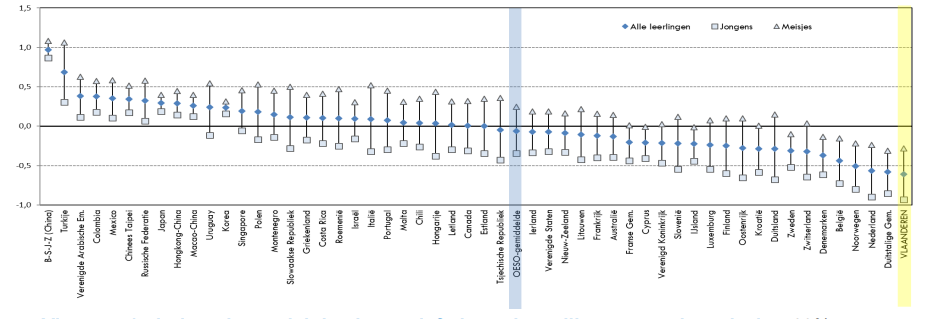
\includegraphics[width=\linewidth]{img/oeso-graphic-leesplezier.png}
	\end{center}
	\caption{Het leesplezier bij 15-jarigen volgens de PISA-test \autocite{DeMeyer2019}.}
	\label{img:oeso-leesplezier}
\end{figure}

Begrijpend lezen valt niet te omzeilen in onze huidige samenleving, maar het leesbegrip verschilt sterk onder studenten in het middelbaar onderwijs. Zo benadrukt \textcite{Vlaanderen2020} dat begrijpend lezen een essentiële vaardigheid is, ook voor vakken buiten Nederlands. Bij wiskunde is begrijpend lezen van cruciaal belang bij complexe vraagstukken. Ook helpt begrijpend lezen studenten om STEM-vakjargon beter te begrijpen.

\medspace 

In het bijzonder hebben scholieren met dyslexie problemen met begrijpend lezen. Onderzoeken van \textcite{Bonte2020, VanDerMeer2022} schatten dat ongeveer 15\% van de Vlaamse scholieren in het middelbaar onderwijs een vorm van dyslexie heeft. Scholieren met dyslexie ervaren moeite en hinder bij het lezen en spellen. Ondanks de bestaande ondersteuning blijven ze toch nog steeds de negatieve impact van hun leerstoornis ervaren. De gevolgen hiervan  kunnen zich doorzetten na het middelbaar onderwijs \autocite{Lissens2020}. Leesvaardigheid blijft daarmee cruciaal voor succes op school en in het werkveld. Scholieren met dyslexie hebben moeilijkheden met deze vaardigheid, wat kan leiden tot onzekerheid en stress. Daarnaast zijn vooroordelen nog steeds een probleem en kunnen ze leiden tot stigmatisering. Echter toont onderzoek aan dat scholieren met dyslexie een sterke doorzettingsvermogen hebben en goede probleemoplossers zijn \autocite{Ghesquiere2018, Lissens2020, Bonte2020}. 

\medspace

Het leerplan voor STEM-vakken stimuleert het gebruik van wetenschappelijke artikelen, maar houdt niet altijd rekening met de bijhorende en complexe leesgraad. De ingewikkelde woordenschat en syntax in wetenschappelijke artikelen kunnen een hindernis vormen voor de begrijpelijkheid van een tekst, aldus \textcite{PlavenSigray2017}. Wetenschappelijke artikelen handmatig vereenvoudigen kan planning, tijd en energie van leerkrachten in het middelbaar onderwijs opslorpen. Het Vlaamse onderwijssysteem staat onder druk en docenten hebben moeite om boven water te blijven. 

\medspace

AI-technologieën zijn vandaag voldoende hoogstaand om tekstvereenvoudiging te automatiseren en om een baanbrekende oplossing te bieden aan het middelbaar onderwijs \autocite{Belpaeme2018}. Het onderwijst past echter zelden soortgelijke technologieën toe. Er is terughoudendheid door enerzijds ouders van leerlingen volgens \textcite{Martens2021a}, anderzijds door de weinige ontwikkelingen in schoolgerelateerde AI-software. Dit terwijl AI-ondersteuning in het onderwijs wel degelijk een positief effect heeft \autocite{Kraft2020}. Er is nood aan een intuïtieve en gebruikersvriendelijke toepassing die taalmodellen of API's kan integreren en aanpassen naargelang de specifieke behoeften van een student met dyslexie. Zo kan dit enerzijds de werkdruk bij leerkrachten verminderen, en anderzijds scholieren in de derde graad ondersteunen bij het lezen van complexe wetenschappelijke artikelen.

\section{\IfLanguageName{dutch}{Onderzoeksvraag}{Research question}}%
\label{sec:onderzoeksvraag}

Dit onderzoek beschrijft het gebruik van AI in de vorm van tekstvereenvoudiging, als advies voor implementatie in het onderwijs. Specifiek om scholieren met dyslexie in de derde graad van het middelbaar onderwijs te ondersteunen bij het begrijpend lezen van wetenschappelijke artikelen. Hiervoor stelt het onderzoek de volgende onderzoeksvraag op: 

\begin{itemize}
	\item Hoe kan een wetenschappelijk artikel automatisch vereenvoudigd worden, gericht op de unieke noden van scholieren met dyslexie in de derde graad middelbaar onderwijs?
\end{itemize}

De oplossingen voor de volgende deelvragen vormen een globaal antwoord op de onderzoeksvraag:

\begin{enumerate}
	% 1
	\item Welke specifieke noden hebben scholieren met dyslexie van de derde graad middelbaar onderwijs bij het begrijpen van complexere teksten? Aanvullend hierop: 
	\begin{itemize}
		\item Wat zijn de specifieke kenmerken van wetenschappelijke artikelen?
	\end{itemize} 
	% 2
	\item Welke aanpakken zijn er voor tekstvereenvoudiging?
	\begin{itemize}
		\item Hoe verloopt de handmatige vereenvoudiging van teksten voor scholieren met dyslexie?
		\item Welke toepassingen, tools en modellen zijn er beschikbaar om Nederlandse geautomatiseerde tekstvereenvoudiging met AI mogelijk te maken?
		\item Hoe is de combinatie van geautomatiseerde tekstvereenvoudiging met gepersonaliseerde  tekstvereenvoudiging mogelijk?
	\end{itemize}
	%4 
	\item Welke functies ontbreken AI-toepassingen om geautomatiseerde tekstvereenvoudiging mogelijk te maken voor scholieren met dyslexie in de derde graad middelbaar onderwijs? 
	\begin{itemize}
		\item Welke manuele methoden voor tekstvereenvoudiging ontbreken in deze tools?
	\end{itemize}
	%3 
	\item Met welke valkuilen bij taalverwerking met AI moeten ontwikkelaars rekening houden?
	% 5
	\item Welk taalmodel of LLM is geschikt voor de ATS van wetenschappelijke artikelen voor scholieren met dyslexie in de derde graad van het middelbaar onderwijs, met dezelfde of gelijkaardige kwaliteiten als gepersonaliseerde MTS?
	% 6
	\item Wat zijn de nodige stappen bij de ontwikkeling van een intuïtieve lokale webtoepassing die zowel scholieren met dyslexie als leerkrachten helpt?
\end{enumerate}


\section{\IfLanguageName{dutch}{Onderzoeksdoelstelling}{Research objective}}%
\label{sec:onderzoeksdoelstelling}

Het onderzoek achterhaalt de technologische en logopedische aspecten waarmee ontwikkelaars rekening meoten houden bij AI-tekstvereenvoudiging. Het resultaat dient als een houvast om hen te begeleiden tijdens de ontwikkeling van deze applicaties voor gepersonaliseerde en geautomatiseerde tekstvereenvoudiging. Verder ontwikkelt het onderzoek een soortgelijke toepassing in het bijzonder voor scholieren met dyslexie in de derde graad van het middelbaar onderwijs. Dit resulteert in een uitgewerkt prototype voor tekstvereenvoudiging, genaamd \textit{Pentimentor}. \textit{Pentimentor} heeft voornamelijk twee functies. Allereerst kan \textit{Pentimentor} wetenschappelijke artikelen vereenvoudigen op basis van de specifieke behoeften van scholieren met dyslexie in de derde graad van het middelbaar onderwijs. Daarnaast biedt \textit{Pentimentor} een geautomatiseerde benadering om wetenschappelijke artikelen op een gepersonaliseerde manier te vereenvoudigen door het gebruik van aanpasbare parameters. Tot slot geeft \textit{Pentimentor} de eindgebruiker het vereenvoudigd artikel terug in Word-formaat. 

\section{\IfLanguageName{dutch}{Opzet van deze bachelorproef}{Structure of this bachelor thesis}}%
\label{sec:opzet-bachelorproef}

De rest van deze scriptie is als volgt opgebouwd:

\begin{itemize}
	\item Hoofdstuk~\ref{ch:stand-van-zaken} geeft een overzicht van de stand van zaken binnen het onderzoeksdomein, op basis van een literatuurstudie.
	\item Hoofdstuk~\ref{ch:methodologie} licht de methodologie toe. Het onderzoek vermeldt de gebruikte onderzoekstechnieken om een antwoord te kunnen formuleren op de onderzoeksdeelvragen. 
	\item Hoofdstuk~\ref{ch:resultaten} bevat de resultaten voor alle onderzoekstechnieken.
	\item Hoofdstuk~\ref{ch:conclusie} geeft de uiteindelijke conclusie en beantwoordt daarmee de onderzoeksvraag.
	\item Tot slot geeft Hoofdstuk~\ref{ch:discussie} verdere aanbevelingen en aanzet voor toekomstig onderzoek binnen de bestudeerde domeinen. 
\end{itemize}

\chapter{\IfLanguageName{dutch}{Stand van zaken}{State of the art}}%
\label{ch:stand-van-zaken}

\section{Inleiding}

Het onderzoek start met een uitgebreide literatuurstudie over de benodigde kennis binnen het logopedisch, taal- en informaticavakdomein om geautomatiseerde en gepersonaliseerde vereenvoudigde teksten te verkrijgen van wetenschappelijke artikelen. Om een toepassing voor gepersonaliseerde en geautomatiseerde tekstvereenvoudiging van wetenschappelijke artikelen  op maat van deze doelgroep aan te reiken, is het van cruciaal belang om de noden van scholieren met dyslexie in de derde graad van het middelbaar onderwijs te benoemen. Het onderzoek benoemt bewezen noden met behulp van een literatuurstudie. Daarnaast kaart het de huidige problemen bij wetenschappelijke artikelen aan. Wetenschappelijke artikelen vereenvoudigen op maat voor scholieren met dyslexie kan volgens taalexperten op verschillende manieren. Het is belangrijk om stil te staan bij de bestaande en reeds bewezen technieken voor \textit{manual text simplification}. Vervolgens komen technieken voor \textit{automated text simplification} aan bod. Zowel de nodige informatie van taalverwerking met AI, als de huidige AI-technologieën voor tekstvereenvoudiging zijn gegeven. Ten slotte zijn AI-technologieën hoogstaand en ontwikkelaars maken deze alsmaar robuuster, maar het is cruciaal om bij dit onderzoek aandacht te besteden aan de mogelijke problemen die AI-ontwikkelaars moeten vermijden of waarvan zij zichzelf attent op moeten maken. 

\section{Specifieke noden en richtpunten}

Om wetenschappelijke artikelen specifiek voor scholieren met dyslexie te vereenvoudigen, moet het onderzoek stilstaan bij de unieke noden van scholieren met dyslexie in de derde graad van het middelbaar onderwijs. Daarnaast moet het onderzoek stilstaan bij de moeilijkheden tijdens het begrijpend lezen van wetenschappelijke artikelen. Deze sectie bespreekt eerst welke technieken en methoden er bestaan om scholieren met dyslexie te ondersteunen tijdens het begrijpend lezen van teksten. Daarna worden de belemmeringen en moeilijkheden van wetenschappelijke artikelen aangekaart. Deze sectie beantwoordt de volgende twee onderzoeksvragen: 

\begin{itemize}
	\item Welke specifieke noden hebben scholieren met dyslexie van de derde graad middelbaar onderwijs bij het begrijpen van complexere teksten?
	\item Wat zijn de specifieke kenmerken van wetenschappelijke artikelen?
\end{itemize}

\subsection{Specifieke noden van scholieren met dyslexie in de derde graad van het middelbaar onderwijs.}

Leesvaardigheid is geen aangeboren vaardigheid, maar iets dat mensen zelf moeten aanleren \autocite{Bonte2020, VanDerMeer2022}. Hoewel dit proces vlot kan verlopen, kunnen mensen met dyslexie benadeeld worden tijdens dit proces.  Dyslexie wordt gekenmerkt door beperkt lezen en kan het voorlezen traag, radend en letter-voor-letter maken. Mensen met dyslexie kunnen tijdens het begrijpend lezen verschillende drempels ervaren. Tabel \ref{table:dyslexia-hurdles} somt deze noden op.

\begin{center}
	\begin{table}[H]
	\begin{tabular}{ | m{9cm} | m{6cm} | } 
		\hline
		\textbf{Kenmerk} & \textbf{Bron} \\ 
		\hline
		Trage woordbenoeming &  \autocite{Bonte2020} \\
		\hline
		Problemen bij het leesbegrip & \autocite{Gala2016, Bonte2020} \\ 
		\hline
		Hardnekkig letter-voor-letter lezen & \autocite{Bonte2020, Zhang2021} \\ 
		\hline
		Problemen met woordherkenning -en herinnering & \autocite{Bonte2020} \\
		\hline
		Moeite bij homofonische of pseudo-homofonische woordenschat & \autocite{Zhang2021} \\
		\hline
		Moeite bij onregelmatige lettergreepcombinaties & \textcite{Gala2016} \\
		\hline
	\end{tabular}
	\caption{Unieke drempels bij scholieren met dyslexie tijdens het begrijpend lezen.}
	\label{table:dyslexia-hurdles}
	\end{table}
\end{center}

De digitalisering evolueerde de voorbije twintig jaar in stijgende lijn en scholieren in de tweede en derde graad zijn, door het gebruik van smartphones en laptops, hier het meeste vatbaar op \autocite{Fernando2021}. Verder omschrijft dit artikel een checklist van technische elementen waaraan een webpagina of toepassing moet voldoen om een leesbare ervaring te voorzien voor scholieren met dyslexie. Tabel \ref{table:dyslexia-necessaries} toont deze noden.

\begin{center}
		\begin{table}[H]
	\begin{tabular}{ | m{9cm} | m{6cm} | } 
		\hline
		\textbf{Kenmerk} & \textbf{Bron} \\
		\hline
		Zachtgele, -groene -of bruine achtergrondkleur 	& \textcite{Santana2012, Rello2017} 	\\ \hline
		Grotere lettergrootte dan 14pt gebruiken		& \autocite{Rello2015} 					\\ \hline
		Woord- en karakterspatiëring verbreden 			& \textcite{Santana2012, Rello2013b} 	\\ \hline
		Consistente lay-out toepassen					& \autocite{Rello2015, Fernando2021} 	\\  \hline
		Waarschuwingen geven omtrent formulieren, sessies (login) & \autocite{Fernando2021}  	\\ \hline
		Duidelijk zichtbare koppen- of headingstructuur & \autocite{Rello2012a} 				\\ \hline
		Duidelijke symbolen of \textit{icons} gebruiken & \autocite{Rello2012} 					\\ \hline
		Inhoud visueel groeperen 						& \autocite{Rello2015, Fernando2021}	\\ \hline
		Huidige positie benadrukken 					& \autocite{Fernando2021} 				\\ \hline
		
	\end{tabular}
	\caption{Noden en oplossingen om webpagina's beter af te stemmen op de mogelijke noden van scholieren met dyslexie.}
	\label{table:dyslexia-necessaries}
	\end{table}
\end{center}

\subsection{Specifieke kenmerken van wetenschappelijke artikelen}

Wetenschappelijke artikelen zijn van cruciaal belang voor het verspreiden van nieuwe kennis en onderzoeksresultaten. Toch blijven ze voor velen een mysterieus en ontoegankelijk gebied, omwille van de complexiteit van de inhoud en het technische jargon dat onmisbaar lijkt te zijn \autocite{Ball2017}. Dit kan het begrip van de artikelen bemoeilijken, vooral bij begrijpend lezen. Daarmee vormt er zich een extra obstakel bij het implementeren van wetenschappelijke artikelen als bron van kennis tijdens de les. Zo volgen wetenschappelijke artikelen IMRAD, een uniform formaat voor gepubliceerde wetenschappelijke artikelen, dat bestaat uit vijf hoofdstukken: samenvatting, inleiding, methodologie, resultaten en discussie. Hoewel het middelbaar en hoger onderwijs deze artikelen gebruiken als leermiddel, is  de inhoud van een hoger niveau en voornamelijk gericht op mensen uit het vakgebied. \textcite{Pain2016, CAS2021} benadrukken de complexiteit van wetenschappelijke artikelen en de volgende aspecten waarom ze moeilijk te interpreteren zijn. Tabel \ref{table:scientific-paper-struggles} somt deze factoren op. Hoewel wetenschappelijke artikelen over een grote drempel bezitten, betrekken ze jongeren met wetenschappelijk onderzoek en leren ze een kritische vaardigheid. 

\begin{center}
	\begin{table}[H]
	\begin{tabular}{| m{4cm} | m{8cm} | m{3cm} | }
		\hline
		\textbf{Probleem} & \textbf{Oplossing} & Bron \\
		\hline
		Veel informatie in een compact formaat of \textit{high information density} & Extra uitleg schrijven bij woorden of compacte zinnen schrijven. & \autocite{Matarese2013, PlavenSigray2017} \\
		\hline
		Hoog gebruik van meerlettergrepige woorden & Synoniemen met minder lettergrepen gebruiken. & \autocite{Siddharthan2006} \\
		\hline
		Wetenschappelijk jargon & Rekening houden met een doelgroep buiten het vakgebied door eenvoudigere synoniemen te schrijven. Indien deze niet beschikbaar zijn, kan er extra uitleg als alternatief worden gegeven. & \autocite{PlavenSigray2017} \\
		\hline
		Complexe concepten & Paragrafen herschrijven zodat ze eerst uitleg geven op een high-level niveau. Vervolgens lagen van complexiteit toevoegen om de lezer te begeleiden doorheen de methodologie, discussie en conclusie van het wetenschappelijk artikel. & \autocite{Pain2016} \\ 
		\hline
		Cijfermateriaal bij resultaten & De interpretatie van percentages of cijfermateriaal schrijven. Zoals 'ongeveer een kwart van de bevolking' in plaats van '24.97\% van de bevolking'. & \autocite{PlavenSigray2017} \\
		\hline
	\end{tabular}
	\caption{Complexe leesfactoren van een wetenschappelijk artikel.}
	\label{table:scientific-paper-struggles}
	\end{table}
\end{center}

Scholieren kunnen over verschillende achtergrondkennis beschikken, wat invloed kan hebben op het tekstbegrip tijdens het begrijpend lezen \autocite{DeMeyer2019}. Zo kunnen scholieren met een achtergrond in fysica sneller de draad oppikken bij het lezen van fysica-gerelateerde artikelen dan scholieren met een economische achtergrond. Dit maakt het moeilijk om de leesbaarheid van een tekst objectief te beoordelen. Het jargon kan voor de ene groep scholieren makkelijk zijn, en voor de andere groep moeilijk.

\medspace

Onderzoeken en ontwikkelaars zorgen voor de ontwikkeling van geautomatiseerde berekening van leesmetrieken en leesgraadsscores. Zo kunnen ontwikkelaars dit doen met python-libraries via commandline of CLI-toepassingen, waaronder Textstat\footnote{https://pypi.org/project/textstat/} en Readability\footnote{https://pypi.org/project/readability/}. Tabel \ref{table:readability-scores} toont drie prevalente leesgraadscores weer. Daarnaast kunnen toepassingen, zoals Textinspector\footnote{https://textinspector.com/} of Charactercalculator\footnote{https://charactercalculator.com/}, analytisch inzicht geven in de complexiteit van Engelstalige teksten. Deze toepassingen kunnen echter geen Nederlandstalige teksten of leesmetrieken analyseren. Hoewel deze leesmetrieken een beknopte analyse kunnen vormen voor taaldeskundigen, toch benadrukken onderzoekers dat deze leesgraadscores geen rekening houden met de achtergrondkennis van mogelijke lezers, aldus \autocite{Cantos2019}. Recent onderzoek van \textcite{Crossley2019} achterhaalt de mogelijkheid om geautomatiseerde taalverwerking te gebruiken voor leesmetrieken die wel rekening houden met de doelgroep. Hoewel deze modellen potentieel tonen, kunnen ontwikkelaars deze nog niet gebruiken \autocite{Crossley2019}.

\begin{center}
	\begin{table}[H]
	\begin{tabular}{ | m{5cm} | m{10cm} | } 
		\hline
		\textbf{Score} & \textbf{Uitleg} \\ 
		\hline
		Flesch Reading Ease (FRE) & Deze leesgraadscore berekent de moeilijkheidsgraad op zinbasis. Hoe hoger de score, hoe 'eenvoudiger' de zin \autocite{Cantos2019, Readable2021}. \\
		\hline
		Gunning FOG (FOG) & In tegenstelling tot FRE, berekent FOG de moeilijkheidsgraad op basis van de volledige tekst \autocite{Cantos2019}. \\
		\hline
		Complexe woordenlijst volgens \textit{Dale-Chall Index} (DCI) & Deze lijst omvat woorden die experimenten bij Amerikaanse tieners als complex omschrijven. De DCI werkt per leeftijdscategorie \autocite{Cantos2019}. \\
		\hline
	\end{tabular}
	\caption{Leesgraadscores volgens onderzoek van \textcite{Cantos2019}.}
	\label{table:readability-scores}
	\end{table}
\end{center}

Divers onderzoek van de afgelopen tien jaar wijzen uit dat wetenschappelijke teksten steeds complexer worden. Dat maakt deze teksten voor niet-experten en niet-doctoraatsstudenten minder toegankelijk, vanwege het gebruik van technisch jargon en ingewikkelde zinsstructuren \autocite{Ball2017, PlavenSigray2017, Jones2019}. Deze trend begon volgens onderzoek al in de tweede helft van de twintigste eeuw \autocite{Hayes1992}.

\medspace

Volgens onderzoek van \textcite{PlavenSigray2017} maken wetenschappers en onderzoekers onbewust wetenschappelijke artikelen moeilijker om te lezen. Uit een vergelijkende studie tussen abstracten en de rest van de inhoud van wetenschappelijke tijdschriften blijkt dat abstracts het meest complexe deel van een artikel vormen. De evolutie van de leesbaarheid wordt weergegeven in figuur \ref{img:fre-ndc}. Deze figuur toont de FRE (links) en NDC (rechts) scores. Zo schat het onderzoek dat 22\% van alle wetenschappelijke artikelen op het niveau van een masterstudent in het Engels geschreven zijn, tegenover 14\% in 1960. Deze trend is belangrijk om op te volgen in de komende decennia, omdat het een obstakel kan vormen voor toekomstige generaties.

\begin{figure}[H]
	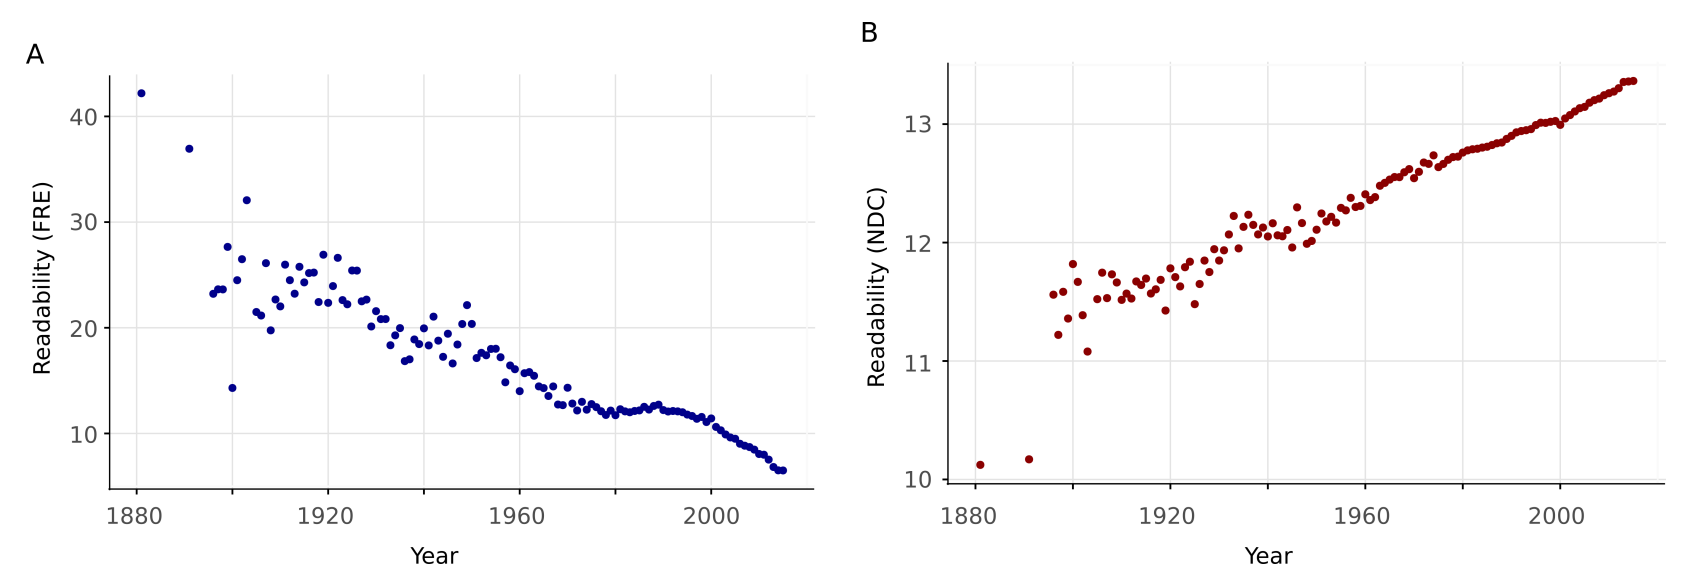
\includegraphics[width=\linewidth]{img/fre-ndc.png}
	\caption{De toename van benodigde leesgraad voor het lezen van wetenschappelijke artikelen. Bron: \autocite{PlavenSigray2017}}
	\label{img:fre-ndc}
\end{figure}

Onbegrijpelijke en ontoegankelijke zinsstructuren hinderen ook vakexperten. Zo toonde onderzoek van \textcite{McNutt2014} aan dat begrip van de methodologie en resultaten cruciaal is in het kader van reproduceerbaarheid; enkel zo kunnen wetenschappers op correcte wijze een studie reproduceren en wetenschappelijke inzichten bevestigen of met verdere resultaten verrijken. Experimenten van \textcite{Hubbard2017} wijzen namelijk uit dat het net vooral de methodologie en resultaten van een wetenschappelijk artikel zijn die een hoge leesgraad vergen. In deze context zijn de onderzoeken van \textcite{Hartley1999} en \textcite{Snow2010} relevant waarin ze aantonen dat het herschrijven van abstracts de begrijpbaarheid ervan kan verhogen.

\medspace

Volgens \textcite{Hollenkamp2020} moeten vereenvoudigde of samengevatte wetenschappelijke artikelen drie vragen kunnen beantwoorden: waarom werd het onderzoek uitgevoerd, wat zijn de experimenten en wat zijn de conclusies van de onderzoekers? Dit omvat de achtergrondinformatie, hypotheses, methoden, resultaten, implicaties, beperkingen en aanbevelingen. De tekst omzetten in een ander formaat zoals post-it notes, tabelvorm of opsommingen, maakt het beter begrijpbaar \autocite{Rijkhoff2022}. 

\medspace

Wetenschappelijke artikelen zijn voornamelijk in pdf-formaat terug te vinden. Dit formaat valt eenvoudig in te lezen met python-pakketten, zoals PDFMiner of PyPDF. Wel ondervinden ontwikkelaars soms problemen bij het inlezen van pdf-bestanden, aldus \textcite{Lee2021}. Tools kunnen niet alle tekstinhoud uit een pdf extraheren. Als oplossing kunnen ontwikkelaars gebruik maken van \textit{optical character recognition} of OCR. Ondertussen bestaan er python-bibliotheken die deze technologie met een eenvoudige implementatie kunnen uitwerken, namelijk EasyOCR\footnote{https://pypi.org/project/easyocr/} en Tesserat \autocite{Lee2021}.

\medspace

Bovendien bestaat de uitvoer van deze artikelen uit louter losse tekstblokken. Het systeem is niet in staat om automatisch te identificeren welke delen titels, afbeeldingen of tekstblokken zijn. Een mogelijke oplossing hiervoor is het gebruik van \textit{LayoutParser}\footnote{https://pypi.org/project/layoutparser/}. Dit is een \textit{deep learning} of DL-model dat zorgvuldige \textit{Document Image Analysis} uitvoert. Met behulp van \textit{LayoutParser}, in samenwerking met het Detectron2\footnote{https://ai.meta.com/blog/-detectron2-a-pytorch-based-modular-object-detection-library-/}-algoritme, is het mogelijk om de tekstinhoud van wetenschappelijke artikelen te extraheren. Figuur \ref{img:layoutparser} geeft een voorbeeld weer waarbij het model de tekstblokken van drie verschillende soorten documenten, waaronder een wetenschappelijk artikel links in beeld, markeert en classificeert. Met reeds vermelde OCR-technieken kan het systeem deze omkaderde tekst inlezen en gebruiken in dergelijke toepassingen \autocite{Shen2021}.

\begin{figure}[H]
	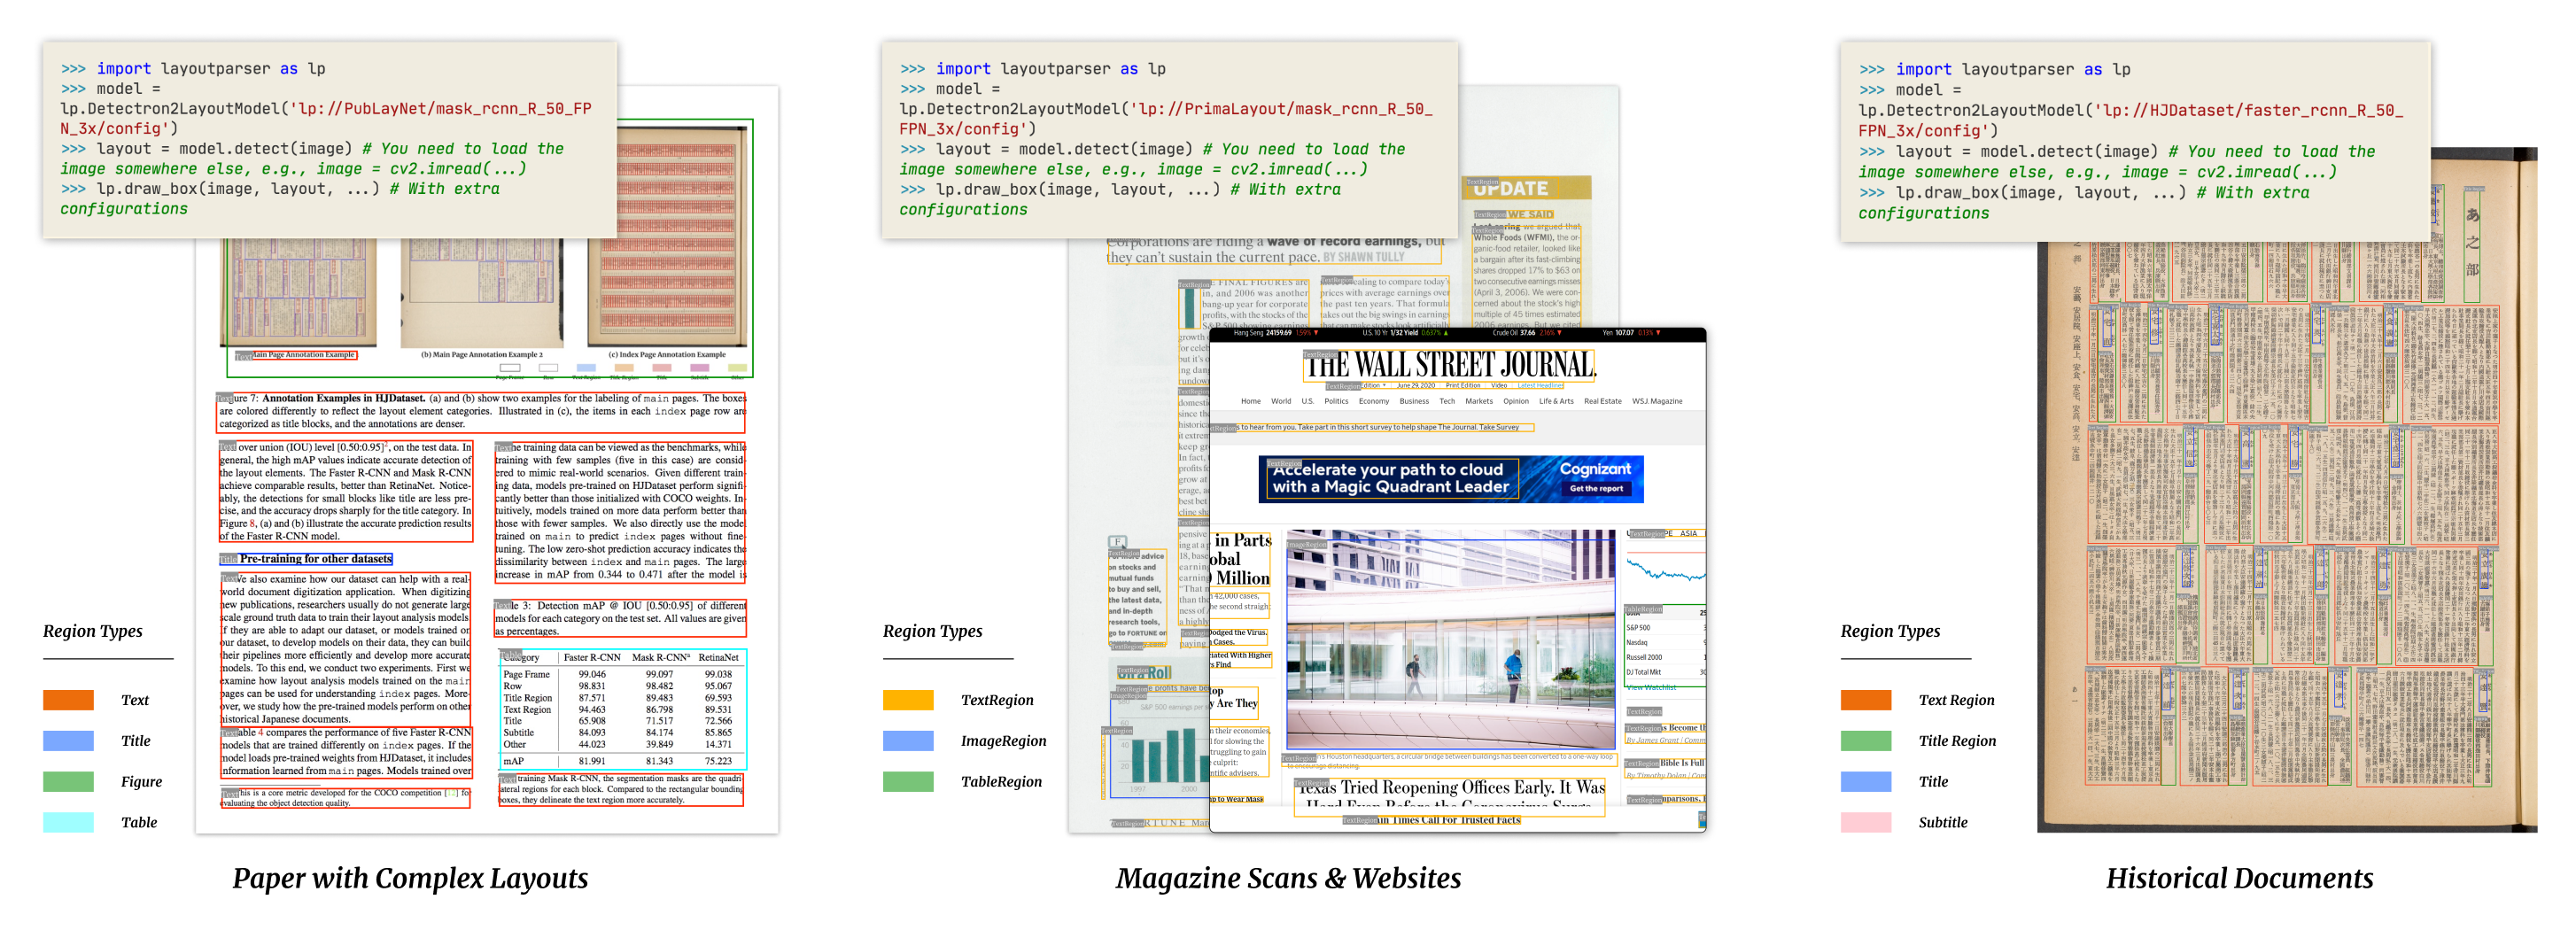
\includegraphics[width=\linewidth]{img/layoutparser.png}
	\caption{LayoutParser toepassen op drie verschillende documenten. De kaders geven verschillende geclassificeerde tekstblokken aan. Bron: \autocite{Shen2021}.}
	\label{img:layoutparser}
\end{figure} 

\subsubsection{Conclusie}

In deze eerste sectie van de literatuurstudie zocht het onderzoek naar de specifieke behoeften van scholieren met dyslexie in de derde graad van het middelbaar onderwijs. Verder stond het stil bij de moeilijkheden die zij ervaren bij het begrijpend lezen van wetenschappelijke artikelen. Zo wijst de literatuurstudie de volgende technieken en methoden om hen te ondersteunen bij het begrijpend lezen. Tabellen \ref{table:dyslexia-necessaries} en \ref{table:dyslexia-hurdles} geven een overzicht van deze technieken en methoden. Daarnaast omschrijven onderzoeken ook specifieke kenmerken van wetenschappelijke artikelen die het begrip ervan bemoeilijken, opgesomd in tabel \ref{table:scientific-paper-struggles}. Tot slot kunnen ontwikkelaars en vakexperten de complexiteit van een tekst berekenen met bestaande leesgraadscores, zoals beschreven in tabel \ref{table:readability-scores}.

\section{Aanpakken voor tekstvereenvoudiging}

\subsection{Manuele tekstvereenvoudiging}
% Hoe worden teksten handmatig vereenvoudigd voor scholieren met dyslexie? 

Voor sommige lezers kan het begrijpend lezen van een complexe tekst echter een uitdaging zijn, zoals scholieren met dyslexie. \textit{Manual tekst simplification} of MTS kan deze groep helpen \autocite{Siddharthan2014}. De techniek van MTS gebruikt eenvoudige woordenschat en zinsstructuren en maakt structurele aanpassingen (SA) om de tekst vlotter leesbaar te maken. MTS is het proces dat het technische leesniveau en het woordgebruik van een geschreven tekst vermindert. Dit resulteert tot een betere leeservaring zonder het verlies van de kerninhoud tijdens het lezen van de tekst. Tabel \ref{table:manual-simplification} toont een overzicht van bewezen MTS-technieken, zonder een specifiek toespitsing op een doelgroep.

\begin{center}
		\begin{table}[H]
			\begin{tabular}{ | m{2.5cm} | m{8cm} | m{4.5cm} | } 
			\hline
			\textbf{Type vereenvoudiging} & \textbf{Techniek} & \textbf{Bron} \\ \hline
			
			LS & Moeilijke woorden vervangen door eenvoudigere synoniemen & \autocite{Crossley2012, Rello2013c, Siddharthan2014} \\ 
				& Woorden- en synoniemenlijst maken & \autocite{Siddharthan2006, Bosmans2022b} \\
				& Dubbelzinnige woorden vervangen & \\
				& Idiomen vervangen & \autocite{Siddharthan2006} \\ 
				& Regelmatige lettergreepcombinaties gebruiken & \autocite{Gala2016} \\
				& Rekening houden met het gekende jargon van de doelgroep & \autocite{JavoureyDrevet2022} \\
			\hline
			SS & Tangconstructies aanpassen & \autocite{Bosmans2022c} \\
			& Zinnen langer dan tien woorden inkorten & \autocite{Siddharthan2014} \\
			& Verwijswoorden aanpassen & \autocite{Bosmans2022a} \\
			& Voorzetseluitdrukkingen aanpassen & \autocite{Rello2013d} \\
			& Samengestelde werkwoorden aanpassen & \autocite{Bosmans2022b} \\
			& Actieve stem gebruiken & \autocite{Ruelas2020} \\
			& Onregelmatige werkwoorden vermijden & \autocite{Rello2013d, Gala2016} \\
			\hline
			SA & Marges aanpassen & \autocite{Rello2013d} \\
			& Lettertype -en grootte aanpassen & \autocite{Rello2012a} \\
			& Woord- en karakterspatiëring aanpassen & \autocite{Rello2012a} \\
			& Herschrijven als opsomming of tabelvorm & \autocite{Rello2015} \\
			\hline
		\end{tabular}
		\caption{Drie algemene technieken voor MTS bij een algemene doelgroep.}
		\label{table:manual-simplification}
	\end{table}
\end{center}

\subsection{Bevoordelende effecten van MTS bij scholieren met dyslexie}

Onderzoek toont aan dat vereenvoudigde teksten het leesbegrip en woordherkenning van kinderen met dyslexie significant kunnen verbeteren \autocite{RiveroContreras2021}. Bovendien blijkt uit experimenten dat frequent woordgebruik de decodeertijd bij mensen met dyslexie significant vermindert, en dat teksten met verminderde lexicale complexiteit minder leesfouten opleveren voor mensen met dyslexie \autocite{Rello2013a, Gala2016}. De studie van \textcite{Gala2016} benadrukt ook moeilijkheden van kinderen met dyslexie bij het lezen van woorden met onregelmatige lettergreepcombinaties. Mensen zonder dyslexie bereiken doelwaarden onder optimale omstandigheden, zoals aangegeven door de richting van de pijl op figuur \ref{img:readability-mean-fixation-duration}. Het gebruik van veelvoorkomende woorden vermindert de decodeertijd en verbetert het leesbegrip voor mensen met dyslexie.

\begin{figure}
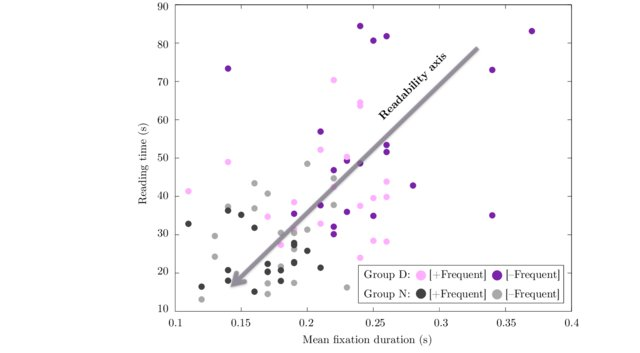
\includegraphics[width=\linewidth]{img/readability-mean-fixation-duration.png}
\caption{De gemeten \textit{mean fixation duration} tijdens het begrijpend lezen van teksten uit het onderzoek van \textcite{Rello2013a}.}
\label{img:readability-mean-fixation-duration}
\end{figure}

Hoewel onderzoeken de positieve effecten van lexicale vereenvouding voor lezers met dyslexie onderstrepen, is er relatief weinig onderzoek gedaan naar de effecten van syntactische vereenvoudiging op kinderen en scholieren met dyslexie. In het experiment van \textcite{Linderholm2000} had het aanpassen van causale structuren een significant effect op het leesbegrip en de foutenmarge van de bevraagden met een lage leesgraad. Het onderzoek van \textcite{Leroy2013} onderzoek het effect van herstelde coherentieonderbrekingen en plaatste tekst in een logische volgorde. Zo konden zowel vaardige als minder vaardige lezers profiteren van de revisies. Verbaal parafraseren had geen significant effect op lezers met dyslexie, volgens \textcite{Rello2013c}. De bevraagden waren tijdens het onderzoek tussen de 13 en 37 jaar oud, met een gemiddelde leeftijd van 21 jaar. Het tekstformaat bleef ongewijzigd, maar lettertypes werden aangepast.

\medspace

Het onderzoek van \textcite{Nandhini2013} experimenteerde met een andere vorm van aanpassingen om de leesbaarheid van teksten te verhogen, namelijk gepersonaliseerde samenvattingen. Het experiment in het onderzoek maakt gebruik van onaangepaste zinnen uit de oorspronkelijke tekst die op maat van de lezer zijn gepresenteerd en herstructureert deze volgens de oorspronkelijke tekst. Door de belangrijkste zinnen onaangepast te laten en de structuur aan te passen, is de tekst toegankelijker voor de lezer. Hoewel de onderzoekers de rusulterende logische structuur in twijfel trokken, was de leesbaarheid van teksten bij de deelnemers significant beter dan bij de oorspronkelijke tekst, zonder negatieve effecten op het leesbegrip.

\medspace

Tot slot hebben onderzoeken aangetoond dat scholieren met dyslexie gevoeliger zijn voor veranderingen in visuele parameters, zoals lettertype, karakterafstand, tekst- en achtergrondkleur en grijswaarden. Minimalistische ontwerpen met pictogrammen behoren tot de aanbeveling om de leesbaarheid te verbeteren, evanals lettergrootte groter dan 14pt en een \textit{sans-serif}, \textit{monospaced} of \textit{roman} lettertype \autocite{Rello2013b}. Volgens \textcite{Rello2015, Bezem2016, Rello2017} zijn lichtgrijze achtergronden met zwart lettertype op een gele achtergrond, of zachtgele, -groene of lichtblauwe achtergrondkleuren de beste kleurencombinaties. Het gebruik van lettertypen zoals OpenDys heeft geen effect op lezers met of zonder dyslexie, terwijl cursieve lettertypen worden afgeraden, aldus \textcite{Rello2013b, Rello2015}.

\medspace

Tabel \ref{table:benefits-mts} somt de bewezen strategieën op samen met de bewezen voordelen tijdens het begrijpend lezen.

\begin{center}
	\begin{table}[H]
	\begin{tabular}{ | m{5cm} | m{5cm} | m{5cm} | } 
	\hline
	\textbf{Techniek} & \textbf{Bewezen voordeel} & \textbf{Bron}\\
	\hline
	Frequent woordgebruik & Lagere decodeertijd & \autocite{Rello2013a, Gala2016} \\
	& Beter leesbegrip & \autocite{Rello2013a, Gala2016} \\
	\hline	
	Verwerpen van onregelmatige lettergrepen & Verminderde decodeertijd & \autocite{Gala2016} \\
	& Beter leesbegrip & \autocite{Gala2016} \\	
	\hline
	Causale structuren aanpassen & Beter leesbegrip & \autocite{Linderholm2000} \\
	& Minder fouten bij het begrijpend lezen & \autocite{Linderholm2000} \\
	\hline	
	Tekstgebeurtenissen in een tijdsafhankelijke volgorde plaatsen & Beter leesbegrip bij het reviseren & \autocite{Leroy2013} \\
	\hline
	Coherentieonderbrekingen herstellen & Beter leesbegrip bij het reviseren & \autocite{Leroy2013} \\
	\hline
	Gepersonaliseerde samenvatting & Betere leesbaarheid & \autocite{Nandhini2013} \\
	\hline
	Zachtkleurige achtergrond & Betere leesbaarheid & \autocite{Rello2015} \\
	\hline
	Niet-cursieve, sans-serif lettertypen & Betere leesbaarheid & \autocite{Rello2013b} \\
	\hline 
	Lettertype groter dan 14pt & Betere leesbaarheid & \autocite{Rello2013b} \\
	\hline
	\end{tabular}
	\caption{Bewezen voordelen van MTS op mensen met dyslexie tijdens het begrijpend lezen.}
	\label{table:benefits-mts}
	\end{table}
\end{center}

\subsection{Aanpak voor ATS.}
% Welke toepassingen, tools en modellen zijn er beschikbaar om Nederlandse geautomatiseerde tekstvereenvoudiging met AI mogelijk te maken? 

De laatste evolutie in machinaal leren biedt een mogelijkheid om dit proces te automatiseren. \textit{Automatic text simplification} of ATS is een onderdeel van natuurlijke taalverwerking binnen machinaal leren (ML). Dit omvat technieken zoals tekstanalyse, taalherkenning -en generatie, spraakherkenning -en synthese en semantische analyse. NLP stelt computers in staat om menselijke taal te begrijpen en te communiceren op een natuurlijke manier. De begrippen die volgen worden behandeld in \textcite{Sohom2019, Eisenstein2019} en zijn cruciaal voor de daaropvolgende concepten.

\medspace

Zo dient tokenisatie om zinnen op basis van tokens te splitsen. Er zijn vier manieren om tokens in een tekst te splitsen en zo een woordenschat op te bouwen, namelijk op woord-, karakter-, subwoord- en zinniveau, volgens onderzoek van \textcite{Menzli2023}. Bij karaktertokenisatie neemt de inputlengte toe, maar dit heeft volgens \textcite{Ribeiro2018} weinig bruikbare \textit{use cases}. Het opsplitsen van zeldzame woorden in kleinere stukken om een woordenschat op te bouwen biedt voordelen ten opzichte van woordtokenisatie, aldus \autocite{Iredale2022}.

\medspace

In NLP baseert het lemmatiseren zich op stemming, een NLP-taak waarbij deze de stam van een woord neemt, maar ook rekening houdt met de betekenis van elk woord. Er zijn Nederlandstalige modellen beschikbaar voor lemmatiseren, zoals JohnSnow\footnote{https://nlp.johnsnowlabs.com/2020/05/03/lemma\_nl.html}. Omgekeerd lemmatiseren werkt door een afgeleide vorm van de stam te bepalen, bijvoorbeeld enkelvoud of meervoud voor zelfstandige naamwoorden als ’hond’ \autocite{Eisenstein2019}. Bij het parsen krijgt elk woord of zinsdeel een label toegewezen, zoals zelfstandig naamwoord, bijwoord, werkwoord, bijzin of stopwoord. De identificatie van zinsdelen heet chunking. Parsing is vatbaar op ambiguïteit omdat bijvoorbeeld ‘een plant’ niet gelijk is aan de vervoeging van het werkwoord ’planten’ \autocite{Eisenstein2019}.

\medspace

Om de betekenis van elk woord in een tekst te begrijpen, moet een machine in staat zijn om de betekenis achter elk token te begrijpen. Dit is waar \textit{sequence labeling} om de hoek komt kijken, volgens \textcite{Eisenstein2019}. Elk woord in een tekst krijgt een label voor \textit{Part-of-Speech} (PoS) of \textit{Named-Entity-Recognition} (NER). Deze fase van NLP achterhaalt de structuur van een tekst. PoS-tagging richt zich op de grammaticale categorieën van woorden, terwijl NER-labeling zich richt op het herkennen van specifieke entiteiten in een tekst. Bij PoS-tagging worden de woorden in een zin geanalyseerd. Elk woord krijgt een koppeling aan een grammaticale categorie, zoals een zelfstandig naamwoord, werkwoord, bijvoeglijk naamwoord of bijwoord. \textit{PoS-tagging} helpt bij het begrijpen van de syntactische structuur van een zin en is nuttig bij parsing en machinevertaling. Een voorbeeld van PoS-tagging is te zien in figuur \ref{fig:pos-labeling} en is afkomstig uit \textcite{Bilisci2021}.

\begin{center}
	\begin{figure}[H]
		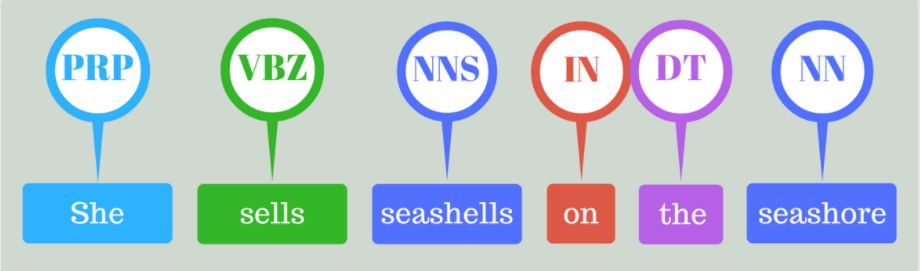
\includegraphics[width=15cm]{img/poslabeling.png}
		\caption{Voorbeeld van PoS-labeling uit het artikel van \textcite{Bilisci2021}.}
		\label{fig:pos-labeling}
	\end{figure}
\end{center}

Met NER-labeling kunnen systemen zo namen van personen, organisaties en locaties herkennen en classificeren. Het haalt specifieke informatie uit een tekst, zoals het identificeren van de namen van personen, plaatsen of bedrijven die in nieuwsartikelen, of het extraheren van belangrijke data of getallen uit financiële rapporten, aldus \textcite{Jurafsky2014}. Er zijn vier vormen van NER-labeling, zoals beschreven door \textcite{Li2018}: \textit{dictionary-based}, \textit{rule-based}, \textit{ML-based} en \textit{deep learning-based}. De eerste twee maken gebruik van vooraf gedefinieerde woordenboeken en regels, terwijl de laatste twee gebruik maken van statistische of neurale netwerken om te leren hoe entiteiten te herkennen. Elke vorm maakt gebruik van representaties om entiteiten te modelleren. \textcite{Poel2008} hebben een neuraal netwerkmodel onderzocht voor PoS-tagging van Nederlandstalige teksten. Het model behaalde een nauwkeurigheid van 97,88\% voor bekende woorden en 41,67\% voor onbekende woorden en maakte gebruik van de Corpus Gesproken Nederlands (CGN) als trainingsdata. In de verwerking van tekst maken NLP-systemen gebruik van embeddings om woorden numeriek te representeren. Traditionele word embeddings bouwen een woordenschat op zonder de betekenis ervan in context te begrijpen. Contextuele word embeddings begrijpen wel de context van een woord \autocite{Eisenstein2019}. 

\section{De verschillende soorten ATS}

Tekstvereenvoudiging kan bijdragen aan het begrijpen van complexe informatie. Zoals onderzocht door \textcite{Siddharthan2014}, zijn er vier soorten transformaties bij ge- automatiseerde tekstvereenvoudiging, waaronder lexicale vereenvoudiging, waarbij eenvoudigere synoniemen de complexe woorden vervangen. Dit heet \textit{lexical simplification} (LS) of lexicale vereenvoudiging. Bijvoorbeeld, ‘klevend’ kan ‘adhesief’ vervangen. \textcite{Kandula2010} noemt twee manieren om lexicale vereenvoudiging te bewerkstelligen: het vervangen van het woord door een synoniem of het genereren van extra uitleg. De zinsstructuur blijft hetzelfde en de kerninhoud en benadrukking van de tekst blijven behouden. Het doel van lexicale vereenvoudiging is om de moeilijkheidsgraad van de woordenschat in een zin of tekst te verlagen.

\medspace

Diverse onderzoeken hebben aangetoond dat lexicale vereenvoudiging een belangrijke bijdrage kan leveren aan het begrijpen van complexe informatie, en in dit kader wordt de pipeline zoals weergegeven in figuur \ref{img:pipeline-lexical-simplification} vaak gebruikt, bijvoorbeeld in onderzoeken van \textcite{Paetzold2016, Bingel2018, Bulte2018}. Deze pipeline omvat bij de vermelde onderzoeken telkens minstens vier stappen, waarbij de eerste stap \textit{Complex Word Identification} (CWI) is, een gesuperviseerde NLP-taak die moeilijke woorden of \textit{multi-word expressions} (MWE) in een tekst identificeert \autocite{Shardlow2013, Gooding2019}. De LS, waarbij eenvoudigere synoniemen de moeilijkere woorden vervangen, komt na CWI. Hier kunnen ook verklarende beelden of definities komen \autocite{Zeng2005, Kandula2010}. Een goede uitvoering is van cruciaal belang bij CWI, omdat een lage recall van dit component zal resulteren in een uitvoertekst zonder vereenvoudiging van moeilijke woorden zoals opgemerkt door \textcite{Shardlow2013}. Er zijn verschillende manieren geïdentificeerd om substitutiegeneratie uit te voeren, zoals opgesomd in tabel \ref{table:lexical-databases}. Recenter onderzoek, zoals dat van \textcite{Zhou2019}, gebruikt ook een extra \textit{Substitution Ranking} (SR) stap om substituties te rangschikken op basis van relevantie. 

\begin{figure}[H]
	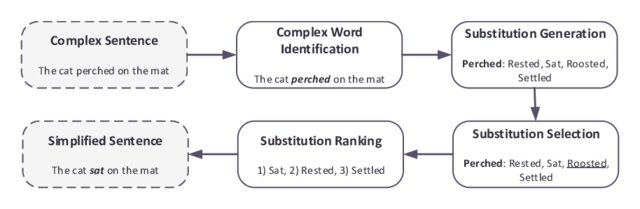
\includegraphics[width=15cm]{img/lexical-simplification-pipeline.png}
	\caption{Een pipeline voor LS volgens \textcite{Althunayyan2021}.}
	\label{img:pipeline-lexical-simplification}
\end{figure}

\begin{center}
\begin{table}[H]
	\begin{tabular}{ | m{7cm} | m{7cm} | } 
		\hline
		\textbf{Databank} & \textbf{Ondersteunde talen} \\
		\hline
		Engels & WordNet \\
		& SWORDS \\
		& LSBert \\
		\hline
		Nederlands & Celex \\
		& NT2Lex \\
		& Cornetto \\
		\hline
		Meertalig (Engels, Duits, Spaans en Portugees) & PHOR-in-One \\
		\hline	
	\end{tabular}
	\caption{Beschikbare Nederlandstalige, Engelstalige en meertalige lexicale databanken anno mei 2023.}
	\label{table:lexical-databases}
\end{table}
\end{center}

\textit{Syntactic simplification} (SS) of syntactische vereenvoudiging is een techniek om de complexiteit van een zin te verminderen. Het past de grammatica en zinsstructuur van de tekst aan. Dit gebeurt door het combineren van twee zinnen tot één eenvoudigere zin of door de syntax te vereenvoudigen, terwijl de semantiek bewaren blijft. \textcite{Kandula2010} onderzochten de ontwikkeling van dergelijk model voor medische informatie. Het model bestaat uit drie modules, die zinnen met meer dan tien woorden vereenvoudigen en eventueel vervangen door kortere zinnen. Het omvat een \textit{PoS Tagger}, een Grammar Simplifier en een Output Validator als onderdelen van de architectuur.

\begin{enumerate}
	\item Ten eerste wordt de \textit{PoS Tagger}-functie uit het open-source pakket OpenNLP\footnote{https://opennlp.apache.org/} gebruikt.
	\item Vervolgens splitst de \textit{Grammar Simplifier}-module lange zinnen in kortere zinnen door middel van het identificeren van POS-patronen en het toepassen van transformatieregels.
	\item Tot slot controleert de \textit{Output Validator}-module de grammatica en leesbaarheid van de output van de Grammar Simplifier.
\end{enumerate}  

ATS is geen nieuw concept. Volgens onderzoeken van \textcite{Canning2000, Siddharthan2006} zijn de eerste aanpakken op ATS gebouwd op rule-based modellen. Deze modellen bewerken de syntax door zinnen te splitsen, te verwijderen of de volgorde van de zinnen in een tekst aan te passen. LS komt hier niet aan de pas. Recentere onderzoeken van \textcite{Coster2011, Bulte2018} verduidelijken hoe ontwikkelaars LS en SS kunnen combineren.

\medspace

Vroegere onderzoeken tonen aan dat geautomatiseerde tekstvereenvoudiging al geruime tijd bestaat. Zo hebben \textcite{Canning2000} en \textcite{Siddharthan2006} onderzocht dat de eerste methoden gebaseerd waren op \textit{rule-based} modellen die de syntaxis van de tekst bewerken door zinnen te splitsen, te verwijderen of te herschikken. Lexicale vereenvoudiging speelde hierbij geen rol. Enkel de recentere onderzoeken van  Pas bij recentere onderzoeken, zoals die van \textcite{Coster2011, Bulte2018} tonen de mogelijkheid aan om LS en SS te combineren.

\medspace

Om wetenschappelijke artikelen toegankelijker en begrijpelijker te maken, is het van belang om de kernpunten van een artikel op een duidelijke en beknopte manier samen te vatten. Hoewel samenvatten niet gericht is op het vereenvoudigen van de tekst, is het wel een techniek die noodzakelijk is om de semantiek achter een tekst met zo min mogelijk woord- of tekens te kunnen begrijpen. Full-text-search en gepersonaliseerde informatiefiltering benadrukken het belang van deze op maat gemaakte samenvattingen. Een samenvattingssysteem bestaat uit drie fases: analyse van de brontekst, identificatie van de kernpunten en samenvoeging van deze kernpunten tot één overzichtelijke tekst. Het machinaal samenvatten van teksten kan op twee manieren: door extractie en door abstractie \autocite{Hahn2000, Dubay2004}.

\medspace

Het proces van extraherend samenvatten markeert de belangrijkste zinnen in een tekst en herschrijft ze. Dit kan echter leiden tot onsamenhangende uitvoertekst, zoals \textcite{Khan2014} heeft aangetoond. Er zijn verschillende methoden beschikbaar om de kernzinnen te bepalen, zoals woordfrequentie, zinpositie -en gelijkenissen, de \textit{cue}-methode, titels, \textit{proper nouns}, woordgebruik en de afstand tussen \textit{text unit entities}, aldus \textcite{Khan2014}. Verschillende technieken voor het extraherend samenvatten van teksten, waaronder graafgebaseerde methoden, maximal marginal relevance (MMR) en metaheuristiek gebaseerde ES, zijn onderzocht door \textcite{Verma2020}. Tabel \ref{table:extractive-summarization} omschrijft deze drie methoden verder.

\begin{center}
	\begin{table}[H]
	\begin{tabular}{ | m{4cm} | m{12cm} | } 
		\hline
		MMR-gebaseerde ES & Deze techniek gebruikt de maximaal marginale relevantiescore (MMR) om de relevantie en diversiteit van gemarkeerde zinnen te bepalen. Dit voorkomt dat geselecteerde zinnen elkaar niet overlappen in inhoud en relevantie. Deze methode kan leiden tot betere samenvattingen, maar vereist meer rekenkracht en tijd dan de andere twee technieken. \\
		\hline
		Graafgebaseerde ES & Deze techniek vertegenwoordigt een document als een graaf van zinnen. Deze vorm gebruikt algoritmen om de belangrijkste zinnen te bepalen en redundantie te vermijden. Dit kan zowel voor lange wetenschappelijke artikelen als korte nieuwsartikelen goede resultaten opleveren \autocite{McDonald2007, Lin2010}. \\ 
		\hline
		Metaheuristiek-gebaseerde ES & Deze techniek maakt gebruik van optimalisatie-algoritmen om de belangrijkste zinnen in een tekst te vinden \autocite{Premjith2015, Verma2020}. Evaluatiefuncties kunnen echter afhankelijk van de gebruikte criteria in een lokaal optimum vastlopen \autocite{Rani2021}. \\
		\hline
	\end{tabular}
	\caption{Drie manieren om extraherende samenvatting mogelijk te maken volgens \textcite{Verma2020}.}
	\label{table:extractive-summarization}
	\end{table}
\end{center}

Vooroordelen of \textit{bias} kan de extraherende samenvatting van nieuwsartikelen beïnvloeden, zo blijkt uit experimenten uitgevoerd door \textcite{McKeown1999}. Deze vorm van samenvatten neemt de zinnen over zoals ze zijn. \textcite{Hahn2000} bouwden verder op deze experimenten door het combineren van \textit{knowledge-rich} en \textit{knowledge-poor} methoden, wat resulteerde in significante verbeteringen. Bij het extraherend samenvatten is het van belang om de meest relevante tekstgedeeltes te selecteren, meestal in de vorm van zinnen. Om de lexicale en statistische relevantie van een zin te kunnen bepalen, noemen \textcite{Hahn2000} twee methoden:

\begin{itemize}
	\item Het lineaire gewichtsmodel, waarbij elke teksteenheid wordt gewogen op basis van factoren zoals de positie van de zin en het aantal keren dat deze voorkomt.
	\item Het gewichtsmodel op basis van de statistische relevantie van een eenheid, waarbij rekening wordt gehouden met de aanwezigheid van woorden in titels.
\end{itemize}

Om de nauwkeurigheid van modellen te verbeteren, ontwikkelden \textcite{Nallapati2017} \textit{SummaRuNNer}. Dit model kan teksten extraherend samenvatten door een neuraal netwerk. Zo gebruikt het \textit{PyTorch} en bestaat het uit drie modellen: een recurrent neuraal netwerk, een convolutioneel recurrent neuraal netwerk en een \textit{hiërarchical attention network}.

\medspace

Extraherende samenvattingen kunnen leiden tot een onsamenhangende tekst. Abstraherende samenvatting kan een oplossing bieden, omdat het rekening houdt met de samenhang van een tekst. Onderzoek van \textcite{Gupta2019} wijst twee benaderingen voor abstraherende samenvatting: semantisch-gebaseerd en structuurgebaseerd. De structuurgebaseerde methode gebruikt regels om belangrijke informatie in de tekst te vinden, maar dit kan leiden tot samengevatte zinnen van lage taalkundige kwaliteit en grammaticale fouten. De semantisch-gebaseerde benadering daarentegen gebruikt de betekenis van de tekst om korte en duidelijke samenvattingen te maken met minder redundante zinnen en een betere taalkundige kwaliteit. Een extra parsingfase kan van pas komen volgens de onderzoeken. Onderzoeken van \textcite{Suleiman2020, Cao2022} wijzen \textit{deep learning}-methoden uit om automatisch abstraherende samenvattingen te genereren. Zo kunnen RNN's, CNN's en Seq2Seq dienen om abstraherende samenvatting mogelijk te maken. 

\medspace

Ontwikkelaars moeten een andere aanpak gebruiken wanneer zij een systeem willen ontwikkelen voor \textit{long text summarization} of LTS, zoals bij boeken of wetenschappelijke tijdschriften. Zo kan het opsplitsen van de tekst leiden tot het breken van samenhangende paragrafen. Dat kan later resulteren in redundante tekst in het samengevatte document. Zo raadden onderzoeken van \textcite{Hsu2018, Huang2019} aan om zowel extraherend als abstraherende samenvatting toe te passen. Om deze reden zou een \textit{hybrid summarization pipeline} twee fasen moeten bevatten: een inhoudselectiefase waarbij het systeem kernzinnen extraheert, gevolgd door een parafraserende fase.

\medspace

Tot slot moeten ontwikkelaars rekening houden met de doelgroep wanneer zij een systeem of model uitkiezen voor tekstvereenvoudiging of samenvatting. Zo moeten ontwikkelaars rekening houden met de individuele behoeften en uitdagingen van elke scholier, volgens \textcite{Gooding2022}. Dyslexie kan zich namelijk op verschillende manieren uiten bij verschillende scholieren, waarbij bijkomende symptomen niet altijd van invloed zijn op de spellingprestaties van een scholier. Om deze reden is het belangrijk om een toepassing te ontwerpen die rekening houdt met de diversiteit van dyslexie.

\section{Beschikbare tools en taalmodellen}
\label{sec:beschikbare-tools-en-taalmodellen}

Het kan moeilijk zijn voor scholieren met dyslexie om goed te lezen en te schrijven. Gelukkig zijn er verschillende softwareprogramma's en tools beschikbaar om hen te ondersteunen. Deze sectie gaat in op de nationale en internationale software die specifiek is ontworpen voor scholieren met dyslexie om hen te helpen bij het lezen van teksten.  Er zal voornamelijk worden gekeken naar beschikbare software in Vlaamse middelbare scholen, chatbots zoals Bing Chat en ChatGPT, en software die speciaal is ontwikkeld om dyslexie bij het lezen te ondersteunen. Deze sectie beantwoordt de volgende deelvraag: 

\begin{itemize}
	\item Welke toepassingen, tools en modellen zijn er beschikbaar om Nederlandstalige geautomatiseerde tekstvereenvoudiging met AI mogelijk te maken?
\end{itemize}

Scholieren met dyslexie krijgen in het middelbaar onderwijs enkel ondersteuning in de vorm van voorleessoftware \autocite{DeCraemer2018, OnderwijsVlaanderen2023}. Het ministerie van Onderwijs in Vlaanderen biedt licenties aan voor verschillende softwarepakketten zoals SprintPlus, Kurzweil3000, Alinea Suite, IntoWords en TextAid, die scholieren kunnen gebruiken om zinnen te markeren en deze vervolgens samen te vatten. Het samenvatten gebeurt echter op een manier waarbij de zinnen lexicaal en syntactisch identiek blijven. Helaas bieden deze softwarepakketten geen functie voor het vereenvoudigen van teksten. Volgens \textcite{Tops2018} is het belangrijk om deze software zo vroeg mogelijk in de schoolcarrière te introduceren, zodat scholieren er snel vertrouwd mee raken en het optimaal kunnen gebruiken in verdere studies. Hoewel \textcite{Tops2018} de handige aspecten van deze software benadrukt, is het te laat om deze software pas in het hoger onderwijs te introduceren.

\medspace

Momenteel beschikken de voorleessoftware beperkte LS-functionaliteiten. Dit onderstreept de noodzaak aan nieuwe erkende tools die tekstvereenvoudiging in het onderwijs mogelijk maken. Tools zoals Simplish en Rewordify kunnen een oplossing bieden. Hoewel Simplish oorspronkelijk Engelstalig is, kan het inmiddels vereenvoudigde teksten genereren van Nederlandstalige teksten. Deze functionaliteit is echter enkel betalend voor niet-Engelstalige teksten. Vervolgens kan Rewordify enkel Engelstalige teksten vereenvoudigen. Tot slot vindt de literatuurstudie weinig online \textit{proof-of-concepts} terug. Daarnaast bieden de toepassingen geen transparantie over hun gebruikte taalmodel, waardoor ontwikkelaars de logica en werking van deze toepassingen niet kunnen reproduceren. 

\medspace

Voor samenvatting zijn er echter meer tools beschikbaar. Enkele voorbeelden hiervan zijn Resoomer, Paraphraser, Editpad, Scribbr en Quillbot. Al zijn er onderzoeken over ATS-technieken voor scholieren met dyslexie, het aantal onderzoeken over samenvatten voor deze doelgroep is schaars. Zoals eerder aangehaald is er wel onderzoek gedaan naar de verschillende manieren om een tekst samen te vatten, maar er is geen toepassing of onderzoek dat dit concreet uitwerkt. \textcite{Sanja2021} wijzen erop dat toepassingen voor tekstvereenvoudiging regelmatig als \textit{showcase} van de technologie ontwikkeld worden en zelden tot weinig rekening houden met gepersonaliseerde samenvatting om zo rekening te houden met de verschillende noden.

\medspace

Er zijn weinig toepassingen beschikbaar om wetenschappelijke artikelen te vereenvoudigen, maar er bestaan gratis en betalende toepassingen. Zo reiken SciSpace\footnote{https://typeset.io/} en Scholarcy\footnote{https://www.scholarcy.com/} ATS specifiek voor wetenschappelijke artikelen aan. Hero vloeide verder uit het onderzoek van \textcite{Bingel2018}, waarbij de onderzoekers een toepassing voor gepersonaliseerde ATS voor kinderen met dyslexie ontwikkelden. Hoewel Hero een oplossing aanreikt, slaagt de toepassing er niet in om wetenschappelijke artikelen te vereenvoudigen. Wel kunnen scholieren deze browserextensie gebruiken voor selecte Engelstalige nieuwssites. Tabel \ref{table:overview-tools} geeft een overzicht van prevalente tools die momenteel tekstvereenvoudiging aanbieden.

\begin{center}
	\begin{table}[H]
		\begin{tabular}{ | m{4cm} | m{11cm} | } 
		\hline
		\textbf{Tool} & \textbf{Algemene functionaliteit} \\
		\hline
		Sprintplus & \\
		Kurzweil3000 & \\
		Alinea Suite & Voorleessoftware met ondersteuningsmogelijkheden voor moeilijke woordenschat \\
		IntoWords & \\
		TextAid & \\
		\hline
		Resoomer &  \\
		Paraphraser & \\
		Editpad & Samenvattingstool \\
		Scribbr & \\
		Quillbot & \\
		\hline
		SciSpace & Samenvattingstool specifiek voor wetenschappelijke artikelen. \\
		Scholarcy & \\
		\hline
		Simplish & Tool voor tekstvereenvoudiging met bijhorende analyse\\
		Rewordify & \\
		\hline
		\end{tabular}
	\caption{Overzicht van gekende voorleessoftware, tekstvereenvoudigings- en samenvattingstools die intuïtief zijn ontwikkeld voor de eindgebruiker (leerkracht of scholier).}
	\label{table:overview-tools}
	\end{table}
\end{center}

Ontwikkelaars kunnen ook zelf aan de slag gaan. Zo beschikt HuggingFace (HF) een breed scala aan API's en tools die gemakkelijk te downloaden en trainen zijn voor \textit{pretrained} modellen voor veelvoorkomende NLP-taken, zoals \textit{text classification}, taalmodellering en samenvatting. Tekstvereenvoudiging is in mindere mate aanwezig. Verder kunnen ontwikkelaars deze modellen \textit{finetunen} op specifieke datasets om modellen te bouwen voor gepersonaliseerde NLP-taken. Tot slot geeft tabel \ref{table:huggingface-models} HF-taalmodellen met hun respectievelijke casus. De volgende taalmodellen neemt de tabel op: Google Pegasus\footnote{https://ai.googleblog.com/2020/06/pegasus-state-of-art-model-for.html}, Longformer Encoder-Decoder\footnote{https://huggingface.co/docs/transformers/model\_doc/led}, Simplification\footnote{https://huggingface.co/haining/scientific\_abstract\_simplification}, BART Large Scientific Summarisation\footnote{https://huggingface.co/sambydlo/bart-large-scientific-lay-summarisation}, T5 finetuned text simplification model\footnote{https://huggingface.co/husseinMoh/t5-small-finetuned-text-simplification} en Keep It Simple\footnote{https://huggingface.co/philippelaban/keep\_it\_simple}

\begin{center}
	\begin{table}[H]
	\begin{tabular}{ | m{4cm} | m{12cm} | } 
		\hline
		\textbf{Taalmodel} & \textbf{Specifieke casus} \\ \hline
		Google Pegasus & Samenvattingstaken voor kort tot middelgrote documenten. \\
		\hline
		Longformer Encoder-Decoder (LED) & Samenvatting van lange wetenschappelijke artikelen \\
		\hline
		Haining Scientific Abstract Simplification & Het lexicaal vereenvoudigen van wetenschappelijke artikelen. \\
		\hline
		BART Large Scientific Summarisation & Het samenvatten van wetenschappelijke artikelen. \\
		\hline
		T5 finetuned text simplification model & Tekstvereenvoudiging voor algemeen gebruik. \\
		\hline
		Keep It Simple & Ongesuperviseerde tekstvereenvoudiging met ATS. \\
		\hline
	\end{tabular}
		\caption{Beschikbare en ge-finetunede HF-taalmodellen.}
		\label{table:huggingface-models}
	\end{table}
\end{center}

Dankzij de sterke evolutie in data en AI, kon de grootte van deze taalmodellen sterk vergroten. Zo is GPT-3 een opkomend \textit{Large Language Model} of LLM. OpenAI ontwikkelde dit taalmodel en paste daarvoor een tweestapsleerparadigma toe \autocite{Radford2019, Li2022}. 

\begin{itemize}
	\item Allereerst komt er een ongesuperviseerde training aan bod met een \textit{language modelleing goal}. Ontwikkelaars trainden dit model op niet-gecategoriseerde data van het internet met datasets zoals Common Crawl, WebText2, Books1, Books2 en Wikipedia.
	\item Tenslotte finetunen de ontwikkelaars dit verder. Om een correcte respons van het model te krijgen, passen de ontwikkelaars \textit{reinforcement learning} toe.
\end{itemize}

GPT-3 beschikt over meerdere versies, waaronder GPT-3.5 die als engine dient voor ChatGPT. Omdat onbegrijpelijke en ontoegankelijke zinsstructuren niet alleen voor leken, maar ook voor vakexperten een obstakel vormen, is het belangrijk om te benadrukken dat GPT-3.5 gericht is op conversationele doeleinden, terwijl GPT-3 in het algemeen bedoeld is om met hoogstens één prompt te werken \autocite{McNutt2014, Hubbard2017}. Verder reikt OpenAI documentatie uit voor het GPT-3 taalmodel. Daarin vermelden ze vier \textit{engines}, namelijk Davinci, Curie, Babbage en Ada. In maart 2023 kwam daar een vijfde engine bij, namelijk GPT-3 Turbo die fungeert als achterliggende engine voor Chat-GPT. Davinci-003 is het meest geavanceerde model, geschikt voor taken zoals het schrijven van essays en het genereren van code, en levert de meest menselijke antwoorden. Curie is goed in nuance, maar minder menselijk dan Davinci, terwijl Ada en Babbage minder krachtig zijn en beter geschikt zijn voor eenvoudige taken zoals het aanvullen van tekst en sentimentanalyse \autocite{Brockman2023}. Deze engines gebruiken dezelfde set hyperparameters, die ontwikkelaars kunnen aanpassen. Tabel \ref{table:gpt-3-parameters} somt deze parameters verder op.

\begin{center}
	\begin{table}[H]
	\begin{tabular}{ | m{2.5cm} | m{7cm} | m{4.5cm} | }
		\hline
		\textbf{Parameter} & \textbf{Omschrijving} & \textbf{Mogelijke waarden} \\ \hline
		\textit{model} & De GPT-3 engine die ontwikkelaars kunnen gebruiken. & davinci, curie, babbage, ada, text-davinci-002, text-curie-001, text-babbage-001, text-ada-001, davinci-codex \\ \hline
		\textit{temperature} & De gulzigheid van het generatief model. Een lagere waarde kan voorspelbare tekst teruggeven. Hogere waarden daarentegen kunnen onverwachtse tekst teruggeven, wat beter werkt bij creatieve toepassingen. & Een kommagetal tussen 0 en 1. \\ \hline
		\textit{max tokens} & Het maximaal aantal tokens (woorden of subwoorden) dat het generatief model kan teruggeven. & Een getal tussen 1 and 2048. \\ \hline
		\textit{top-p} & Vergelijkbaar met temperature, maar deze waarde onderhoudt de \textit{probability distribution} voor \textit{common tokens}. Hoe lager de waarde, hoe hoger de woordfrequentie van de gegenereerde tekst. Toepassingen gericht op nauwkeurigheid maken beter gebruik van hoge waarden. & Een kommagetal tussen 0 en 1. \\
		\hline
		stop & Een tekstwaarde (woord/symbool) tot waar het model zal genereren. & String-waarden \\
		\hline
		\textit{presence penalty} & Factor die bepaalt hoe regelmatig woorden voorkomen & Kommagetallen tussen 0 en 1 \\
		\hline
	\end{tabular}
		\caption{Tabel met alle GPT-3 parameters.}
		\label{table:gpt-3-parameters}
	\end{table}
\end{center}

Hoewel onderzoeken rond GPT-3 nog volop in ontwikkeling zijn, bestaan er vergelijkende onderzoeken naar de mogelijkheden van dit LLM. Onderzoek van \textcite{Binz2023} wijst uit dat de mean-regret score kan dienen als maatstaf om de menselijkheid van antwoorden te beoordelen. Deze studie wees verder uit dat deze modellen capabel zijn om menselijke antwoorden te produceren, zoals geïllustreerd in figuur \ref{img:mean-regret-chatgpt}. Uit het experiment van \textcite{Goyal2022} blijkt dat \textit{zero-shot} samenvattingen met GPT-3 beter presteren dan gefinetunede modellen. \textcite{Li2022} benadrukt dat GPT-3 overkill is voor sentimentanalyse. Daarvoor haalt het onderzoek aan om een kleinschaliger taalmodel te gebruiken. Daarnaast beschikken LLM's over een grotere ecologische voetafdruk, waarvoor onderzoeken van \textcite{Strubell2019, Simon2021} deze praktijk ook afraden. Uiteindelijk bestaan er al enkele tools die gebruikmaken van de GPT-3 API, waaronder Jasper AI en ChatSonic zoals aangehaald in het onderzoek van \textcite{Mottesi2023}. Experten zoals \textcite{Roose2023, Garg2022} halen het GPT-3 model en ChatGPT aan als de toekomst voor gepersonaliseerde en adaptieve uitleg aan scholieren. Bing Chat biedt een extra dat revolutionair kan zijn bij het opzoeken van uitleg voor zoektermen, zonder het verlies aan bronvermelding. Dankzij de personalisering van de prompts biedt GPT-3 mogelijkheden aan voor toepassingen in het onderwijs, aldus \textcite{Roose2023, Garg2022}.

\begin{figure}[H]
	\begin{center}
		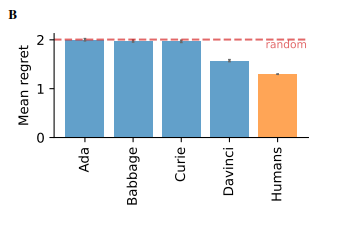
\includegraphics[width=\linewidth]{img/chatgpt-engines-mean-regret.png}
		\caption{Een experiment op de \textit{mean-regret} van GPT-3 engines uit \textcite{Binz2023}.}
		\label{img:mean-regret-chatgpt}
	\end{center}
\end{figure}

Met neurale netwerken kan het taalmodel patronen in de input herkennen. Deze patronen dienen om voorspellingen te maken over de output \autocite{Liu2020}. Via prompts hebben mensen toegang tot krachtige taalmodellen, zoals GPT-3 of BERT \autocite{McFarland2023, Harwell2023}. Figuur \ref{img:prompt-engineering} illustreert de werking van deze vaardigheid. Onderzoek van \textcite{Liu2020} benadrukt het belang van goed opgestelde prompts. Hiervoor kunnen eindgebruikers de technieken in tabel \ref{table:techniques-for-good-prompts}. Zo moeten deze werk kunnen produceren op maat van het doel. Zo benadrukt de onderzoeker dat een prompt concreet moet zijn. Bij het opstellen van een prompt voor een zoekopdracht is het cruciaal om voldoende parameters op te nemen om te voorkomen dat het model te algemeen blijft en afwijkt van de intentie van de gebruiker. Effectieve prompt engineering voor AI leidt tot hoogwaardige trainingsgegevens, waardoor het AI-model nauwkeurige voorspellingen en beslissingen kan maken \autocite{Liu2020}.

\begin{table}
	\begin{tabular}{| m{5cm} | m{5cm} | }
		\hline
		\textbf{Prompttechniek} & \textbf{Bron} \\ \hline
		Duidelijke scope & \autocite{McFarland2023} \\ \hline
		Specifieke sleutelwoorden & \autocite{McFarland2023} \\ \hline
		De context waarin de vraag zich afspeelt. & \autocite{McFarland2023} \\ \hline
		Gepersonaliseerde keuzes & \autocite{McFarland2023} \\ \hline
	\end{tabular}
	\caption{Technieken voor concrete en goed opgestelde prompts.}
	\label{table:techniques-for-good-prompts}
\end{table}

\begin{figure}[H]
	\begin{center}
		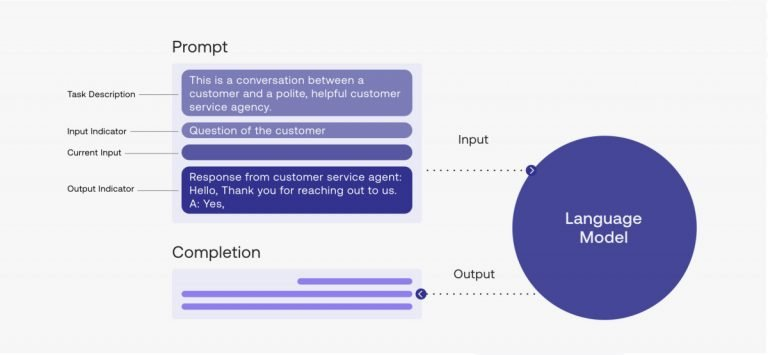
\includegraphics[width=\linewidth]{img/prompt-engineering-medium.png}
	\end{center}
	\caption{De werking van \textit{prompt engineering} volgens \textcite{McFarland2023}}
	\label{img:prompt-engineering}
\end{figure}

Om prompts te kunnen hergebruiken, bouwden ontwikkelaars \textit{prompt patterns} op. Deze patronen bieden herbruikbare oplossingen voor veelvoorkomende problemen in een bepaalde context, vooral bij de interactie met LLM's. \textcite{White2023} benoemt vier \textit{prompt patterns}:

\begin{itemize}
	\item	\textit{Intent prompts} waarbij een LLM een instructie krijgt met een specfiek verwacht antwoord.
	\item	\textit{Restriction prompts} die het antwoord van een LLM inperkt. Deze pattern is noodzakelijk om een LLM binnen de lijnen te houden.
	\item 	\textit{Contextualization prompts} verzekeren dat de output van een LLM relevant is. De prompt bevat de context.
	\item	\textit{Expansion/reduction prompts} genereren een beknopte output met voldoende details. 
\end{itemize}

BERT is een meertalige LLM die gebruikmaakt van \textit{contextual word embeddings}. Onderzoekers trainden het model op 110 miljoen parameters uit 104 verschillende talen, waaronder Nederlands. Voor de Nederlandse taal zijn er twee varianten van BERT beschikbaar: RobBERT en BERTje. GPT-3 en BERT beschikken over een verschillende architectuur. Zo is volgens \textcite{Mottesi2023} GPT-3 een autoregressief model die alleen rekening houdt met de linkercontext bij het voorspellen of genereren van tekst. BERT daarentegen is een bidirectioneel model, waarbij het model zowel de linker- als de rechtercontext in overweging neemt. De bidirectionele werking van BERT is geschikt voor sentimentanalyse, waarbij begrip van de volledige zincontext noodzakelijk is. Omdat GPT-3 toegang heeft tot meer informatie (45 TB) dan BERT (3 TB), kan dit een voordeel bieden tijdens taalbewerkingen zoals vereenvoudigen, parafraseren of vertalen. Tot slot verschillen de LLM's ook qua grootte. Hoewel beide modellen erg groot zijn, is GPT-3 aanzienlijk groter dan BERT, mede door de uitgebreide trainingsdatasetgrootte \autocite{Brown2020}. Er is echter een nieuw generatief taalmodel genaamd LLaMa, dat sterker is dan GPT-3 en vergelijkbare modellen, terwijl het slechts tien keer minder parameters gebruikt. Helaas is LLaMa momenteel nog niet beschikbaar als online webtoepassing of API \autocite{Hern2023, Touvron2023}. Figuur \ref{img:graph-language-models} toont de evolutie van \textit{pre-trained} taalmodellen. Zo volgt de LLM-performantie ten opzichte van het aantal parameters van een LLM een lineaire functie.

\begin{figure}[H]
	\begin{center}
		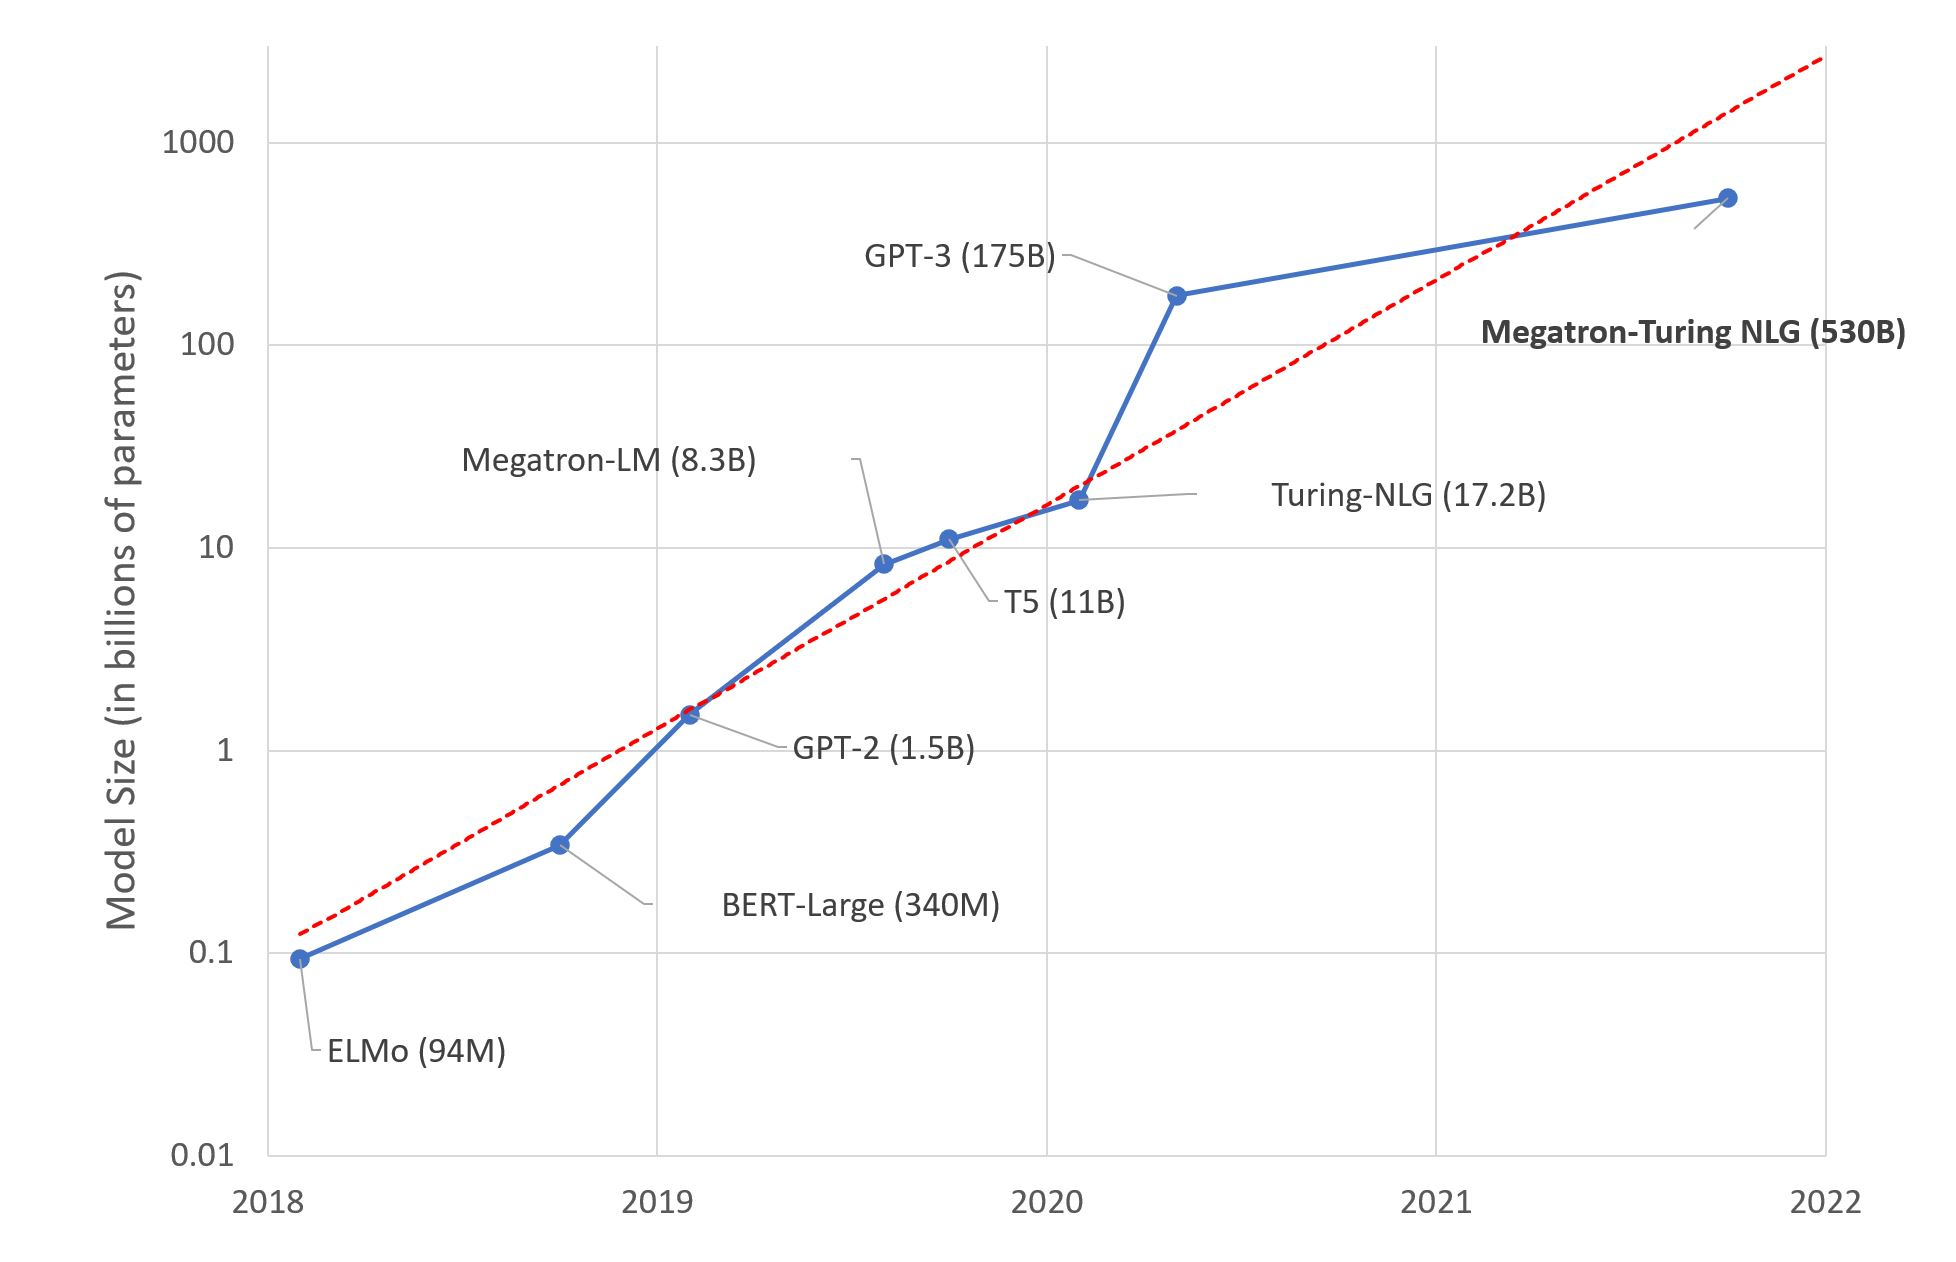
\includegraphics[width=\linewidth]{img/graph-language-models.png}
		\caption{De evolutie van LLM's. Bron: \autocite{Simon2021}}
		\label{img:graph-language-models}
	\end{center}
\end{figure}

Microsoft en OpenAI werken nauw samen. Zo gebruikt Bing Chat ook het GPT-3 taalmodel. Met de Prometheus-technologie kan deze chatbot verder bouwen en verwijzingen bieden naar andere websites \autocite{Ribas2023}. Zo maakt Bing Chat verwijzingen naar bestaande online documenten dankzij de Bing index-, ranking- en antwoordresultaten. Prometheus combineert dit met het redeneervermogen van OpenAI’s GPT-modellen. Via de \textit{Bing Orchestrator} genereert Prometheus iteratief een set \textit{internal queries} om zo binnen de gegeven gesprekscontext nauwkeurige antwoorden op gebruikersvragen te bieden \autocite{Ribas2023}. Bing Chat is beschikbaar als webpagina en browserextensie voor Microsoft Edge. Het gebruik van extraherende en abstraherende samenvattingen maakt de chatbot interessant, al bestaat er nog te weinig onderzoek naar de credibiliteit en correctheid van de verstrekte verwijzingen. Daarnaast beschikt Bing Chat niet over een API, waardoor ontwikkelaars geen CLI-toepassingen met deze technologie kunnen maken.

\section{De valkuilen bij AI en NLP.}

AI en ML zijn volop in groei. NLP gebruikt AI en ML om menselijke taal te verwerken, terwijl NLU deze technologieën gebruikt om menselijke taal te begrijpen. Hoewel deze technologieën veelbelovend zijn, moeten AI-ontwikkelaars rekening houden met veelvoorkomende en genegligeerde uitdagingen en valkuilen \autocite{Sciforce2020, Roldos2020, Khurana2022}. Deze sectie beantwoordt de volgende onderzoeksvraag: 

\begin{itemize}
	\item Met welke valkuilen bij taalverwerking met AI moeten ontwikkelaars rekening houden?
\end{itemize}

Het ontwikkelen van NLP- en NLU-toepassingen is duur en vormt een obstakel voor IT-professionals vanwege factoren zoals het gebrek aan NLP-expertise, de kwaliteit en kwantiteit van data, de integratie en deployment van modellen en de transparantie van modellen \autocite{IBM2022}. Bij de ontwikkeling en finetuning van een NLP-toepassing met AI verkiezen software-ontwikkelaars \textit{black-box} modellen. Hoewel het verschil in nauwkeurigheid minimaal is, wordt de afweging gemaakt op basis van de transparantie van het model. Na een transformatie wordt niet aangegeven waarom specifieke transformaties zijn uitgevoerd, zoals het vervangen van een woord door een eenvoudiger synoniem. \textit{White-box} taalmodellen zijn schaars \autocite{Punardeep2020}.

\medspace 

Homoniemen kunnen \textit{sequence labeling} bemoeilijken, zoals beschreven in onderzoek door \textcite{Roldos2020}. Een voorbeeld hiervan is het woord 'bank', dat voor de machine niet duidelijk aangeeft of het gaat om de financiële instelling of het meubelstuk. Methoden zoals \textit{Word Sense Disambiguation} (WSD), \textit{PoS-tagging} en \textit{contextual embeddings} kunnen de betekenis van woorden bepalen op basis van de context \autocite{Eisenstein2019, Liu2020}. Het verbeteren van NLP-systemen met synoniemen en antoniemen kan worden bereikt door het gebruik van \textit{candidate generation} en synoniemherkenning, terwijl meertalige transformers zoals BERT een oplossing bieden voor de beperkte toepassingen in andere talen dan het Engels \autocite{Dandekar2016, Roldos2020}.

\medspace

Verschillende studies tonen aan dat MTS en ATS gelijke kansen kunnen bieden aan iedereen. Bij de ontwikkeling van gepersonaliseerde ATS-toepassingen moeten ontwikkelaars de ethische overwegingen en de behoeften van de eindgebruiker in overweging nemen, zoals beschreven in onderzoeken van \textcite{Niemeijer2010, Xu2015, Gooding2022}. Om de eindgebruiker meer controle te geven, moet deze eindgebruiker kunnen kiezen welke delen van de tekst het systeem moet vereenvoudigen.

\medspace

Hoewel iedereen kan converseren met een chatbot, vereist het verkrijgen van gepaste en verwachte antwoorden een doordachte input. Onnauwkeurige prompts of een gebrek aan trainingsdata kunnen leiden tot onjuiste output. Door het gebruik van conditionele expressies of het finetunen van hyperparameters kan echter de betrouwbaarheid van de antwoorden worden vergroot \autocite{Miszczak2023, Jiang2023}.

\medspace

Het beoordelen van vereenvoudigde teksten vereist de nodige opvolging van ontwikkelaars in vergelijking met andere ML- of NLP-taken. Evaluatiemetrieken zoals ROUGE en BLEU zijn beperkt omdat ze geen rekening houden met de semantiek tussen een referentietekst en een vereenvoudigde of samengevatte tekst. Om dit probleem op te lossen, beveelt \textcite{Fabbri2020} aan dat ontwikkelaars menselijke evaluatie inschakelen om de vereenvoudigde tekst van een taalmodel te beoordelen. De onderzoekers dringen aan op verdere studie naar nieuwe standaarden en beste praktijken voor betrouwbare menselijke beoordeling. Bovendien moeten de doelgroepen voor wie de tekst wordt vereenvoudigd, nauw betrokken worden bij het proces \autocite{Iskender2021}. Tabel \ref{table:summary-hurdles} somt de aangehaalde struikelblokken bij de ontwikkeling van NLP-toepassingen op.

\begin{center}
	\begin{table}[H]
	\begin{tabular}{ | m{4cm} | m{10cm} | }
		\hline
		\textbf{Probleem} & \textbf{Oplossing} \\
		\hline
		Dure ontwikkeling en onderhoud van taalmodellen & Voorkeur voor black-box modellen bij ontwikkeling en finetuning. API's kunnen als alternatief dienen op zelf-gehoste taalmodellen. \\
		\hline
		Homoniemen kunnen \textit{sequence labeling} bemoeilijken & Word Sense Disambiguation, PoS-tagging en contextual embeddings. \\
		\hline
		Paternalisme & Ontwikkeling van gepersonaliseerde tekstvereenvoudigingstoepassingen moeten de eindgebruiker meer controle geven, zoals het kiezen welke delen van de tekst vereenvoudigd moeten worden, het gebruik van synoniemen of het markeren van zinnen die moeilijk te begrijpen zijn. \\
		\hline
		Onnauwkeurige prompts & Gebruik van conditionele expressies bij prompts of one-shot summary uitvoeren. \\
		\hline
		Onnauwkeurige evaluatie van tekstvereenvoudiging & Menselijke evaluatie toepassen of gebruik maken van ROUGE-L metrieken die wel de semantiek in achting nemen. \\
		\hline
	\end{tabular}
	\caption{Samenvattend schema met vaak voorkomende struikelblokken bij NLP-toepassingen.}
	\label{table:summary-hurdles}
	\end{table}
\end{center}

\section{Conclusie}

Tot slot beantwoordt de literatuurstudie de onderzoeksdeelvragen. Zo is begrijpend lezen voor scholieren met dyslexie in de derde graad van het middelbaar niet enkel moeizaam, maar gaat verder dan dat. Deze scholieren kunnen moeite ondervinden bij het ontcijferen en automatiseren van woordherkenning. MTS en aangepaste opmaakopties bieden bewezen voordelen voor scholieren met dyslexie. Het gebruik van vakjargon, ingewikkelde woordenschat en moeizame syntax sluiten een algemeen publiek uit en maken het enkel mogelijk voor wetenschappelijk geletterden om deze artikelen te lezen. Zo kunnen MTS-technieken, besproken in \ref{table:benefits-mts}, scholieren met dyslexie helpen bij het begrijpend lezen van wetenschappelijke artikelen. Tabel \ref{table:scientific-paper-struggles} somt alle complexe leesfactoren op, alsook hoe lezers deze moeilijke materie kunnen aanpakken. Deze twee tabellen moeten dienen als aftoetscriteria bij de ontwikkeling van een prototype voor gepersonaliseerde ATS. 

\medspace

Er zijn taalmodellen beschikbaar in de vorm van API's of open-source software die deze transformaties kunnen uitvoeren. De overheid leent voornamelijk leessoftware uit, maar LLM's bieden mogelijkheden aan voor gepersonaliseerde ATS. Zo kunnen de achterliggende taalmodellen van ChatGPT en Bing Chat specifieke vragen verwerken. Het onderzoek moet verschillende prompts kunnen vergelijken bij het uittesten van dit taalmodel. Verschillende LS, SS en SA-technieken moeten in deze vergelijkende studie aan bod komen. 

\medspace

Gerichte menselijke vergelijkingen en leesbaarheidsformules dienen als evaluatie voor de vereenvoudigde teksten door ATS. De python-bibliotheek \textit{readability} biedt de leesgraadscores, zoals weergegeven in \ref{table:readability-scores}, aan voor ontwikkelaars. Zo kan dit onderzoek de uitvoer van verschillende teksten vergelijken met een objectieve maatstaf.

\medspace

Tot slot geeft tabel \ref{table:summary-hurdles} een overzicht van struikelblokken waarmee ontwikkelaars rekening moeten houden. In het kader van ATS voor wetenschappelijke artikelen, moet het taalmodel gebruikmaken of voldoende getraind zijn op data van wetenschappelijke artikelen en vereenvoudigde versies van diezelfde wetenschappelijke artikelen. Als het onderzoek gebruik maakt van een promptgebaseerd model, dan moeten deze prompts op maat gemaakt zijn voor scholieren met dyslexie in de derde graad van het middelbaar onderwijs. Tot slot moet dergelijk prototype ook de gebruiker de vrijheid krijgen om teksten te markeren waarvan deze persoon een vereenvoudigde versie wilt.

%%=============================================================================
%% Methodologie
%%=============================================================================

\chapter{\IfLanguageName{dutch}{Methodologie}{Methodology}}%
\label{ch:methodologie}

% Door de vergaarde kennis uit de literatuurstudie in hoofdstuk \ref{ch:stand-van-zaken} over de mogelijke noden van scholieren met dyslexie, de complexiteit van wetenschappelijke artikelen, de technieken voor MTS en ATS, en de bijhorende valkuilen bij taalverwerking met AI, kunnen onderzoeksmethoden worden toegepast om een antwoord te vinden op de onderzoeksvraag. 

De vergaarde kennis uit de literatuurstudie dient als vertrekpunt voor het verdere onderzoek. Zo kan het de onderzoeksvraag beantwoorden met drie onderzoeksstappen. Eerst staat het onderzoek stil bij de nodige functionaliteiten om gepersonaliseerde ATS te kunnen verwezenlijken. Vervolgens achterhaalt het een geschikt taalmodel voor gepersonaliseerde ATS. Tot slot ontwikkelt het onderzoek Pentimentor, ofwel het prototype voor ATS van wetenschappelijke artikelen. Dit moet een eenduidige manier voor scholieren met dyslexie in de derde graad van het middelbaar onderwijs aanreiken om wetenschappelijke artikelen te vereenvoudigen. Zo doelt dit onderzoek om de haalbaarheid voor een toepassing voor gepersonaliseerde ATS te achterhalen met Pentimentor. 

\section{Requirementsanalyse}
\label{sec:requirementsanalyse}

Om het ontwikkelingsproces van Pentimentor gericht te sturen, moet het onderzoek bestaande en haalbare MTS en ATS-technologieën in bestaande tools nagaan. Zo gebeurt het verkennen en experimenteren op ATS-technieken bij beschikbare tools door een kwalitatief onderzoek in de vorm van een requirementsanalyse. Het resultaat van deze onderzoeksfase is een moscow-schema dat de benodigde en haalbare functionaliteiten voor een ATS-toepassing definieert. Met dit kan het onderzoek een vergelijkbare toepassing ontwikkelen voor gepersonaliseerde ATS van wetenschappelijke artikelen met de kwaliteiten van gepersonaliseerde MTS. Daarnaast achterhaalt deze fase de ontbrekende MTS-functionaliteiten die tabel \ref{table:benefits-mts} in de literatuurstudie uitwees. De geteste toepassingen, opgesomd in tabel \ref{table:shortlist-tools}, beschikken over (gepersonaliseerde) ATS-technieken. Deze lijst omvat erkende toepassingen van de overheid en toepassingen die leerkrachten of scholieren kunnen gebruiken om teksten te vereenvoudigen. Met deze onderzoeksmethode kan het onderzoek een antwoord geven op de volgende twee deelvragen van het onderzoek.

\begin{itemize}
	\item Welke functies ontbreken AI-toepassingen om geautomatiseerde tekstvereenvoudiging mogelijk te maken voor scholieren met dyslexie in de derde graad middelbaar onderwijs?
	\item Welke manuele methoden voor tekstvereenvoudiging komen niet in deze tools voor?
\end{itemize}

Figuur \ref{img:flowchart-requirementsanalyse} toont de flowchart om de requirementsanalyse te kunnen uitwerken.

\begin{figure}[H]
	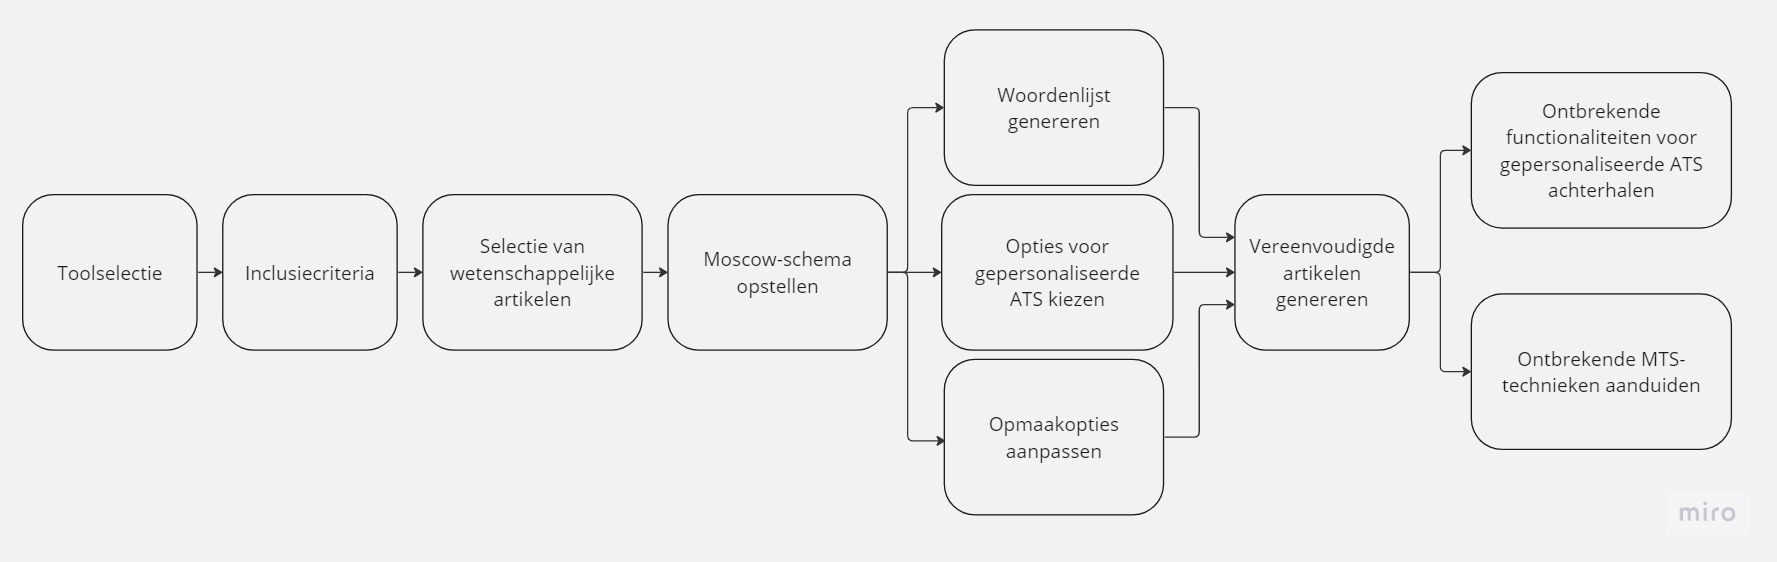
\includegraphics[width=\linewidth]{img/flowchart-requirementsanalyse.jpg}
	\caption{Het benodigde stappenplan bij de requirementanalyse.}
	\label{img:flowchart-requirementsanalyse}
\end{figure}

% TOOLSELECTIE 
Allereerst start het onderzoek met een toolselectie. Zoals aangewezen in sectie \ref{sec:beschikbare-tools-en-taalmodellen}, leent de overheid vijf softwarepakketten uit aan middelbare scholen. Echter neemt de requirementsanalyse drie van deze vijf in de analyse op, want hun functionaliteiten zijn passend voor deze doelgroep. De overige twee zijn minder aanwezig in het onderwijs. Daarnaast toont een zoekopdracht aan dat deze tools geen LS toepassen. Buiten deze erkende softwarepakketten, kunnen online beschikbare tools ook scholieren met dyslexie ondersteunen bij het begrijpend lezen van wetenschappelijke artikelen met ATS, zoals bewezen in \textcite{Bingel2018}. Daarom betrekt de requirementsanalyse enkel tools met onderschreven ATS-functionaliteiten en laat daarmee pure samenvattingstools erbuiten. Tabel \ref{table:shortlist-tools} toont een overzicht van de te experimenteren tools.

\begin{center}
	\begin{table}[H]
		\begin{tabular}{ | m{6cm} | m{6cm} | } 
			\hline
			\textbf{Erkende software} & \textbf{Online beschikbare tools} \\
			\hline
			Sprintplus (E1) & Simplish (O1) \\
			Kurzweil3000 (E2) & SciSpace (O2) \\ 
			AlineaSuite (E3) & Rewordify (O3) \\
			& ChatGPT (O4) \\
			& Bing Chat (O5) \\
			\hline
		\end{tabular}
		\caption{Shortlist van uit te testen tools en toepassingen voor tekstvereenvoudiging.}
		\label{table:shortlist-tools}	
	\end{table}
\end{center}

% Inclusiecritera
Vervolgens bouwt het onderzoek een lijst op van toetsingscriteria. Zo dienen de MTS-technieken uit tabel \ref{table:scientific-paper-struggles} en tabel \ref{table:manual-simplification} als bouwstenen voor het opstellen van de toetsingscriteria. Tabel \ref{table:criteria-requirementsanalysis} geeft een opsomming van de MTS-technieken waaraan tools moeten voldoen. Daarnaast dient dit schema als een inschatting van de functionaliteiten van deze tools.

\begin{center}
	\begin{table}[H]
		\begin{tabular}{ | m{4cm} | m{11cm} | } 
			\hline
			\textbf{MTS-techniek} & \textbf{Functionaliteit} \\
			\hline
			LS & Gepersonaliseerde LS, ofwel woordenschat dat niet te hooggegrepen is. \\
            & Gekende woordenschat mag blijven. \\
			& Woorden met minder lettergrepen gebruiken \\
			& Extra uitleg schrijven bij zinnen \\
			& Paragrafen herschrijven zodat ze eerst uitleg geven op een high-level niveau, vervolgens lagen van complexiteit toevoegen om de lezer te begeleiden \\
			& Woordenlijst aanmaken \\
			& Idiomen vervangen door eenvoudigere synoniemen \\
			\hline
			SS & Zinnen inkorten \\
			& Verwijswoorden aanpassen \\
			& Voorzetseluitdrukkingen aanpassen \\
			& Samengestelde werkwoorden aanpassen \\
			& Actieve stem toepassen \\
			& Enkel regelmatige werkwoorden gebruiken \\
			\hline
			SA & Achtergrondkleur aanpassen \\
			& Woord- en karakterspatiëring \\
			& Consistente lay-out \\
			& Duidelijk zichtbare koppenstructuur \\
			& Huidige positie benadrukken \\
			& Waarschuwingen geven omtrent formulieren en sessies \\
			& Inhoud visueel groeperen \\
			& Tekst herschrijven als tabel \\
			& Tekst herschrijven als opsomming \\
			\hline
		\end{tabular}
		\caption{Richtlijnen waarop het onderzoek de toepassingen aftoetst in de requirementsanalyse.}
		\label{table:criteria-requirementsanalysis}	
	\end{table}
\end{center}

Als realistisch testmateriaal maken de experimenten gebruik van twee gepubliceerde wetenschappelijke artikelen. Zo kunnen deze artikelen relevant zijn voor leerkrachten om aan scholieren in de derde graad van het middelbaar onderwijs te geven als leesvoer. Beide artikelen volgen de kenmerken van een wetenschappelijk artikel, zoals beschreven in tabel \ref{table:scientific-paper-struggles}. Daarnaast gebruiken ze vakjargon en wetenschappelijke concepten in een compact formaat. Tabel \ref{table:referentieteksten-bronvermelding} geeft een overzicht van de twee artikelen en een bijhorende bronvermelding.

\begin{center}
	\begin{table}[H]
		\begin{tabular}{ | m{10cm} | m{5cm} | } 
			\hline
			\textbf{Titel} & \textbf{Bronvermelding} \\
			\hline
			De controle op het gebruik van algoritmische surveillance- onder druk? Een exploratie door de lens van de relationele ethiek & \autocite{VanBrakel2022} \\
			\hline
			Nederland versus België: verschillen in economische dynamiek en beleid. & \autocite{Sleuwaegen2022} \\
			\hline
		\end{tabular}
		\caption{Bronvermeldingen voor de twee wetenschappelijke artikelen.}
		\label{table:referentieteksten-bronvermelding}
	\end{table}
\end{center}

% 4. 
Om een overzicht van de functionaliteiten volgens prioriteit te verkrijgen, bouwt het onderzoek een moscow-schema op vanuit de opgestelde richtlijnen. Zo komen belangrijke functionaliteiten, die nodig zijn om gepersonaliseerde tekstvereenvoudiging met ATS mogelijk te maken, in de categorie \textit{must-haves} terecht. Daarnaast omvatten \textit{should-haves} alle functionaliteiten die niet bijdragen tot gepersonaliseerde ATS, maar wel een meerwaarde biedt in dergelijke toepassingen. Vervolgens bestaan de \textit{could-haves} uit alle functionaliteiten die huidige toepassingen kunnen doen, maar weinig bijdragen tot gepersonaliseerde ATS. Irrelevante functionaliteiten binnen de scope van een prototype of niet toepasselijk voor de doelgroep plaatst het onderzoek als \textit{wont-have}.

\begin{center}
	\begin{table}[H]
		\begin{tabular}{ | m{2cm} | m{13cm} | } 
			\hline
			\textbf{MoSCoW-methode} & \textbf{Functionaliteit} \\
			\hline
			Must-have & Gepersonaliseerde LS, ofwel woordenschat dat niet te hooggegrepen is. Gekende woordenschat mag blijven. \\
			& Woorden met minder lettergrepen gebruiken. \\
			& Woordenlijst aanmaken na handmatige CWI. \\
			& Wetenschappelijke artikelen in PDF-vorm opladen. \\
			& SA-technieken toepassen op de oorspronkelijke tekst. \\
			& Personaliseerbare opmaakopties, waaronder lettertype -en grootte aanpassen, tekstformaat aanpassen, achtergrondkleur aanpassen. \\
			& Duidelijk zichtbare koppenstructuur. \\
			& Tekst herschrijven als opsomming. \\
			\hline
			Should-have & Tekstanalyse \\
			& Extra (in-line) uitleg schrijven bij moeilijke woordenschat. \\
			& Personaliseerbare PDF- of Word-document lay-out. \\
			& Uitvoer als pdf of docx-bestand teruggeven. Het onderzoek gebruikt geen PrintToPDF. \\
			& Wetenschappelijke artikelen in PDF-vorm opladen met OCR. \\
			& Tekstanalyse voor en na de vereenvoudiging aanbieden. \\
			\hline
			Could-have & Huidige positie benadrukken.\\
			& Woordenschat genereren na automatische CWI. \\
			& Waarschuwingen geven omtrent formulieren en sessies. \\
			& Enkel regelmatige werkwoorden gebruiken. \\
			& Extraherende samenvatting \\
			& Abstraherende samenvatting \\
			& Tekst herschrijven in tabelvorm \\
			\hline
			Wont-have & Mobiele versie of \textit{responsive design}. \\
			& Audio-uitvoer \\
			& Integratie met externe toepassingen. Het onderzoek gebruikt Grammarly als voorbeeld voor deze test. \\
			\hline
		\end{tabular}
		\caption{Het moscow-schema voor de requirementsanalyse.}
		\label{img:moscow-table}
	\end{table}
\end{center}

Vervolgens komen experimenten op functionaliteiten voor gepersonaliseerde ATS op wetenschappelijke artikelen aan bod. Allereerst moeten eindgebruikers wetenschappelijke artikelen kunnen opladen. Indien het onderzoek een wetenschappelijk artikel als pdf kan opladen, dan extraheert het de tekstinhoud van het wetenschappelijk artikel. Vervolgens krijgt de toepassing deze tekst als invoer. Zo krijgen de chatbots eerst de prompt, gevolgd door een stuk van het wetenschappelijk artikel. Met zes verschillende prompts kan het onderzoek de LS, SS en SA-functionaliteiten van een promptgebaseerde toepassing achterhalen. Tabel \ref{table:tested-prompts-requirementsanalysis} vermeldt de toegepaste prompts. Toepassingen krijgen eerst een link van het wetenschappelijk artikel. Als de toepassing hier niet over beschikt, dan krijgt de chatbot de tekstinhoud van het wetenschappelijk artikel in \textit{plain-text} mee. 

\begin{center}
	\begin{table}[H]
		\begin{tabular}{ | m{2cm} | m{14cm} | } 
			\hline
			\textbf{Naam} & \textbf{Prompt} \\
			\hline
			P1 & Vereenvoudig deze tekst. \\
			\hline
			P2 & Vereenvoudig deze tekst voor studenten (16-18 jaar) door moeilijke woorden te vervangen, vakjargon te schrappen, woorden langer dan 18 letters te vervangen, acroniemen voluit te schrijven, een woord slechts eenmaal door een synoniem te vervangen, korte uitleg te geven wanneer dat nodig is, en percentages te vervangen. \\
			\hline
			P3 & Vereenvoudig een tekst door deze op te delen in kortere zinnen van maximaal tien woorden. Verander voornaamwoorden als 'zij', 'hun' of 'hij' in namen. Vervang complexe zinsconstructies en voorzetselzinnen door eenvoudiger alternatieven, maar laat ze ongewijzigd als er geen eenvoudiger optie beschikbaar is. \\
			\hline
			P4 & Schrijf de tekst als opsomming. \\
			\hline
			P5 & Schrijf de tekst in tabelformaat. \\
			\hline
			P6 & Genereer op basis van deze tekst een woorden- en synoniemenlijst. \\
			\hline
		\end{tabular}
		\caption{De toegepaste GPT-3-prompts in de requirementsanalyse.}
		\label{table:tested-prompts-requirementsanalysis}
	\end{table}
\end{center}

Daarna voert het onderzoek experimenten uit rond gepersonaliseerde opmaakopties. Kurzweil, SprintPlus en AlineaSuite bieden opmaakopties aan in het instellingenscherm. Zo kunnen eindgebruikers het lettertype, -kleur, -grootte en de achtergrondkleur van de tekst aanpassen naar keuze. Als een toepassing niet over opmaakopties beschikt, stopt het experiment rond opmaakopties voor die toepassing. Tot slot test het onderzoek de mogelijkheden om het formaat van teksten aan te passen met structurele aanpassingen. Zo vragen P4 en P5 specifiek naar een structurele aanpassing, terwijl P1, P2 en P3 minstens een doorlopende tekst als resultaat verwachten. Andere beschikbare tools missen checkboxen of keuzelijsten om deze keuze aan te reiken, waardoor het testen van deze functionaliteit niet mogelijk is.

\section{Vergelijking van taalmodellen}
\label{sec:vergelijkende-studie}

Om wetenschappelijke artikelen met gepersonaliseerde ATS te vereenvoudigen, moet een dergelijk toepassing gebruikmaken van een geschikt taalmodel. Zo moet Pentimentor vereenvoudigde versies van wetenschappelijke artikelen kunnen geven, specifiek volgens de noden van scholieren met dyslexie in de derde graad van het middelbaar onderwijs. Om de uitvoer van het prototype nauwkeurig af te stemmen, moet het onderzoek een antwoord geven op de volgende vraag.

\begin{itemize}
	\item Welk taalmodel kunnen ontwikkelaars inzetten voor tekstvereenvoudiging met ATS van wetenschappelijke artikelen voor scholieren met dyslexie in de derde graad van het middelbaar onderwijs, met dezelfde of gelijkaardige kwaliteiten als gepersonaliseerde tekstvereenvoudiging met MTS?
\end{itemize}

Zoals in de literatuurstudie aangegeven, beschikken ontwikkelaars over onvoldoende gespecialiseerde taalmodellen om wetenschappelijke artikelen te vereenvoudigen. Daarom vergelijkt deze onderzoeksfase alle taalmodellen uit tabel \ref{table:vergelijkende-studie-taalmodellen}. 

\begin{center}
	\begin{table}[H]
		\begin{tabular}{ | m{4cm} | m{11cm} | } 
			\hline
			\textbf{Verwijzing} & \textbf{Taalmodel} \\
			\hline
			T1 & Haining Scientific Abstract Simplification \\
			\hline
			T2 & BART-based Scientific Lay Summarizer \\
			\hline
			T3 & Keep It Simple\\
			\hline
			T4 & GPT-3 \\
			\hline
		\end{tabular}
		\caption{Gebruikte taalmodellen in de vergelijkende studie}
		\label{table:vergelijkende-studie-taalmodellen}
	\end{table}
\end{center}

Deze onderzoeksfase bestaat uit vijf deelfasen, weergegeven op figuur \ref{img:flowchart-vergelijkende-studie-metrics}. Het staat vooral stil bij de vergelijking van leesmetrieken van de oorspronkelijke wetenschappelijke artikelen, MTS-referentieteksten en ATS-teksten. Met een \textit{mixed-methods} onderzoek kan deze onderzoeksfase taalmodellen beoordelen op machinaal en menselijk niveau. Alle scripts kan de lezer terugvinden op de GitHub-repository\footnote{https://github.com/Dyashen/pentimentor/tree/main/bachelorproef/scripts}. Het onderzoek hergebruikt dezelfde wetenschappelijke artikelen als in de requirementsanalyse, namelijk die in tabel \ref{table:referentieteksten-bronvermelding}. Om realistisch referentiemateriaal te verkrijgen, schrijven twee leerkrachten (MTSL) en twee leerlingen zonder dyslexie (MTSL2) zelf een vereenvoudiging van de twee wetenschappelijke artikelen met MTS. Deze vier personen baseren zich op vooraf meegekregen richtlijnen, toegelicht in bijlage \ref{ch:referentietekst}. 

\begin{figure}
	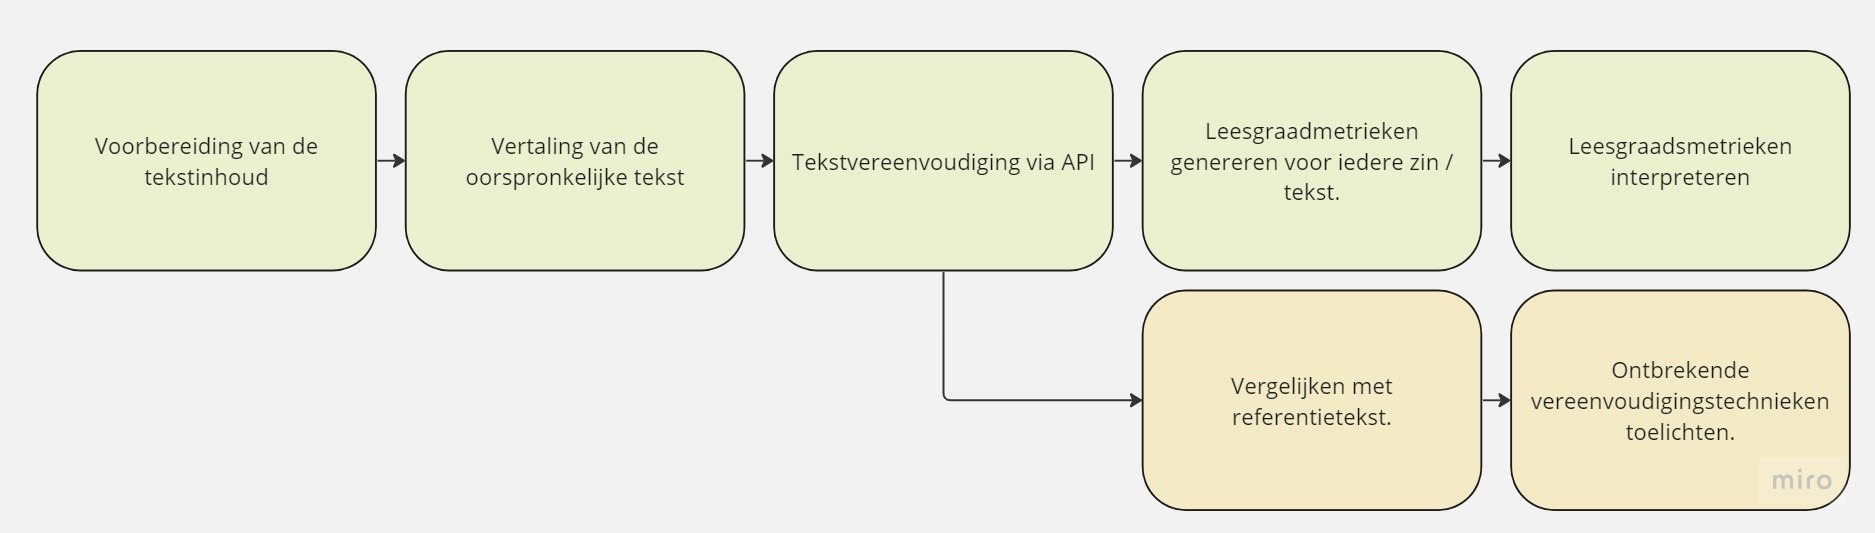
\includegraphics[width=\linewidth]{img/flowchart-vergelijkende-studie.jpg}
	\caption{Het gevolgde stappenplan voor de vergelijking van taalmodellen.}
	\label{img:flowchart-vergelijkende-studie-metrics}
\end{figure}

Allereerst haalt het script de inhoud van de map op met wetenschappelijke artikelen om deze vervolgens in een tekstbestand te plaatsen, zoals weergegeven in codeblok \ref{code:verg-studie-phase-1}. Hier schrijft het script tekstinhoud van het wetenschappelijk artikel over naar een nieuw tekstbestand.

\begin{lstlisting}[language=Python, caption={Script voor de eerste fase van de vergelijkende studie.}, label={code:verg-studie-phase-1}]
def add_newline_after_dot(input_file, output_file):
	with open(input_file, 'r', encoding='utf-8') as file:
		text = file.read()
		text = re.sub(r'\d', '', text)
		modified_text = text.replace('.', '.\n')
		with open(output_file, 'w', encoding='utf-8') as file:
			file.write(modified_text)
		
		folder_path = 'scripts\pdf'
		original_scientific_papers = [f for f in os.listdir(folder_path)]
		
		for paper in original_scientific_papers:
			input_file =  folder_path + '/' + paper
			output_file = folder_path + '/' + 'RE_' + paper
			add_newline_after_dot(input_file, output_file)
\end{lstlisting} 

Vervolgens vertaalt het tweede script alle zinnen naar het Engels. Eerst doorloopt het alle zinnen binnen het wetenschappelijk artikel. Daarna vertaalt het de tekstinhoud met de \textit{deep translator} python-bibliotheek. Als resultaat ontstaat er een csv-bestand met twee kolommen: alle Nederlandstalige en alle Engelstalige zinnen van één wetenschappelijk artikel. Als separator gebruikt het csv-bestand een \textit{pipe}-symbool en zo houdt het rekening met punten en komma's in zinnen.

\begin{center}
	\begin{lstlisting}[language=Python, caption={Script voor de tweede fase van de vergelijkende studie.}, label={code:verg-studie-phase-2}]
def translate_dutch_to_english(dutch_text_file):
	with open(dutch_text_file, 'r', encoding='utf-8') as file:
		dutch_sentences = file.readlines()
		dutch_sentences = [sentence.strip() for sentence in dutch_sentences]
				
		english_sentences = []
		for sentence in dutch_sentences:
			translated = GoogleTranslator(source='nl', target='en').translate(sentence)
			english_sentences.append(translated)
			df = pd.DataFrame({'Dutch': dutch_sentences, 'English': english_sentences})
			df.to_csv(str(dutch_text_file).split('.')[0] + '.csv', index=False)
				
				
		folder_path = 'scripts/pdf/'
		original_scientific_papers = [f for f in os.listdir(folder_path)]
				
		for paper in original_scientific_papers:
			if paper.startswith('RE_') and paper.endswith('.txt'):
				print(f'STARTING {paper}')
				dutch_text_file = folder_path + paper
				translate_dutch_to_english(dutch_text_file)
		\end{lstlisting}
\end{center}

In een derde fase moet het script API-calls voor iedere zin of paragraaf versturen naar ieder taalmodel. Eerst slaat het script een \textit{dictionary} op van taalmodellen om de inhoud van de wetenschappelijke artikelen te vereenvoudigen, zoals weergegeven in listing \ref{code:verg-studie-phase-3}. Daarna vindt tokenisatie plaats, waarvoor het script Spacy \textit{sentence tokenisation} en verwante \textit{embedding models} gebruikt. Deze modellen staan in tabel \ref{table:wordembeddings-spacy}. Na de tokenisatie stuurt het script API-calls naar de hosts van de taalmodellen. Het verzoek naar de \textit{HuggingFace} (HF) API bestaat uit de parameters weergegeven in tabel \ref{table:huggingface-requests-parameters}. Alle HF-taalmodellen vereisen een laadfase. Daarom bevat de \textit{API-call} een extra parameter, namelijk \textit{wait\_for\_model}. Verder past dit script geen extra parameters van de taalmodellen aan. 

\begin{center}
	\begin{table}[H]
		\begin{tabular}{ | m{6cm} | m{8cm} | } 
			\hline
			\textbf{Naam parameter} & \textbf{Waarde} \\
			\hline
			Inputs & De oorspronkelijke zin. Enkel bij T1 komt 'simplify:' voor deze zin. \\
			\hline
			Max length & De lengte van de oorspronkelijke zin + 10 tokens. \\
			\hline
			Wait for model & Altijd ingesteld op \textit{True}. \\
			\hline
		\end{tabular}
		\caption{Meegegeven parameters bij HF-requests}
		\label{table:huggingface-requests-parameters}
	\end{table}
\end{center}

Zoals aangehaald door \textcite{Gooding2022} kunnen promptgebaseerde testen verschillende resultaten leveren, afhankelijk van de gegeven input. Daarom gebruikt het script drie verschillende prompts, gebaseerd op de MTS-technieken beschreven in tabel \ref{table:manual-simplification}. Tabel \ref{table:tested-prompts} visualiseert de gebruikte prompts voor de testen met het GPT-3 model. 

\begin{center}
	\begin{table}[H]
		\begin{tabular}{ | m{2cm} | m{13cm} | } 
			\hline
			\textbf{Naam} & \textbf{Prompt} \\
			\hline
			P1 & Vereenvoudig deze tekst \\
			\hline
			P2 & Vereenvoudig deze tekst voor studenten (16-18 jaar) door moeilijke woorden te vervangen, vakjargon te schrappen, woorden langer dan 18 letters te vervangen, acroniemen voluit te schrijven, een woord slechts eenmaal door een synoniem te vervangen, korte uitleg te geven wanneer dat nodig is, en percentages te vervangen. \\
			\hline
			P3 & Vereenvoudig een tekst door deze op te delen in kortere zinnen van maximaal tien woorden. Verander voornaamwoorden als 'zij', 'hun' of 'hij' in namen. Vervang complexe zinsconstructies en voorzetselzinnen door eenvoudiger alternatieven, maar laat ze ongewijzigd als er geen eenvoudiger optie beschikbaar is. \\
			\hline
		\end{tabular}
		\caption{De GPT-3-prompts die in de vergelijkende studie aan bod komen.}
		\label{table:tested-prompts}
	\end{table}
\end{center}

Zowel T1 als T4 gebruiken een \textit{nul-temperature} en een \textit{top-p} waarde van 90\% om vertrouwde antwoorden te krijgen. Daarnaast dient de top-p om een hoge woordfrequentie te verkrijgen, zoals aangegeven in tabel \ref{table:gpt-3-parameters}. Bij T1 zijn deze twee parameters ingebakken in de functie. Nadien verwerken de taalmodellen iedere zin uit de tekst. Tot slot geeft de HF of GPT-3 API een resultaat in JSON-formaat, bevattende de vereenvoudigde versie van de opgegeven zin. T1, T2 en T3 vereenvoudigen de Engelstalige zinnen, in tegenstelling tot T4 en verwante prompts die de Nederlandstalige zinnen vereenvoudigen. Om een \textit{request failure} door een te lange input te voorkomen, breekt het script de volledige input op per 1000 tokens.

\begin{center}
	\begin{table}[H]
		\begin{tabular}{ | m{7cm} | m{7cm} | } 
			\hline
			\textbf{Taal} & \textbf{Embeddingsmodel} \\
			\hline
			Nederlands & NL Core News Medium \\ 
			\hline
			Engels & EN Core Web Medium \\
			\hline
		\end{tabular}
		\caption{Gebruikte SpaCy word-embeddings}
		\label{table:wordembeddings-spacy}
	\end{table}
\end{center}

\begin{center}
	\begin{lstlisting}[language=Python, caption={Script voor de derde fase van de vergelijkende studie}, label={code:verg-studie-phase-3}]
 def scientific_simplify(self, text, lm_key):
    try:
        API_URL = huggingfacemodels.get(lm_key)
        translated = GoogleTranslator(source='auto', target='en').translate(str(text))
    
        if lm_key == 'T1':
            result = self.query({"inputs": str('simplify: ' + str(translated)),"parameters": {"max_length": len(sentence)+10},"options":{"wait_for_model":True}}, API_URL)
        else:
            result  = self.query({"inputs": str(translated),"parameters": {"max_length": len(sentence)+10},"options":{"wait_for_model":True}}, API_URL)
    
        if 'generated_text' in result[0]:
            translated = GoogleTranslator(source='auto', target='nl').translate(str(result[0]['generated_text']))
            return translated
        elif 'summary_text' in result[0]:
            translated = GoogleTranslator(source='auto', target='nl').translate(str(result[0]['summary_text']))
            return translated
        else:
            return None
        except:
            return text		
            
hf = HuggingFaceModels(os.getenv('huggingface-api-key'))
original_scientific_papers = [f for f in os.listdir(folder_path)]
for paper in original_scientific_papers:
    sentence_tokens = process_file(paper) 
        for sentence in sentence_tokens:
            for model in huggingfacemodels.keys():
                filename = "SIMPLIFIED_"+model+'_'+paper
                with open(filename, 'a', encoding='utf-8') as f:
                    output = hf.scientific_simplify(str(sentence), model)
                    f.write(str(output)) 
	\end{lstlisting}
\end{center}

Vervolgens berekent het script leesmetrieken met de \textit{readability} python-bibliotheek. Leesmetrieken dienen als objectieve maatstaf bij deze vergelijkende studie, zoals aangegeven door \textcite{Nenkova2004}. 

\begin{itemize}
	\item De vergelijkende studie neemt de Flesch-Reading-Ease (FRE) en Gunning FOG (FOG) scores op, want deze scores kunnen de moeilijkheidsgraad van een zin of tekst machinaal meten.
	\item Het aantal complexe en lange woorden kan wijzen op de gebruikte \textit{substitution generation} van het taalmodel. De \textit{Dale-Chall Index} bepaalt de complexiteit van een woord in deze library. Ten slotte tellen alle woorden met meer dan vier lettergrepen mee als een lang woord volgens de \textit{readability}-library.
	\item Het aantal hulpwerkwoorden en vervoegingen van 'zijn' kan aanduiden op mogelijke passieve stem, wat het onderzoek van \textcite{Ruelas2020} als 'hinderende' zinsyntax vernoemt.
\end{itemize}

Dit script resulteert in een \textit{Pandas-dataframe} met alle leesbaarheidsmetrieken uit de \textit{readability}-library. Uiteindelijk slaat het script de \textit{Pandas-dataframe} op als csv-bestand. Listing \ref{code:verg-studie-phase-4} omvat de code voor fase 4. Hierin berekent het script de leesmetrieken voor iedere zin. Allereerst laadt het script twee embeddingsmodellen in, weergegeven in tabel \ref{table:wordembeddings-spacy}. Daarna bouwt het lege dataframes op om de meetresultaten te kunnen opslaan. Vervolgens itereert het python-script door alle tekstbestanden om deze tekst in te lezen. Voor elke zin probeert het script leesmetrieken te verkrijgen met de \textit{readability.getmeasures} functie. Hierbij specifieert het script welke taal de readability-library moet gebruiken. Als het script alle meetwaarden succesvol kan verkrijgen, dan maakt het script een nieuwe rij met machinaal berekende leesmetrieken. Tot slot voegt het alle rijen toe aan de DataFrame. Het script verwerpt de zinnen voor het specifieke artikel waarbij het geen leesmetrieken kan berekenen.

\begin{center}
	\begin{lstlisting}[language=Python, caption={Script voor de vierde fase van de vergelijkende studie}, label={code:verg-studie-phase-4}]	
		simplified_folder = 'scripts/vereenvoudigde_artikelen'
		original_folder = 'scripts/pdf'
		
		scientific_papers = [original_folder + "/" + f for f in os.listdir(original_folder)] + [simplified_folder + "/" + f for f in os.listdir(simplified_folder)]
		
		languages = {
			'nl':'nl_core_news_md',
			'en':'en_core_web_md'
		}
		
		df = pd.DataFrame()
		
		for paper in scientific_papers:
		with open(paper, 'r', encoding='utf-8') as file:
			text = file.read()
			nlp = spacy.load(languages.get('nl'))
			doc = nlp(text)
		
		for sent in doc.sents:
			try:
				metrics = readability.getmeasures(sent.text, lang='nl')
				row = {
					'Paper': paper.split('/')[2].split('.')[0],
					'Sentence': sent.text,
					'FRE': metrics['readability grades']['FleschReadingEase'],
					'FOG': metrics['readability grades']['GunningFogIndex'],
				}
		
		for key, value in metrics['sentence info'].items():
			row[key] = value
		
		for key, value in metrics['word usage'].items():
			row[key] = value
		
		for key, value in metrics['sentence beginnings'].items():
			row[key] = value
			
		df = df.append(row, ignore_index=True)
		except Exception as e:
			print(e)
		
		df.to_csv('result.csv', index=False)
	\end{lstlisting}
\end{center}

In de laatste fase visualiseert het onderzoek de verkregen resultaten. Hierbij gebruikt het \textit{Jupyter-notebooks} en \textit{Matplotlib} om de verkregen resultaten voor te stellen. Allereerst gebruikt de \textit{Jupyter-notebook} een kleinere dataframe met enkel de data van A1. Daarna groepeert het script de data op basis van modellen. Het aantal woorden per zin fungeert als geaggregeerd veld. Met Matplotlib kan het script vervolgens een eenvoudige boxplot genereren. De notebook herhaalt dit proces voor beide artikelen en voor alle leesmetrieken vermeldt in tabel \ref{table:verg-studie-metrieken}. Zo illlustreert \textit{listing} \ref{code:generation-boxplot} hoe het script boxplots genereert. Deze visualiseren het woordgebruik van de verschillende taalmodellen bij A1. Alle code om grafieken te genereren kan de lezer op de GitHub-repository\footnote{https://github.com/dylancluyse/bachelorproef-nlp-tekstvereenvoudiging/blob main/scripts/PHASE\_5.ipynb} terugvinden. 

\begin{lstlisting}[language=Python, caption={Code om een boxplot voor het aantal woorden per zin te genereren.}, label={code:generation-boxplot}]	
artikel_1 = df[(df['paper'] == 'Artikel 1 AI') & (df['FRE'] > 0)]
data = artikel_1.groupby('model')['words_per_sentence']
data_list = [group[1].tolist() for group in data]
plt.figure(figsize=(20,10))
plt.boxplot(data_list)
plt.xticks(range(1, len(data_list) + 1), data.groups.keys())
plt.title('Woorden per zin per model')
plt.xlabel('Model')
plt.ylabel('Woorden per zin')
plt.savefig('boxplot-avg-a1.png')
\end{lstlisting}

Verder toont tabel \ref{table:verg-studie-metrieken} alle leesmetrieken, samen met de toegepaste visualisatietechniek. De boxplots dienen om de spreiding van de leesmetrieken te tonen. Zo kan het onderzoek achterhalen hoe gespreid de gebruikte woordenschat is op het vlak van de leesmetrieken FRE en FOG. De spreiding bij het aantal woorden per zinnen geeft het onderzoek ook weer als een boxplot. Zo kan het onderzoek de regelmaat van korte zinnen achterhalen uit een tekst. De \textit{violinplots} dienen om de verdeling van moeilijke of lange woorden weer te geven. Tot slot maakt het onderzoek gebruik van een staafdiagram om het aantal hulpwerkwoorden of aantal zinnen met een vervoeging van het werkwoord 'zijn' te visualiseren.

\begin{center}
	\begin{table}[H]
		\begin{tabular}{ | m{8cm} | m{7cm} | } 
			\hline
			\textbf{Leesmetriek} & \textbf{Visualisatietechniek }\\
			\hline
			FOG & Boxplot \\
			\hline
			FRE & Boxplot \\
			\hline
			Aantal woorden per zinnen & Boxplot \\
			\hline
			Aantal complexe woorden per zin volgens Dale Chall index & Violinplot \\
			\hline
			Aantal lange woorden per zin & Violinplot \\
			\hline
			Aantal gebruikte hulpwerkwoorden & Staafdiagram \\
			\hline
			Aantal zinnen met een vervoeging van het werkwoord 'zijn' & Staafdiagram \\
			\hline
		\end{tabular}
		\caption{Visualisatietechnieken voor de machinale metrieken bij de vergelijking van de vereenvoudigde teksten met de oorspronkelijke tekst en de referentieteksten.}
		\label{table:verg-studie-metrieken}
	\end{table}
\end{center}

Tenslotte komen de resultaten van de menselijke beoordeling aan bod. Deze fase van de vergelijkende studie staat stil bij aspecten die de leesmetrieken niet kunnen meten, waaronder de normen vermeld in tabel \ref{table:criteria-vergelijkende-studie-human-obv}. De referentietekst dient hier als hulpmiddel om de referentietekst, ofwel het verwachte resultaat, te vergelijken met de vereenvoudigde tekst door een taalmodel. 

\begin{table}[H]
	\begin{tabular}{| m{10cm} | m{4.5cm} |}
		\hline
		\textbf{Metriek} & \textbf{Vereenvoudigings- techniek} \\ \hline
		Acroniemen behouden & LS 	\\ \hline
		Inschatting van de doelgroep & LS	\\ \hline
		Behoud van kern- en bijzaken & LS \\ \hline
		Schrijven in tabelvorm of als opsomming & SA \\ \hline
		Passieve zinconstructies herschrijven naar actieve zinconstructies & SS \\ \hline
		Bronvermelding behouden &  SA \\ \hline
		Citeren en parafraseren & SS en SA. \\ \hline
	\end{tabular}
	\caption{Criteria voor menselijke observatie bij de vergelijkende studie.}
	\label{table:criteria-vergelijkende-studie-human-obv}
\end{table}

\section{Prototype voor tekstvereenvoudiging}

Met de gevonden vereisten voor een taalmodel uit het moscow-schema en de geschikte taalmodellen voor gepersonaliseerde ATS kan het onderzoek een volgende stap zetten om de onderzoeksvraag te beantwoorden. De volgende sectie omschrijft de ontwikkeling van Pentimentor, namelijk een prototype voor gepersonaliseerde ATS voor scholieren met dyslexie in de derde graad van het middelbaar onderwijs. Deze ontwikkeling kan ontwikkelaars helpen als rode draad bij het maken van dergelijke toepassingen. Zo beantwoordt de ontwikkeling van \textit{Pentimentor} volgende deelvraag: 

\begin{itemize}
	\item Hoe kunnen ontwikkelaars een intuïtieve en lokale webtoepassing ontwikkelen die zowel scholieren met dyslexie als leerkrachten kan helpen bij het vereenvoudigen van wetenschappelijke artikelen met behoud van semantiek, jargon en zinsstructuren?
\end{itemize}

Voor de ontwikkeling van het prototype volgt het onderzoek figuur \ref{img:general-overview-prototype}. Deze flowchart toont zes algemene fasen. Zo start het onderzoek met een voorbereidende fase waarin het onderzoek de nodige technieken en taalmodellen opsomt. Vervolgens ontwikkelt het de backend en frontend. Daarna ontwikkelt het twee algemene componenten: een leraren -en scholierencomponent. Hierna moet het onderzoek stilstaan bij de opzet van Pentimentor. 

\medspace

Uiteindelijk beoordeelt het onderzoek de \textit{Pentimentor} prototype. Het vergelijkt dit met andere toepassingen volgens het moscow-schema. Zo moet het lerarencomponent wetenschappelijke artikelen kunnen vereenvoudigen, nadat de gebruiker ATS-technieken selecteert. Daarnaast moet het scholierencomponent ondersteuning bieden aan scholieren die de verschillen tussen de originele en vereenvoudigde tekst willen zien. Hier moeten scholieren met dyslexie in \textit{real-time} aanpassingen kunnen maken aan de tekst en ondersteuning krijgen tijdens het begrijpend lezen van een tekst. Tot slot moeten gepersonaliseerde opmaakopties gelijk blijven over alle pagina's heen van Pentimentor.


\begin{sidewaysfigure}
	\begin{figure}[H]
		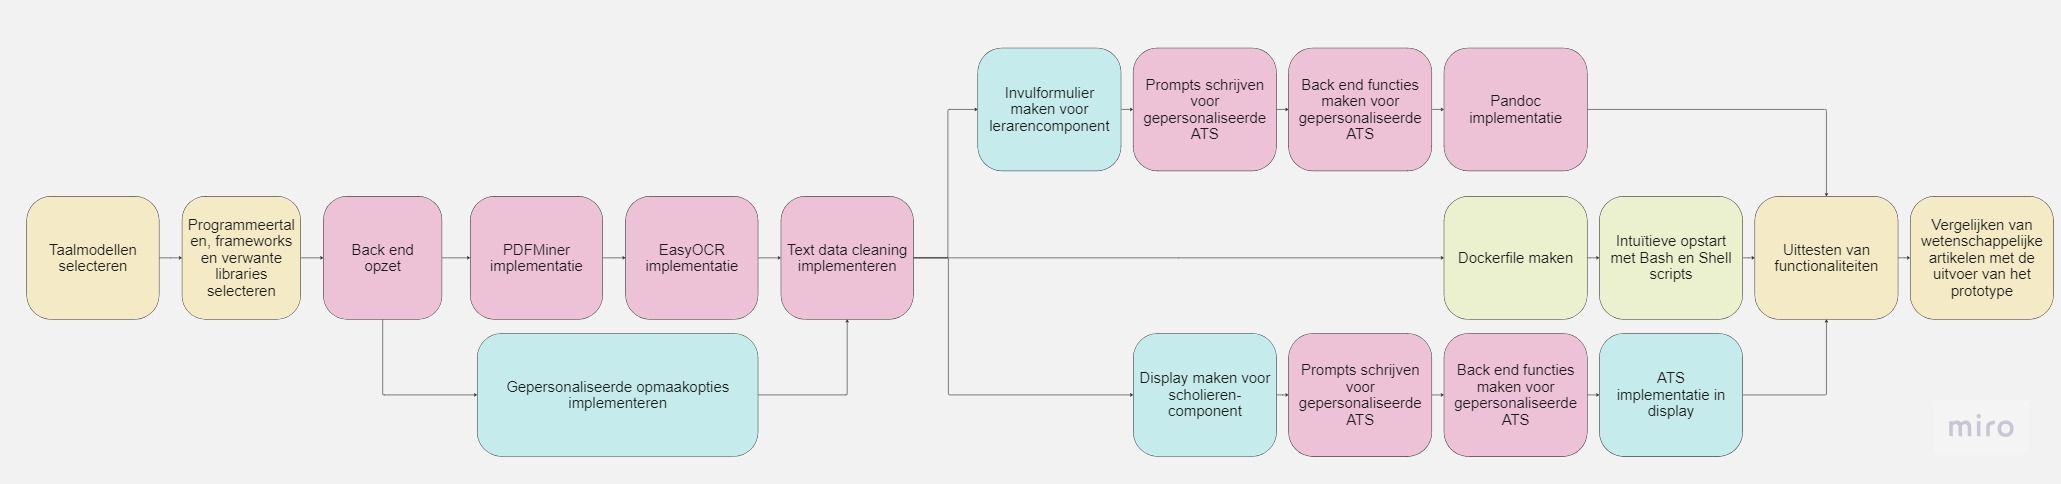
\includegraphics[width=\linewidth]{img/flowchart-general-development.jpg}
		\caption{Algemeen overzicht van de ontwikkeling van het prototype voor ATS van wetenschappelijke artikelen.}
		\label{img:general-overview-prototype}
	\end{figure}
\end{sidewaysfigure}

\subsubsection{Taalmodellen selecteren}

Omdat de keuze van taalmodellen verdere technologiekeuzes kan beïnvloeden, bepaalt het onderzoek eerst één of meerdere taalmodellen voor gepersonaliseerde ATS. Zo wijst de vorige onderzoeksfase uit dat GPT-3 een geschikt taalmodel is voor gepersonaliseerde ATS. Voor een abstraherende samenvatting kan \textit{Pentimentor} één van drie taalmodellen uit de vorige onderzoeksfase gebruiken.

\subsubsection{Programmeertalen, frameworks en verwante libraries selecteren}

Voor een snelle en gratis ontwikkeling gebruikt \textit{Pentimentor} \textit{open-source} pakketten. Taalmodellen kunnen het aanspreken via \textit{API-calls} met JS of Python. Omdat het systeem de API-sleutel moet opslaan als sessievariabele, gebeuren alle \textit{API-calls} vanuit de backend. Verder vermeldt tabel \ref{table:technologies} alle gebruikte programmeertalen. Tot slot vermeldt tabel \ref{table:python-libraries} alle gebruikte python-libraries.

\begin{center}
	\begin{table}[H]
	\begin{tabular}{ | m{4cm} | m{11cm} | } 
		\hline
		\textbf{Technologie} 	& \textbf{Functionaliteit} \\
		\hline
		Python 					& Dit dient voor de backend die API-calls en PoS-tags verwerkt. \\
		\hline
		JavaScript (JS)			& Dit maakt de toepassing eenduidig door CLI-instructies te vervangen door knoppen. \\
		\hline
		HTML en CSS 			& Dit past het uiterlijk aan, naargelang de gekozen parameters van de eindgebruiker. \\
		\hline
		Jinja 					& Dit geeft alle Python backend data door aan de frontend.  \\
		\hline
		Docker 					& Dit dient om Pentimentor lokaal op te kunnen starten en voorziet een lokale omgeving waarin het systeem alle software installeert. \\
		\hline
		Bash					& Script om de lokale opzet op eenduidige wijze op te starten voor Linux en Mac-systemen. \\
		\hline
		Powershell 				& Script om de lokale opzet op eenduidige wijze op te starten voor Windows-systemen. \\
		\hline
	\end{tabular}
	\caption{Gebruikte programmeertalen in het prototype voor tekstvereenvoudiging.}
	\label{table:technologies}
	\end{table}
\end{center}

\begin{center}
	\begin{table}[H]
	\begin{tabular}{ | m{4cm} | m{11cm} | } 
		\hline
		\textbf{Python-bibliotheek} & \textbf{Functionaliteit} \\
		\hline
		Flask					& Het websiteframework van Pentimentor. Dit framework combineert frontend en backend. \\ 
		\hline
		PDFMiner 				& Tekstinhoud van PDF's extraheren. \\ 
		\hline
		LayoutParser			& Selectief tekstinhoud uit PDF's extraheren. \\
		\hline
		NumPy 					& De \textit{reshape}-functie vereenvoudigt de ontwikkeling om dynamisch paragrafen uit te printen. \\
		\hline		
		Spacy 					& \textit{PoS-tagging} en \textit{token lemmatization}. \\
		\hline
		OpenAI					& GPT-3 API aanspreken. \\
		\hline
	\end{tabular}
	\caption{Gebruikte Python-libraries en hun respectievelijke functie in het prototype.}
	\label{table:python-libraries}
	\end{table}
\end{center}

\subsubsection{Backend opzet}

Nadat het onderzoek taalmodellen, technologieën en frameworks uitkiest, start het met de frontend implementatie. Allereerst voegt het de homepagina toe. Dit dient als portaal voor de componenten. Daarna implementeert het personaliseerbare opmaakopties. Zoals aangeraden door \textcite{Galliussi2020}, moeten ontwikkelaars hiermee rekening houden. Zo gebruikt Pentimentor parameters onderzocht door \textcite{Rello2013a, Rello2013b}. Om deze instellingen aan te bieden, voegt het onderzoek een webpagina toe. Deze HTML-pagina bevat formulieren met aanpasbare parameters. Nadat de gebruiker parameters aanpast, stuurt de pagina een POST-request naar de backend. Het verwerkt dit en slaat de ontvangen dictionary op als sessievariabele, zoals weergegeven in listing \ref{code:back-end-session-personalized}. Tot slot laadt de frontend deze opmaakopties in bij iedere wegpagina. Dit gebeurt met \textit{window onload}, zoals weergegeven in listing \ref{code:window-onload-js}. Zo hoeven eindgebruikers deze parameters niet bij iedere webpagina opnieuw aan te passen.


\begin{lstlisting}[language=python, caption={De backend functie die de aanpassingen uit het formulier opslaat als sessievariabele.}, label={code:back-end-session-personalized}]
PER_SET_SESSION_NAME = 'personalized_settings'

@app.route('/get-settings-user',methods=['POST'])
def return_personal_settings_dict():
	if PER_SET_SESSION_NAME in session:
		return jsonify(session[PER_SET_SESSION_NAME])
	else:
		return jsonify(result='session does not exist')
	
@app.route('/change-settings-user', methods=['POST'])
def change_personal_settings():
	try:
		session[PER_SET_SESSION_NAME] = dict(request.form)
		msg = 'Succesvol aangepast!'
	except Exception as e:
		msg = str(e)
		flash(msg)
	return render_template('settings.html')
\end{lstlisting}

\begin{lstlisting}[language=javascript, caption={De onload-functie die de gepersonaliseerde opmaakopties regelt bij het inladen van een webpagina.}, label={code:window-onload-js}]
window.onload = async function () {
	var url = `http://localhost:5000/get-settings-user`;
	const response = await fetch(url, { method: 'POST' });
	var result = await response.json();
	document.body.style.fontSize        = result.fontSize+'px';
	document.body.style.fontFamily      = result.fontSettings;
	document.body.style.backgroundColor = result.favcolor;
	document.body.style.lineHeight      = result.lineHeight+'cm';
	document.body.style.wordSpacing     = result.wordSpacing+'cm';
	document.body.style.textAlign       = result.textAlign;
}
\end{lstlisting}

Naast personaliseerbare opmaakopties moet \textit{Pentimentor} wetenschappelijke artikelen kunnen inladen en inlezen. Zo kan het met \textit{PDF-extractors} zoals \textit{PDFMiner} tekst uit de PDF extraheren. Niet alle \textit{PDF-extractors} zijn foutbestendig, want zoals opgemerkt in de literatuurstudie kunnen \textit{PDF-extractors} ook tekst verliezen tijdens dit proces. Om dit te voorkomen, biedt het prototype een OCR-optie met \textit{LayoutParser} aan. Beide manieren vereisen functies in de backend en frontend.

\medspace

Aan de frontend voegt het onderzoek checkboxes, file-input en texarea-input tags toe. Uiteindelijk stuurt het formulier een POST-request om alle meegekregen informatie door te sturen naar de backend. Na het ontvangen van de request van de frontend, handelt de Flask backend het bestand verder af zoals aangewezen in listing \ref{code:inlezen-wetenschappelijk-artikel-front-end-back-end}. Nadat de gebruiker het formulier bevestigt, geeft het de binaries van het wetenschappelijk artikel door aan de backend. Die controleert het type invoer en slaat het nadien tijdelijk \textit{in-memory} op. Daarnaast krijgt het de keuze tussen normale of OCR-upload mee als boolean, waarbij \textit{true} gelijk staat aan een afhandeling met LayoutParser.

\begin{lstlisting}[language=Python, caption={Koppeling tussen frontend en backend voor het inlezen van een wetenschappelijk artikel}, label={code:inlezen-wetenschappelijk-artikel-front-end-back-end}]
def setup_scholars_teachers(request):
	settings = request.form
	if 'fullText' in request.form:
		text = request.form['fullText']
		langs = detect_langs(text)
		reader = Reader()
		dict_text = reader.get_full_text_site(text)                
	elif 'pdf' in request.files:
		if 'advanced' not in settings:
			pdf = request.files['pdf']
			pdf_data = BytesIO(pdf.read())
			all_pages = extract_pages(pdf_data,page_numbers=None,maxpages=999)
			langs = detect_langs(str(all_pages))
			reader = Reader()
			full_text = reader.get_full_text_dict(all_pages)
			dict_text = reader.get_full_text_site(full_text)
		else:
			pdf = request.files['pdf']
			pdf_data = pdf.read()
			pages = convert_from_bytes(pdf_data)
			reader = Reader()
			img_text = reader.get_full_text_from_image(pages)
			langs = detect_langs(img_text)
			dict_text = reader.get_full_text_site(img_text)                            
			return dict_text, langs, 'voorbeeldtitel', 'voorbeeldonderwerp'
			
@app.route('/for-scholars', methods=['GET','POST'])
def teaching_tool():
	try:
		dict_text, langs, title, subject = setup_scholars_teachers(request)
		return render_template('for-scholars.html', pdf=dict_text, lang=langs, title=title, subject=subject)
	except Exception as e:
		return render_template('error.html',error=str(e))
	
@app.route('/for-teachers', methods=['GET','POST'])
def analysing_choosing_for_teachers():
	try:
		dict_text, langs, title, subject = setup_scholars_teachers(request)
		return render_template('for-teachers.html', pdf=dict_text, lang=langs, title=title, subject=subject)
	except Exception as e:
		return render_template('error.html',error=str(e))
\end{lstlisting}

\subsubsection{PDFMiner implementatie}

Bij een gewone PDF-extractie gebruikt de Reader-klasse PDFMiner met de functie in listing \ref{code:inlezen-van-pdf}. Het itereert door alle pagina's van een opgeladen wetenschappelijk artikel. Nadien extraheert het alle tekst van een pagina en concateneert het alle opgehaalde tekst van één pagina aan een lege string. Dit proces herhaalt zich tot het geen pagina's meer kan inlezen. Tot slot resulteert dit in een string-object met alle geëxtraheerde tekst uit het wetenschappelijk artikel. Hierna moet de Reader-klasse deze tekst formatteren tot een leesbaar formaat.

\begin{lstlisting}[language=Python, caption={Een PDF inlezen met PDFMiner}, label={code:inlezen-van-pdf}]
	def get_full_text_from_pdf(self, all_pages):
		total = ""
		for page_layout in all_pages:
			for element in page_layout:
				if isinstance(element, LTTextContainer):
				for text_line in element:
					total += text_line.get_text()
					return total
\end{lstlisting}

\subsubsection{OCR implementatie}

Tekst kan ontbreken na het extraheerproces met PDFMiner. Daarnaast krijgt Pentimentor als resultaat één string van alle karakters. Tot gevolg toont het deze tekst op een niet-georganiseerde manier. Daarom voorziet het prototype een tweede methode met OCR en machineleertechnieken (ML). Zo gebruikt Pentimentor het Python-pakket \textit{Layoutparser} om bovenstaand probleem op te lossen.

\medspace

In eerste instantie moet de backend alle pagina's omzetten naar een machine-interpreteerbaar formaat door ze eerst om te zetten naar afbeeldingen en vervolgens naar binaire waarden. Met behulp van LayoutParser en het Detectron2-algoritme kan Pentimentor de verschillende tekstonderdelen op elke pagina classificeren, waaronder tekst-, titel-, figuur- en tabelblokken. Omdat figuren en tabellen niet relevant zijn voor dit onderzoek, concentreert Pentimentor zich op het achterhalen van titels en tekst. Die slaat het systeem op in een array genaamd 'valid'. Daarna omkadert LayoutParser alle tekstblokken en koppelt het elk tekstblok met een unieke id-tag. Listing \ref{listing:reader-ocr} illustreert het proces om de blokken op één pagina te achterhalen.

\begin{lstlisting}[language=Python, caption={Een PDF inlezen met OCR}, label={listing:reader-ocr}]
model = lp.Detectron2LayoutModel(
	config_path ='lp://PubLayNet/faster_rcnn_R_50_FPN_3x/config',
	label_map   ={0: "Text", 1: "Title", 2: "List", 3:"Table", 4:"Figure"}, 
	extra_config=["MODEL.ROI_HEADS.SCORE_THRESH_TEST", 0.8])

image = cv2.imread(img_folder + afbeelding)
image = image[..., ::-1]
	
layout = model.detect(image)
	
lp.draw_box(image, layout, box_width=3)
	
valid = ['Text', 'Title']
text_blocks = lp.Layout([b for b in layout if b.type in valid])
	
h, w = image.shape[:2]
	
left_interval = lp.Interval(0, w/2*1.05, axis='x').put_on_canvas(image)
	
left_blocks = text_blocks.filter_by(left_interval, center=True)
left_blocks.sort(key=lambda b:b.coordinates[1], inplace=True)
	
right_blocks = [b for b in text_blocks if b not in left_blocks]
right_blocks.sort(key=lambda b:b.coordinates[1])
	
text_blocks = lp.Layout([b.set(id=idx) for idx, b in enumerate(left_blocks+right_blocks)])
	
lp.draw_box(image, text_blocks, box_width=3, show_element_id=True)
	
\end{lstlisting}

Nu beschikt Pentimentor over een array van afbeeldingen. Vervolgens moet het alle tekst uit deze blokken kunnen extraheren. Hiervoor raadt de documentatie van Layoutparser een OCR-methode aan. Listing \ref{listing:text-collecting} illustreert dit. Zo gebruikt Pentimentor de Python-bibliotheek \textit{Tesseract} om de titels en tekst te extraheren uit de afbeeldingen. Omdat het systeem niet bijhoudt wat titel of tekstblok is, voegt het systeem een string toe aan iedere tekstblok. Zo resulteert deze functie in een array met alle teruggevonden titel- en tekstblokken.

\begin{lstlisting}[language=Python, caption={Tekst extraheren uit de geparsete inhoud.}, label={listing:text-collecting}]
language = language
ocr_agent = lp.TesseractAgent(languages=language)

full_text = []
	
for block in text_blocks:
	segment_image = (block.pad(left=5, right=5, top=5, bottom=5).crop_image(image))
	text          = ocr_agent.detect(segment_image)
	block.set(text=text, inplace=True)
	
for t in text_blocks:
	if(t.type == 'Title'):
		full_text.append('title:' + str(t.text))
	else:
		full_text.append(t.text)    
	return full_text
    
\end{lstlisting}

\subsubsection{Geëxtraheerde inhoud formatteren naar een webpagina.}

Na het extraheren van tekst volgt het formatteren ervan. Hier zet het systeem de tekst om naar het gewenste formaat voor de \textit{frontend}. In eerste instantie transformeert de \textit{backend} de geëxtraheerde tekst naar \textit{arrays} van zinnen met behulp van Spacy \textit{word embeddings} en \textit{sentence embeddings}. Listing \ref{code:reader-formatting} illustreert de werking van deze techniek. Zo bundelt de backend een parameteriseerbaar aanal zinnen met behulp van \textit{Numpy reshape}. Om de Part-of-Speech (PoS)-tag bij het respectievelijke woorde te behouden, gebruikt de backend een sleutelpaarstructuur. Elke sleutel verwijst naar een woord in een zin, terwijl de waarde naar de bijbehorende PoS-tag verwijst. Het onderzoek focust zich op de ontwikkeling voor de vereenvoudiging van Nederlandstalige of Engelstalige wetenschappelijke artikelen. Daarom laadt Pentimentor hoogstens twee embeddingsmodellen in. Tabel \ref{table:wordembeddings-spacy} vermeldt deze embeddingsmodellen. Standaard maakt Pentimentor gebruik van een Engelstalig embeddingsmodel als de backend de taal niet kan herkennen of als de taal niet voorkomt in een \textit{dictionary}. 

\begin{lstlisting}[language=Python, caption={Het formatteren van de tekst naar een formaat voor de website.}, label={code:reader-formatting}]
	def get_full_text_site(self, full_text):
		try:
			lang = detect(full_text)
		except:
			lang = 'en'
		
		if lang in dict:
			nlp = spacy.load(dict.get(lang))
		else:
			nlp = spacy.load(dict.get('en'))
		
		full_text = str(full_text).replace('\n', ' ')
		
		doc = nlp(full_text)
		sentences = []
		for sentence in doc.sents:
			sentences.append(sentence)
		
		pad_size = SENTENCES_PER_PARAGRAPH - (len(sentences) % SENTENCES_PER_PARAGRAPH)
		padded_a = np.pad(sentences, (0, pad_size), mode='empty')
		paragraphs = padded_a.reshape(-1, SENTENCES_PER_PARAGRAPH)
		
		text_w_pos = []
		for paragraph in paragraphs:
			paragraph_w_pos = []
			try:
				for sentence in paragraph:
				dict_sentence = {}
				for token in sentence:
					dict_sentence[token.text] = str(token.pos_).lower()
					paragraph_w_pos.append(dict_sentence)    
					text_w_pos.append(paragraph_w_pos)
			except:
				pass
				
		return text_w_pos
\end{lstlisting}

Beide componenten moeten het artikel in een aangepaste pagina tonen. Daarom maakt deze fase gebruik van Jinja2, de \textit{templating engine} van Flask. Hiermee kan de frontend de array uit de vorige fase itereren en vervolgens uitprinten. Ieder woord koppelt de backend met een PoS-tag. Daarom koppelt de frontend iedere zin met de overkoepelende span-tag \textit{sentence}. Daarna koppelt het ieder woord met de klasse \textit{nouns}, \textit{adjectives} of \textit{verbs}. Andere woorden, zoals conjuncties, koppelt het systeem met de klasse \textit{other}.

\begin{lstlisting}[language=html, caption={Het doorlopen van de PDF-tekst op de webpagina en het toekennen van de span-tags.}, label={code:html-span-tags}]

	<p class="left-side">
		
		<span class="sentence">
			
			
			<span class={{sentence[word]}}>{{word}}</span>
			
			
		</span>
	
	</p>

\end{lstlisting}


\subsubsection{Invulformulier maken voor het lerarencomponent.}

Zo kunnen leerkrachten beschikken over een tool waarin zij de geëxtraheerde tekstinhoud kunnen manipuleren, om vervolgens opties voor gepersonaliseerde ATS te selecteren. Figuur \ref{img:proto-lerarencomponent} toont een mogelijke weergave van deze HTML-pagina. Leerkrachten moeten in dit lerarencomponent kunnen beschikken over de functionaliteiten weergegeven in tabel \ref{table:functionaliteiten-leerkrachten}. Tabel \ref{table:criteria-requirementsanalysis} reikt de benodigde opties voor gepersonaliseerde ATS aan. Het prototype gebruikt deze criteria als opties om de prompts dynamisch op te bouwen.

\begin{center}
	\begin{table}[H]
		\begin{tabular}{ | m{7cm} | m{8cm} | } 
			\hline
			\textbf{Functionaliteit} & Gebruikte JS of python-techniek \\
			\hline
			Specifieke prompt meegeven per paragraaf & Naast een optie om voor het hele document één prompt te gebruiken, voegt het prototype ook een optie toe om. Hiervoor past de webinhoud sleutelparen toe. \\
			\hline
			Opties voor gepersonaliseerde ATS aanreiken. & Met behulp van een HTML-formulier kunnen leerkrachten opties aanvinken waaraan de vereenvoudigde tekst moet voldoen. \\
			\hline
			Werkwoorden, bijvoeglijke en zelfstandige naamwoorden markeren & Frontend aanpassing met \textit{eventlistener}. De tekstkleur van het aangeduide type woorden verandert naar het gekozen kleur. \\
			\hline
			Zinnen verwijderen & \textit{Frontend} filter aangesproken door een \textit{eventlistener}. \\
			\hline
			Woord toevoegen aan de woordenlijst & Een \textit{eventlistener} handelt de functionaliteit af. Het prototype slaat woorden en hun context tijdelijk op. Het formulier houdt dit bij en geeft het vervolgens mee bij het indienen. Deze woorden en hun respectievelijke zin van voorkomen dienen om de woordenlijst op te vullen in het gegenereerde PDF of Word-bestand. \\ 
			\hline 
		\end{tabular}
	\caption{Alle beschikbare functionaliteiten in het lerarencomponent.}
	\label{table:functionaliteiten-leerkrachten}
	\end{table}
\end{center}

\subsubsection{Prompts schrijven voor gepersonaliseerde ATS in het lerarencomponent}

Het onderzoek stelt de prompts op volgens de richtlijnen beschreven in tabel \ref{table:techniques-for-good-prompts}. Daarnaast past het Intent- en Contextualization prompts toe zoals aangeraden door \textcite{White2023}. Tabel \ref{table:prompts-lerarencomponent} geeft een overzicht van alle opgestelde prompts die het prototype gebruikt in het lerarencomponent. Daarnaast gebruikt iedere API-call de parameters omschreven in tabel \ref{table:gpt-3-parameters-lerarencomponent}.

\begin{center}
	
\end{center}
\begin{table}[H]
	\begin{tabular}{ | m{5cm} | m{10cm} |}
		\hline
		\textbf{Functionaliteit} & \textbf{Prompt} \\ \hline
		Synoniem opzoeken & Geef een eenvoudiger synoniem voor '{woord}'. Context {context}. \\ \hline
		Definitie opzoeken & Geef een eenvoudige definitie voor '{woord}'. Context {context}.\\ \hline
		Zin vereenvoudigen & Schrijf deze zin eenvoudiger // '{zin}'\\ \hline
		Gepersonaliseerde ATS & Schrijf deze zin eenvoudiger volgens de colgende criteria // '{zin}' // criteria: '{criteria}'\\ \hline
		Gepersonaliseerde ATS als opsomming & Herschrijf dit als een lijst van vereenvoudigde zinnen met (gepersonaliseerde opties) :return: een lijst van vereenvoudigde zinnen gesplitst door een '|' teken /// {context}\\ \hline
	\end{tabular}
	\caption{Tabel met de gebruikte prompts voor het lerarencomponent.}
	\label{table:prompts-lerarencomponent}
\end{table}

\begin{center}
	\begin{table}[H]
		\begin{tabular}{| m{5cm}| m{10cm} |}
			\hline
			\textbf{Parameter} & \textbf{Gebruikte waarde} \\ \hline
			Prompt & Zie tabel \ref{table:prompts-lerarencomponent} \\ \hline
			Temperature & 0 \\ \hline
			Max tokens & De lengte van het woord vermeerdert met tien tokens als het over het opzoeken van een definitie of synoniem gaat. \\ 
			& Of de lengte van de zin vermeerdert met twintig tokens indien het over vereenvoudiging van een zin gaat. \\
			\hline
			Model & Da Vinci 3 \\ \hline
			Top-p & 90\% \\ \hline
			Stream & False \\ \hline
		\end{tabular}
		\caption{Gebruikte parameters om definities van woorden te genereren met GPT-3.}
		\label{table:gpt-3-parameters-lerarencomponent}
	\end{table}
\end{center}


\subsubsection{Functies voor gepersonaliseerde ATS in het lerarencomponent}

Gebruikers kunnen Pentimentor op twee manieren gebruiken. Zij kunnen het volledige artikel automatisch laten vereenvoudigen of samenvatten, of specifiek fragmenten markeren om een gepersonaliseerde vereenvoudiging of samenvatting te laten maken. Zo moet Pentimentor een nieuwe doorlopende tekst kunnen genereren, als opsomming of tabel laten herschrijven of woordenlijsten genereren. Hiervoor moet het twee zaken bijhouden: de gemarkeerde tekst en de optie die de gebruiker wenst te kiezen. Hiervoor gebruikt het onderzoek een sleutelpaarstructuur. Zo biedt \textit{localstorage} een tijdelijk persistente methode. De frontend moet de \textit{localstorage} opvullen met gemarkeerde tekst en na gebruik opnieuw leegmaken. Als het systeem dit niet leegmaakt, dan neemt het systeem overblijfselen van vorige artikelen over. Om eindgebruikers van hun keuzes bewust te maken, markeert de frontend deze tekst met een kleur. Verder maakt de frontend de eindgebruiker bewust welke kleur bij welke transformatie hoort. Tot slot toont listing \ref{listing:localstorage} de werking van deze methode.

\begin{lstlisting}[language=javascript, caption={Implementatie rond localstorage en tekst markeren.}, label={listing:localstorage}]
function addTextWithParagraph() {
	text = window.getSelection().toString();
	if (text == "") {
		return;
	} else {
		var fieldset = document.querySelector(".personalized");
		var inputs = fieldset.querySelectorAll("input");
		var values = [];
		for (var i = 0; i < inputs.length; i++) {
			if (inputs[i].type === "checkbox" && inputs[i].checked) {
				values.push(inputs[i].value);
			}
		}
		
		var selection = window.getSelection();
		if (selection.rangeCount > 0) {
			var range = selection.getRangeAt(0);
			var commonAncestor = range.commonAncestorContainer;
			var selectedElements = commonAncestor.getElementsByClassName("sentence");
			var selectedTags = [];
			for (var i = 0; i < selectedElements.length; i++) {
				var elementRange = document.createRange();
				elementRange.selectNodeContents(selectedElements[i]);
				
				if (range.intersectsNode(selectedElements[i])) {
					selectedTags.push(selectedElements[i]);
				}
			}
		}
		
		fullText = "";
		
		for (var i = 0; i < selectedTags.length; i++) {
			var tag = selectedTags[i];
			if (values.includes('summation')) {
				tag.style.backgroundColor = "#F0FFF0";
			} else if (values.includes('glossary')){
				tag.style.backgroundColor = "#F5DEB3";
			} else if (values.includes('table')) {
				tag.style.backgroundColor = "#FAFAD2";
			} else {
				tag.style.backgroundColor = "#F5F5DC";
			}
			
			var tagText = tag.textContent;
			tagText = tagText.split('\n').join('').replace(/:/g, "");
			fullText += tagText;
		}
		localStorage.setItem(fullText, values);
	}
}

function getAllLocalStorageValues() {
	var localStorageValues = {};
	for (var i = 0; i < localStorage.length; i++) {
		var key = localStorage.key(i);
		var value = localStorage.getItem(key);
		localStorageValues[key] = value;
	}
	return localStorageValues;
}
\end{lstlisting}

\subsubsection{Verbinding met GPT-3}

Om de gemarkeerde tekst te kunnen verwerken, moet het systeem de inhoud van de \textit{localstorage} doorsturen naar de backend. Vervolgens moet het ieder sleutelpaar overlopen. Iedere sleutel stelt een fragment voor dat de backend moet vereenvoudigen of samenvatten. Als de tekst het maximum aantal tokens overschrijdt, splitst de backend deze tekst op in een aantal delen dat gelijk staat aan de gelijke deling van het maximum aantal tokens, zoals weergegeven in listing \ref{code:localstorage-iteration}.

\begin{lstlisting}[language=Python, caption={Alle gemarkeerde tekstblokken uit de localstorage aflopen en doorsturen naar het markdown document.}, label={code:localstorage-iteration}]
for key, value in full_text.items():
	new_sentence = []
	for word in key.split(" "):
		if word != '':
			new_sentence.append(word)
	sent            = " ".join(new_sentence)
	aantalDelingen  = (len(sent)  // 1000) + 1
	perHoeveel      = (len(sent)) // aantalDelingen
	sent = [sent[i:i+perHoeveel] for i in range(0, len(sent), perHoeveel)]
	
	for s in sent:
		new_sent, prompt = gpt.personalised_simplify(s, str(value).split(','))
		if 'summation' in str(value).split(','):
			doc_creator.generate_summary_w_summation(new_sent)
		elif 'table' in str(value).split(',') or 'glossary' in str(value).split(','):
			doc_creator.generate_simplification(new_sent)
		else:
			doc_creator.generate_simplification(new_sent)
\end{lstlisting}

Vervolgens moet de \textit{backend} deze prompts naar de GPT-3 API sturen. Zo itereert het over ieder sleutelpaar en bouwt het daarmee prompts op. Deze bestaat uit gekozen opties en gemarkeerde tekst van de gebruiker. Naast de prompt dient de backend ook parameters mee te geven. Deze omvatten alle waarden opgelijst in tabel \ref{table:gpt-3-parameters-lerarencomponent}. Omdat formaatwijzigingen specifieke prompts vereisen, bestaat de prompt uit extra klemtonen om het resultaat in markdowncode terug te krijgen. Als de \textit{backend} geen formaatwijziging moet uitvoeren, dan stuurt het generieke prompts met daarin een opsomming van alle kenmerken die de eindgebruiker wilt zien in de vereenvoudigde tekst. Listing \ref{code:gpt-api-calls} toont de code die de backend voor één gemarkeerd tekstblok uitvoert. Deze instructies herhaalt het voor ieder tekstblok dat de gebruiker heeft gemarkeerd.

\begin{lstlisting}[language=Python, caption={API-calls versturen naar de GPT-3 API.}, label={code:gpt-api-calls}]
def personalised_simplify(self, sentence, personalisation):
	if 'table' in personalisation:
	prompt = f"""
		Herschrijf de tekstinhoud maar in een tabel, gebruik twee kolommen naar keuze; schrijf dit in markdowncode.
		///
		{sentence}
		"""
	elif 'glossary' in personalisation:
		prompt = f"""
		Maak een woordenlijst (max 5 woorden) in tabelvorm van het gebruikte jargon uit deze tekst; schrijf dit in markdowncode. ///
		{sentence}
		"""
	else:
		prompt = f"""
		Vereenvoudig de zinnen met de volgende kenmerken: {", ".join(personalisation)}
		///
		{sentence}
		"""
	
	try:
		result = openai.Completion.create(prompt=prompt,temperature=0,max_tokens=len(prompt),model=COMPLETIONS_MODEL,top_p=0.9,stream=False)["choices"][0]["text"].strip(" \n")
		if 'summation' in personalisation:
			result = result.split('.')
		elif 'table' in personalisation or 'glossary' in personalisation:
			result = result
		else:
			result = result
		return result, prompt
	except Exception as e:
		return str(e), prompt
\end{lstlisting}

\subsubsection{Pandoc implementatie}

Ten slotte moet het prototype de \textit{plain-text} van vereenvoudigde tekstinhoud en de woordenlijsten in een pdf of docx-bestand gieten. Zo genereert de Creator-klasse pdf en docx-documenten volgens de meegegeven opmaakopties. Het genereren van pdf en docx-documenten gebeurt met Pandoc via python.  Pandoc gebruikt een tweestapsbeweging, waarbij het eerst \textit{plain-text} naar een markdownformaat omzet en vervolgens het Markdown-bestand naar een pdf of docx-document converteert. Daarvoor is een YAML-header nodig die de elementen, beschreven in tabel \ref{table:personalized-pdf-word-document-with-pandoc}, moet bevatten.

\begin{table}[H]
	\begin{tabular}{ | m{5cm}| m{10cm} | }
		\hline
		\textbf{Label in YAML-header} & \textbf{Voorbeeldwaarde} \\ \hline
		Title & Surveillance met artificiële intelligentie. \\ \hline
		Mainfont & Arial \\ \hline 
		Titlefont & Arial Black \\ \hline
		Date & 14-06-2023 \\ \hline 
		Document & Article \\ \hline
		Margin & 3cm \\ \hline
		Word-spacing & 0.3cm \\ \hline 
		Lineheight & singleheight \\ \hline
	\end{tabular}
	\caption{Benodigde labels voor een gepersonaliseerd document met Pandoc.}
	\label{table:personalized-pdf-word-document-with-pandoc}
\end{table}

Allereerst bouwt het prototype een markdown-bestand met daarin de YAML-header. Zo bouwt listing \ref{code:yaml-header-function} de YAML-header op. Deze header is volledig parameteriseerbaar.

\begin{lstlisting}[language=Python, caption={Writer-klasse omvattende de code om dynamische PDF- en Word-documenten te genereren.}, label={code:yaml-header-function}]
	markdown_file = "saved_files/file.md"
	DATE_NOW = str(date.today())
	
	class Creator():
	def create_header(self, title, margin, fontsize, chosen_font, chosen_title_font, word_spacing, type_spacing):
		with open(markdown_file, 'w', encoding='utf-8') as f:
			f.write("---\n")
			f.write(f"title: {title}\n") 
			f.write(f"mainfont: {chosen_font}.ttf\n")
			f.write(f"titlefont: {chosen_title_font}.ttf\n")
			f.write(f'date: {DATE_NOW}\n')
			f.write(f'document: article\n')
			f.write(f'geometry: margin={margin}cm\n')
			f.write(f'fontsize: {fontsize}pt\n')
			f.write('header-includes:\n')
			f.write(f'- \spaceskip={word_spacing}cm\n')
			f.write(f'- \\usepackage{{setspace}}\n')
			f.write(f'- \{type_spacing}\n')
			f.write("---\n")
\end{lstlisting}

Om de woordenlijst aan het markdown-bestand toe te voegen, bouwt het prototype vervolgens een \textit{dictionary}-structuur op met de positie van het woord als key en als values de woord, de PoS-tag en de opgehaalde gepersonaliseerde betekenis. Listing \ref{code:writer-glossary-klasse} toont deze functie. Het prototype moet rekening houden met homoniemen en daarom kan de key hier niet het woord zijn. Bij een lege woordenlijst komen deze bewerkingen niet aan bod. 

\begin{lstlisting}[language=Python, caption={Een woordenlijst genereren met de Writer-klasse.}, label={code:writer-glossary-klasse}]
def generate\_glossary(self, list):
	with open(markdown_file, 'a', encoding='utf-8') as f:
		f.write("---\n")
		f.write("# Woordenlijst\n")
		f.write("| Woord | Soort | Definitie |\n")
		f.write("| --- | --- | --- |\n")
		for word in list.keys(): 
			f.write(f"| {word} | {list[word]['type']} | {list[word]['definition']} |\n")
\end{lstlisting}

Daarna vult het script het markdownbestand op met de vereenvoudigde tekstinhoud, zoals weergegeven in listing \ref{code:writer-doorlopende-klasse}. Deze tekst is gesplitst door de titels die de leerkracht heeft gekozen. Daarna slaat het script de vereenvoudigde tekst op in een \textit{dictionary}-structuur. Vervolgens print het script de vereenvoudigde tekst uit naar het markdownbestand door alle titels van de \textit{dictionary}-structuur te doorlopen. Een titel uitprinten in markdown syntax moet voorafgaan aan twee \textit{hashtags}, gevolgd door een \textit{breakline}.

\begin{lstlisting}[language=Python, caption={Een doorlopende tekst toevoegen aan het markdownbestand met de Writer-klasse.}, label={code:writer-doorlopende-klasse}]
def generate_simplification(self, full_text):
	with open(markdown_file,'a', encoding="utf-8", errors="surrogateescape") as f:
		for key in full_text.keys():
			title = str(key).replace('\n',' ')
			text = full_text[key]
			f.write('\n\n')
			f.write(f'## {title}')
			f.write('\n\n')
			f.write(" ".join(text))
			f.write('\n\n')
\end{lstlisting}

Het prototype voert een andere functie uit als de tekst een opsomming moet zijn in het uitvoerbestand. Listing \ref{code:writer-summation-klasse} toont deze functie. Als de leerkracht een opsomming wenst, dan dient de titel nog steeds al separator. Enkel zal het script de zinnen uitprinten als opsomming conform aan de markdownsyntax. Na de titel print het script de vereenvoudigde tekst per paragraaf uit. Bij een opsomming gaat een asterisk-symbool vooraf. Vervolgens converteert Pandoc het Markdown-bestand naar een PDF-bestand gebouwd met de XeLateX engine of een Word-bestand met de meegekregen binaries. 

\begin{lstlisting}[language=Python, caption={Een opsomming toevoegen aan het markdownbestand met de Writer-klasse.}, label={code:writer-summation-klasse}]
def generate_simplification_w_summation(self, full_text):
	with open(markdown_file,'a', encoding="utf-8", errors="surrogateescape") as f:
	for key in full_text.keys():
		title = str(key).replace('\n',' ')
		text = full_text[key][0].split('|')
		f.write('\n\n')
		f.write(f'## {title}')
		for sentence in text:    
		f.write('\n\n')
		f.write(f'* {sentence}')
		f.write('\n\n')
\end{lstlisting}

Tenslotte maakt het script de pdf en docx-bestanden van de vereenvoudigde teksten. Beide bestanden maken gebruik van dezelfde YAML-header. Listing \ref{code:writer-create-pdf} gebruikt alle bovenstaande functies indien nodig. Daarna genereert Pandoc de pdf en docx-bestanden en zal de functie deze twee bestanden comprimeren tot één zip-bestand. Hoewel Flask maar één bestand kan teruggeven, comprimeert het script met de \textit{zipfile} bibliotheek deze twee bestanden tot één bestand. Zo krijgt de eindgebruiker alsnog zowel het docx als het pdf-document. 

\begin{lstlisting}[language=Python, caption={Een zip-bestand aanmaken met daarin een docx en pdf bestand van de vereenvoudigde tekst.}, label={code:writer-create-pdf}]
def create_pdf(self, title, margin, list, full_text, fonts, word_spacing, type_spacing, summation):
	if title is not None:
		self.create_header(title=title, margin=margin, fontsize=14, chosen_font=fonts[0], chosen_title_font=fonts[1], word_spacing=word_spacing, type_spacing=type_spacing)
	else:
		self.create_header(title='Vereenvoudigde tekst', margin=0.5, fontsize=14, chosen_font=fonts[0], chosen_title_font=fonts[1], word_spacing=word_spacing, type_spacing=type_spacing)
	
	if len(list) != 0:
		self.generate_glossary(list=list)
	
	if summation:
		self.generate_summary_w_summation(full_text=full_text)
	else:
		self.generate_summary(full_text=full_text)
	
	pypandoc.convert_file(source_file=markdown_file, to='docx', outputfile=docx_file,   extra_args=["-M2GB", "+RTS", "-K64m", "-RTS"])
	pypandoc.convert_file(source_file=markdown_file, to='pdf',  outputfile=pdf_file,    extra_args=['--pdf-engine=xelatex'])
	with zipfile.ZipFile(zip_filename, 'w') as myzip:
		myzip.write(pdf_file)
		myzip.write(docx_file)
\end{lstlisting}

De functionaliteiten van het lerarencomponent stoppen hier. Vervolgens komt het scholierencomponent aan bod, waarbij de nadruk ligt op het ontwikkelen van een ondersteunende tool.

\subsection{De ontwikkeling van het scholierencomponent.}

Tabel \ref{table:beschikbare-functionaliteiten-scholierencomponent} geeft een overzicht van alle functionaliteiten die in het scholierencomponent moeten zitten.

\begin{table}
	\begin{tabular}{| m{10cm} | m{5cm} |}
		\hline
		\textbf{Functionaliteit} & \textbf{JS/GPT-3} \\ \hline
		Zinnen verwijderen & JS \\ \hline
		Zinnen vereenvoudigen met gepersonaliseerde keuzes & GPT-3 en JS \\ \hline
		Zinnen vereenvoudigen met prompt & GPT-3 en JS \\ \hline
		Woord aan woordenlijst toevoegen & GPT-3 en JS \\ \hline
		Woorden (werkwoorden, bijvoeglijke en zelfstandige naamwoorden) markeren & JS \\ \hline
	\end{tabular}
	\caption{Beschikbare functionaliteiten in het scholierencomponent.}
	\label{table:beschikbare-functionaliteiten-scholierencomponent}
\end{table}

\subsubsection{Display maken voor scholierencomponent}

Net zoals bij het lerarencomponent, moet het prototype een oorspronkelijke weergave van het wetenschappelijk artikel kunnen tonen. Het onderzoek baseert de lay-out op dat van de erkende softwarepakketten, alsook de uitgeteste chatbots. 

\subsubsection{Prompts schrijven voor gepersonaliseerde ATS}

De prompts in tabel \ref{table:prompts-lerarencomponent} kan het scholierencomponent overnemen van het lerarencomponent. Aanvullend hierop kunnen scholieren zelf een prompt schrijven. Het systeem gebruikt deze prompt met de gemarkeerde tekst als input voor GPT-3.

\subsubsection{Backend functies schrijven voor gepersonaliseerde ATS}

Om zinnen in de doorlopende tekst te verwijderen, moet de frontend over de nodige span-tags beschikken. Bij het inlezen van de PDF voert de backend dit al uit, zoals verwezen in listing \ref{code:reader-formatting}. Daarom hoeft het onderzoek geen nieuwe functie in de backend te schrijven. Vervolgens moet de backend over een functie beschikken om een zin te vereenvoudigen. Het lerarencomponent gebruikt al dergelijk functie. Daarmee hergebruikt het de functie in listing \ref{code:gpt-api-calls}. 

\medspace

Zinnen baseren op een zelfgemaakte prompt moet de \textit{backend} echter wel toevoegen. Zo gebruikt de backend de functie in listing \ref{code:custom-prompt} om een \textit{custom prompt} te verwerken. Deze functie stuurt de oorspronkelijke prompt, samen met de context, door naar de GPT-3 API.

\begin{lstlisting}[language=python, caption={Een API-call sturen naar GPT-3 met een custom prompt.}, label={code:custom-prompt}]
def personalised_simplify_with_prompt(self, sentences, personalisation):
	try:
		result = openai.Completion.create(
			prompt=personalisation,
			temperature=0,
			max_tokens=len(personalisation)+len(sentences),
			model=COMPLETIONS_MODEL,
			top_p=0.9,
			stream=False
		)["choices"][0]["text"].strip(" \n")
		return result, personalisation
	except Exception as e:
		return str(e), personalisation
\end{lstlisting}

% 4.

Tot slot heeft de backend als een functie die een woord opzoekt met GPT-3. Deze functie staat beschreven in listing \ref{listing:gpt-look-up-word} en de backend kan deze functie zonder problemen hergebruiken. Tot slot hoeft de \textit{backend} geen nieuwe functie te krijgen om woordmarkering af te handelen.

\begin{lstlisting}[language=python, caption={Een API-call sturen naar GPT-3 om de definitie van een woord op te halen.}, label={listing:gpt-look-up-word}]
def look_up_word_gpt(self, word, context, lemma, pos):
	try:
		prompt = f"""
		Geef een eenvoudige definitie:
		woord: {word} /// lemma: {lemma} /// pos: {pos} /// context: {context}
		///
		"""
	
		result = openai.Completion.create(
				model=COMPLETIONS_MODEL,
				prompt=prompt,
				temperature=0,
				max_tokens=80,
				top_p=0.9,
				stream=False
				)["choices"][0]["text"].strip(" \n")   
		
		return result, word, prompt
	except Exception as e:
		return 'error', str(e), str(e)
\end{lstlisting}

\subsubsection{Frontend implementatie voor ATS functionaliteiten}

Backend logica kan voorlopig enkel via commandline worden geraadpleegd. Zo moeten deze functies ook op een eenduidige manier beschikbaar zijn voor eindgebruikers. Daarom maakt Pentimentor gebruik van Javascript om de \textit{backend} logica met eenduidige handelingen te kunnen aanspreken. Dit gebeurt op verschillende manieren.

% 1.

Allereerst kan de \textit{frontend} zonder hulp van de \textit{backend} zinnen verwijderen. Zo bundelt het alle woorden in een zin met een span-tag van de 'sentence' klasse. Als de gebruiker dergelijk span-tags aanklikt, dan verwijdert het de gekozen span-tag.

\medspace

Eerst slaat JS de gemarkeerde tekst en meegekregen ATS-opties op en geeft deze door aan de backend met een API-call. Vervolgens verwerkt de backend deze aanvraag door een nieuwe aanvraag te sturen naar GPT-3, met daarin een prompt die de tekst en de gekozen ATS-technieken bevat. De prompt specifieert het formaat waaraan de uitvoer van het taalmodel moet voldoen.  Als de tekst doorlopend is, dan verwerkt JS dit resultaat als een p-tag.  Als het taalmodel een opsomming moest genereren, dan zal de frontend alle zinnen doorlopen en uitprinten tussen twee li-tags.

\medspace

Listing \ref{code:frontend-add-word-to-glossary} toont de aanpak om via de frontend een woord, pos-tag en definitie toe te voegen aan de woordenlijst tabel. De frontend handelt enkel aanvragen voor werkwoorden, adjectieven, hulpwerkwoorden en zelfsandige naamwoorden af. Eenmaal de scholier op een woord drukt, stuurt de frontend een aanvraag naar de backend. Hiervoor stuurt de frontend de context en het woord naar de backend. De frontend voegt nadien een nieuwe rij aan de tabel toe met daar in het woord, de PoS-tag en de definitie.

\begin{lstlisting}[language=javascript, caption={Een woord aan de woordenlijst toevoegen in het scholierencomponent.}, label={code:frontend-add-word-to-glossary}]
document.addEventListener("DOMContentLoaded", () => {
	const spans = document.querySelectorAll(".verb, .adj, .noun, .aux");
	spans.forEach((span) => {
		span.addEventListener("click", async (event) => {
			const radioButton = document.querySelector("#explainWords");
			if (radioButton && !radioButton.checked) {
				return;
			}
			let leftSideTag = span.closest("p");
			let rightSideTag = leftSideTag.nextElementSibling;
			sentence_of_origin = span.closest(".sentence");
			
			var context = "";
			for (const child of sentence_of_origin.children) {
				context = context + " " + child.textContent;
			}
			const word = event.target.textContent;
			const response = await fetch(`http://localhost:5000/look-up-word`, {
				method: "POST",
				headers: { "Content-Type": "application/json" },
				body: JSON.stringify({ word: word, sentence: context }),
			});
			result = await response.json();
			
			if (result.result == "error") {
				alert("Incorrect API key provided: " + result.word);
			} else {
				var pos_tag = result.result.split('|')[0];
				var definition = result.result.split('|')[1];
				let table = document.querySelector(".table-glossary");
				let newRow = table.insertRow(-1);
				let cell1 = newRow.insertCell(0);
				let cell2 = newRow.insertCell(1);
				let cell3 = newRow.insertCell(2);
				cell1.innerHTML = result.word;
				cell2.innerHTML = pos_tag;
				cell3.innerHTML = definition;
			}
		});
	});
});
\end{lstlisting}

% 4.

Tot slot moet de frontend specifieke woorden kunnen markeren. De frontend beschikt al over de PoS-tags. Zo kan de frontend, met de JS-functie in listing \ref{code:frontend-mark-pos-tag}, deze woorden een specifieke kleur geven als markering. De listing toont enkel het markeren van zelfstandige naamwoorden. Daarnaast kan de frontend ook adjectieven uit de tekst verwijderen zonder taalmodel. Zo hoeft de JS-functie enkel de span-tags van de klasse 'adj' verwijderen uit de document.

\begin{lstlisting}[language=javascript, caption={Zelfstandige naamwoorden in het scholierencomponent markeren.}, label={code:frontend-mark-pos-tag}]
const nouns = document.getElementById('noun-show');

nouns.addEventListener('change', function () {
	if (this.checked) {
		const color = document.getElementById('colorForNouns').value;
		const elements = document.querySelectorAll("span.noun");
		elements.forEach(function (element) {
			element.style.color = color;
		});
	} else {
		const elements = document.querySelectorAll("span.noun");
		elements.forEach(function (element) {
			element.style.color = "black";
		});
	}
});
\end{lstlisting}

\subsection{De opzet voor een lokale webtoepassing.}

Eindgebruikers kunnen voorlopig enkel Pentimentor via \textit{commandline} opstarten. Het online plaatsen valt buiten de \textit{scope} van dit onderzoek, maar Docker en zelfgeschreven scripts bieden een eenduidige opstart. Hierbij moet de eindgebruiker geen technische vaardigheden gebruiken. Omdat Pentimentor enkel API's aanspreekt, werkt het met één Docker-container. Listing \ref{code:dockerfile} toont de zelfgeschreven code van de Dockerfile. Om de installatie van Python soepel te laten verlopen, bouwt het onderzoek een lijst van nodige python-bibliotheken op. Daarnaast moet het systeem de nodige Spacy word-embeddings en \textit{LayoutParser} pakketten installeren. Dat gebeurt met aparte commando's in de Dockerfile. Met dit proces starten kan de versies tegen het einde van de ontwikkeling gedateerd maken. Ten laatste moeten ook alle lettertypen zich in de lokale map bevinden, want Pandoc moet over alle lettertypen beschikken om een docx-bestand te maken.

\begin{lstlisting}[language=Dockerfile, caption={Dockerfile voor Pentimentor.}, label={code:dockerfile}]
FROM ubuntu

WORKDIR /app

RUN apt-get update

RUN apt-get install -y git python3-pip \ 
&& apt install -y cmake tesseract-ocr libtesseract-dev poppler-utils 

RUN pip install --upgrade pip

RUN pip install layoutparser \
&& pip install "layoutparser[effdet]" layoutparser torchvision && pip install "git+https://github.com/facebookresearch/detectron2.git@v0.5#egg=detectron2" \
&& pip install "layoutparser[paddledetection]" \
&& pip install "layoutparser[ocr]" \
&& pip install pytesseract easyocr pdf2image flask spacy

RUN export LD_LIBRARY_PATH=/usr/lib/wsl/lib:$LD_LIBRARY_PATH

RUN python3 -m spacy download nl_core_news_md

RUN apt install -y cmake tesseract-ocr libtesseract-dev poppler-utils

RUN pip uninstall -y Pillow && pip install Pillow==9.5.0

COPY . .

CMD ["python3", "-m", "flask", "run", "--host=0.0.0.0", "--port=5000"]
\end{lstlisting}

Tot slot kan niet iedereen eenvoudig een Docker-container opstarten. Daarom voegt het onderzoek een optioneel scriptbestand toe. Een scriptbestand in Powershell, zoals weergegeven in listing \ref{code:shell-boot}, of Bash zoals weergegeven in listing \ref{code:bash-boot}, maakt de opstart van deze webapplicatie intuïtiever dan via \textit{commandline}. Hiermee kunnen MacOS, Linux en Windows-gebruikers Pentimentor installeren. De automatische installatie van Docker valt buiten het doel van het script, maar het systeem prompt gebruikers om eerst Docker te installeren.

\begin{lstlisting}[language=Powershell, caption={Script voor het opstarten van de Docker-container voor Windows-gebruikers}, label={code:shell-boot}]
@echo off
cd web-app
docker stop text-application-prototype
docker rm text-application-prototype
docker rmi text-app
docker build -t text-app .
docker run --name text-application-prototype --network webapp_simplification -d -p 5000:5000 text-app
\end{lstlisting}

\begin{lstlisting}[language=Bash, caption={Script voor het opstarten van de Docker-container voor Unix-gebruikers}, label={code:bash-boot}]
#!/bin/sh	
cd web-app || exit
docker stop text-application-prototype
docker rm text-application-prototype
docker rmi text-app
docker build -t text-app .
docker run --name text-application-prototype --network webapp_simplification -d -p 5000:5000 text-app
\end{lstlisting}


\subsection{Experimenten met Pentimentor en vergelijkingen met bestaande toepassingen.}

Na de ontwikkeling van Pentimentor voert het onderzoek twee testen uit. Zo kan het achterhalen of Pentimentor voldoet aan de opgestelde functionaliteiten uit de requirementsanalyse, weergegeven in tabel \ref{img:moscow-table}. Alle experimenten gebruiken de wetenschappelijke artikelen uit tabel \ref{table:referentieteksten-bronvermelding}. Daarnaast gebruiken ze de parameters beschreven in tabel \ref{table:chosen-parameters-experiment}. Tot slot vergelijkt het onderzoek de uitvoer van Pentimentor met de oorspronkelijke wetenschappelijke artikelen en referentieteksten door MTS. 

\begin{table}
	\begin{tabular}{| m{5cm} | m{5cm} |}
	\hline
	\textbf{Parameter} & \textbf{Gekozen variabele} \\ \hline
	Standaardlettertype & Arial \\ \hline
	Lettertype voor titel & Arial \\ \hline
	Regeleinde & Anderhalve \\ \hline
	Woordspatiëring (in cm) & 0.5  \\ \hline
	Documentmarge (in cm) & 3 \\ \hline
	Schrijven als & Opsomming \\ \hline
	\end{tabular}
	\caption{Gekozen parameter voor experimenten.}
	\label{table:chosen-parameters-experiment}
\end{table}
\chapter{\IfLanguageName{dutch}{Resultaten}{Results}}%
\label{ch:resultaten}

In dit hoofdstuk overloopt het onderzoek de resultaten van alle onderzoeksmethoden. Deze omvatten de requirementsanalyse, de vergelijking van taalmodellen en de ontwikkeling van \textit{Pentimentor}. Allereerst bespreekt dit hoofdstuk de resultaten van de requirementsanalyse door het moscow-schema op de uitgeteste tools toe te passen. Daarna staat het onderzoek stil bij de verkregen machinale en menselijke resultaten bij de vergelijking van vier taalmodellen. Met deze resultaten kan het onderzoek een geschikt taalmodel voor personaliseerbare \textit{automatic text simplification} (ATS) uitkiezen. Tot slot bespreekt het onderzoek het Pentimentor en vergelijkt het dit met vergelijkbare tools op basis van functionaliteiten en verschillende uitvoer. 

\medspace

Verder bevatten de resultaten enkel de belangrijkste grafieken. Alle resultaten slaat het onderzoek op in csv-bestanden. Deze bestanden kan de lezer terugvinden op de bijhorende GitHub-repository\footnote{https://github.com/dylancluyse/bachelorproef-nlp-tekstvereenvoudiging/blob/main/STATISTIEKEN\_BACHELORPROEF\_ATS.csv}.

\section{Ontbrekende functies bij AI-toepassingen}

Tabel \ref{table:afgetoetste-criteria} toont de resultaten van de requirementsanalyse.

\begin{table}[H]
	\centering
	\begin{tabular}{ | m{8cm} | m{0.5cm} | m{0.5cm} | m{0.5cm} | m{0.5cm} | m{0.5cm} | m{0.5cm} | m{1cm} | m{1cm} | }
		\hline
		\textbf{Richtlijn} & \textbf{E1} & \textbf{E2} & \textbf{E3} & \textbf{O1} & \textbf{O2} & \textbf{O3} & \textbf{O4} & \textbf{O5} \\ \hline
		Rekening houden met doelgroep & - & - & - & - & - & - & P2 & P2 \\ \hline
		Woorden met minder lettergrepen gebruiken & - & X & - & X & - & - & P1-6 & P1-6 \\ \hline
		Extra uitleg schrijven bij zinnen & - & X & - & - & - & - & P1-3 & P1-3 \\ \hline
		Paragrafen herschrijven zodat ze eerst uitleg geven op een high-level niveau & - & - & - & - & - & - & P2 & P2 \\ \hline
		Woordenlijst aanmaken & X & X & X & X & - & - & P6 & P6 \\ \hline
		Synoniemenlijst aanmaken & - & X & - & - & - & - & P6 & P6 \\ \hline
		Idiomen vervangen door eenvoudigere synoniemen & - & - & - & X & - & - & P1-3,6 & P1-3,6 \\ \hline
		Zinnen inkorten & - & - & - & X & X & X & P3-5 & P3-5 \\ \hline
		Verwijswoorden aanpassen & - & - & - & X & - & X & P3 & P3 \\ \hline
		Voorzetseluitdrukkingen aanpassen & - & - & - & - & - & - & P3 & P3 \\ \hline
		Samengestelde werkwoorden aanpassen & - & - & - & X & - & X & P3 & P3 \\ \hline
		Actieve stem toepassen & - & - & - & - & - & - & - & - \\ \hline
		Enkel regelmatige werkwoorden gebruiken & - & - & - & - & - & - & P3 & P3 \\ \hline
		Achtergrondkleur aanpassen & X & X & X & - & - & - & - & - \\ \hline
		Woord- en karakterspatiëring aanpassen & - & X & X & - & - & - & - & - \\ \hline
		Consistente lay-out & X & X & X & - & - & - & P1-6 & P1-6 \\ \hline
		Duidelijk zichtbare koppenstructuur & X & X & X & - & - & - & X & X \\ \hline
		Huidige positie benadrukken & X & X & X & - & - & - & - & - \\ \hline
		Waarschuwingen geven omtrent formulieren en sessies & - & - & - & X & - & X & - & - \\ \hline
		Inhoud visueel groeperen & - & X & X & - & - & - & - & - \\ \hline
		Tekst herschrijven als tabel & - & - & - & - & - & - & P4, P6 & P4, P6 \\ \hline
		Tekst herschrijven als opsomming & - & - & - & - & - & - & P5 & P5 \\ \hline
		Artikel opladen als pdf & X & X & X & - & X & X & - & - \\ \hline
		Artikel opladen als \textit{plain-text} & - & - & - & X & - & X & P1-6 & P1-6 \\ \hline
		Artikel opladen via link & - & - & - & - & X* & - & P1-6* & - \\ \hline
	\end{tabular}
	\caption{Afgetoetste criteria volgens de experimenten.}
	\label{table:afgetoetste-criteria}
\end{table}

\subsubsection{Experimenten op de must-have functionaliteiten}

Allereerst wijzen de experimenten uit dat niet alle toepassingen de vermelde personaliseerbare opmaakopties aanreiken. Zo beschikken enkel E1, E2 en E3 over deze opties. Andere tools bieden enkel een statische webweergave aan. Verder bieden alle uitgeteste tools een methode aan om eenduidig pdf-bestanden op te slaan, met uitzondering op O1, O4 en O5. Deze uitvoerbestanden ontbreken echter een duidelijke titelstructuur en deze kunnen eindgebruikers niet eenduidig als word-bestand raadplegen. Verder kunnen gebruikers met de geteste toepassingen een wetenschappelijk artikel als pdf opladen. Uitzonderlijk laten O4 en O5 dit niet toe. Zij werken enkel met tekstinvoer. Figuur \ref{img:scispace-example} toont de werking van toepassing O2. Deze figuur toont hoe een eindgebruiker de tekst van het oorspronkelijk pdf-bestand kan selecteren. Vervolgens kunnen zij dit eenvoudig laten samenvatten door de toepassing. Tot slot kunnen zij uitzonderlijk met O2 en O5 online wetenschappelijke artikelen via URL opladen.

\begin{figure}[H]
	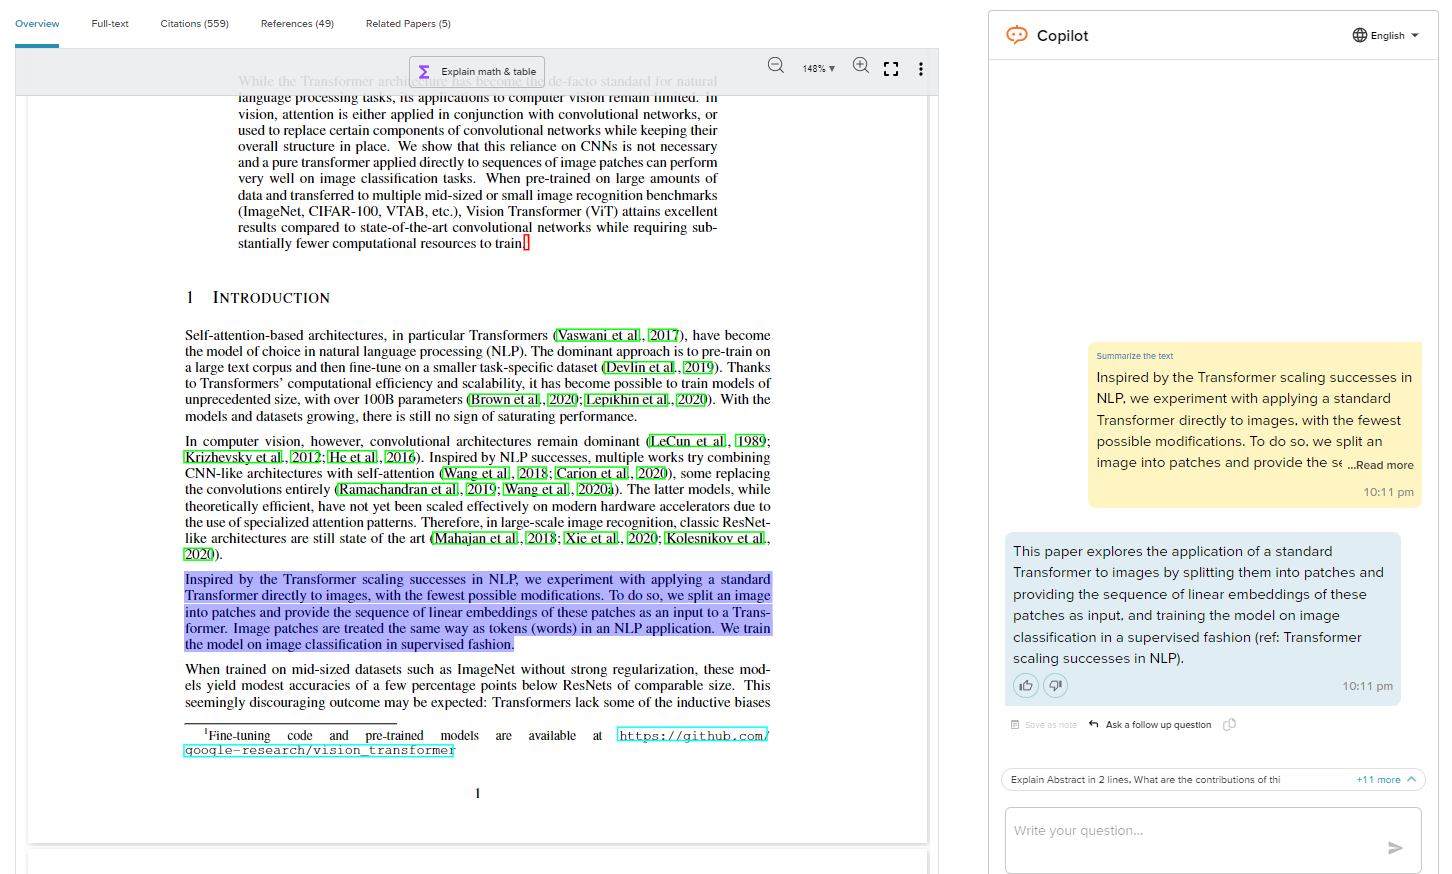
\includegraphics[width=\linewidth]{img/typeset-example.png}
	\caption{Informatie opvragen van een wetenschappelijk artikel met SciSpace}
	\label{img:scispace-example}
\end{figure}

Verder moeten toepassingen een moeilijk woord in een doorlopende tekst kunnen aanpassen. Specifiek kunnen O1, O3, O4 en O5 een annotatie toevoegen aan moeilijke woorden, maar dit gebeurt alleen als er daarvoor geen geschikt synoniem beschikbaar is. Zo illustreert figuur \ref{img:simplish-output} hoe O1 een extra definitie als annotatie kan geven. Hoewel dit het taalniveau niet kan aanpassen, toch laat figuur \ref{img:scholarcy} zien hoe O3 dit probeert in te schatten met een \textit{rewordifying level}. Bovendien kunnen O4 en O5 de doelgroep aanpassen afhankelijk van de \textit{prompts}. Andere uitgeteste tools tonen niet hoe zij de doelgroepinschatting maken. Geen tool laat gebruikers toe om een vooraf opgestelde woordenlijst met moeilijke woorden mee te geven waarop de tool zich kan baseren.

\begin{figure}[H]
	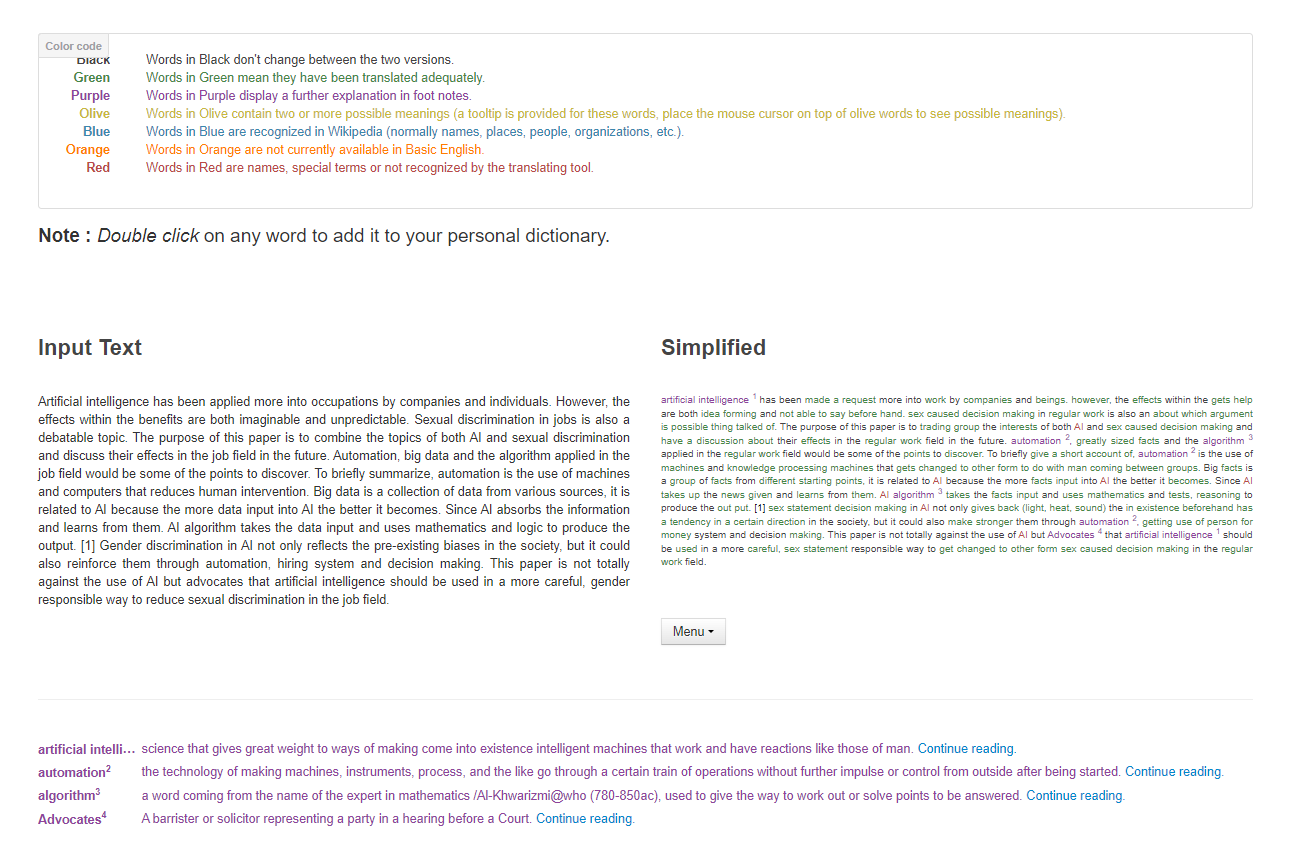
\includegraphics[width=\linewidth]{img/simplish-output.png}
	\caption{Schermafbeelding van de tekstanalyse bij Simplish na een tekstvereenvoudiging.}
	\label{img:simplish-output}
\end{figure}

Daarnaast kunnen toepassingen ook handmatig een woordenlijst maken. Zo kunnen E1, E2, E3 en O1 een woorden- of synoniemenlijst opstellen. Bij deze toepassingen selecteren gebruikers handmatig moeilijke woorden. Die moet de toepassing vereenvoudigen of een definitie ervan ophalen. Uitzonderlijk O1 geeft de woordsoort mee. Verder kunnen gebruikers niet bepalen uit welke bron de definitie moet komen, bijvoorbeeld een online woordenboek. Enkel E1 laat dit toe.

\medspace

Verder kunnen E1, E2 en E3 geen syntactische vereenvoudiging toepassen op de oorspronkelijke tekst. Overige uitgeteste tools kunnen zinnen inkorten door deze te splitsen. Geen van de uitgeteste tools kunnen de geselecteerde tekst automatisch naar een actieve vorm schrijven. In tegenstelling tot O4 en O5 die dit wel kunnen doen, maar enkel als de tool een onderwerp in de prompt meekrijgt. 

\medspace

Tot slot slagen O2, O4 en O5 erin om de tekst te herschrijven als opsomming. Zo doet O2 dit automatisch, vergeleken met O4 en O5 die deze vraag expliciet in hun prompt moeten krijgen. De andere uitgeteste tools kunnen dit niet automatisch doen. 

\subsubsection{Should-haves}

Allereerst tonen O1 en O3 automatisch leesgraadmetrieken nadat die een vereenvoudiging of samenvatting maken van de oorspronkelijke tekst. Zo tonen figuren \ref{img:simplish-output} en \ref{img:scholarcy} een voorbeeld van deze analyse. Deze analyse toont het aantal zinnen en complexe/lange woorden voor zowel het oorspronkelijk als het vereenvoudigde artikel. Andere uitgeteste tools tonen dit niet.

\begin{figure}[H]
	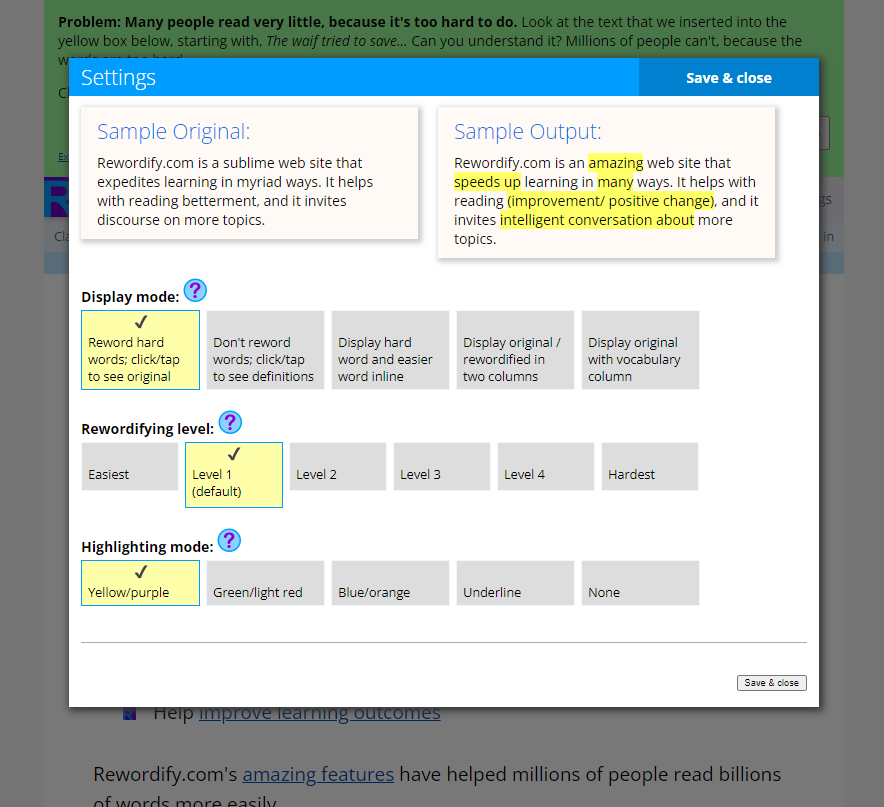
\includegraphics[width=\linewidth]{img/scholarcy-attempt.png}
	\caption{Tekstanalyse met \textit{Rewordify}.}
	\label{img:scholarcy}
\end{figure}

Verder kan het onderzoek niet afleiden of de uitgeteste tools een OCR-techniek gebruiken. Wel gebruikt O2 een andere inleestechniek dan de andere tools. Zo kan het de twee gebruikte wetenschappelijke artikelen inlezen met een identieke lay-out als het oorspronkelijk artikel. Daarna markeert de gebruiker enkel aanpassingen in het artikel, terwijl alle uitvoer van het taalmodel rechts in beeld komt. Echter, de gebruiker kan deze aanpassing niet afleiden uit de oorspronkelijke tekst, in tegenstelling tot O1 en O3. Die tonen wel de verschillen tussen het oorspronkelijk en het vereenvoudigd artikel aan de eindgebruiker.

\subsubsection{Could-haves}

Verschillende geteste tools maken gebruik van gebruikerfeedbacktechnieken in de vorm van \textit{pop-ups}, zoals bij een aanpassing van de tekst. O4 en O5 vormen hierop een uitzondering, omdat zij deze technieken niet bevatten. Uitzonderlijk O4 en O5 kunnen tekst omzetten naar een tabelformaat, maar dit gebeurt alleen na een expliciete prompt. Ze hebben de mogelijkheid om tekst te interpreteren en deze in een tabel te gieten. Zo maken ze gebruik van een 2 op 2 tabel, maar de gebruiker kan het aantal kolommen en rijen instellen via de prompt.

\medspace

Geen van de geteste tools kan automatisch moeilijke woorden of vakterminologie extraheren uit een tekst, behalve O4 en O5, die dit wel kunnen met behulp van een expliciete prompt.

\medspace

Wat betreft samenvattingen kunnen O1, O2, O3, O4 en O5 zowel extraherende als abstraherende samenvattingen maken van de oorspronkelijke tekst. E1, E2 en E3 kunnen alleen een extraherende samenvatting maken, maar dit gebeurt pas na een handmatige selectie van de zinnen.

\medspace

Alleen O4 en O5 hebben de mogelijkheid om een gegeven tekst te herschrijven. Dezelfde prompt kan leiden tot een ontelbaar aantal resultaten. Alle andere toepassingen slagen hier niet in en alle versies van een herschreven artikel leiden tot hetzelfde resultaat. Tot slot kunnen enkel O1, O2, O4 en O5 wel onregelmatige werkwoorden corrigeren.

\subsubsection{Wont-haves}

Op het vlak van toegankelijkheid beschikken O4 en O5 over een mobiele versie. Daarnaast kan een gebruiker O1, O2 en O3 wel via een mobiel apparaat bekijken, maar deze lenen geen speciale interface toe. Vervolgens bieden E1, E2 en E3 geen mobiele versie aan. 

\medspace

Daarnaast beschikken enkel E1, E2 en E3 over luistersoftware. Hoewel browsers over ingebouwde luistertools beschikken, toch bieden de andere tools geen personaliseerbare \textit{text-to-speech} techniek aan. Tot slot beschikken de geteste toepassingen over geen integratie met andere spelcheckers. Wel werkt de browserextensie van \textit{Grammarly} bij zowel O1, O2, O3, O4 en O5. 

\section{Geschikte taalmodel voor gepersonaliseerde tekstvereenvoudiging met ATS}

De vergelijkende studie evalueert de uitvoer van de uitgeteste taallmodellen, opgesomd in \ref{table:vergelijkende-studie-taalmodellen}, met een machinale en een menselijke beoordeling. Zo achterhaalt deze onderzoeksmethode welk taalmodel of LLM beter aansluit bij het aanbieden van gepersonaliseerde ATS voor scholieren met dyslexie in de derde graad van het middelbaar onderwijs. 

\subsubsection{Machinale beoordeling van de vereenvoudigde teksten}

Tabel \ref{table:resultaten-aantal-zinnen} geeft het aantal zinnen per (vereenvoudigd) artikel. De MTS-referentieteksten bevatten minder zinnen dan het oorspronkelijk artikel. Het aantal zinnen na ATS met T1, T2 en T3 is gehalveerd tot minder dan een kwart van oorspronkelijke hoeveelheid zinnen. Enkel T4P2 genereert meer zinnen dan de oorspronkelijke versie van A1 na ATS. T4P2 genereert bij zowel A1 als A2 meer zinnen vergeleken met de andere geteste taalmodellen. T2 daarentegen genereert bij beide artikelen het minst aantal zinnen. Figuren \ref{img:boxplot-min-max-avg-words-a1} en \ref{img:boxplot-min-max-avg-words-a2} illustreren deze verschillen tussen de taalmodellen.

\begin{table}[h]
	\centering
	\begin{tabular}{ | m{3cm} | m{3cm} | m{3cm} | } 
		\hline
		\textbf{Bron} & \textbf{#Zinnen in A1} & \textbf{#Zinnen in A2} \\
		\hline
		Oorspronkelijk & 78  & 159 \\ 
		\hline
		MTS (door leerkracht) & 43 & 45 \\
		\hline
		MTS (door leerling) & n.v.t. & 50 \\
		\hline
		T1 & 26 & 24 \\
		\hline
		T2 & 11 & 7 \\
		\hline
		T3 & 67 & 130 \\
		\hline
		T4 P1 & 61 & 98 \\
		\hline
		T4 P2 & 89 & 133 \\
		\hline
		T4 P3 & 39 & 55 \\
		\hline
	\end{tabular}
	\caption{Aantal zinnen (gemeten met Spacy sentence embeddings) per tekst.}
	\label{table:resultaten-aantal-zinnen}
\end{table}

\begin{figure}[H]
	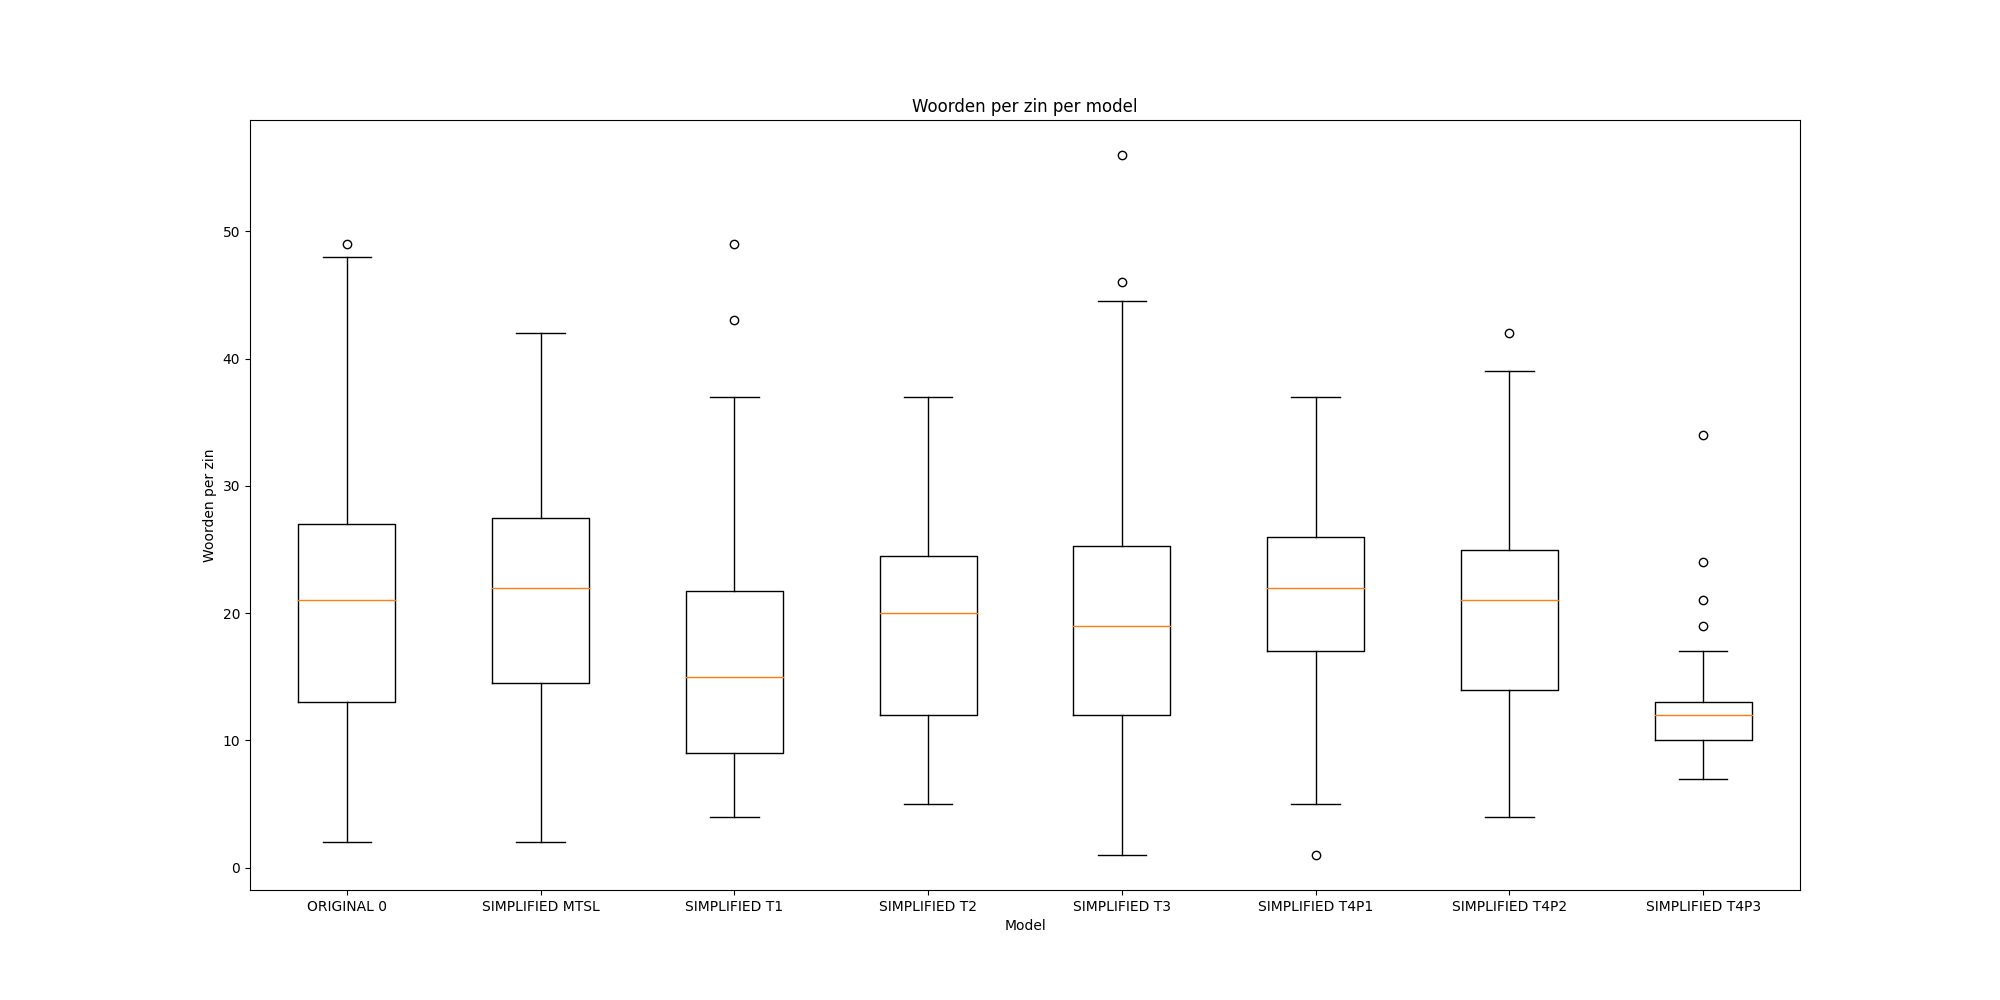
\includegraphics[width=\linewidth]{img/boxplot-avg-a1.png}
	\caption{Overzicht van het minimum, maximum en gemiddeld aantal woorden per zin per model in A1.}
	\label{img:boxplot-min-max-avg-words-a1}
\end{figure}

\begin{figure}[H]
	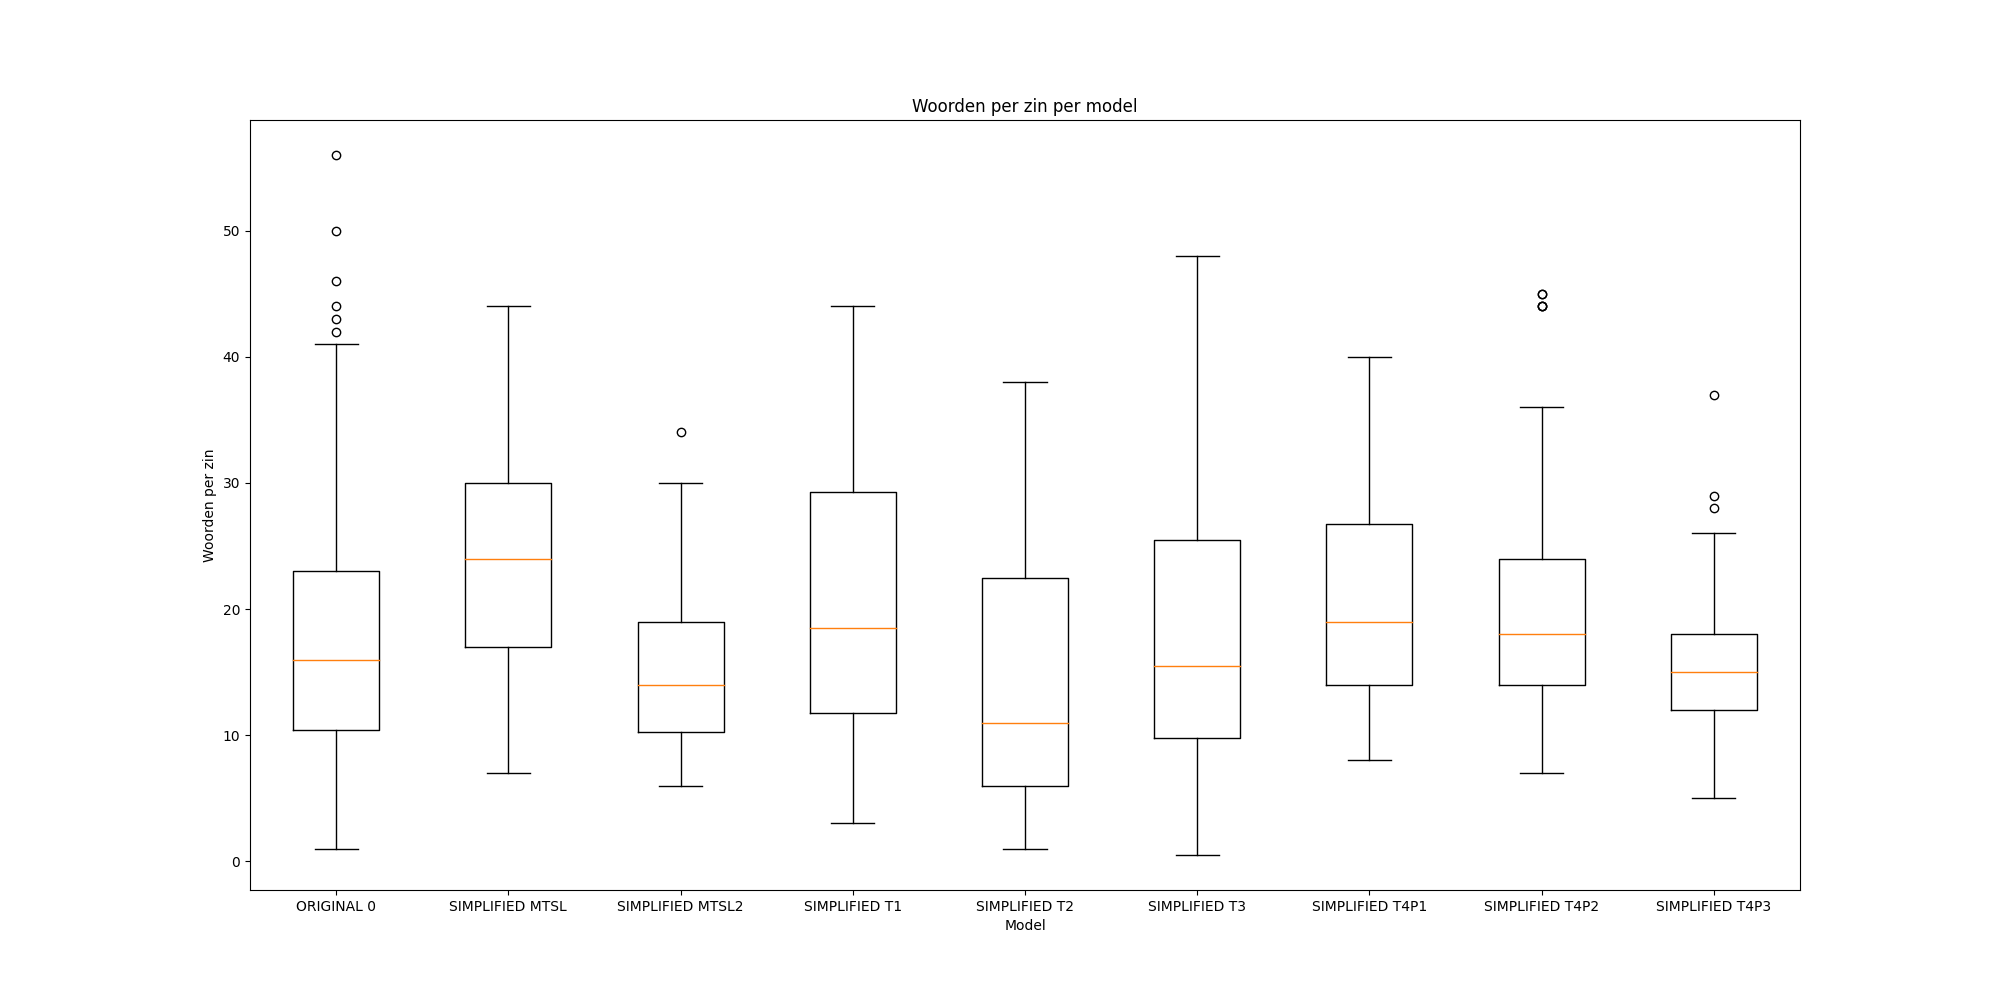
\includegraphics[width=\linewidth]{img/boxplot-avg-a2.png}
	\caption{Overzicht van het minimum, maximum en gemiddeld aantal woorden per zin per model in A2.}
	\label{img:boxplot-min-max-avg-words-a2}
\end{figure}

Verder vergelijkt het onderzoek de verkregen leesbaarheidsscores per zin dat ieder taalmodel kan genereren. Allereerst de FRE-scores die de leesgraad van een zin aanduidt. Alle geteste taalmodellen genereren zinnen waarvan de FRE-scores niet opmerkelijk hoger of lager zijn ten opzichte van het oorspronkelijk artikel. Figuren \ref{img:boxplot-fre-a1} en \ref{img:boxplot-fre-a2} tonen deze verschillen. Gemiddeld bevinden alle versies van het wetenschappelijk artikel zich tussen 20 en 50. Zonder \textit{outliers} beperkt T3 de FRE van alle zinnen tot hoogstens 40. T3, T4P1, T4P2 en T4P3 genereren zinnen met een hogere FRE dan OG en MTSL. 

\begin{figure}[H]
	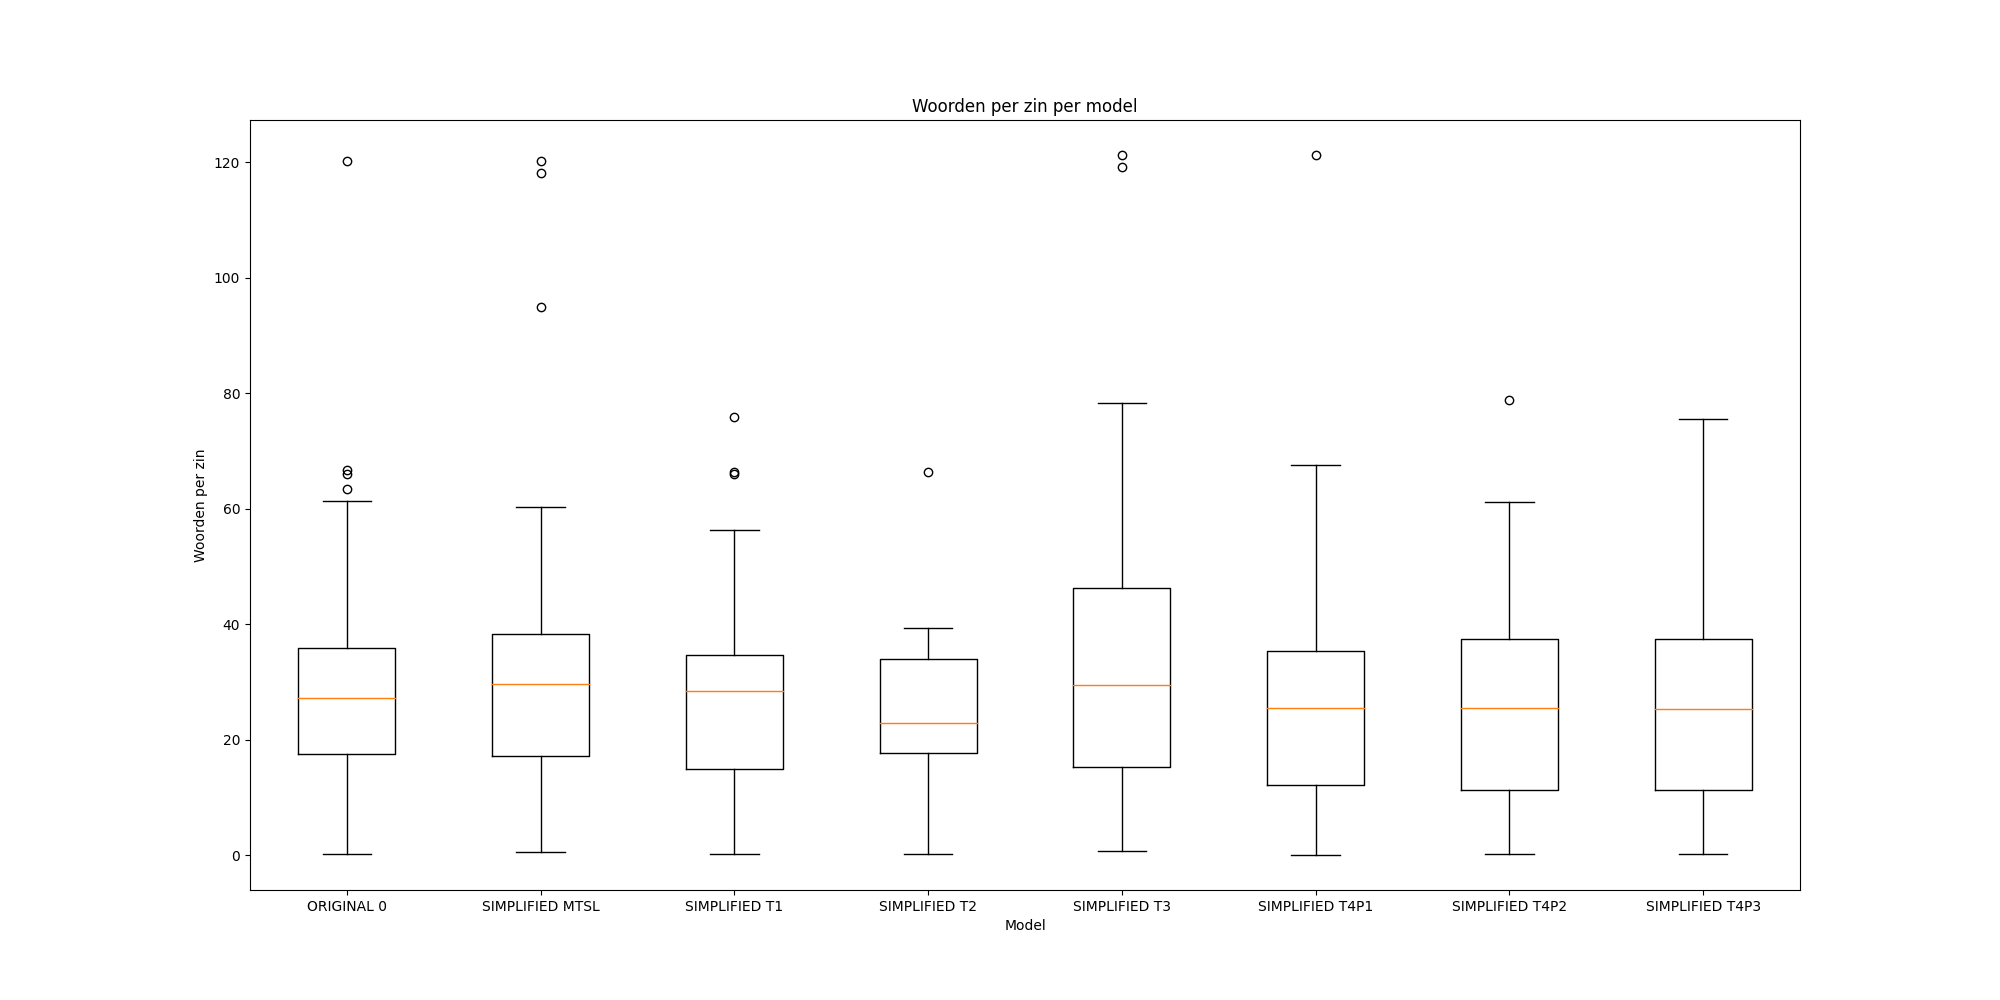
\includegraphics[width=\linewidth]{img/boxplot-fre-a1.png}
	\caption{Boxplot van de FRE-scores voor A1.}
	\label{img:boxplot-fre-a1}
\end{figure}

\begin{figure}[H]
	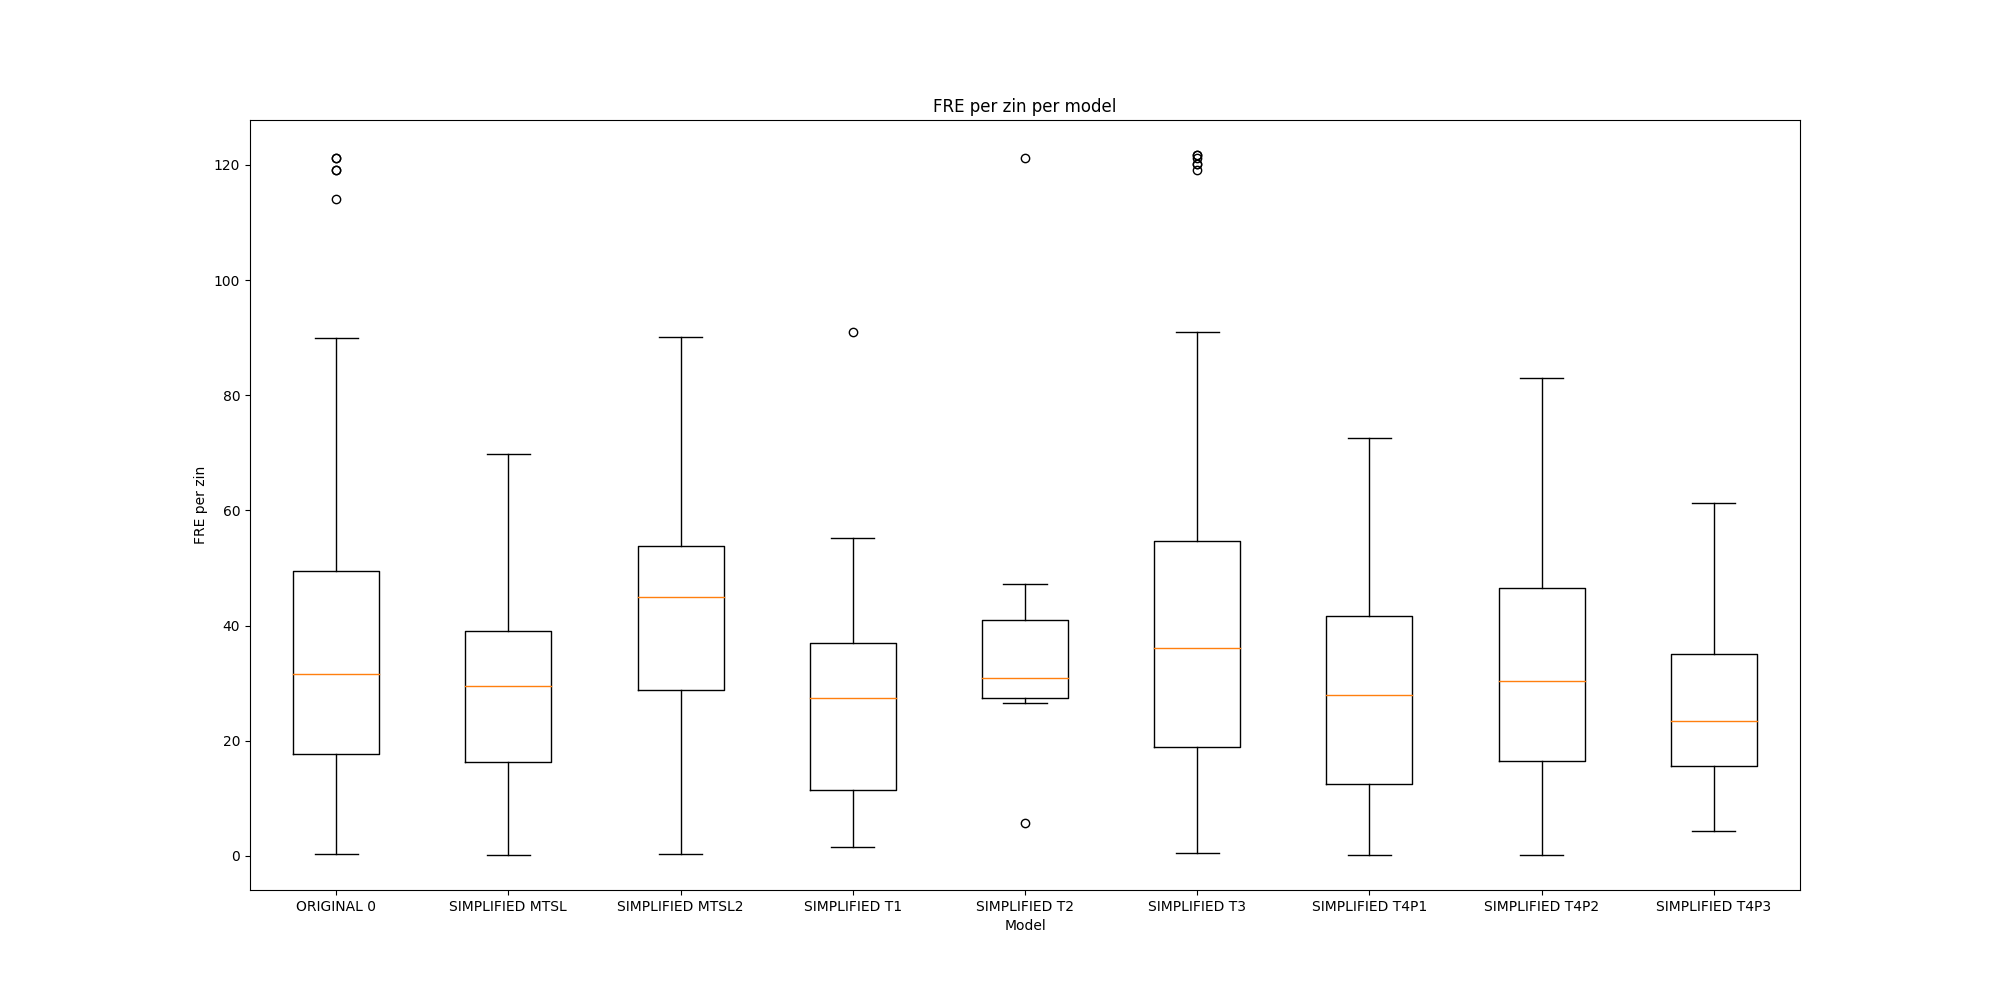
\includegraphics[width=\linewidth]{img/boxplot-fre-a2.png}
	\caption{Boxplot van de FRE-scores voor A2.}
	\label{img:boxplot-fre-a2}
\end{figure}

De FOG-scores van alle geteste taalmodellen en MTS-referentieteksten zijn niet opmerkelijk hoger of lager bij de vereenvoudigde wetenschappelijke artikelen, zoals weergegeven in figuren \ref{img:boxplot-fog-a1} en \ref{img:boxplot-fog-a2}. De zinnen van MTSL2 en T2 scoren gemiddeld lagere FOG-scores dan OG. Daarnaast scoort T2 een lager gemiddelde dan andere taalmodellen. Dit gemiddelde ligt tussen 10 en 12. Tot slot scoren MTSL en andere taalmodellen gemiddeld hoger dan OG. Tot slot genereren de taalmodellen geen zinnen met een hogere FOG-score dan OG.

\begin{figure}[H]
	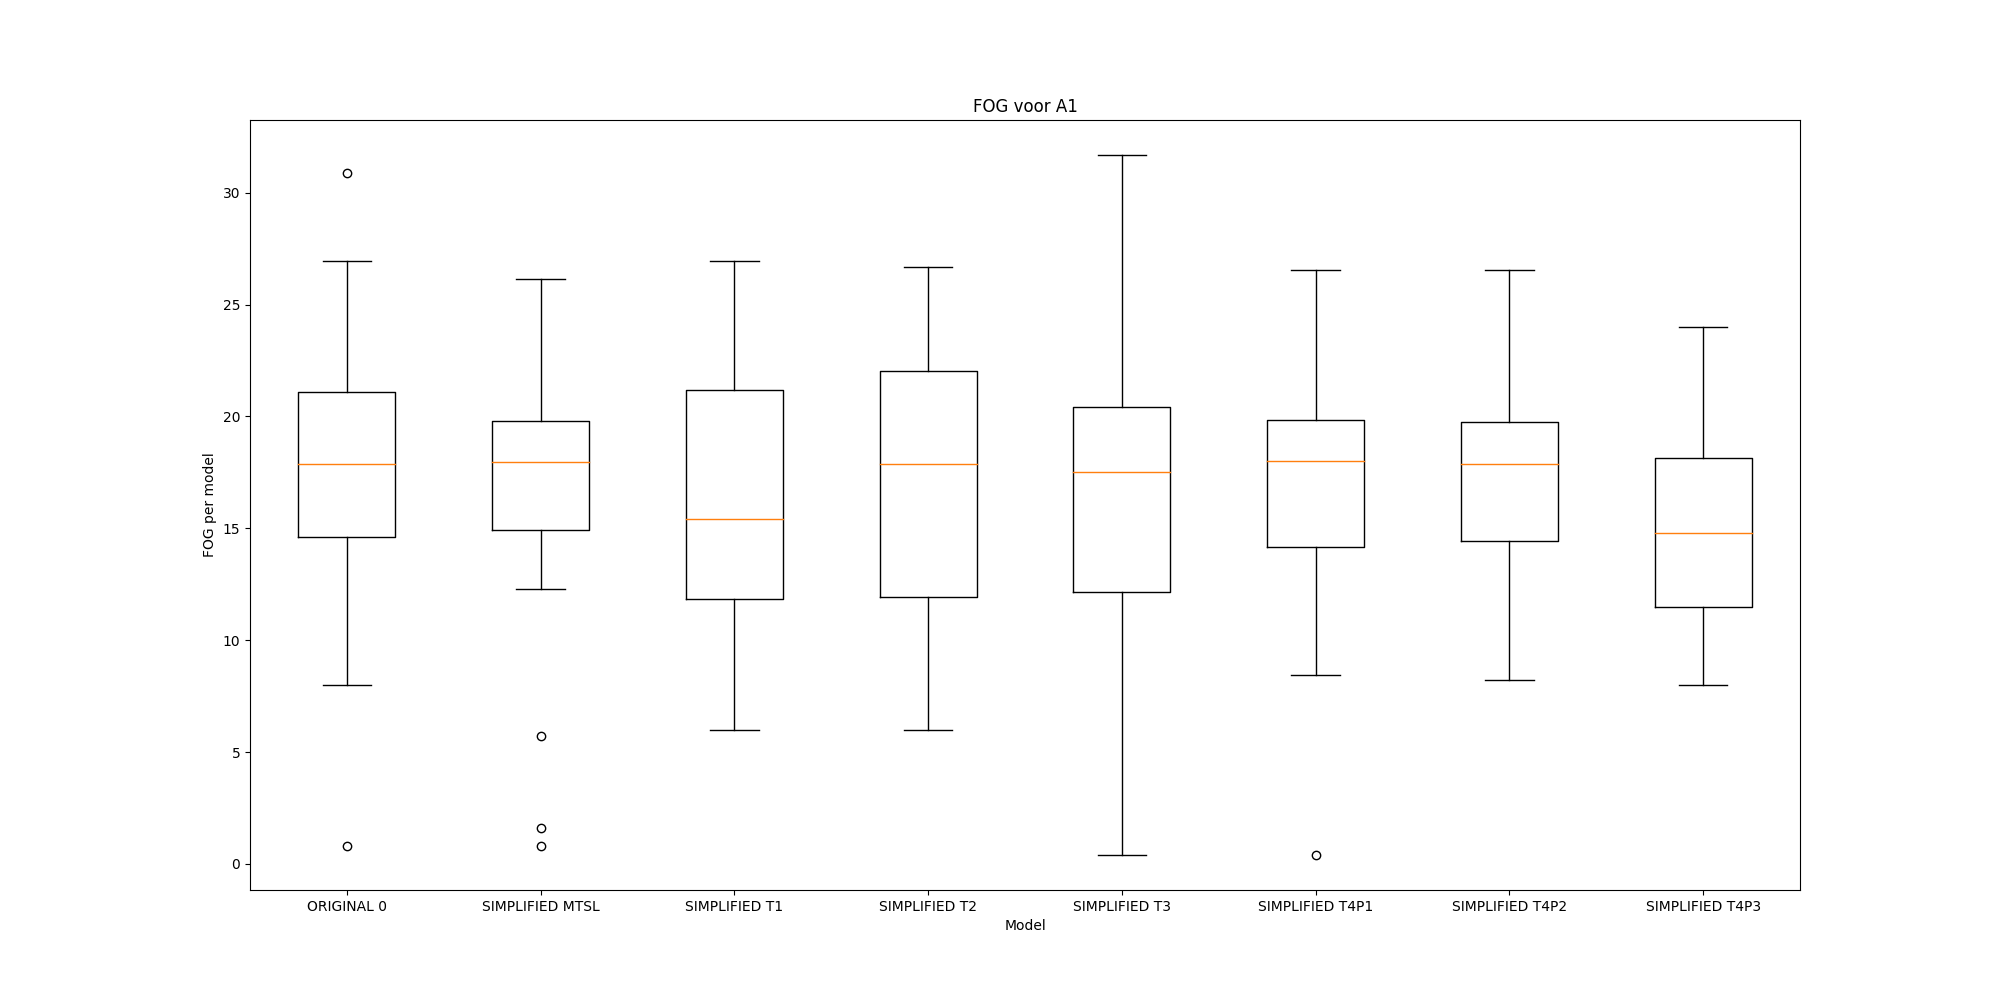
\includegraphics[width=\linewidth]{img/boxplot-fog-a1.png}
	\caption{Boxplot van de FOG-scores voor A1.}
	\label{img:boxplot-fog-a1}
\end{figure}

\begin{figure}[H]
	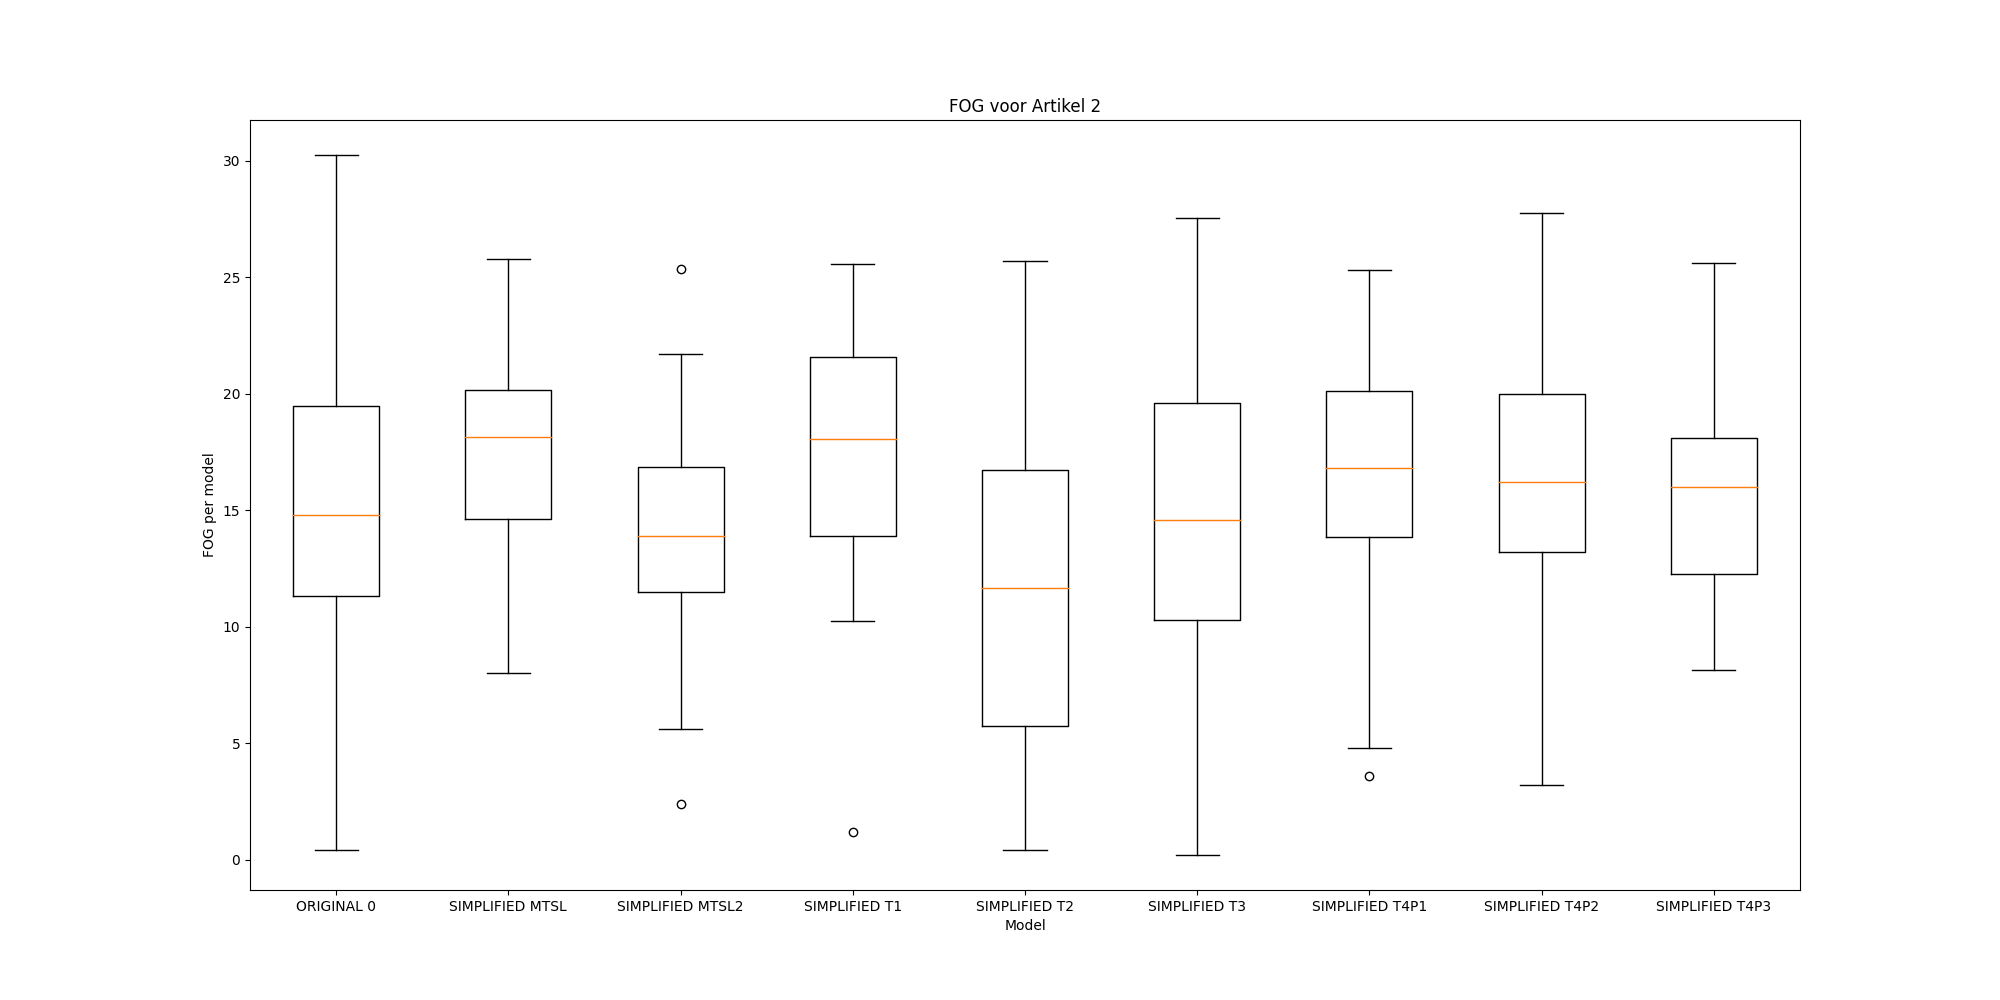
\includegraphics[width=\linewidth]{img/boxplot-fog-a2.png}
	\caption{Boxplot van de FOG-scores voor A2.}
	\label{img:boxplot-fog-a2}
\end{figure}

T1, T2 en T3 genereren meer complexe woorden vergeleken met T4, MTSL en OG. Bij A1 genereert T4P3 opmerkelijk minder complexe woorden per zin dan de andere taalmodellen. Bij A2 is er geen opmerkelijk verschil tussen de taalmodellen. Vervolgens visualiseren figuren \ref{img:violinplot-long-a1} en \ref{img:violinplot-long-a2} het aantal lange woorden per zin. Het systeem betrekt een woord met minstens vier lettergrepen als een lang woord. MTSL, T2, T4P1, T4P2 en T4P3 genereren minder lange woorden per zin dan OG.

\begin{figure}[H]
	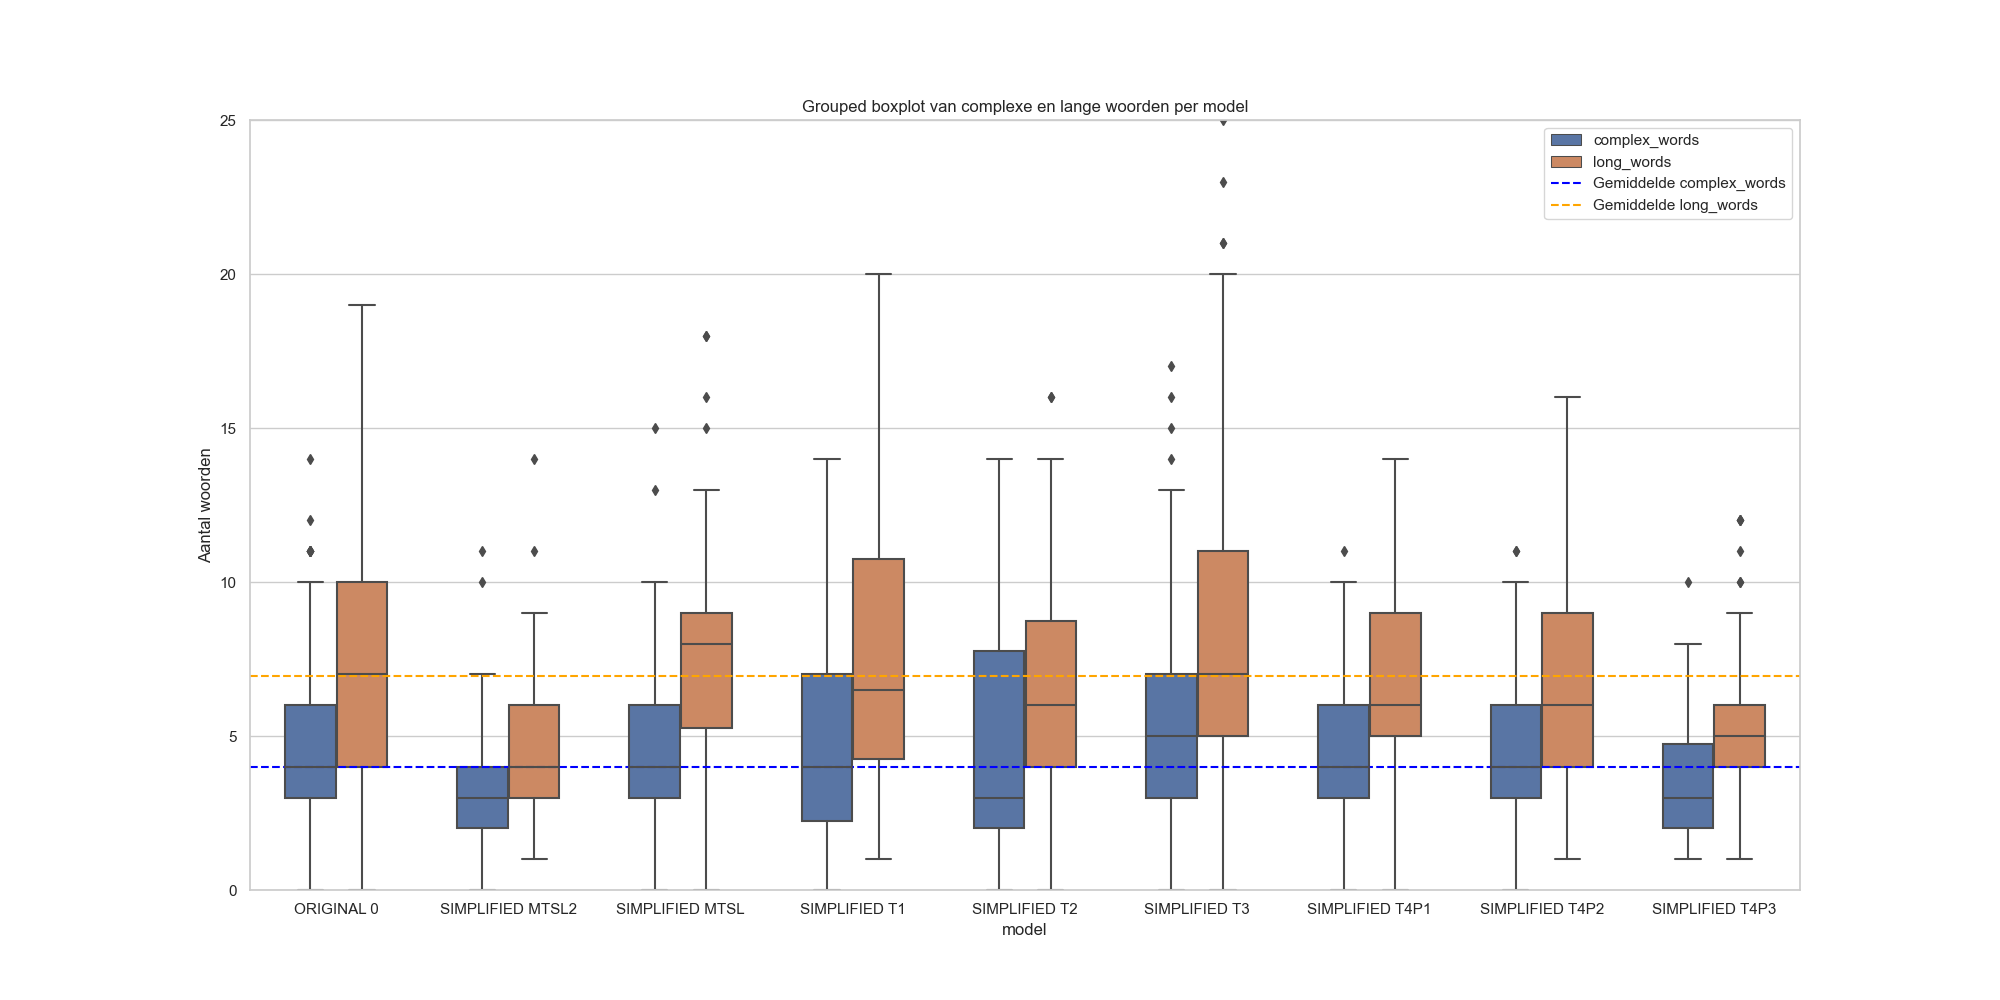
\includegraphics[width=\linewidth]{img/boxplot-poster.png}
	\caption{Een boxplot van het aantal lange en complexe woorden per zin, gegroepeerd op model voor A1.}
	\label{img:long-complex-words}
\end{figure}


Vervolgens tonen figuren \ref{img:histplot-aux-a1} en \ref{img:histplot-aux-a2} het aantal hulpwerkwoorden in de tekst. Deze figuren zijn geen absolute percentages en houden geen rekening met het aantal zinnen. Ten slotte tonen \ref{img:histplot-aux-a1} en \ref{img:histplot-aux-a2} het aantal vervoegingen van het werkwoord 'zijn' aan. 

\begin{figure}[H]
	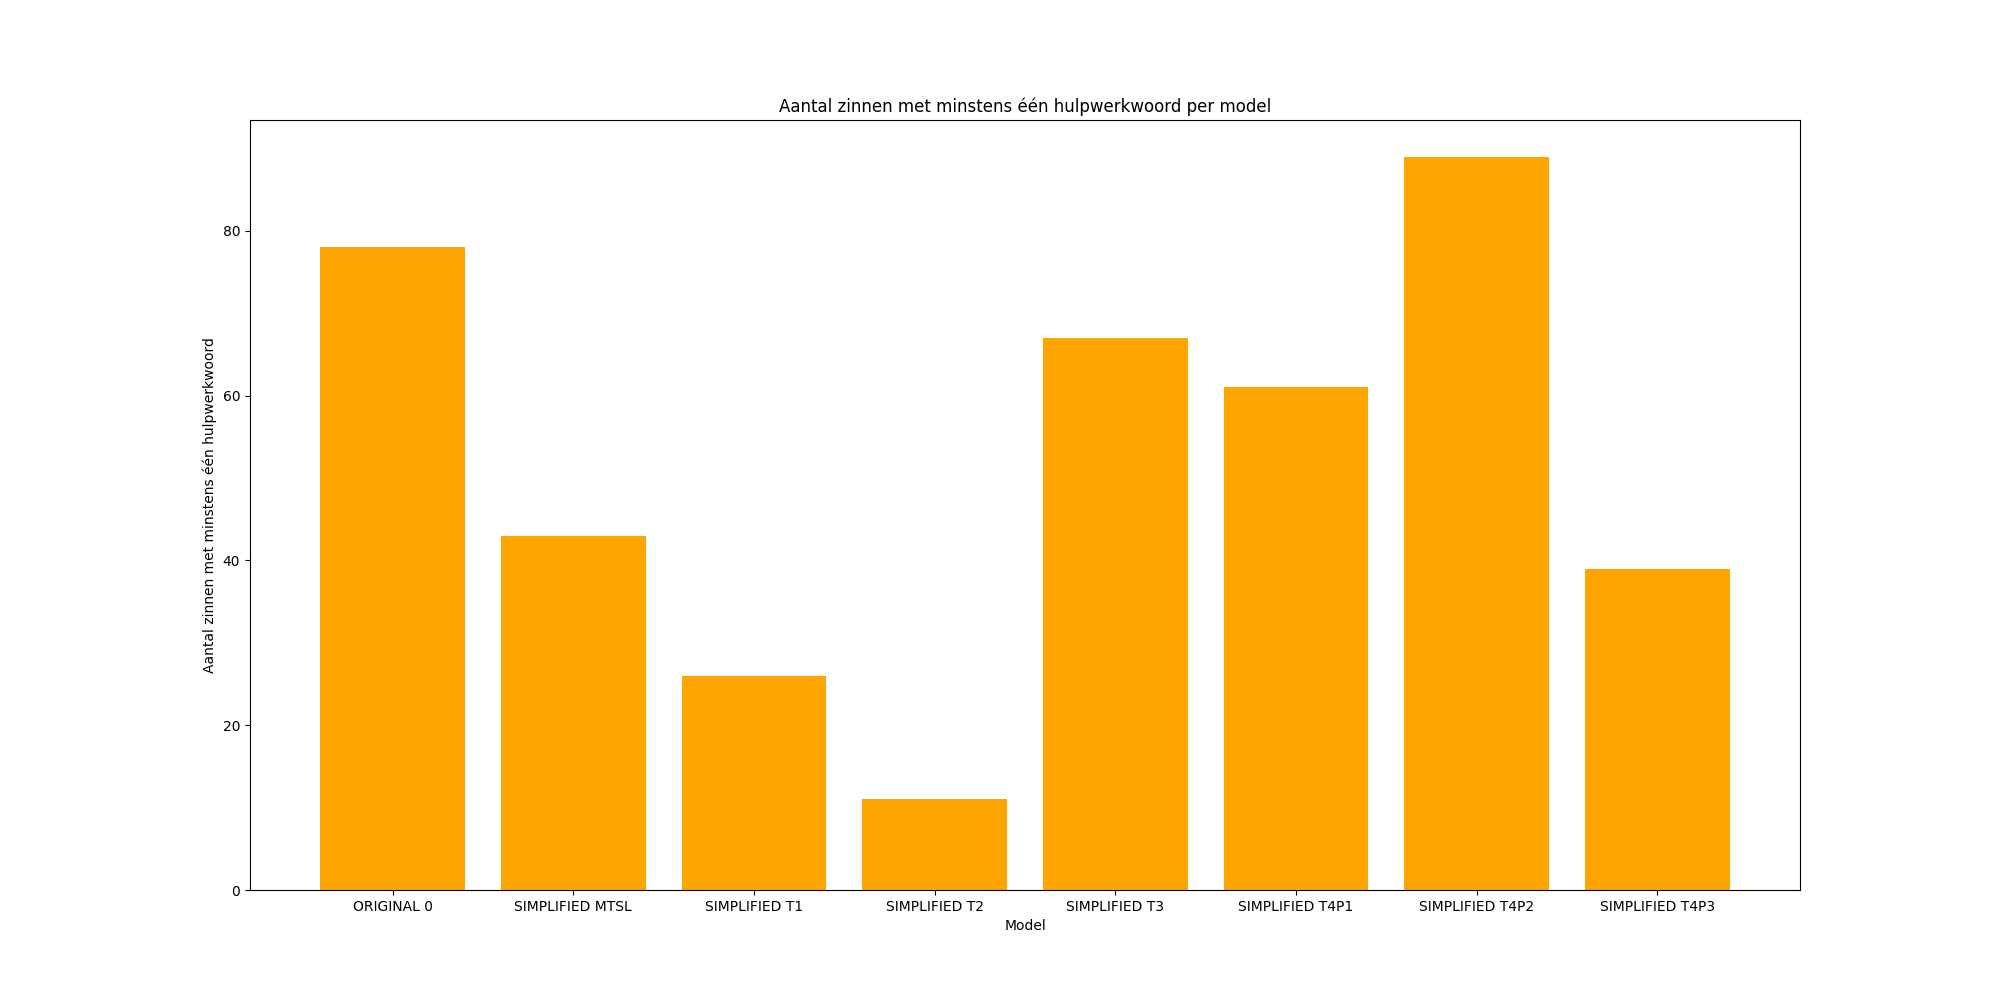
\includegraphics[width=\linewidth]{img/boxplot-aux-a1.png}
	\caption{Een staafdiagram van het aantal gebruikte hulpwerkwoorden in de tekst, gegroepeerd op model voor A1.}
	\label{img:histplot-aux-a1}
\end{figure}

\begin{figure}[H]
	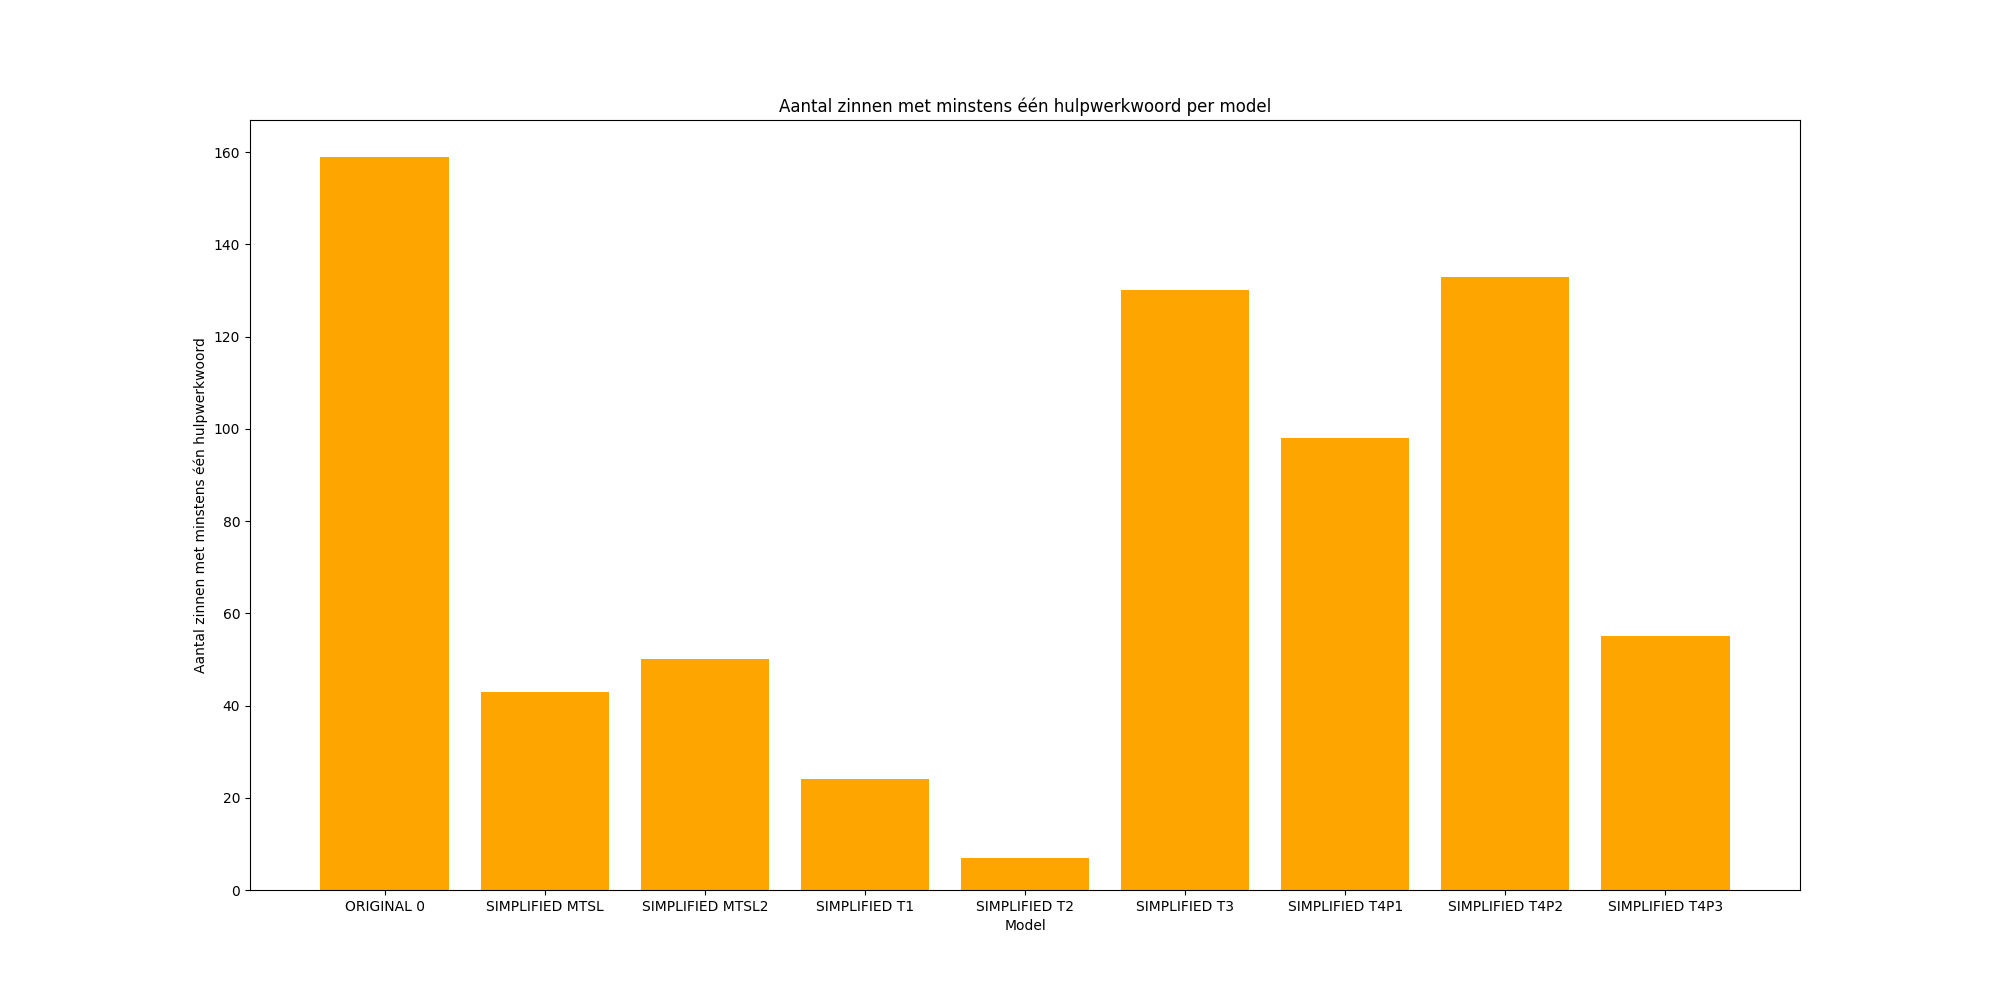
\includegraphics[width=\linewidth]{img/boxplot-aux-a2.png}
	\caption{Een staafdiagram van het aantal gebruikte hulpwerkwoorden in de tekst, gegroepeerd op model voor A2.}
	\label{img:histplot-aux-a2}
\end{figure}

\begin{figure}[H]
	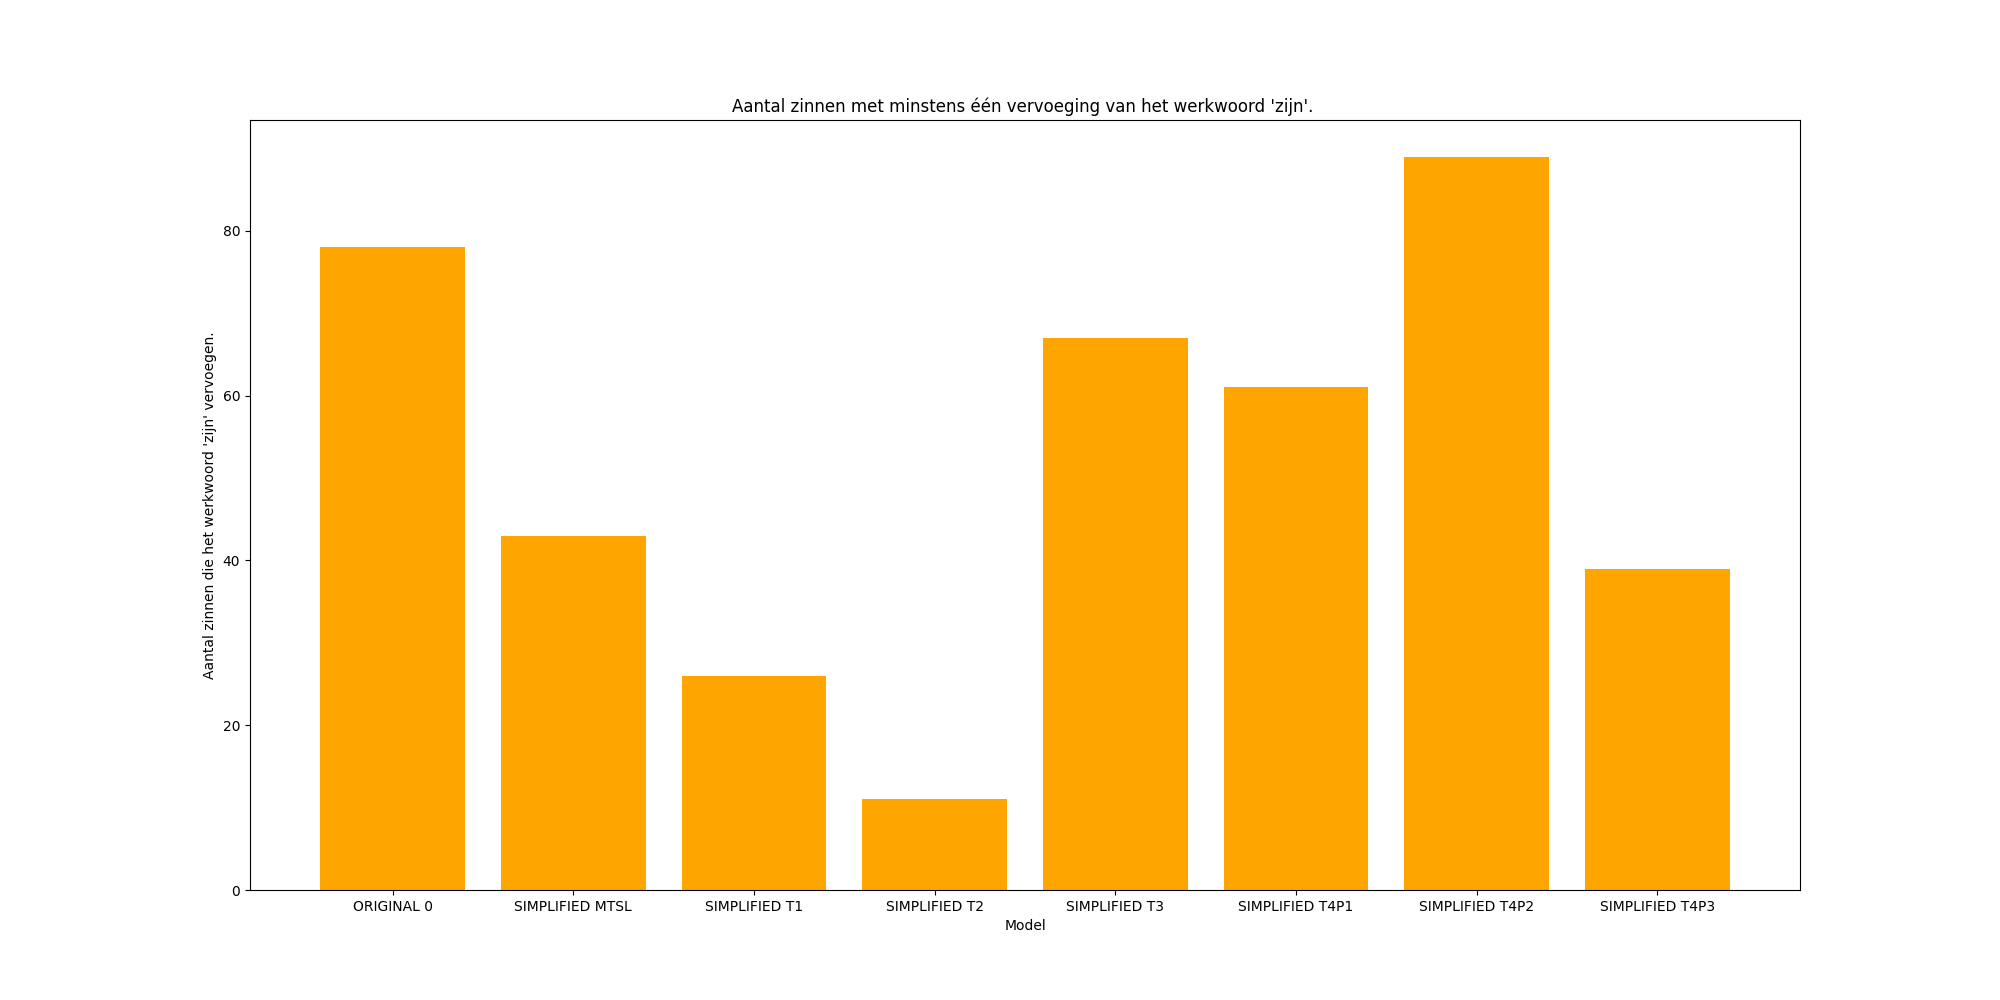
\includegraphics[width=\linewidth]{img/boxplot-tobe-a1.png}
	\caption{Het aantal vervoegingen van het werkwoord 'zijn', gegroepeerd op model voor A1.}
	\label{img:histplot-tobe-a1}
\end{figure}

\begin{figure}[H]
	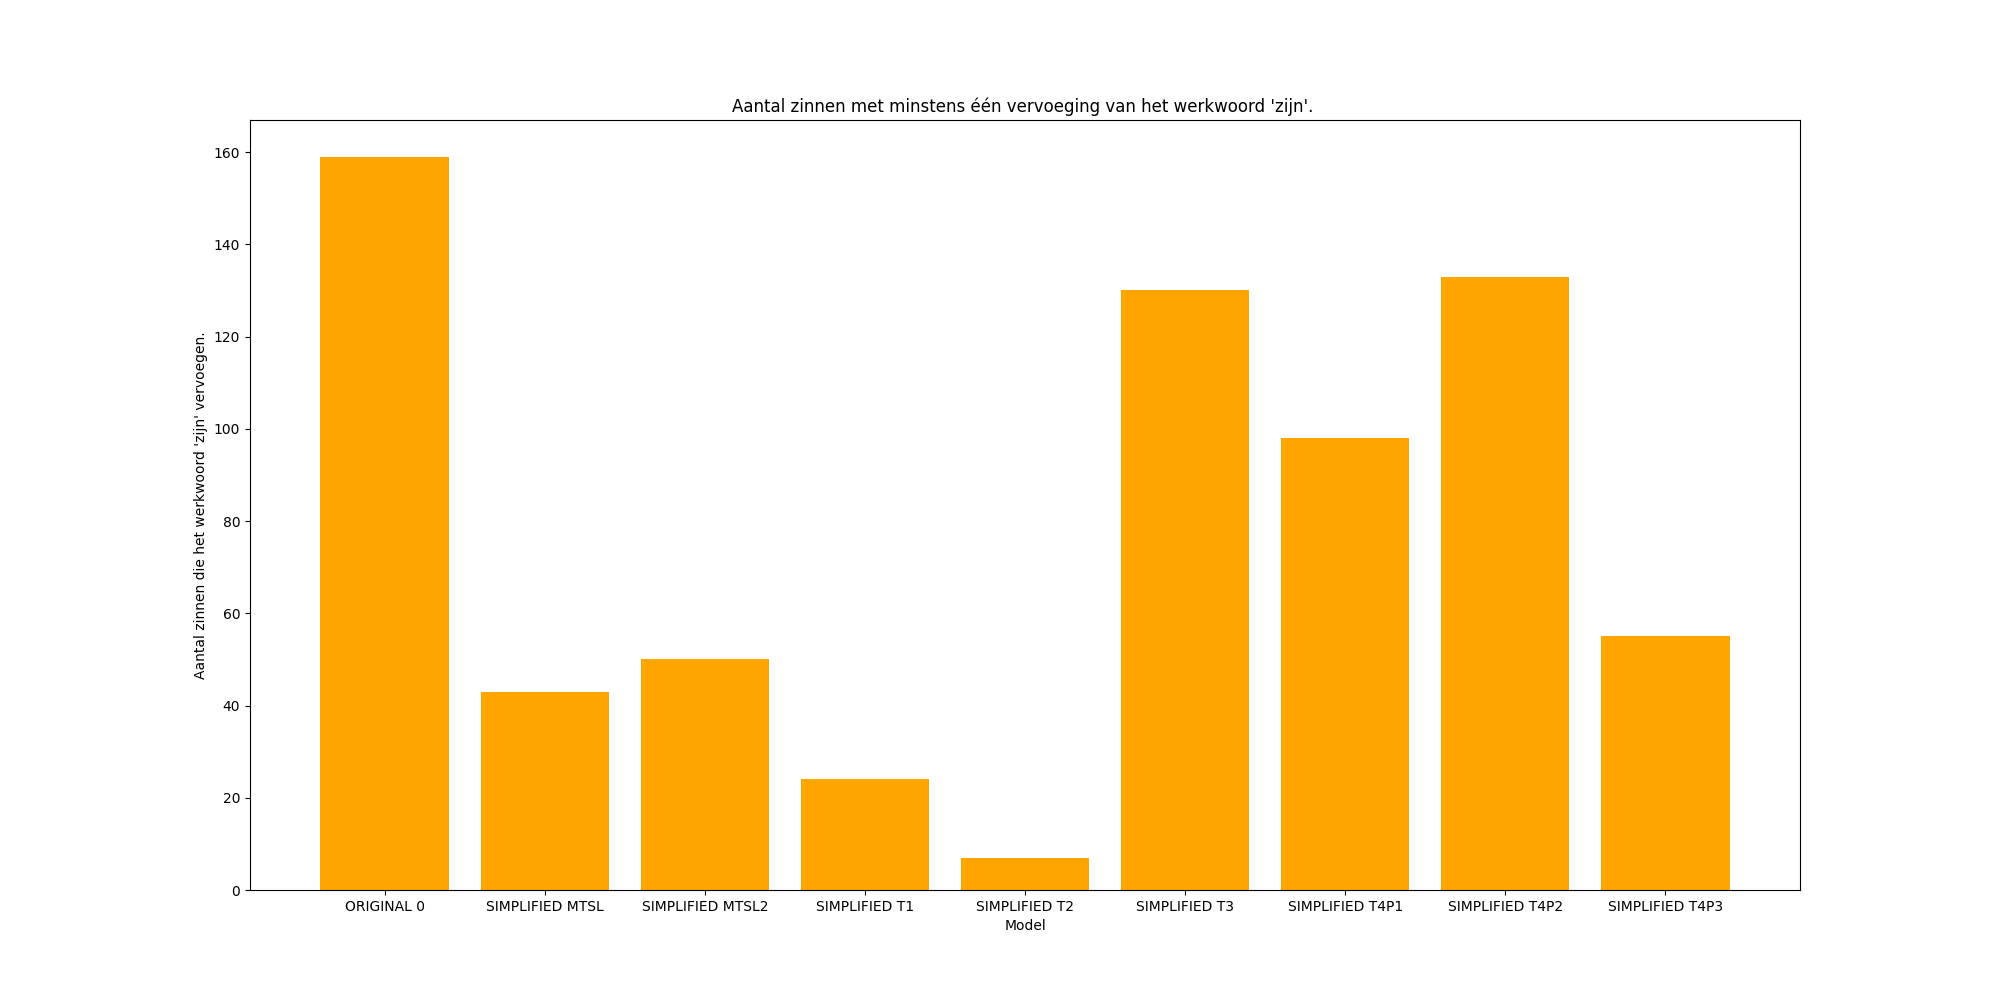
\includegraphics[width=\linewidth]{img/boxplot-tobe-a2.png}
	\caption{Het aantal vervoegingen van het werkwoord 'zijn', gegroepeerd op model voor A2.}
	\label{img:histplot-tobe-a2}
\end{figure}

\subsubsection{Menselijke beoordeling van de referentieteksten.}

In het volgende deel bespreekt het onderzoek de menselijke beoordeling van de resultaten. Allereerst kunnen T4P1 en T4P2 Engelstalige vaktermen vertalen naar het Nederlands. Zo blijft de afkorting voor 'DPKIA' intact, maar vertaalt T4P1 hetzelfde woord naar het Nederlands.  T1, T2, T3 en T4P3 houden hier echter geen rekening mee en behouden de oorspronkelijke versie van de tekst. De auteurs schrijven alle afkortingen voluit, zoals beschreven in de richtlijnen. Zo toont figuur \ref{img:vergelijking-taalmodellen} deze verschillen.

\begin{figure}[H]
	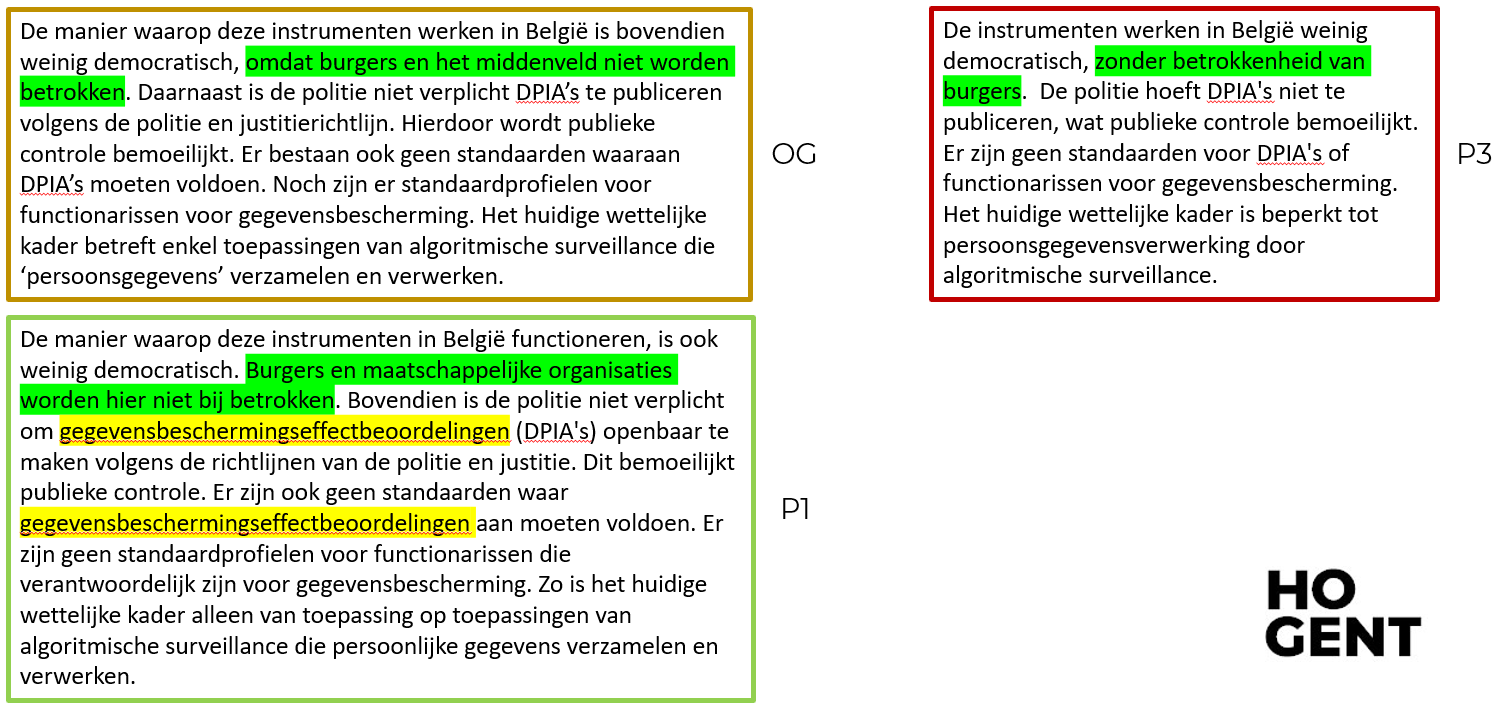
\includegraphics[width=\linewidth]{img/vergelijking.png}
	\caption{De verschillen tussen de oorspronkelijke tekst, T4P1 en T4P3 bij één uitgekozen paragraaf.}
	\label{img:vergelijking-taalmodellen}
\end{figure}

Alle taalmodellen kunnen LS toepassen. De handmatig vereenvoudigde referentieteksten bevatten zinnen die vakjargon gebruiken op het niveau van 15 tot 18 jarige studenten. T4P1 kan uitleg tussen ronde haakjes schrijven, wanneer het geen eenvoudiger synoniem kan vinden. T4P1, T1, T2 en T3 passen woorden aan, maar schrijven geen extra uitleg. T4P3 past deze techniek minder toe dan de vooraf vermelde taalmodellen. T4P3 verkort lange zinnen door deze op te splitsen. T1, T2 en T3 behalen een gelijke zinslengte als dat van de oorspronkelijke zin. T4P1 en T4P2 kunnen langere zinnen genereren, maar smelten geen twee zinnen met elkaar samen. 

\medspace

Geen taalmodel wijkt af van de hoofdgedachte van het oorspronkelijke wetenschappelijk artikel. Hoewel T1, T2 en T3 deels afgebroken zinnen kan genereren, bevatten deze zinnen de hoofdgedachte. T2 bevat minder dan 10\% van het oorspronkelijk artikel en ontbreekt daarbij bijzaken die nodig zijn om alle vragen in \ref{ch:referentietekst} te kunnen begrijpen en te beantwoorden. Tenslotte verwerken T1, T2 en T3 de APA- en California bronvermeldingen niet in de vereenvoudigde teksten. Hoewel T4 deze wel verwerkt, bevat de tekst na een vereenvoudiging deze bronvermeldingen niet meer.

\medspace

Ter conclusie van de resultaten scoren de drie prompts van T4 beter bij de menselijke beoordeling van de resultaten. Het taalmodel en de verwante drie prompts genereren coherente teksten met een verlaagde lexicale complexiteit. Echter houden de geteste taalmodellen weinig tot geen rekening met afkortingen of bronvermeldingen.

\section{Pentimentor vergelijken met \textit{top-of-the-line} tools.}

Gebruikers kunnen vanuit de homepagina drie schermen kiezen: het lerarencomponent, het scholierencomponent en een instellingenpagina. Op de instellingenpagina kunnen eindgebruikers hun persoonlijke opmaak toevoegen. Zo toont figuur \ref{img:website-instellingen} alle mogelijke opmaakopties die Pentimentor aanreikt.

\begin{center}
	\begin{figure}[H]
		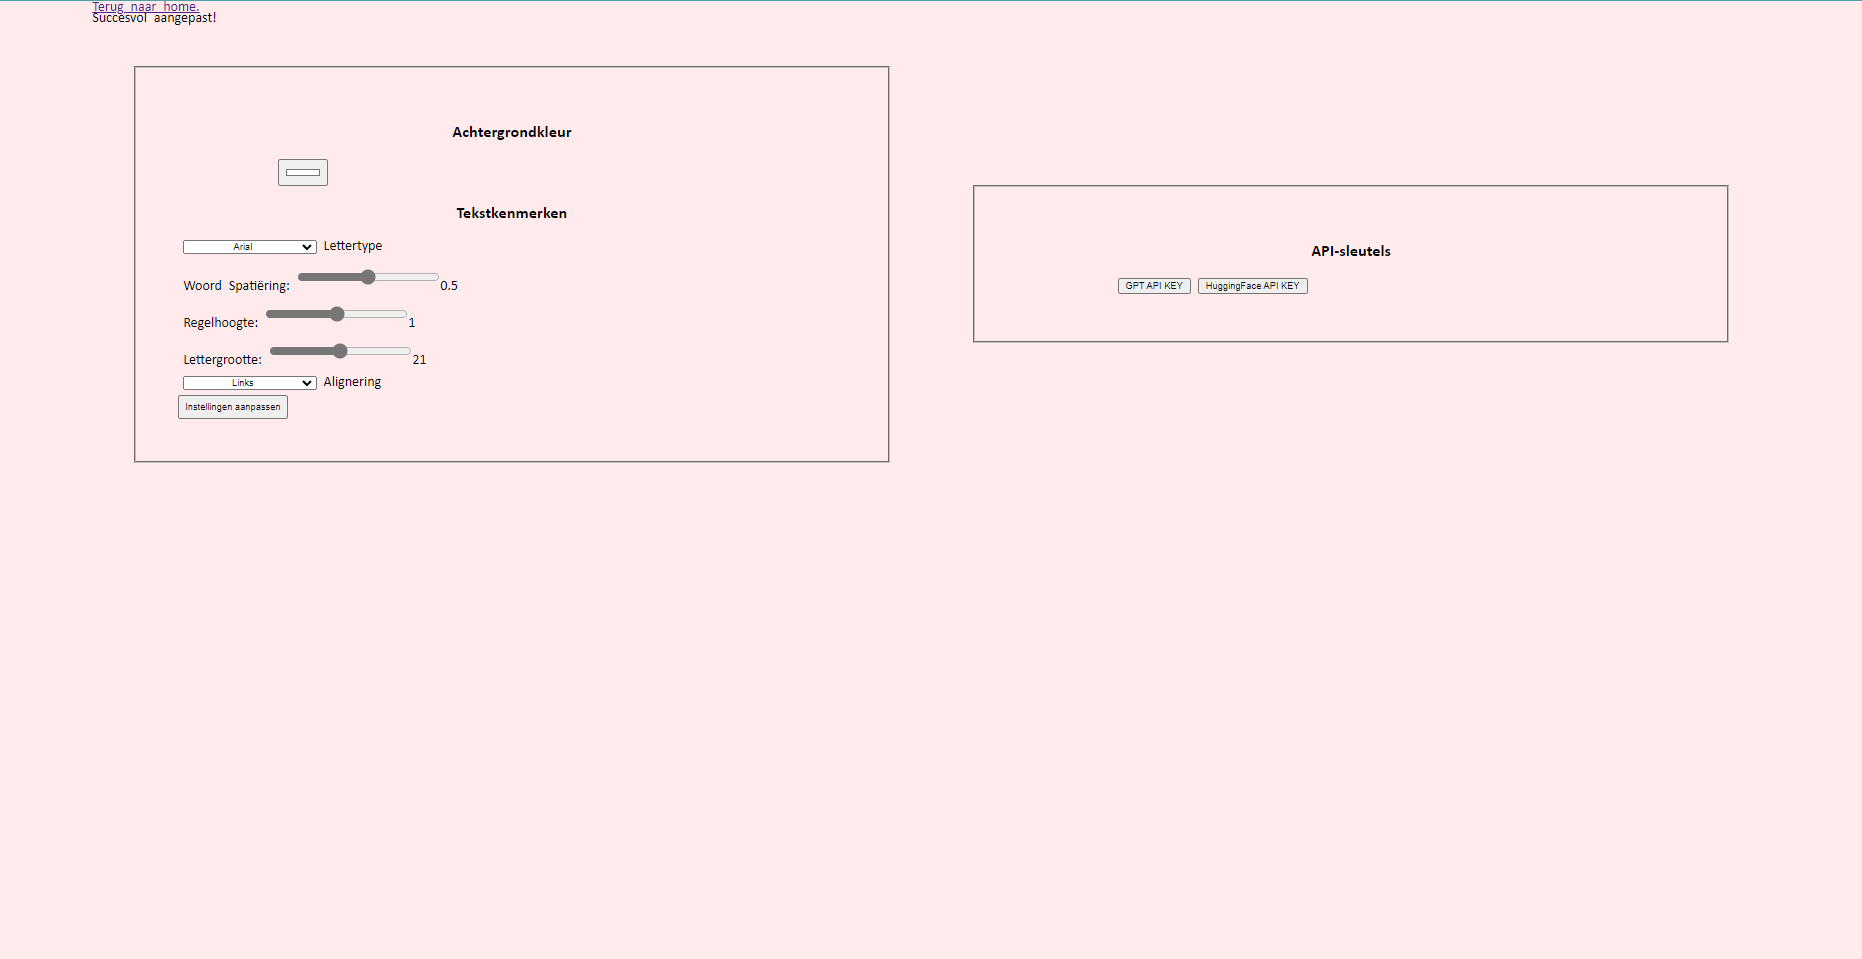
\includegraphics[width=\linewidth]{img/website-instellingen.png}
		\caption{Voorbeeldweergave van de instellingenpagina.}
		\label{img:website-instellingen}
	\end{figure}
\end{center}

Bovendien stelt Pentimentor gebruikers in staat om op basis van gekregen parameters automatisch personaliseerbare docx-documenten te genereren. Zo toont figuur \ref{img:proto-pos-tagging-scholieren} een voorbeeldweergave van deze functionaliteit.

\begin{center}
	\begin{figure}[H]
		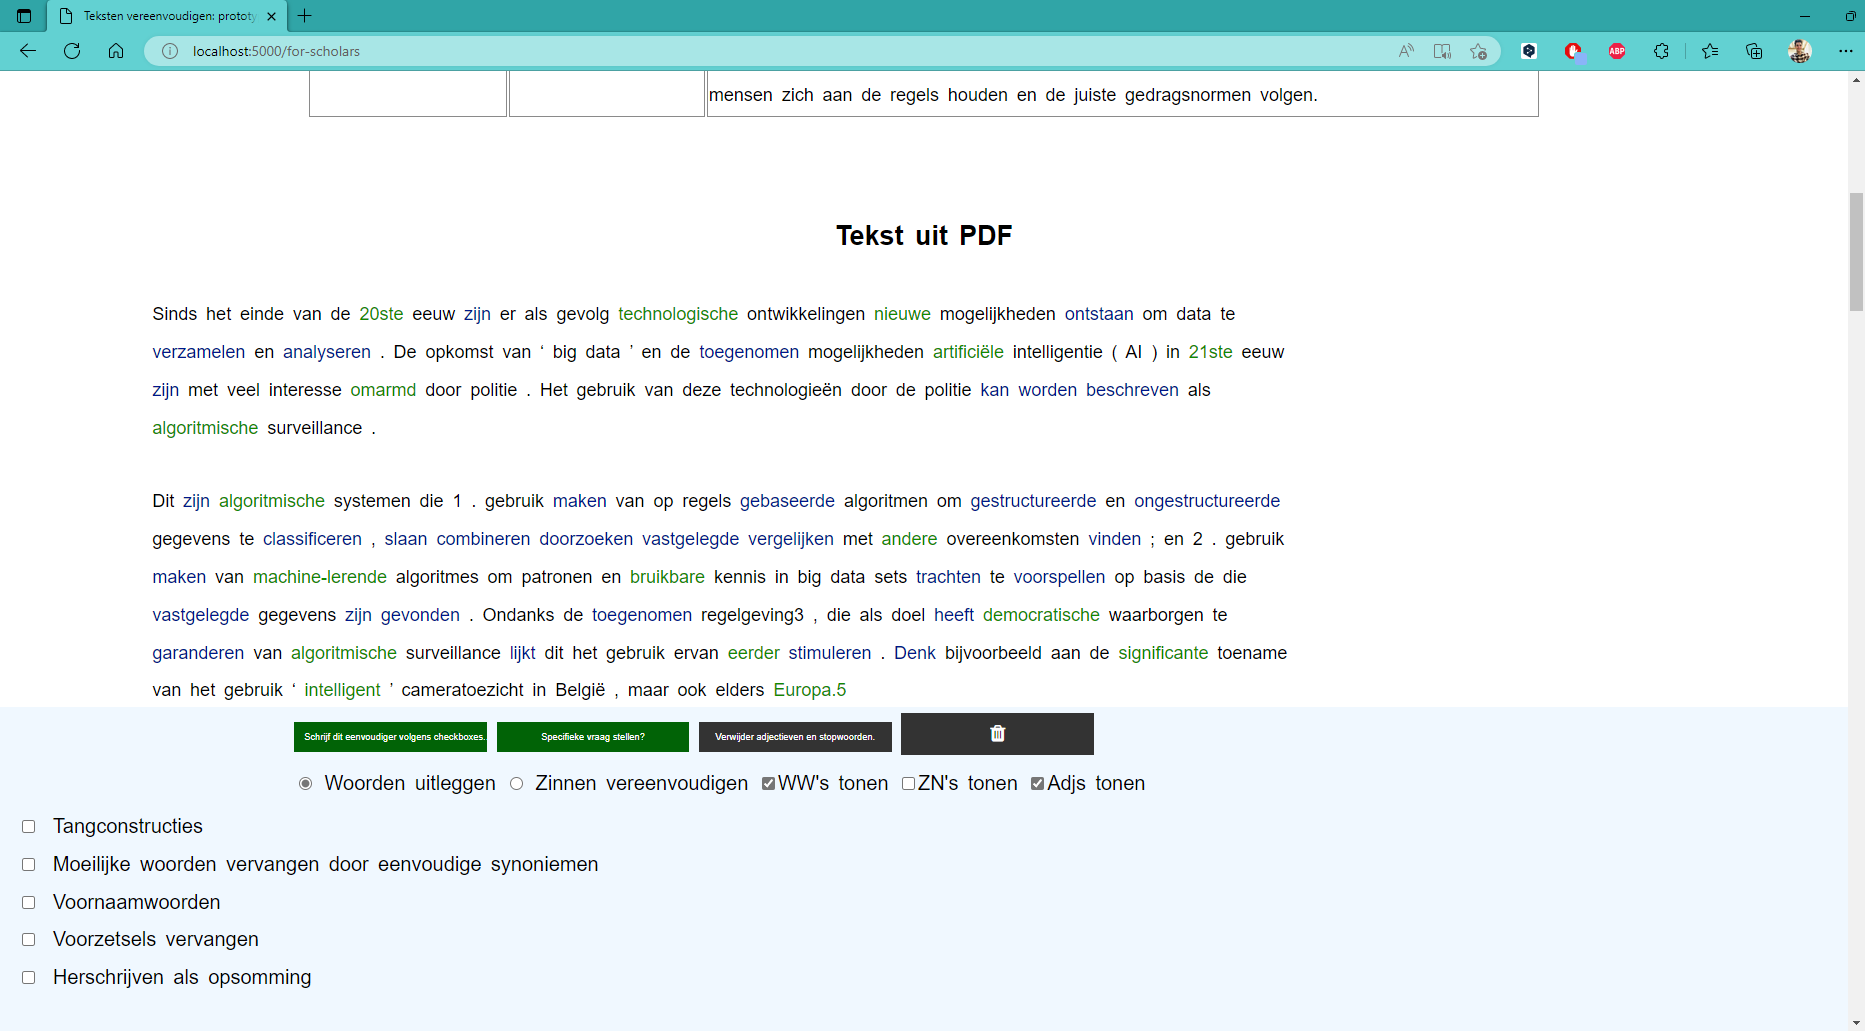
\includegraphics[width=\linewidth]{img/proto-pos-tagging.png}
		\caption{Een voorbeeldweergave van de toepassing van PoS-tagging bij het scholierencomponent.}
		\label{img:proto-pos-tagging-scholieren}
	\end{figure}
\end{center}

Scholieren kunnen zinnen selecteren om daarna deze tekst te laten vereenvoudigen met gepersonaliseerde ATS. Figuren \ref{img:proto-scholieren-step-1} en \ref{img:proto-scholieren-step-3} tonen hoe gebruikers met Pentimentor de gemarkeerde doorlopende tekst kunnen laten herschrijven naar een opsomming. Eerst markeren zij een stuk tekst om hiermee opties aan het mee te geven. Daarnaast kan het ook tekst herschrijven in een tabelformaat.

\begin{center}
	\begin{figure}[H]
		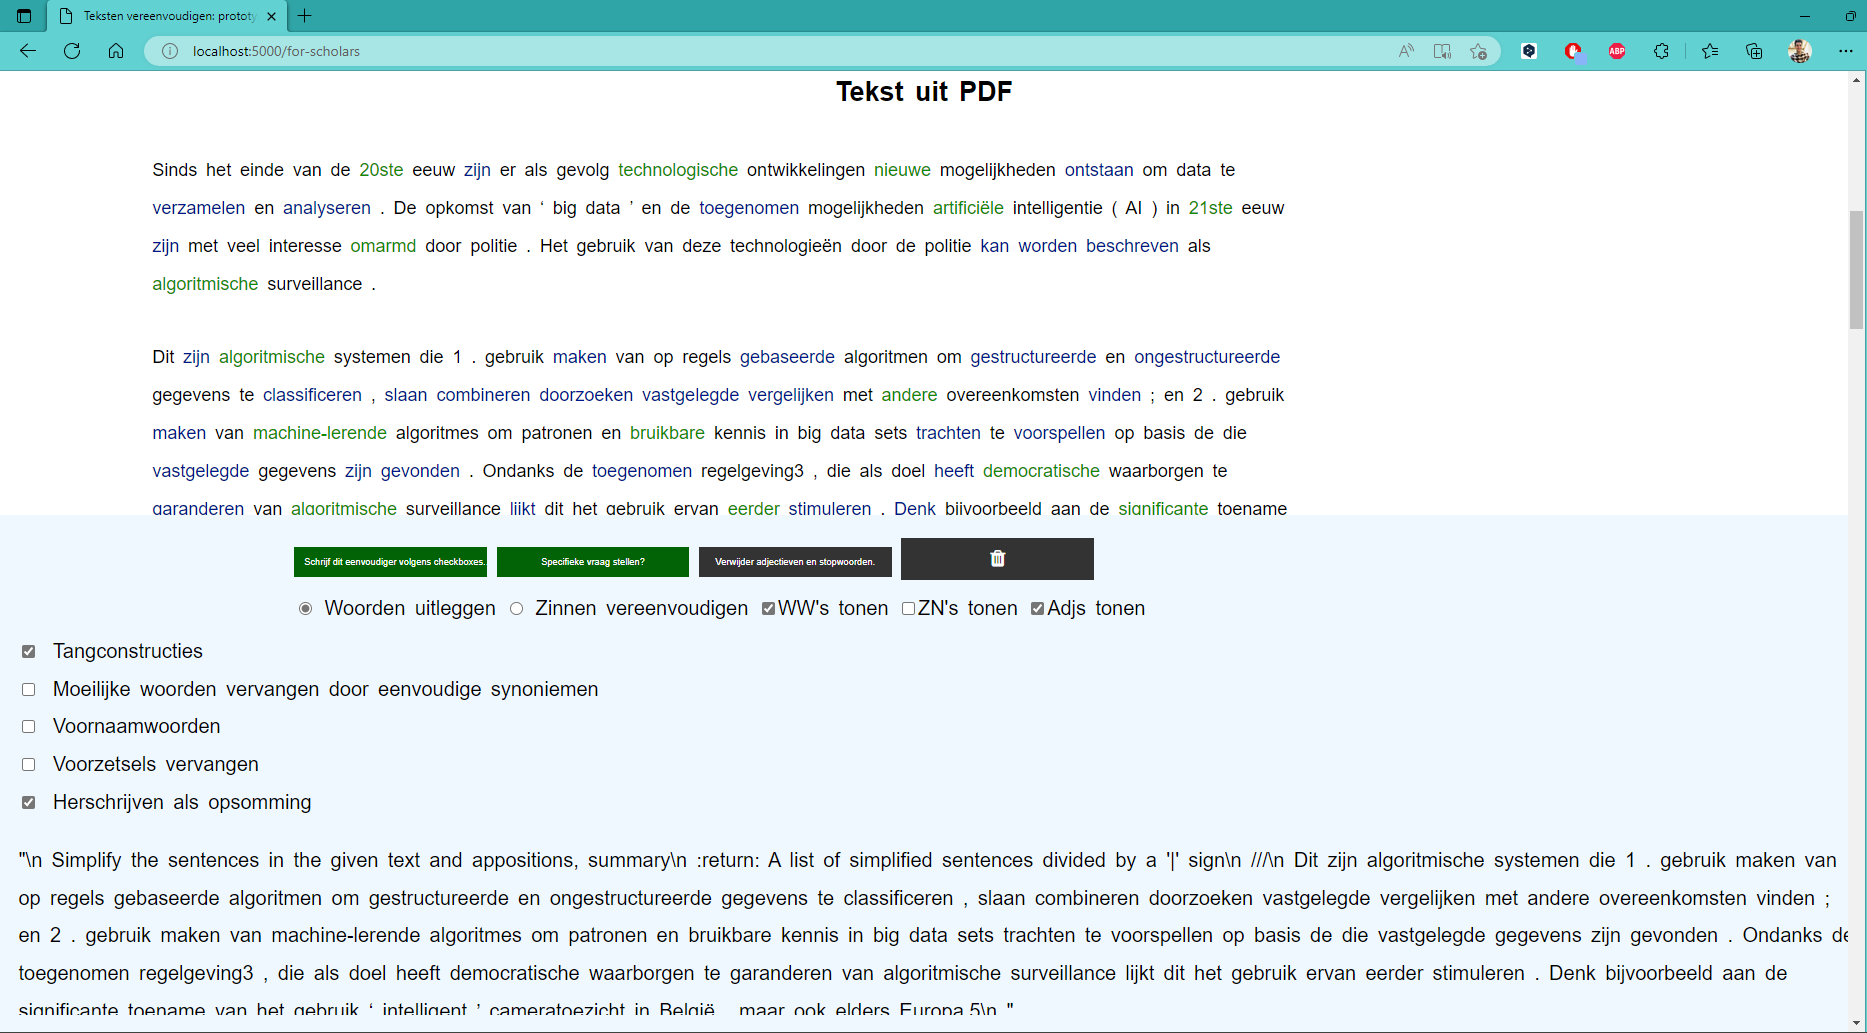
\includegraphics[width=\linewidth]{img/proto-opsomming-1.png}
		\caption{Stap 1 van een gepersonaliseerde tekstvereenvoudiging in het scholierencomponent.}
		\label{img:proto-scholieren-step-1}
	\end{figure}
\end{center}

\begin{center}
	\begin{figure}[H]
		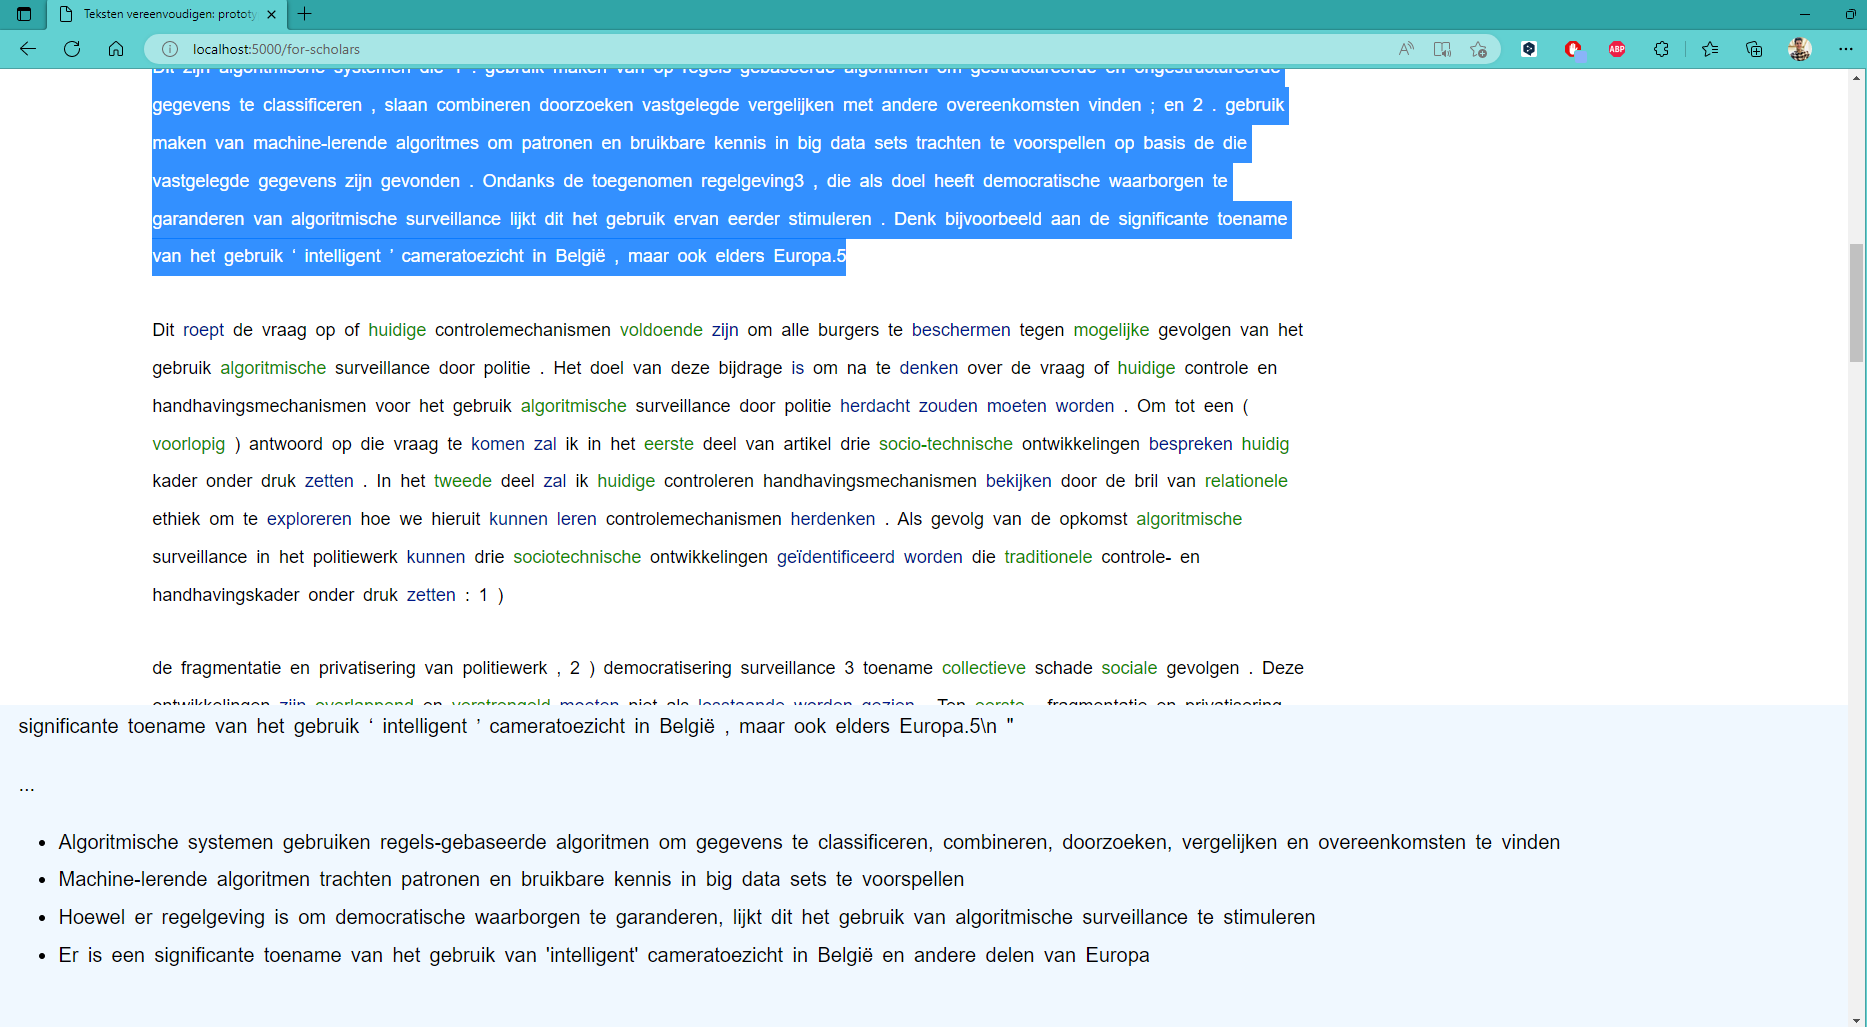
\includegraphics[width=\linewidth]{img/proto-opsomming-3.png}
		\caption{Stap 2 van een gepersonaliseerde tekstvereenvoudiging in het scholierencomponent.}
		\label{img:proto-scholieren-step-3}
	\end{figure}
\end{center}

Verder tonen figuren \ref{img:step-1-proto-vraagstelling} en \ref{img:step-2-proto-vraagstelling} een tweede functionaliteit. Zo kunnen scholieren specifieke vragen stellen aan Pentimentor door middel van een gecentreerd invoerscherm.

\begin{center}
	\begin{figure}[H]
		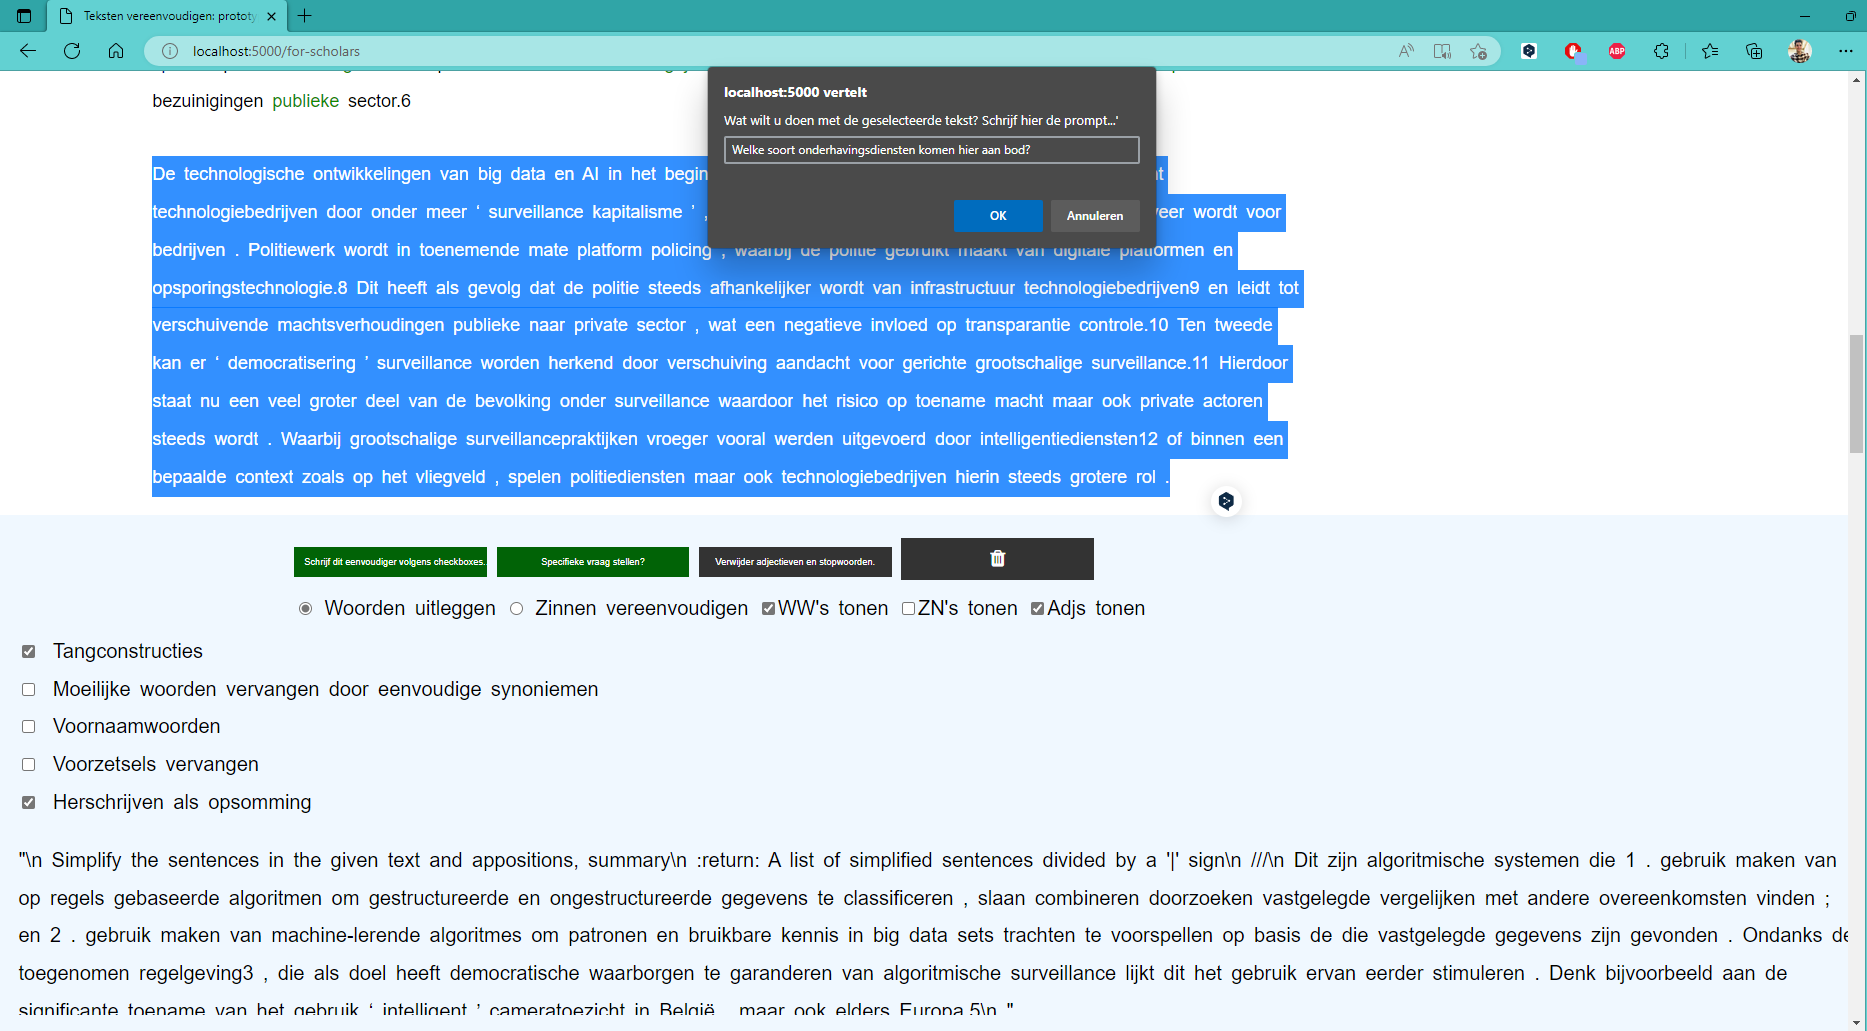
\includegraphics[width=\linewidth]{img/proto-vraagstelling-1.png}
		\caption{Stap 1 bij het stellen van een specifieke vraag bij gemarkeerde tekst.}
		\label{img:step-1-proto-vraagstelling}
	\end{figure}
\end{center}

\begin{center}
	\begin{figure}[H]
		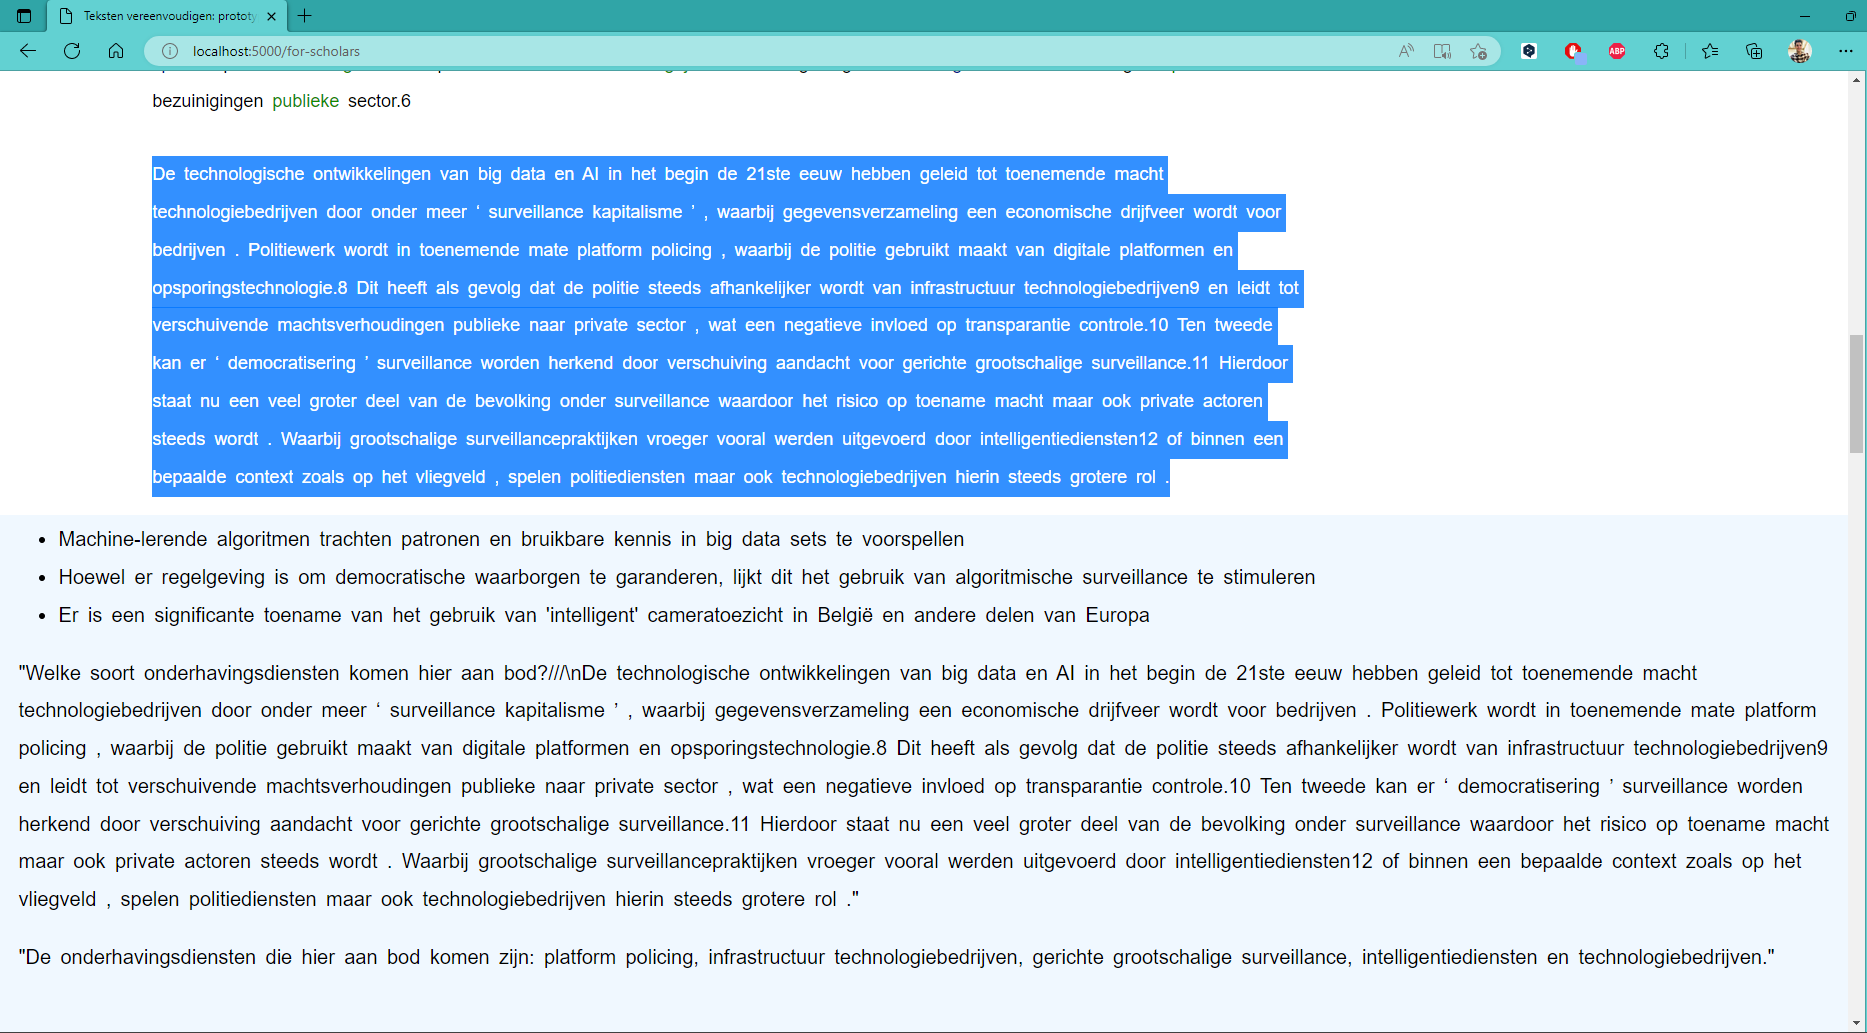
\includegraphics[width=\linewidth]{img/proto-vraagstelling-2.png}
		\caption{Stap 2 bij het stellen van een specifieke vraag bij gemarkeerde tekst.}
		\label{img:step-2-proto-vraagstelling}
	\end{figure}
\end{center}

Volgens de evaluatie en experimenten blijkt Pentimentor te voldoen aan de \textit{must-haves} uit de requirementsanalyse. Tabel \ref{img:moscow-table} geeft hier een overzicht van. Het biedt twee methoden aan om pdf-bestanden in te lezen. Dit via een pipeline van machineleer- en OCR-technieken. Bovendien kan het de tekst ophalen met behulp van PDFMiner, wat overeenkomt met de verwachte functionaliteiten voor pdf-upload. Daarnaast hebben gebruikers de vrijheid om te kiezen welke tekstinhoud ze willen vereenvoudigen met behulp van gepersonaliseerde ATS. Na de vereenvoudiging of samenvatting van een wetenschappelijk artikel kunnen eindgebruikers alle vragen beantwoorden met behulp van de inhoud van het vereenvoudigde artikel, zoals aangegeven door Hollenkamp (2020) als een absolute vereiste.

\medspace

Verder kunnen gebruikers de opmaak van Pentimentor aanpassen naargelang hun voorkeur. Zo past het systeem deze voorkeuren toe op de digitale weergave in de webtool, maar ook de opmaak van het uitvoerbestand. Figuur \ref{img:screenshot-pdf-attempt} toont de vereenvoudigde versie van het wetenschappelijke artikel met de parameters uit tabel \ref{table:chosen-parameters-experiment}. Daarnaast houdt Pentimentor rekening met de gekozen regeleindes, woord- en karakterspatiëring, lettertype -en grootte, koppenstructuur en marges van het uitvoerbestand. Pentimentor houdt hier rekening mee, in tegenstelling tot de andere uitgeteste toools. Enkel E1 en E2 kunnen het lettertype -en grootte aanpassen. Tot slot toont figuur \ref{img:screenshot-docx-attempt} hoe een volledig personaliseerbaar docx-bestand er uit kan zien.

\begin{figure}[H]
	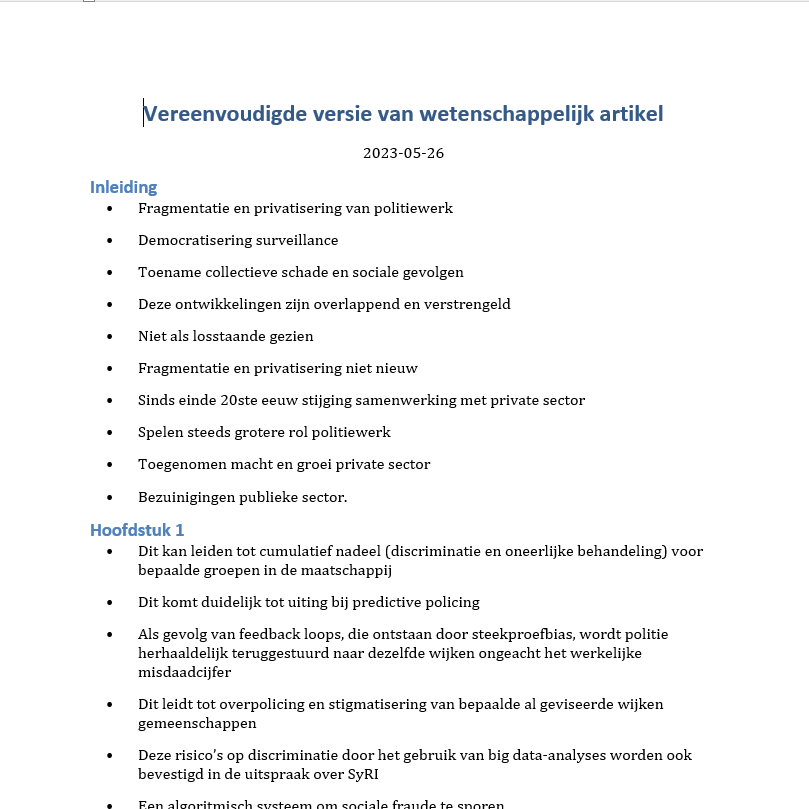
\includegraphics[width=\linewidth]{img/screenshot-prototype-word.png}
	\caption{De uitvoer na een vereenvoudiging met Pentimentor. De tekst is een vereenvoudigde versie van het artikel van \textcite{VanBrakel2022}.}
	\label{img:screenshot-docx-attempt}
\end{figure}

Verder bevat Pentimentor enkele \textit{should-haves}. Allereerst kunnen gebruikers een tekst op een duidelijke manier markeren. Hiermee kunnen zij annotaties toevoegen, de tekst aanpassen door \textit{in-line} definities toe te voegen. Bovendien kan Pentimentor abstraherende samenvattingen genereren in verschillende formaten, zoals opsommingen, tabellen of doorlopende tekst. Zo toont figuur \ref{img:screenshot-docx-attempt} een voorbeeld van een gegenereerde opsommingssamenvatting.

\medspace

Pentimentor zorgt voor een duidelijke gebruikerservaring door meldingsschermen te tonen wanneer het iets van de gebruiker verwacht. Figuur \ref{img:step-1-proto-vraagstelling} illustreert deze werking. Bovendien toont het waarschuwingen in formulieren, zoals getoond in figuur \ref{img:proto-lerarencomponent}.

\begin{figure}[H]
    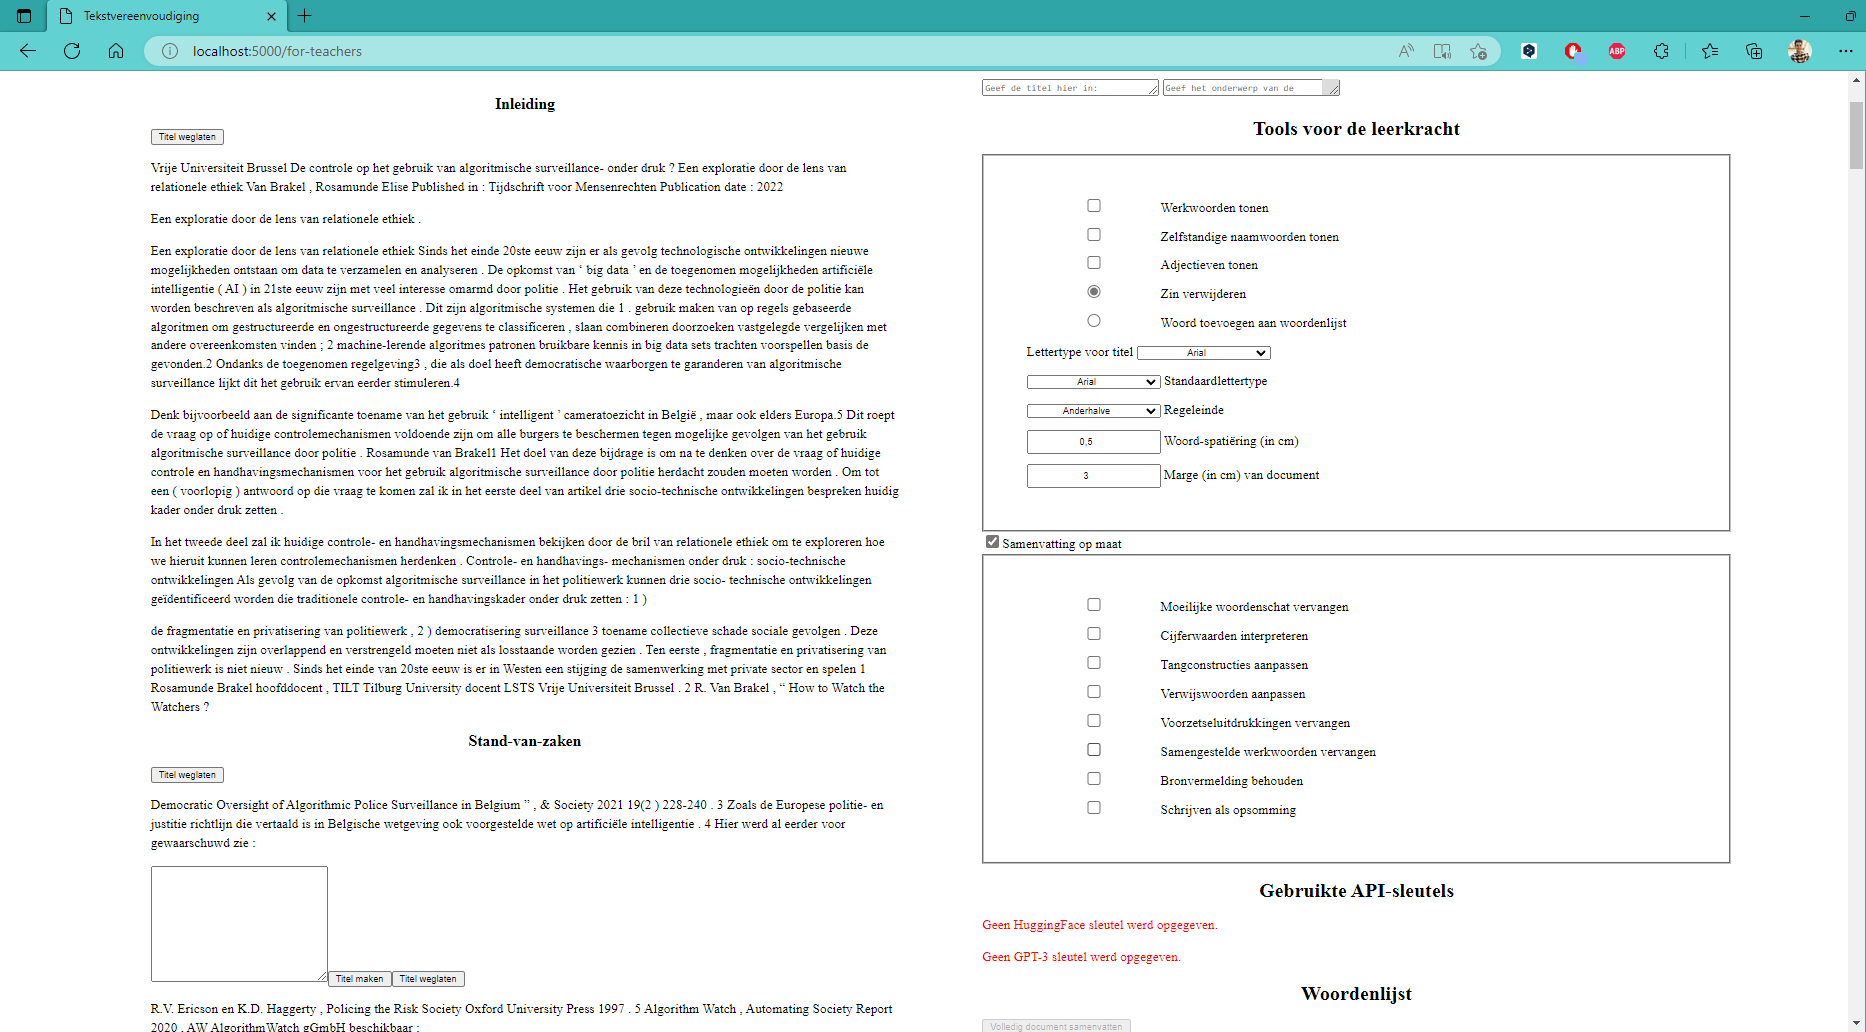
\includegraphics[width=\linewidth]{img/proto-lerarencomponent.png}
    \caption{Een mogelijke weergave van het lerarencomponent met het wetenschappelijk artikel van \textcite{VanBrakel2022} als input.}
    \label{img:proto-lerarencomponent}
\end{figure}

Echter voldoet Pentimentor niet aan alle \textit{should-haves}. Zo ontbreekt de mogelijkheid om automatisch een woordenlijst met moeilijke woorden of vakjargon te genereren. Daarnaast mist Pentimentor analytische functionaliteiten, zoals het tonen van tekstanalyse aan de eindgebruiker.

\medspace

Tot slot bevat Pentimentor geen \textit{wont-haves}. Zo ontbreekt het een luistercomponent waarmee scholieren de vereenvoudigde tekst kunnen beluisteren. Deze functionaliteit is wel aanwezig bij E1, E2 en E3. Andere uitgeteste tools beschikken hier ook niet over. Bovendien kunnen gebruikers Pentimentor alleen raadplegen in een lokale omgeving met Docker, terwijl zij wel andere geteste toepassingen zonder installatie kunnen raadplegen. Daarnaast heeft Pentimentor geen browserextensie, terwijl O5 dit als enige toepassing wel kan.
%%=============================================================================
%% Conclusie
%%=============================================================================

\chapter{Conclusie}%
\label{ch:conclusie}

Deze scriptie tracht een antwoord te bieden op de volgende onderzoeksvraag:

\begin{itemize}
	\item Hoe kan een wetenschappelijk artikel automatisch vereenvoudigd worden, gericht op de unieke noden van scholieren met dyslexie in de derde graad middelbaar onderwijs?
\end{itemize}

Eerst geeft de requirementsanalyse nieuwe inzichten in huidige toepassingen voor \textit{automatic text simplification} (ATS). Zo ontbreekt er personaliseerbaarheid in bestaande online tools. Verder beschikken tools die enkel lexicale vereenvoudiging toepassen over onvoldoende opmaakopties om de leeservaring van scholieren met dyslexie tijdens het begrijpend lezen van een wetenschappelijk artikel te bevorderen. Daarnaast kunnen eindgebruikers met deze toepassingen geen gepersonaliseerde vereenvoudiging of samenvatting maken. Ten slotte kunnen zij geen wetenschappelijke artikelen inladen in de toepassingen die wel gepersonaliseerde ATS kunnen uitvoeren. 

\medspace

Bing Chat en ChatGPT bieden mogelijkheden voor ATS aan. Ze vereisen echter een uitgebreide informaticakennis, ofwel een vaardigheid waarover de meeste scholieren en leraren niet beschikken. Ontwikkelaars kunnen de achterliggende taalmodellen gebruiken om toepassingen te maken, maar zij richten zich hoofdzakelijk op samenvattingstools. In hoofdzaak resulteert deze bijdrage niet in meer begrijpelijke teksten. Het komt het leerproces van scholieren vaak niet ten goede. Huidige toepassingen bewijzen nochtans dat ontwikkelaars toepassingen voor personaliseerbare tekstvereenvoudiging kunnen ontwikkelen. De opgestelde requirementsanalyse benadrukt de noodzaak van een gebruiksvriendelijke toepassing in het onderwijs, waarmee scholieren en leerkrachten wetenschappelijke teksten op een efficiënte manier kunnen vereenvoudigen.

\medspace

Vervolgens wijst de vergelijking van taalmodellen uit dat HuggingFace (HF) taalmodellen, specifiek getraind op vereenvoudigingsopdrachten, lexicale vereenvoudiging mogelijk maken. Het geavanceerde taalmodel GPT-3 doet het beter door bovendien syntactische vereenvoudiging aan te bieden, samen met formaatwijzigingen. Dit is ongezien bij huidige toepassingen. Zo produceert GPT-3 ook teksten met minder lange en complexe woorden. Dit taalmodel kan doelgroepen in grote lijn inschatten, waartoe andere tools niet in staat zijn. Geteste HF taalmodellen genereren minder coherente teksten en lopen het risico op samengesmolten zinnen. Daarnaast vereisen zij een extra vertaalfase, wat GPT-3 niet hoeft te doen. Zo moeten ontwikkelaars geen extra vertaalfase uitwerken wanneer zij teksten met GPT-3 willen vereenvoudigen. Daarbij moet het prototype specifieke prompts en technieken aangegeven door \textcite{McFarland2023, White2023} gebruiken.

\medspace

Tot slot toont de vorming van Pentimentor aan dat ontwikkelaars ATS-software kunnen ontwikkelen met \textit{open-source} AI- en NLP-technologieën. Zo kunnen zij PDFMiner en Layoutparser gebruiken om tekstinhoud uit wetenschappelijke artikelen te extraheren, met of zonder behoud van de oorspronkelijke titelstructuur. Bovendien kunnen ze de API van OpenAI's GPT-4 benutten voor gepersonaliseerde ATS-toepassingen door middel van geschikte prompts. Vervolgens kunnen zij met Pandoc gepersonaliseerde documenten in docx-formaat automatisch genereren. Ontwikkelaars kunnen basis Javascript toepassen om eenduidige handelingen voor eindgebruikers te onwikkelen, die voordien enkel per commandline mogelijk waren. Zo kunnen zij webpagina's opbouwen die voldoen aan de noden beschreven in \textcite{Rello2012a}.  Hoewel het prototype niet aan alle \textit{should-haves} en \textit{could-haves} voldoet, kunnen ontwikkelaars een volledig functionele toepassing uitwerken met de genoemde softwarepakketten.

\medspace

Dit onderzoek legt de nadruk op de aanwezigheid van geavanceerde taalmodellen en tools voor potentiële ATS-toepassingen die voldoen aan de behoeften van scholieren met dyslexie. GPT-3 kan dienen als een geschikt taalmodel, vanwege zijn sterke prestaties in toegepaste leesmetrieken, waaronder criteria zoals het aantal complexe en lange woorden per zin. Daarnaast kan dit taalmodel korte annotaties genereren voor vakjargon of onbekende woordenschat voor scholieren. Verder hebben ontwikkelaars de mogelijkheid om zich te richten op specifieke doelgroepen via aanpasbare parameters. Hierdoor kunnen teksten op maat worden gemaakt die aansluiten bij de individuele behoeften van de gebruiker. Ontwikkelaars moeten echter voorzichtig zijn met dergelijke toepassingen, omdat taalmodellen geen gegarandeerd correcte inschatting bieden voor de doelgroepen. Extra trainingsdata kan het model helpen bij deze inschatting door middel van leerstof op leesniveau van de doelgroep, zoals aangeraden door \textcite{Gooding2022}.
%%=============================================================================
%% Discussie
%%=============================================================================

\chapter{\IfLanguageName{dutch}{Discussie}{Discussie}}%
\label{ch:discussie}

Om te achterhalen hoe ontwikkelaars gepersonaliseerde \textit{automatic text simplification} (ATS) kunnen bieden, gebruikt het onderzoek drie onderzoeksmethoden. Het onderzoek focust enkel op ATS voor scholieren met dyslexie in de derde graad van het middelbaar onderwijs.

\medspace

Allereerst wijzen de resultaten van de requirementsanalyse uit dat zowel erkende toepassingen als online tools onvoldoende functionaliteiten bieden voor gepersonaliseerde ATS. Daarnaast bieden deze onvoldoende opmaakopties. Daarmee komt dit resultaat overeen met de verwachting dat ontwikkelaars hun toepassingen niet specifiek richten op ATS. Daarnaast komt het overeen met de verwachtingen dat ontwikkelaars geen rekening houden met scholieren met dyslexie in de derde graad van het middelbaar onderwijs bij deze tools. Hiervoor legt het onderzoek enkele verklaringen, onder andere de complexiteit die gepaard gaat met de ontwikkeling van dergelijk toepassing, het gebrek aan iniatief binnen het informaticavakgebied en de populariteit van samenvattingstools, zoals in de literatuurstudie aangegeven door \textcite{Gooding2022}.

\medspace

Hoewel de functionaliteiten van ChatGPT en Bing Chat mogelijke hulp bij gepersonaliseerde ATS kunnen aanbieden, ontbreken deze toepassingen de eenduidige handelingen waardoor gebruikers moeite kunnen hebben bij het handmatig vereenvoudigen van wetenschappelijke artikelen. Daarnaast houdt ChatGPT geen rekening met verwijzingen of artikelen buiten de getrainde data, wat de credibiliteit van de teruggekregen tekst kan verlagen. Daartegenover doet Bing Chat dat wel. Deze toepassing houdt rekening met externe referenties. Daarmee kunnen eindgebruikers snel teksten ophalen waarbij het systeem de referenties direct aan hen meegeeft. Ontwikkelaars kunnen deze toepassing of dergelijke API gebruiken om nauwkeurige toepassingen m referentiemateriaal aan te bieden in ondersteunende onderwijstoepassingen. Verder onderzoek naar de toepassing van deze AI via een API is noodzakelijk en kan baanbrekend zijn voor de onderwijssector, ondersteund door \textcite{Roose2023, Garg2022}. Anderzijds is er de mogelijkheid om bestaande toepassingen, zoals Kurzweil, uit te breiden met functionaliteiten die gepersonaliseerde ATS aanbieden aan scholieren met dyslexie in de derde graad van het middelbaar onderwijs. Tot slot moeten onderzoekers meer experimenten uitvoeren naar het gebruik van Bing Chat en ChatGPT in het onderwijs. 

\medspace

Bij de tweede onderzoeksmethode vergeleek het onderzoek vier verschillende \textit{pre-trained} taalmodellen. Deze onderzoeksfase wijst uit dat ontwikkelaars het GPT-3 taalmodel kunnen gebruiken voor gepersonaliseerde ATS. Zo maakte het geteste GPT-3 model de davinci-engine. Het onderzoek gaat niet verder dan het finetunen van de API-parameters. Zo bevat het geen extra tekstdata van wetenschappelijke artikelen. Verder wijst de vergelijkende studie uit dat de drie geteste HuggingFace (HF) taalmodellen en het geteste GPT-3 taalmodel via API beschikken over \textit{Complex Word Identification} (CWI)-functionaliteiten en \textit{substitution generation}. Hoewel de drie HF taalmodellen een gekregen tekst op lexicaal vlak kunnen vereenvoudigen, toch staan ze in de schaduw van GPT-3. Daarmee kan het GPT-3 taalmodel een baanbrekende oplossing bieden voor gepersonaliseerde ATS van wetenschappelijke artikelen, want het kan snel en efficiënt moeilijke woorden herkennen in doorlopende tekst. Tot slot kan het de oorspronkelijke tekst herschrijven als tabel of opsomming, wat huidige toepassingen niet aanbieden.

\medspace

Dit resultaat bevestigt de verwachting dat GPT-3 alle aspecten van gepersonaliseerde ATS kan aanbieden in tegenstelling tot de geteste HF taalmodellen die deze niet allemaal kan realiseren. Het onderzoek geeft de complexiteit van de getrainde data als mogelijke verklaring. Zo trainden de onderzoekers van de vier geteste taalmodellen deze specifiek op data van wetenschappelijke artikelen. Onderzoekers moeten deze verschillen verder onderzoeken. Zo kunnen zij de verschillen tussen de verschillende taalmodellen beter begrijpen, specifiek binnen de context van wetenschappelijke artikelen. Daarnaast kunnen \textit{Large Language Models} of LLM's ook prompts van ontwikkelaars beantwoorden. Deze taalmodellen kunnen verschillende antwoorden genereren, maar het onderzoek wijst uit dat ontwikkelaars de \textit{temperature} parameter kunnen aanpassen om één antwoord per prompt te verkrijgen. Hierover bestaat er onvoldoende onderzoek en daarom moet verder onderzoek zich richten op de verschillen tussen prompts en hun bijhorende \textit{temperature}. 

\medspace

Hoewel GPT-4 niet tot het onderzoek behoort, toch kunnen ontwikkelaars hiermee toepassingen maken. \textcite{Simon2021} geeft aan dat de verschillen tussen deze groei van het aantal parameters weinig effect hebben op de kwaliteit van de tekstdata. Toch beginnen ontwikkelaars snel de sprong te maken naar de volgende iteratie die ook meer energie van het systeem vereist. Verder onderzoek moet uitwijzen of de sprong van GPT-3 naar GPT-4 al dan niet merkbaar is op taalvlak. Een opvolgend onderzoek met dit taalmodel is vereist om te testen of dit taalmodel over voldoende data beschikt om wetenschappelijke artikelen te vereenvoudigen op maat van scholieren met dyslexie in de derde graad van het middelbaar onderwijs. 

\medspace

Vervolgens kunnen ontwikkelaars hun eigen specifieke prompts opstellen voor deze taalmodellen. Hierin kunnen zij ook de doelgroep meegeven en daarmee een extra parameter meegeven. Dit onderzoek bevestigt niet de mate waarin deze uitvoer verschilt van elkaar. Deze eenduidige oplossing kan echter een revolutionaire oplossing bieden voor gepersonaliseerde ATS of samenvatting. Daarom moeten onderzoekers hier verder onderzoek op uitvoeren. Verder onderzoek naar doelgroepinschattingen via prompts is ook nodig. Daarnaast zou toekomstig onderzoek zich kunnen richten op het potentieel van de combinatie van GPT-3 en \textit{full-text-search}-technologieën. 

\medspace

Verder stelt het onderzoek de gebruikte machinale beoordeling in vraag. Zo resulteerde de vereenvoudigde teksten door taalmodellen een miniem verschil bij de leesgraadscores FRE en FOG. Daarnaast wijst het experiment uit dat de \textit{readability}-library de actieve stem van een zin niet kan achterhalen. Daarom kan het onderzoek geen vaststelling maken of de taalmodellen van passief naar actief kunnen schrijven. Spacy \textit{word embeddings} kunnen een alternatieve techniek aanreiken om hulpwerkwoorden en vervoegingen van het werkwoord 'zijn' te achterhalen. Daarnaast kunnen toepassingen zoals TextInspector meer metrieken dan de uitgeteste leesgraadscores aanbieden. Daarom moeten onderzoekers verdere experimenten uitvoeren naar de bruikbaarheid van deze libraries. 

\medspace

De derde en laatste onderzoeksfase toont aan hoe ontwikkelaars toepassingen voor gepersonaliseerde ATS kunnen ontwikkelen. Dit specifiek op maat voor scholieren met dyslexie in de derde graad van het middelbaar onderwijs. Zo dienen de verworven kennis en aangeleerde tools uit de richtingen Toegepaste Informatica aan Vlaamse Hogescholen als startpunten om \textit{Pentimentor} te ontwikkelen. Hoewel Pentimentor slechts dient als een haalbaarheidstoetsing voor ontwikkelaars, toch moet de lezer rekening houden dat de ontwikkeling zich baseert op onderzochte kenmerken en technieken die de impact van handmatige tekstvereenvoudiging al hebben uitgewezen. Daarnaast gebeurt de ontwikkeling van Pentimentor met het oog op een eenduidige implementatie van technieken, die voordien enkel beschikbaar waren via CLI. Zo wijst de ontwikkeling van Pentimentor uit dat ontwikkelaars met vrij beschikbare middelen en API's wel dergelijk toepassingen kunnen maken. Dit resultaat komt overeen met de verwachting dat ontwikkelaars over de nodige tools beschikken. Zo baseert het onderzoek zich op de beschikbaarheid van \textit{open-source} tools en python-bibliotheken. Die stellen ontwikkelaars in staat om complexe taken eenvoudig te kunnen reproduceren. Hoewel Pentimentor aan alle vooropgestelde \textit{must-haves} voldoet, toch moet de lezer zich ervan bewust maken dat het doelpubliek niet werd opgenomen bij de testfase van Pentimentor. Daarom kan dit voornamelijk dienen als een haalbaarheidsmeting voor ontwikkelaars.

\medspace

Tot slot kunnen onderzoekers uit het logopedisch vakgebied Pentimentor gebruiken om onderzoek uit te voeren naar het leereffect op leesbegrip bij scholieren met dyslexie in de derde graad van het middelbaar onderwijs. Dit stemt overeen met de implicaties waar \textcite{Gooding2022} op wijst in haar onderzoek. Daarnaast moeten onderzoekers uit het onderwijsvakgebied de effecten van dergelijk tools observeren bij leerlingen en leerkrachten in het middelbaar onderwijs. Hoewel het onderzoek naar de bruikbaarheid van deze technologieën in het onderwijs zich in een prille fase bevindt, toch moeten onderzoekers de inzet van deze toepassingen verder onderzoeken. Deze bruikbaarheid kan via een browserextensie, lokale of online toepassing.



%---------- Bijlagen -----------------------------------------------------------

\appendix

\chapter{Onderzoeksvoorstel}

\section*{Samenvatting}

% Kopieer en plak hier de samenvatting (abstract) van je onderzoeksvoorstel.
Ingewikkelde woordenschat en zinsbouw hinderen scholieren met dyslexie in de derde graad van het middelbaar onderwijs bij het begrijpend lezen van wetenschappelijke artikelen. Gepersonaliseerde \textit{automated text simplification} (ATS) helpt deze scholieren bij hun leesbegrip. Daarnaast kan artificiële intelligentie (AI) dit proces automatiseren om de werkdruk bij leraren en scholieren te verminderen. Dit onderzoek achterhaalt met welke technologische en logopedische aspecten AI-ontwikkelaars rekening moeten houden bij de ontwikkeling van een AI-toepassing voor geautomatiseerde en gepersonaliseerde tekstvereenvoudiging. Hiervoor is de volgende onderzoeksvraag opgesteld: "Hoe kan een wetenschappelijk artikel automatisch worden vereenvoudigd, gericht op de unieke noden van scholieren met dyslexie in het derde graad middelbaar onderwijs?" . Een requirementsanalyse achterhaalt de benodigde functionaliteiten om gepersonaliseerde en geautomatiseerde tekstvereenvoudiging mogelijk te maken. Vervolgens wijst de vergelijkende studie uit welk taalmodel ontwikkelaars kunnen inzetten om de taak van gepersonaliseerde en geautomatiseerde tekstvereenvoudiging mogelijk te maken. De requirementsanalyse wijst uit dat toepassingen om wetenschappelijke artikelen te vereenvoudigen, gemaakt zijn voor een centrale doelgroep en geen rekening houden met de unieke noden van een scholier met dyslexie in het derde graad middelbaar onderwijs. Toepassingen voor gepersonaliseerde ATS zijn mogelijk, maar ontwikkelaars moeten meer inzetten op de unieke noden van deze scholieren.

% Verwijzing naar het bestand met de inhoud van het onderzoeksvoorstel
%---------- Inleiding ---------------------------------------------------------

\section{Introductie}%
\label{sec:introductie}

% Met een jaarlijks budget van 32 miljoen in het vakgebied kunstmatige intelligentie (AI) op de werkvloer is België een pionier \autocite{Crevits2022}.  Zo zijn er verschillende projecten, om taalgerelateerde AI-ontwikkelingen op te starten, uit de grond gestampt. Het amai!-project \footnote{https://amai.vlaanderen/}  verenigt AI-softwarebedrijven uit verschillende domeinen om zo met AI-toepassingen te maken die processen automatiseren om de werkdruk te verminderen, zoals binnen het onderwijs \textit{real-time} ondertiteling en een taalassistent voor leerkrachten in meertalige klasgroepen.

Het Vlaams middelbaar onderwijs staat op barsten. Werkdruk en stress overspoelen leraren en scholieren. Bovendien is de derde graad van het middelbaar onderwijs een belangrijke mijlpaal voor de verdere loopbaan van scholieren, al hebben zij volgens \textcite{Dapaah2022} dan moeite om grip te krijgen op de vakliteratuur bij STEM-vakken. De STEM-agenda\footnote{https://www.vlaanderen.be/publicaties/stem-agenda-2030-stem-competenties-voor-een-toekomst-en-missiegericht-beleid} van de Vlaamse overheid moet het STEM-onderwijs tegen 2030 aantrekkelijker te maken, door de ondersteuning voor zowel leerkrachten als scholieren te verbeteren. Toch neemt deze agenda de aanpak van steeds complexere wetenschappelijke taal, zoals beschreven in \textcite{Barnett2020}, niet op. Wetenschappelijke artikelen vereenvoudigen, op maat van de noden van een scholier met dyslexie in het middelbaar onderwijs, is tijds- en energie-intensief voor leerkrachten en scholieren. Automatische en adaptieve tekstvereenvoudiging biedt hier een baanbrekende oplossing om de werkdruk in het middelbaar onderwijs te verminderen.

Het doel van dit onderzoek is om te achterhalen met welke technologische en logopedische aspecten AI-ontwikkelaars rekening moeten houden bij de ontwikkeling van een adaptieve AI-toepassing voor geautomatiseerde tekstvereenvoudiging. De volgende onderzoeksvraag is opgesteld: "Hoe kan een wetenschappelijk artikel automatisch vereenvoudigd worden, gericht op de verschillende behoeften van scholieren met dyslexie in de derde graad middelbaar onderwijs?". Een antwoord op volgende deelvragen kan de onderzoeksvraag vereenvoudigen. Eerst geeft de literatuurstudie een antwoord op de eerste vier deelvragen. Daarna vormt het veldonderzoek een antwoord op de vijfde deelvraag. Ten slotte beantwoordt de vergelijkende studie de zesde en laatste deelvraag. De resultaten van dit onderzoek zetten AI-ontwikkelaars aan om een toepassing te maken om scholieren met dyslexie te kunnen ondersteunen in de derde graad middelbaar onderwijs.

% wat wordt manueel gedaan? --> voor de doelgroep
 % --> kleiner prototype
  
% aantal deelvragen doet er niet toe, maak gewoon dat je concrete en doelgerichte deelvragen hebt

\begin{enumerate}
	\item Welke aanpakken zijn er voor geautomatiseerde tekstvereenvoudiging? Aansluitende vraag: "Hoe worden teksten handmatig vereenvoudigd voor scholieren met dyslexie?"
	\item Welke specifieke noden hebben scholieren van de derde graad middelbaar onderwijs bij het begrijpen van complexere teksten?
	\item Wat zijn de specifieke kenmerken van wetenschappelijke artikelen? 
	\item Met welke valkuilen bij taalverwerking met AI moeten ontwikkelaars rekening houden?
	\item Welke toepassingen, tools en modellen zijn er beschikbaar om Nederlandstalige geautomatiseerde tekstvereenvoudiging met AI mogelijk te maken?
	\item Welke functies ontbreken AI-toepassingen om geautomatiseerde én adaptieve tekstvereenvoudiging mogelijk te maken voor \newline scholieren met dyslexie in de derde graad \newline middelbaar onderwijs? Aansluitende vraag: "Welke manuele methoden voor tekstvereenvoudiging komen niet in deze tools voor?"
\end{enumerate}

%---------- Stand van zaken ---------------------------------------------------

\section{State-of-the-art}%
\label{sec:state-of-the-art}

\subsection{Tekstvereenvoudiging}

% Deelvraag: Wat is tekstsimplificatie
De voorbije tien jaar is artificiële intelligentie (AI) sterk verder ontwikkeld. \textcite{Vasista2022} benadrukt dat de toename in kennis voor nieuwe toepassingen zorgde. Tekstvereenvoudiging vloeide hier uit voort. Momenteel bestaan er al robuuste toepassingen die teksten kunnen vereenvoudigen, zoals Resoomer\footnote{https://resoomer.com/nl/}, Paraphraser\footnote{https://www.paraphraser.io/nl/tekst-samenvatting} en Prepostseo\footnote{https://www.prepostseo.com/tool/nl/text-summarizer}. Binnen het kader van tekstvereenvoudiging is er bestaande documentatie beschikbaar waar onderzoekers het voordeel van toegankelijkheid aanhalen, maar volgens \textcite{Gooding2022} ontbreken deze toepassingen de extra noden die scholieren met dyslexie in de derde graad middelbaar onderwijs vereisen.

\textcite{Shardlow2014} haalt aan dat het algemene doel van tekstvereenvoudiging is om ingewikkelde bronnen toegankelijker te maken. Het zorgt voor verkorte teksten zonder de kernboodschap te verliezen. \textcite{Siddharthan2014} haalt verder aan dat tekstvereenvoudiging op één van drie manieren gebeurt. Er is conceptuele vereenvoudiging waarbij documenten naar een compacter formaat worden getransformeerd. Daarnaast is er uitgebreide modificatie die kernwoorden aanduidt door gebruik van redundantie. Als laatste is er samenvatting die documenten verandert in kortere teksten met alleen de topische zinnen. Met deze concepten zijn ontwikkelaars volgens \textcite{Siddharthan2014} in staat om ingewikkelde woorden te vervangen door eenvoudigere synoniemen of zinnen te verkorten zodat ze sneller leesbaar zijn.

Tekstvereenvoudiging behoort tot de zijtak van \textit{Natural Language Processing} (NLP) in AI. NLP omvat methodes om menselijke teksten om te zetten in tekst voor machines. Documenten vereenvoudigen met NLP kan volgens \textcite{Chowdhary2020} op twee manieren: extraherend of abstraherend. Bij extraherende vereenvoudiging worden zinnen gelezen zoals ze zijn neergeschreven. Vervolgens bewaart een document de belangrijkste taalelementen om de tekst te kunnen hervormen. Deze vorm van tekstvereenvoudiging komt volgens \autocite{Sciforce2020} het meeste voor. Daarnaast is er abstraherende vereenvoudiging waarbij de kernboodschap wordt bewaard. Met de kernboodschap wordt er een nieuwe zin opgebouwd. Volgens het onderzoek van \textcite{Chowdhary2020} heeft deze vorm potentieel, maar het zit nog in de kinderschoenen.

\subsection{Noden van scholieren met dyslexie}

% Deelvraag 2: Bewezen voordelen van tekstsimplificatie bij scholieren met dyslexie
Het experiment van Franse wetenschappers \newline \textcite{Gala2016} illustreert dat manuele tekstvereenvoudiging schoolteksten toegankelijker \newline maakt voor kinderen met dyslexie. Dit deden ze door simpelere synoniemen en zinsstructuren te gebruiken. Tien kinderen werden opgenomen in het experiment, variërend van 8 tot 12 jaar oud. Verwijswoorden werden vermeden en woorden kort gehouden. De resultaten waren veelbelovend. Het leestempo lag hoger en de kinderen maakten minder leesfouten. Ook bleek er geen verlies van begrip in de tekst bij geteste kinderen. Resultaten van de studie werden gebundeld voor de mogelijke ontwikkeling van een AI-tool.

% doelgroep concreter maken hierboven
% semantisch vlak --> zinsstructuur
% welke criteria vonden zij 'geslaagd'?

De visuele weergave van tekst beïnvloedt de leessnelheid bij scholieren met dyslexie. Zo haalt het onderzoek van \textcite{Rello2012} tips aan waarmee teksten en documenten rekening moeten houden bij scholieren met dyslexie in de derde graad middelbaar onderwijs. Het gaat over speciale lettertypes, spreiding tussen woorden en het gebruik van inzoomen op aparte zinnen. Het onderzoek haalt verder aan dat teksten voor deze unieke noden aanpassen tijdrovend is en daarmee tekstvereenvoudiging door AI een revolutionaire oplossing kan bieden. De Universiteit van Kopenhagen is met bovenstaande idee aan de slag gegaan. Onderzoekers \textcite{Bingel2018} hebben gratis software ontwikkeld, genaamd Hero\footnote{https://beta.heroapp.ai/}, om tekstvereenvoudiging voor scholieren in het middelbaar onderwijs met dyslexie te automatiseren. De software bestudeert met welke woorden de gebruiker moeite heeft, en vervangt die door simpelere alternatieven. Hero bevindt zich nu in beta-vorm en wordt enkel in het Engels en Deens ondersteund. Als alternatief is er Readable\footnote{https://readable.com/}. Dit is een Engelstalige AI-toepassing dat zinnen beoordeeld met leesbaarheidsformules.

% Deelvraag: Uitdagingen van AI-software met tekstsimplificatie
\textcite{Roldos2020} haalt aan dat NLP in de laatste decennia volop in ontwikkeling is, maar ontwikkelaars botsen nog op uitdagingen. Het gaat om zowel interpretatie- als dataproblemen bij AI-modellen. Het onderzoek haalt twee punten aan. Allereerst is het voor een machine moeilijk om de context van homoniemen te achterhalen. Bijvoorbeeld bij het woord ‘bank’ is het niet duidelijk voor de machine of het gaat over de geldinstelling of het meubel. Daarnaast zijn synoniemen een probleem voor tekstverwerking.

Het onderzoek van \textcite{Sciforce2020} haalt aan dat het merendeel van NLP-toepassingen Engelstalige invoer gebruikt. Niet-Engelstalige toepassingen zijn zeldzaam. De opkomst van AI technologieën die twee datasets gebruiken, biedt een oplossing voor dit probleem. De software vertaalt eerst de oorspronkelijke tekst naar de gewenste taal, voordat de tekst wordt herwerkt. Hetzelfde onderzoek bewijst dat het vertalen van gelijkaardige talen, zoals Duits en Nederlands, een minimaal verschil opleverd.

% Deelvraag: Stand van zaken bij Belgische secundaire scholen
% Voor scholieren met dyslexie in het derde graad middelbaar onderwijs bestaan digitale hulpmiddelen die voor een betere visuele presentatie zorgen van teksten. De Vlaamse overheid leent gratis abonnementen\footnote{https://onderwijs.vlaanderen.be/nl/onderwijspersoneel/van-basis-tot-volwassenenonderwijs/lespraktijk/ict-in-de-klas/voorleessoftware-voor-leerlingen-met-leesbeperkingen} uit voor voorlees- en schrijfsoftware. De voornaamste zijn SprintPlus\footnote{https://www.sprintplus.be/}, Alinea\footnote{https://sensotec.be/product/alinea-suite/} en Kurzweil3000\footnote{https://sensotec.be/product/kurzweil-3000/}. Vlaamse scholieren met dyslexie in het middelbaar onderwijs kunnen voor deze software een gratis abonnement of licentie aanvragen. Al bieden de vijf softwarepakketten elk een samenvattingsfunctie aan, echter ligt de focus op spreek- en luisterfuncties waarbij het samenvatten en markeren van tekst als extra wordt gehouden.

% \subsection{Wetenschappelijke artikelen}

Volgens \textcite{PlavenSigray2017} houden onderzoekers zich vaak in hun eigen taalbubbel, wat negatieve gevolgen heeft voor de leesbaarheid van een wetenschappelijk artikel. Bovendien vormt de stijgende trend van het gebruik aan acroniemen \textcite{Barnett2020} een extra hindernis. \textcite{Donato2022} haalt aan dat onbegrijpelijke literatuur, waaronder studiemateriaal geschreven door de docent en online wetenschappelijke artikelen, één van de redenen is waarom scholieren met dyslexie in het middelbaar onderwijs van richting veranderen.

\subsection{Huidige toepassingen}

Vlaanderen heeft weinig zicht op de geïmplementeerde AI software in scholen. Dit werd vastgesteld door \autocite{Martens2021}, een samenwerking tussen de Vlaamse universiteiten en overheid voor AI. Vergeleken met andere Europese landen, maakt België het minst gebruik van leerling-georiënteerde hulpmiddelen. Degenen die wel gebruikt worden, zijn vooral online leerplatformen voor zelfstandig werken. Ook maakt België amper gebruik van beschikbare software die de leermethoden en -noden van leerlingen evalueert \autocite{Martens2021a}. 

\textcite{Verhoeven2023} haalt aan dat AI-toepassingen zoals ChatGPT, Google Bard en Bing AI kunnen helpen om routinematig werk te verminderen in het onderwijs. Echter haalt \textcite{Deckmyn2021} aan dat GPT-3, het model van ChatGPT, sterker staat in het maken van Engelstalige teksten vergeleken met Nederlandstalige teksten. De databank waar het GPT-3 model mee is getraind, bestaat uit 92\% Engelstalige woorden, terwijl er 0,35\% Nederlandse woorden aanwezig zijn in dezelfde databank. Ontwikkelaars moeten de evolutie van deze modellen opvolgen, voordat er Nederlandstalige toepassingen mee worden gemaakt.

% eventueel Bing AI bekijken
% --> artikel: 

% Deelvraag: Wat is er nodig voor tekstsimplificatie? 

\subsection{Ontwikkelen met AI}

Python staat bovenaan de lijst van programmeertalen voor NLP-toepassingen. Volgens het onderzoek van \textcite{Thangarajah2019} is dit te wijten aan de eenvoudige syntax, kleine leercurve en grote beschikbaarheid van kant-en-klare bibliotheken. Wiskundige berekeningen of statistische analyses kunnen worden uitgevoerd met één lijn code. \textcite{Malik2022} haalt de twee meest voorkomende aan, namelijk NLTK\footnote{https://www.nltk.org/} en Spacy\footnote{https://spacy.io/}. \textit{Deep Martin}\footnote{https://github.com/chrislemke/deep-martin} bouwt verder op het onderzoek van \textcite{Shardlow2014} naar een pipeline voor lexicale vereenvoudiging. \textit{Deep Martin} maakt gebruik van \textit{custom transformers} om invoertekst te converteren naar een vereenvoudigde versie van de tekstinhoud.

Voor Germaanse talen zijn er enkele datasets en word embeddings beschikbaar die de complexiteit van woorden bijhouden. Zo zijn er in de Duitse taal Klexicon\footnote{https://github.com/dennlinger/klexikon} en TextComplexityDE\footnote{https://github.com/babaknaderi/TextComplexityDE}. Een onderzoek van \textcite{Suter2016} bouwde een rule-based NLP-model met 'Leichte Sprache', wat een dataset is met eenvoudige Duitstalige zinsconstructies. Nederlandstalige datasets zijn in schaarse hoeveelheden beschikbaar, waardoor het vertalen uit een Germaanse taal is hier een optie.

Volgens \textcite{Garbacea2021} is het belangrijk dat AI-ontwikkelaars niet alleen aandacht besteden aan het aanpassen van woorden en zinnen, maar ook aan de gebruiker meegeven waarom iets is aangepast. De onderzoekers wijzen op twee ethische aspecten. Eerst moet de toepassing duidelijk aangeven waarom een woord of zin is aangepast. Het model moet de moeilijkheidsgraad van de woorden of zinnen bewijzen. \textcite{Iavarone2021} beschrijft een methode met regressiemodellen om de moeilijkheidsgraad te bepalen door een gemiddeld moeilijkheidspercentage per zin te berekenen. Daarnaast benadrukt \textcite{Garbacea2021} het belang van het markeren van de complexere delen van een tekst. Hiervoor haalt hetzelfde onderzoek methoden aan zoals \textit{lexical} of \textit{deep learning}.

Er is een tactvolle aanpak nodig om een vereenvoudigde tekst met AI te beoordelen. De studie van \textcite{Swayamdipta2019} haalt aan dat er extra nood is aan NLP-modellen waarbij de tekst zijn kernboodschap behoudt. Samen met Microsoft Research bouwden ze NLP-modellen die gericht waren op de bewaring van zinsstructuur en -context door \emph{scaffolded learning}. Hiervoor maakten de onderzoekers gebruik van een voorspellingsmethode die de positie van woorden en zinnen in een document beoordeelde. De Flesch-Kincaid leesbaarheidstest is volgens \newline \textcite{Readable2021} een alternatieve manier om vereenvoudigde tekstinhoud te beoordelen, zonder de nood aan \textit{pre-trained} modellen. Figuur \ref{img:readable-scheme} geeft de indeling per doelgroep weer. Deze score kan eenvoudig worden berekend met de \textit{Python-library} \textit{textstat}\footnote{https://pypi.org/project/textstat/}. 

\begin{figure}
	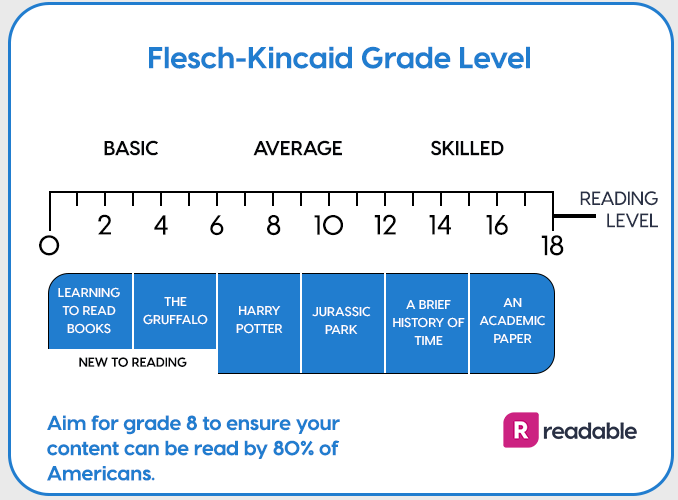
\includegraphics[width=\linewidth]{img/Screenshot_302.png}
	\caption{De indeling van leesgraadscores per doelgroep. Bron: \autocite{Readable2021}}
	\label{img:readable-scheme}
\end{figure}

%---------- Methodologie ------------------------------------------------------
\section{Methodologie}%
\label{sec:methodologie}
Een \textit{mixed-methods} onderzoek toont aan hoe toepassingen automatisch een wetenschappelijke artikel kunnen vereenvoudigen, gericht op scholieren met dyslexie in de derde graad middelbaar onderwijs. Het onderzoek houdt vijf grote fases in. De eerste fase is het proces van geautomatiseerde tekstvereenvoudiging beschrijven. Dit gebeurt via een grondige studie van vakliteratuur en wetenschappelijke teksten. Ook blogs van experten komen hier aan bod. Na het verwerven van de nodige inzichten wordt er een verklarende tekst opgesteld.

De tweede fase bestaat uit het analyseren van wetenschappelijke werken over de bewezen voordelen van tekstvereenvoudiging bij scholieren met dyslexie van de derde graad middelbaar onderwijs. Hiervoor zijn geringe thesissen beschikbaar, die zorgvuldigheid vragen tijdens interpretatie. De resulterende tekst bevat de voordelen samen met hun wetenschappelijke onderbouwing.

De derde fase is opnieuw een beschrijving. Hier worden de valkuilen bij taalverwerking met AI-software nagegaan. Deze fase van het onderzoek brengt mogelijke nadelen en tekortkomingen van AI-software bij tekstvereenvoudiging aan het licht. Dit gebeurt aan de hand van een technische uitleg.

De vierde fase omvat een toelichting over beschikbare AI toepassingen voor tekstvereenvoudiging. Aan de hand van een veldonderzoek op het internet en bij bedrijven wordt een longlist opgesteld van beschikbare toepassingen voor tekstvereenvoudiging in het middelbaar onderwijs. Met een requirementsanalyse wordt er een shortlist opgesteld van software. Het toetsen van verschillende tools wordt ook betrokken in deze fase. De shortlist vormt de basis voor de ontwikkeling van een prototype voor geautomatiseerde en adaptieve tekstvereenvoudiging.

% bestaande technologie gebruiken
% multilinguale modellen --> Nederlands als brugtaal
% hoe testen? --> output van specifieke tools
% trials --> selectie van maken --> als ik 'dit' toepas, dan krijg ik 'dit'

% tool van nieuwsbrieven --> hoe ver staan zij?
% --> interessant om te zien waar de parallellen liggen: complexe zinnen, woorden

De vijfde en laatste fase van het onderzoek bestaat uit het testen en beoordelen van gekozen AI-toepassingen voor tekstvereenvoudiging. In dit experiment proberen scholieren met dyslexie in de derde graad middelbaar onderwijs de shortlisted AI toepassingen en het prototype uit. Het doel van het experiment is om de effectiviteit en gebruikersvriendelijkheid van deze toepassingen te beoordelen. Na een grondige analyse wordt er met de resultaten bepaalt of de toepassingen aan de unieke noden van een scholier met dyslexie in de derde graad middelbaar onderwijs voldoen om wetenschappelijke artikelen te vereenvoudigen voor scholieren in het middelbaar onderwijs.

%---------- Verwachte resultaten ----------------------------------------------
\section{Verwacht resultaat, conclusie}
\label{sec:verwachte_resultaten}

% exclameren dat de tools goed automatiseren, maar weinig tot geen keuze aanreiken

Er wordt verwacht dat de huidige softwareoplossingen voor tekstvereenvoudiging onvoldoende aansluiten bij de noden van scholieren met dyslexie in de derde graad middelbaar onderwijs. Het prototype is moeilijk af te stemmen op de specifieke noden van deze doelgroep. Ontwikkelaars die werken met bestaande modellen moeten \textit{custom transformers} inzetten om bevredigende resultaten te krijgen. Bovendien ontbreken er Nederlandstalige word embeddings die de complexiteit van elk woord bijhouden en aan kant-en-klare modellen die de inhoud van wetenschappelijke artikelen kunnen vereenvoudigen. Word embeddings uit een Germaanse taal gebruiken, gevolgd door vertaling naar het Nederlands is wel een aanvaardbaar alternatief. 

% Er zijn te weinig kant-en-klare algoritmen en modellen beschikbaar om een pipeline voor tekstvereenvoudiging op te zetten, gericht op scholieren met dyslexie in het middelbaar onderwijs. 



%%---------- Andere bijlagen --------------------------------------------------
\chapter{Referentieteksten: Richtlijnen}
\label{ch:referentietekst}
	
Het onderzoek achterhaalt hoe scholieren met dyslexie in de derde graad middelbaar onderwijs ondersteund kunnen worden bij het intensief lezen van een wetenschappelijk artikel. De ondersteuning wordt aangeboden in de vorm van tekstvereenvoudiging met AI. Tekstvereenvoudiging omvat het lexicaal en syntactisch vereenvoudigen, alsook het samenvatten van de kerngedachte per hoofdstuk. Om tekstvereenvoudiging met AI te testen, moeten handmatig en automatisch vereenvoudigde teksten met elkaar worden vergeleken. 
	
	\medspace
	
De opdracht voor deze bijdrage is het manueel vereenvoudigen van een gekregen wetenschappelijk artikel. Dit wetenschappelijk artikel is zes pagina's (voorpagina uitgesloten) lang. Het doelpubliek voor dit vereenvoudigd artikel zijn scholieren met dyslexie in de derde graad ASO/TSO middelbaar onderwijs. Concreet zou dit een artikel moeten zijn dat tijdens een STEM-les wordt gegeven aan deze doelgroep. Op pagina 2 vindt u tekstvereenvoudigingstechnieken terug. Deze aanpassingen hebben een beneficieel effect op scholieren met dyslexie een wetenschappelijk artikel bij het intensief lezen van wetenschappelijke teksten. U dient deze gekregen aanpassingen te volgen voor deze bijdrage. De beschreven technieken en elementen dienen in de manuele vereenvoudigde tekst terug te vinden zijn. 
	
	\medspace
	
Op basis van de richtlijnen op pagina 2 worden dezelfde instructies aan een AI-model gegeven. Met de richtlijnen en de door u handmatig vereenvoudigde tekst kan het onderzoek evalueren of AI-taalmodellen capabel zijn om manuele tekstvereenvoudigingstechnieken, specifiek voor scholieren met dyslexie, toe te passen op wetenschappelijke artikelen. De tekst dat een AI-model vereenvoudigd wordt afgetoetst op basis van bestaande metrieken en de kenmerken van uw vereenvoudigde versie. % Woordenschat die in de eerste en tweede graad gekend zijn, hoeven niet aangepast te worden en wordt vernomen als 'gekend'. 
	
	\medspace
	
Voor de vereenvoudigde versie van het artikel moet u als taaldocent of auteur geen rekening houden met marges, lettertypes of spatiëring. Deze aanpassingen mogen, maar enkel de tekstuele inhoud van het gekregen document wordt in het experiment opgenomen. Een Word-document of PDF-document is voldoende. Daarnaast moet er ook geen rekening worden gehouden met de afbeeldingen in het artikel.  
	
	\medspace
	
Aanpassingen die niet op pagina 2 omschreven zijn om de tekst eenvoudiger te maken, zijn vrijblijvend. Indien deze aanpassing volgens u een meerwaarde biedt, dan moet de werkwijze voor de start van het document kort beschreven worden. De aanpassing moet eenmalig bovenaan het document worden vermeld. Bijvoorbeeld: 'De zin werd gesplitst omdat deze langer is dan tien woorden.' Zo kunnen wij bij het onderzoek rekening houden met deze extra handeling. Het AI-model wordt dan met deze extra parameter in het achterhoofd beoordeeld.
	
	\medspace
	
Namens mijn promotor, copromotors en mezelf wil ik u hartelijk bedanken voor uw interesse in dit onderzoek.
	
	\newpage
	
\section{Lexicale vereenvoudiging}
	
\begin{itemize}
	\item Een moeilijk woord achterhalen gebeurt op basis van intuïtie en inschatting van de doelgroep. De woordenschat die zelden voorkomt in de dagelijkse lees- en schrijftaal van STEM-vakken voor scholieren tussen 16 en 18 jaar oud, moet worden aangepast. Vakjargon die al in de tweede graad ASO en TSO aan bod is gekomen, mag behouden blijven.
	\item Een woord dat langer is dan achttien letters, wordt als moeilijk beschouwd en moet vervangen worden door een korter (en eenvoudiger) alternatief.
	\item Acroniemen worden voluit geschreven.
	\item Vervang een moeilijk woord in het artikel door slechts één synoniem. Bijvoorbeeld, als het woord 'adhesief' wordt vervangen door 'klevend', gebruik dan geen andere synoniemen voor 'klevend' in de rest van het artikel. 
	\item Indien een woord geen eenvoudiger synoniem heeft, mag het woord kort worden uitgelegd. Dit kan tussen ronde haakjes, of in een aparte zin. Bijvoorbeeld: "Ik voelde me melancholisch." wordt aangepast naar "Ik had een diep gevoel van droefheid en verlies.".		
		\item Vermijd het directe overnemen van percentages indien deze voorkomen in het artikel. Vervang dit door benamingen zoals 'een kwart', 'de helft'. 
	\end{itemize}
	
	\section{Syntactische vereenvoudiging}
	
	\begin{itemize}
		\item Te lange zinnen worden opgebroken of gesplitst. De zinnen in het vereenvoudigde artikel zijn hoogstens tien woorden lang.
		\item Verwijswoorden zoals 'zij', 'hun' of 'hij' worden naar namen veranderd. Bijvoorbeeld voornamen of entiteitsnamen (bijvoorbeeld Nationale Bank). 
		\item Tangconstructies worden vervangen. Dit kan door de bijzin naar het begin of het einde van een zin te plaatsen, de zin te splitsen in twee kortere zinnen of door het onderwerp en de persoonsvorm dichter bij elkaar te plaatsen door minder informatie tussenin te plaatsen.
		\item Voorzetseluitdrukkingen en samengestelde werkwoorden worden vervangen indien mogelijk. Indien er geen eenvoudigere alternatieven zijn, mogen deze onaangepast blijven.
	\end{itemize}
	
	\section{Structurele aanpassingen}
	
	\begin{itemize}
		\item Het vereenvoudigde artikel volgt dezelfde structuur en chronologische volgorde zoals dat van het oorspronkelijk artikel. Iedere hoofdstuk in het wetenschappelijk artikel is hoogstens twee paragrafen lang. Per paragraaf zijn er hoogstens vijf zinnen.
		\item Het vereenvoudigd artikel is hoogstens 500 woorden lang. 
		\item Citeren mag indien deze zinnen aan de bovenstaande criteria (lexicale en syntactische vereenvoudiging) voldoen.
		\item Het gebruik van opsommingen of \textit{bullet-points} wordt aangemoedigd.
		\item De bronvermelding wordt overgenomen. De referentie gebeurt zoals die uit het oorspronkelijke document (Vancouver) en mag direct overgenomen worden: '[4]' blijft '[4]'.
	\end{itemize}
	
	
	\section{Specifieke richtlijnen voor A1}
De kerngedachte van iedere paragraaf moet terug te vinden zijn in de vereenvoudigde tekst. Na de tekstvereenvoudiging moeten de volgende vragen in hoogstens twee paragrafen beantwoord kunnen worden:
	
	\begin{itemize}
		\item \textbf{Inleiding}: Wat is het doel van dit onderzoek? Uit welk eerder onderzoek of uit welke probleemstelling vloeide dit onderzoek voort?
		\item \textbf{Socio-technische ontwikkeling}: Welke drie technische ontwikkelingen worden aangehaald in het onderzoek? Wat zijn de sociotechnische ontwikkelingen die het traditionele controle- en handhavingskader onder druk zetten als gevolg van de opkomst van algoritmische surveillance in het politiewerk?
		\item \textbf{Juridisch kader}: Wat zijn de tekortkomingen van het huidige juridisch kader en de controle-instrumenten die momenteel worden ingezet voor de verwerking van gegevens door middel van AI, en biedt het recente voorstel van de EU voor een AI-wet voldoende bescherming van grondrechten en handhavingsmechanismen?
		\item \textbf{Herdenken van algoritmische surveillance-controle}: Hoe kan de visie van Ubuntufilosofie en relationele ethiek bijdragen aan een herziening? Hoe kan relationele controle helpen bij het beschermen van kwetsbare groepen tegen schendingen van mensenrechten door algoritmische surveillance?
		\item \textbf{Concrete stappen}: Welke concrete stappen omtrent ethiek worden er aangehaald? Hoe kan relationele controle helpen bij het herdenken van controlemechanismen en rekening houden met sociaal-technische ontwikkelingen zoals asymmetrische machtsrelaties en de toenemende macht van technologiebedrijven?
		\item \textbf{Conclusies}: Wat besluiten de onderzoekers? Indien verder onderzoek vereist is, naar welk onderzoek kijken ze specifiek uit?
	\end{itemize} 


\section{Specifieke richtlijnen voor A2}

Het doel is om de kerngedachte van iedere paragraaf in de vereenvoudigde tekst terug te kunnen vinden, alsook een antwoord moet kunnen geven op de onderstaande vragen per sectie. Enkel de doorlopende tekst moet worden vereenvoudigd, dus geen extra uitleg over de grafieken en visualisaties. Daarnaast moet de vereenvoudigde tekst een antwoord kunnen geven op de vragen in hoogstens vier paragrafen beantwoord kunnen worden:

\begin{itemize}
	\item \textbf{Inleiding}: Wat is de probleemstelling voor dit onderzoek? Welk doel heeft deze bijdrage? Opmerking: uitzonderlijk moet deze sectie tot hoogstens één paragraaf worden samengevat.
	\item \textbf{Beleidsaanpak}: 
	\begin{itemize}
		\item Welke economische problemen zijn er ontstaan als gevolg van de oliecrisissen en invoerconcurrentie in Nederland en België?
		\item Wat waren de belangrijkste beleidswijzigingen? Welke gevolgen waren er?
		\item Wat zijn de belangrijkste verschillen tussen de Nederlandse en Belgische economie en wat zijn de belangrijkste uitdagingen waar deze landen momenteel voor staan?
		\item Hoe verschillen de aanpak en uitgaven van de overheid in België en Nederland en wat zijn de gevolgen daarvan voor hun economieën en overheidsfinanciën?
	\end{itemize}
	
	\item \textbf{Competitiviteit}
	\begin{itemize}
		\item Welke factoren hebben geleid tot het verschil in economische prestaties tussen Nederland en België, en wat is de rol van de werkzaamheidsgraad in deze verschillen?
		\item Wat zijn de belangrijkste redenen voor het verschil in groeiprestaties tussen Nederland en België, en welke factoren spelen hierbij een rol, met name op het gebied van arbeidsmarkt, innovatie en ondernemerschap?
		\item Welke observaties worden er gemaakt over ondernemerschap en innovatie in Nederland en België?
		\item Wat is het verband tussen de inkomende en uitgaande buitenlandse directe investeringen als percentage van het BBP en de internationalisatie van bedrijven in Nederland en België?
	\end{itemize}
	\item \textbf{Structurele evoluties in beide landen}:
	\begin{itemize}
		\item Welke factoren hebben geleid tot de de-industrialisatie in België en Nederland en welke impact heeft dit gehad op de werkgelegenheid en productiviteit in beide landen?
		\item Hoe beïnvloedt de ongelijke groei tussen de dienstensector en de industriële sector de productiviteit en de economische groei in België?
		\item Hoe verschilt de dynamiek van de drie gewesten in België met betrekking tot de economische bevoegdheden en de neerwaartse convergentiekrachten in de EU?
	\end{itemize}
	Opmerking: Er worden hier drie vragen gesteld, maar u mag nog steeds hoogstens vier paragrafen gebruiken om deze sectie samen te vatten en te vereenvoudigen.
	\item \textbf{Conclusies}: Wat besluiten de onderzoekers?  Indien verder onderzoek vereist is, naar welk onderzoek kijken ze specifiek uit? Opmerking: uitzonderlijk moet deze sectie tot hoogstens twee paragrafen worden samengevat.
\end{itemize} 


%%---------- Backmatter, referentielijst ---------------------------------------

\backmatter{}

\setlength\bibitemsep{2pt} %% Add Some space between the bibliograpy entries
\printbibliography[heading=bibintoc]

\end{document}
